\documentclass[%
  % draft, %
  % background, %
  dvipsnames, %
  svgnames, %
  a4paper, %
  twoside, %
  openany, %
  10pt, %
  oldfontcommands %
]{nefermemoir}

\includeonly{%
  MemoireZelliges_Chap0_Intro,
  % MemoireZelliges_Chap1_Contexte,
  % MemoireZelliges_Chap2_Materiel_Methodo,
  % MemoireZelliges_Chap3_Resultats_6528,
  % MemoireZelliges_Chap3_Resultats_6529,
  % MemoireZelliges_Chap3_Resultats_6530,
  % MemoireZelliges_Chap3_Resultats_6531,
  % MemoireZelliges_Chap3_Resultats_6532,
  % MemoireZelliges_Chap4_Bilan_Persp,
  % MemoireZelliges_Chap9_Abstract,
}

% Lua :
% Remplacer :
%   \usepackage[T1]{fontenc}
%   \usepackage[utf8]{inputenc}
% par :
%   \usepackage{fontspec}

\usepackage{pgfplots, pgfplotstable}

\usepackage{pgf,tikz}
\usetikzlibrary{%
  backgrounds,
  calc,
  patterns,
  shapes.multipart,
  arrows,
  arrows.meta,
  positioning,
  shadows,
  decorations.text,
  decorations.markings
}
% \usepackage{pdfpages}
% \usepackage{multicol}
% \usepackage{minitoc}
% \usepackage{rotating}
\usepackage[version=3]{mhchem}
% \usepackage{neferkheops}
\usepackage{environ}
\usepackage{xstring}
\usepackage{mfirstuc}  % => \makefirstuc
\usepackage{arabtex}

% \makeindex
% \makeglossary

\makeatletter
  \renewcommand\@memfront@floats{%
    \counterwithin{figure}{chapter}
    \counterwithin{table}{chapter}
  }
  \renewcommand\@memmain@floats{%
    \counterwithin{figure}{chapter}
    \counterwithin{table}{chapter}
  }
  \renewcommand\@memback@floats{%
    \counterwithin{figure}{chapter}
    \counterwithin{table}{chapter}
    % \setcounter{figure}{0}
    % \setcounter{table}{0}
  }
\makeatother




% \makeatletter

% \def\somemagiccommand#1{%
% \let\tc@w\@empty
% \protected@edef\tmp{\noexpand\tc@a#1\relax}\expandafter\tc@uc@\tmp}

% \def\tc@a{\futurelet\tmp\tc@aa}

% \def\tc@aa{%
% \ifcat a\noexpand\tmp\expandafter\tc@ab
% \else\expandafter\tc@ac\fi}

% \def\tc@ab#1{\edef\tc@w{\tc@w#1}\tc@a}

% \def\tc@ac{%
% \csname tc@@\tc@w\endcsname\expandafter\tc@uc\tc@w
% \let\tc@w\@empty
% \ifx\tmp\@sptoken\let\next\tc@sp
% \else\ifx\tmp\relax\let\next\relax
% \else\let\next\tc@nxt
% \fi\fi\next}

% \def\tc@sp#1{ \tc@a#1}
% \def\tc@nxt#1{#1\tc@a}

% \def\tc@uc#1{\uppercase{#1}}
% \def\tc@uc@#1#2{\uppercase{#1#2}}

% \let\tc@@the\@gobbletwo
% \let\tc@@and\@gobbletwo

% \makeatother





\addtolength{\columnsep}{15pt}

\newcommand{\rootdir}{..}
\newcommand{\datadir}{\rootdir/data}
\newcommand{\imgdir}{\rootdir/img}
\newcommand{\bibdir}{\rootdir/bib}

\graphicspath{%
  {\imgdir/}%
  {\datadir/descr/}%
  {\datadir/surf/}%
  {\datadir/cl/}%
  {\datadir/ln/}%
  {\datadir/chro/}%
  {\datadir/dx/}%
  {\datadir/sao/}%
  {\datadir/meb/img/}%
  {\datadir/meb/carto/}%
  {\datadir/meb/eds/}%
}

% \addtolength{\intextsep}{-0.5\baselineskip}
% % \addtolength{\intextsep}{-\baselineskip}

\sideparmargin{outer}

\setlength\fboxsep{0.5mm}
%\setlength\tabcolsep{0mm}
%\setlength\parskip{1.0\baselineskip}


\setlength{\heavyrulewidth}{0.1em}

\renewcommand{\tabularxcolumn}[1]{L{#1}}

\newcolumntype{+}{>{\global\let\currentrowstyle\relax}}
\newcolumntype{^}{>{\currentrowstyle}}
\newcommand{\rowstyle}[1]{%
  \gdef\currentrowstyle{#1}#1\ignorespaces%
}

\DeclareSIUnit{\degC}{\si{\degreeCelsius}}


\newcommand{\fakeimg}[1]{%
  \sffamily
  \setlength{\fboxsep}{1em}
  \framebox[\textwidth]{#1}
}

% \newcommand{\spectro}{{\color{red}spectrométrie}\xspace}
% \newcommand{\carto}{{\color{red}cartographie}\xspace}
% \newcommand{\trichro}{{\color{red}trichromatique}\xspace}
% \newcommand{\trichros}{{\color{red}trichromatiques}\xspace}
% \newcommand{\cristallo}{{\color{red}cristallographique}\xspace}
% \newcommand{\cristallos}{{\color{red}cristallographiques}\xspace}

% \newcommand{\RX}{{\color{red}rayons~X}\xspace}
% \newcommand{\DX}{{\color{red}diffraction de \RX}\xspace}
% \newcommand{\MEB}[1][e]{{\color{red}microscop#1 électronique à balayage}\xspace}
% \newcommand{\CL}{{\color{red}cathodoluminescence}\xspace}
% \newcommand{\AO}{{\color{red}absorption optique}\xspace}
% \newcommand{\SAO}{{\color{red}\spectro d'\AO}\xspace}
% \newcommand{\ERD}{{\color{red}électrons rétrodiffusés}\xspace}
% \newcommand{\EDS}{{\color{red}\spectro de \RX en dispersion d'énergie}\xspace}
% \newcommand{\CHRO}{{\color{red}chromamétrie}\xspace}

% \newcommand{\DimText}{%
%   \emph{Dimensions} (L\,\texttimes\,l\,\texttimes\,e)\xspace%
% }

% \newcommand{\PMO}{{\color{red}\si{\percent} massique d'oxyde}\xspace}
% \newcommand{\zone}[2]{{\color{red}zone analysée : \SI{#1}{#2}}\xspace}


\newenvironment{motsclef}{%
  \bigskip
  \begin{list}{Mots clés}{%
    \renewcommand\makelabel[1]{\bfseries\uline{##1} :}%
    \settowidth\labelwidth{\makelabel{Mots clés}}%
    \setlength\leftmargin{\labelwidth + \labelsep}%
  }%
  \item\ignorespaces%
}%
{%
  \unskip\end{list}%
  \bigskip%
}





\makeatletter

\renewcommand{\maketitle}{%
\begin{tikzpicture}[
  remember picture, overlay, anchor=north,
  inner sep=0, outer sep=1cm,
]
  \node at (current page.north) {
    \begin{tikzpicture}
      \node (A) at (0.00, 0.00) [%
        draw, double distance=2pt, thick,
        text width=0.85\paperwidth, % align=right,
        inner sep=6pt,
      ] {%
        \begin{minipage}{5cm}
          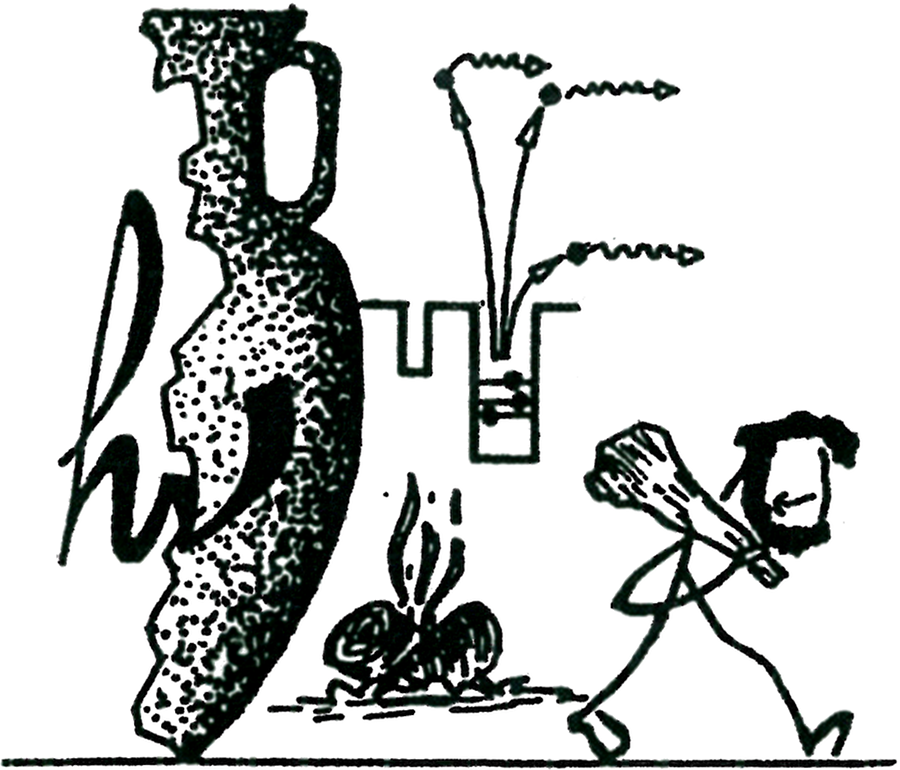
\includegraphics[width=5cm]{logo_CRPAA}
        \end{minipage}%
        \hfill%
        \begin{minipage}{12cm}
          \RaggedLeft
          Université de Bordeaux~3 -- Université de Bordeaux~1

          3\ieme~cycle -- \textbf{D.E.S.S.}\\
          \textbf{\frquote{MÉTHODES PHYSIQUES EN ARCHÉOLOGIE ET 
          MUSÉOGRAPHIE}}

          COMPTE RENDU DU STAGE DE RECHERCHE EFFECTUÉ AU\\
          \textbf{C.R.P.A.A.} \quad UMR CNRS~5060\\
          \textbf{C}entre de \textbf{R}echerche en \textbf{P}hysique 
          \textbf{A}ppliquée à L'\textbf{A}rchéologie\\
          \textbf{Maison de l'archéologie,} Esplanade des Antilles, 
          Domaine Universitaire,\\
          33607 - PESSAC cedex, FRANCE\\
          Tél. : 05.57.12.45.53 \quad Fax : 05.57.12.45.50
        \end{minipage}
      } ;
    \end{tikzpicture}
  } ;
\end{tikzpicture}

\begin{tikzpicture}[
  remember picture, overlay, anchor=south,
  inner sep=0, outer sep=1cm,
]
  \node at (current page.south) {
    \begin{tikzpicture}
      \node (F) at (0.00, 0.00) [%
        % below=1cm of E.south, 
        draw, thick, 
        text width=0.85\paperwidth, 
        inner sep=3pt,
      ] {%
        \small Juin~2000 \hfill 
        MÉMOIRES DE LA SÉRIE \textbf{\frquote{FORMATION À ET PAR LA 
        RECHERCHE}} \hfill 
        \textbf{\no441.} DESS
      } ;
    \end{tikzpicture}
  } ;
\end{tikzpicture}

\begin{center}
\vfill

{\LARGE
Programme PACT ARCHI-MED Glaçures -- II\par
}

\rule{.5\textwidth}{1pt}

{\bfseries\huge
\MakeUppercase{Contribution à la réhabilitation architecturale du 
\PaM, Meknès, Maroc, \siecle{xvii}}

\bigskip

Recherche des caractéristiques physiques de zelliges de pavement
}

\vfill

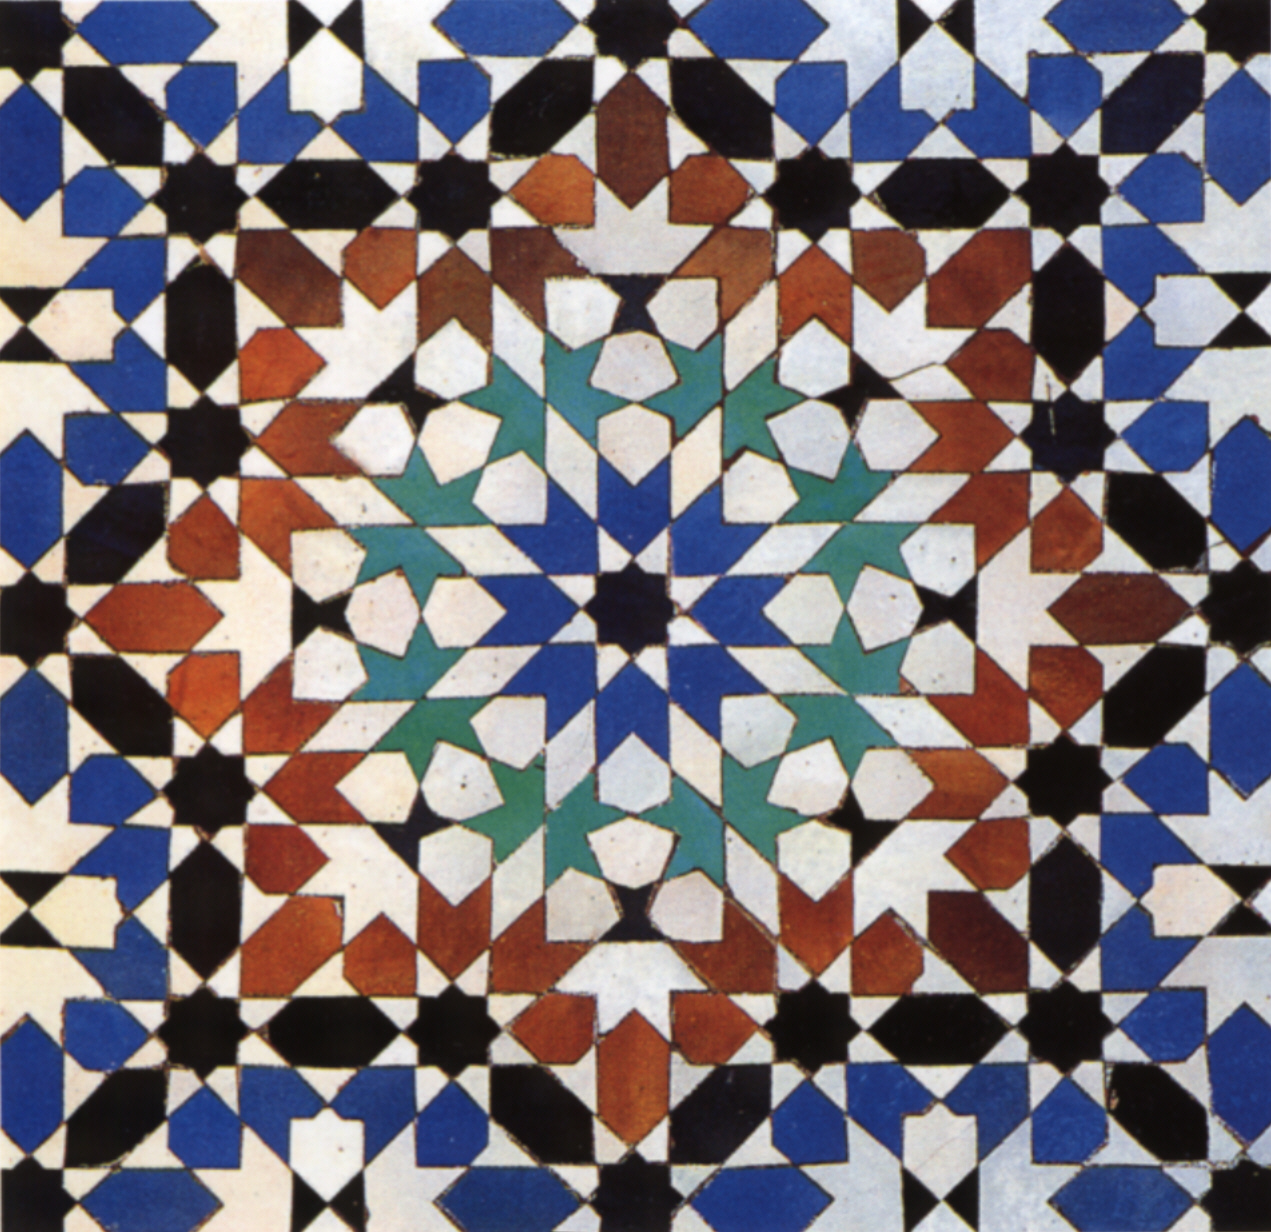
\includegraphics[width=10cm]{zellige_01}

\vfill

\textbf{\Large LABETOULLE Sonia}

\emph{Maître ès Sciences\\(Chimie physique)}\par
\end{center}
}

\makeatother





% \newcommand{\sclnum}[1]{\bsc{#1}\ieme}
% \newcommand{\scl}[1]{\sclnum{#1}~s.}
% \renewcommand{\siecle}[1]{\sclnum{#1}~siècle}


%!TEX root = MemoireZelliges.tex

% Numéros de siècles
% ==================
\newcommand{\sieclenum}[1]{%
  \ifrmnum{#1}{%
    \bsc{\MakeLowercase{#1}}%
    \ifstrequal{#1}{i}{\ier}{\ieme}%
  }{%
    \bsc{\MakeLowercase{\romannumeral#1}}%
    \ifnumequal{#1}{1}{\ier}{\ieme}%
  }%
}
\newcommand{\siecle}[2][siècle]{%
  \sieclenum{#2}~#1%
}
\newcommand{\sieclelist}[2]{%
  \sieclenum{#1} et \sieclenum{#2}~siècles%
}
\newcommand{\sieclerange}[2]{%
  \sieclenum{#1}-\sieclenum{#2}~siècles%
}

% Incise
% ======
\DeclareRobustCommand{\oinc}{\textemdash~}
\DeclareRobustCommand{\finc}{~\textemdash}
\DeclareRobustCommand{\incise}[1]{\oinc#1\finc}
\DeclareRobustCommand{\oincise}[1]{\oinc#1}

% Coloration en cas de brouillon
% ==============================
\providecommand{\colordraft}[2]{%
  \texorpdfstring{%
    \ifbool{draft}
           {\hspace*{0pt}{\color{#1}#2}}
           {#2}%
  }{%
    #2%
  }%
}

\newcommand{\gens}[2][]{%
  \colordraft{orange}{\notblank{#1}{#1~}{}\bsc{#2}}%
}
\newcommand{\SL}{\gens[Sonia]{Labetoulle}\xspace}
\newcommand{\FB}{\gens[Françoise]{Bechtel}\xspace}
\newcommand{\MS}{\gens[Max]{Schv\oe{}rer}\xspace}
\newcommand{\ABA}{\gens[Ayed]{Ben Amara}\xspace}
\newcommand{\CRPAA}{%
  \emph{%
    Centre de Recherche en Physique Appliquée à l'Archéologie%
  }\xspace%
}


\DeclareRobustCommand{\arabzell}{%
  \texorpdfstring{\RL{zly^g}}{}%
}

\newcommand{\blackstar}{\ding{88}}
\newcommand{\bluestar}{{\color{blue}\ding{88}}}

\newcommand{\bdx}[1]{%
  \texorpdfstring{BDX\,#1\xspace}{BDX#1}%
}

\newcommand{\PaM}{\colordraft{red}{Palais al-Mansour}\xspace}
% \newcommand{\PaM}{palais Al-Mansour\xspace}

\newcommand{\Zell}[2][]{%
  Zellige#1 monochrome#1 #2 provenant du \PaM, \siecle{17}\xspace
}

\newcommand{\legendeA}{Meknès (Maroc), \bdx{6528}. \Zell{vert}}
\newcommand{\legendeB}{Meknès (Maroc), \bdx{6529}. \Zell{bleu vert}}
\newcommand{\legendeC}{Meknès (Maroc), \bdx{6530}. \Zell{noir}}
\newcommand{\legendeD}{Meknès (Maroc), \bdx{6531}. \Zell{miel}}
\newcommand{\legendeE}{Meknès (Maroc), \bdx{6532}. \Zell{blanc}}

\newcommand{\legendeAll}{%
  Meknès (Maroc), \bdx{6528}, \bdx{6529}, \bdx{6530}, \bdx{6531} et 
  \bdx{6532}. \Zell[s]{vert, bleu, noir, miel et blanc}%
}

\newcommand{\zlaygi}{\emph{\colordraft{red}{zl\={a}y\v{g}\={\i}}}\xspace}
\newcommand{\hatim}{\emph{\colordraft{red}{h\={a}tim}}\xspace}
\newcommand{\saft}{\emph{\colordraft{red}{\d{s}aft}}\xspace}
\newcommand{\manqas}{\emph{\colordraft{red}{manq\={a}\v{s}}}\xspace}
\newcommand{\naqs}{\emph{\colordraft{red}{naq\v{s}}}\xspace}
\newcommand{\fars}{\emph{\colordraft{red}{far\v{s}}}\xspace}
\newcommand{\tafrisa}{\emph{\colordraft{red}{tafr\={\i}\v{s}a}}\xspace}
\newcommand{\zillig}{\emph{\colordraft{red}{zill\={\i}\v{g}}}\xspace}
\newcommand{\furma}{\emph{\colordraft{red}{f\={u}rma}}\xspace}
\newcommand{\furmas}{\emph{\colordraft{red}{f\={u}rmas}}\xspace}
\newcommand{\farina}{\emph{\colordraft{red}{far\={\i}na}}\xspace}
\newcommand{\mzihrinayy}{\emph{\colordraft{red}{mzihr\={\i} nayy}}\xspace}
\newcommand{\alqala}{\emph{\colordraft{red}{al-q\={a}la}}\xspace}
\newcommand{\tansif}{\emph{\colordraft{red}{tans\={\i}f}}\xspace}
\newcommand{\tagfif}{\emph{\colordraft{red}{ta\v{g}f\={\i}f}}\xspace}
\newcommand{\zwabi}{\emph{\colordraft{red}{zw\={a}b\={\i}}}\xspace}
\newcommand{\maallem}{\emph{\colordraft{red}{maallem}}\xspace}

\newcommand{\Pe}{\ensuremath{P_\text{e}}}
\newcommand{\Xn}{\ensuremath{X_\text{n}}}
\newcommand{\Yn}{\ensuremath{Y_\text{n}}}
\newcommand{\Zn}{\ensuremath{Z_\text{n}}}
\newcommand{\CIEL}{\ensuremath{L^\text{*}}\xspace}
\newcommand{\CIEa}{\ensuremath{a^\text{*}}\xspace}
\newcommand{\CIEb}{\ensuremath{b^\text{*}}\xspace}
\newcommand{\CIELb}{\ensuremath{\bm{L^\text{*}}}\xspace}
\newcommand{\CIEab}{\ensuremath{\bm{a^\text{*}}}\xspace}
\newcommand{\CIEbb}{\ensuremath{\bm{b^\text{*}}}\xspace}
\newcommand{\CIEY}{\ensuremath{Y}\xspace}
\newcommand{\CIEx}{\ensuremath{x}\xspace}
\newcommand{\CIEy}{\ensuremath{y}\xspace}
\newcommand{\CIEz}{\ensuremath{z}\xspace}
\newcommand{\CIEYb}{\ensuremath{\bm{Y}}\xspace}
\newcommand{\CIExb}{\ensuremath{\bm{x}}\xspace}
\newcommand{\CIEyb}{\ensuremath{\bm{y}}\xspace}
\newcommand{\CIEzb}{\ensuremath{\bm{z}}\xspace}
\newcommand{\Yxy}{\ensuremath{\CIEY\!\!\CIEx\CIEy}\xspace}
\newcommand{\Lab}{\ensuremath{\CIEL\!\!\CIEa\!\CIEb}\xspace}
\newcommand{\WLd}{\ensuremath{\lambda_\text{d}}\xspace}
\newcommand{\WLdb}{\ensuremath{\bm{\lambda_\text{d}}}\xspace}

\definecolor{RED}{named}{red}

\newcommand{\spectro}{\colordraft{red}{spectrométrie}\xspace}
\newcommand{\carto}{\colordraft{red}{cartographie}\xspace}
\newcommand{\trichro}{\colordraft{red}{trichromatique}\xspace}
\newcommand{\trichros}{\colordraft{red}{trichromatiques}\xspace}
\newcommand{\cristallo}{\colordraft{red}{cristallographique}\xspace}
\newcommand{\cristallos}{\colordraft{red}{cristallographiques}\xspace}

\newcommand{\RX}{\colordraft{red}{rayons~X}\xspace}
\newcommand{\DX}[1][d]{\colordraft{red}{#1iffraction de \RX{}}\xspace}
\newcommand{\MEB}[1][e]{\colordraft{red}{microscop#1 électronique à balayage}\xspace}
\newcommand{\CL}{\colordraft{red}{cathodoluminescence}\xspace}
\newcommand{\AO}{\colordraft{red}{absorption optique}\xspace}
\newcommand{\SAO}{\colordraft{red}{\spectro d'\AO{}}\xspace}
\newcommand{\ERD}{\colordraft{red}{électrons rétrodiffusés}\xspace}
\newcommand{\EDS}{\colordraft{red}{\spectro de \RX en dispersion d'énergie}\xspace}
\newcommand{\CHRO}{\colordraft{red}{chromamétrie}\xspace}

\newcommand{\DimText}{%
  \emph{Dimensions} (L\,\texttimes\,l\,\texttimes\,e)\xspace%
}

\newcommand{\PMO}{\colordraft{red}{\si{\percent} massique d'oxyde}\xspace}
\newcommand{\zone}[2]{\colordraft{red}{zone analysée : \SI{#1}{#2}}\xspace}


\newcommand{\albite}{\colordraft{red}{\ch{NaAlSi3O8}}\xspace}
\newcommand{\gehlenite}{\colordraft{red}{\ch{Ca2Al2SiO7}}\xspace}
\newcommand{\anorthite}{\colordraft{red}{\ch{CaAl2Si2O8}}\xspace}
\newcommand{\diopside}{\colordraft{red}{\ch{CaMg(SiO3)2}}\xspace}
\newcommand{\diopsideal}
           {\colordraft{red}{\ch{Ca(Mg{,}Al)(Si{,}Al)2O6)}}\xspace}
\newcommand{\diopsidealfe}
           {\colordraft{red}{\ch{Ca(Mg{,}Fe{,}Al)(Si{,}Al)2O6)}}\xspace}
\newcommand{\calcite}{\colordraft{red}{\ch{CaCO3}}\xspace}
\newcommand{\quartz}{\colordraft{red}{\ch{SiO2}}\xspace}
\newcommand{\cassiterite}{\colordraft{red}{\ch{SnO2}}\xspace}

% \ce{(I+)^*}
% \ce{(I+)^*}
% \ce{(I+)^*}
% \ce{(I+)}
% \ce{(I+)}
% \ce{(I+)}
% \ce{Al2O3}
% \ce{Al2O3}
% \ce{Ca(Mg{,}Al)(Si{,}Al)2O6}
% \ce{Ca(Mg{,}Al)(Si{,}Al)2O6}
% \ce{Ca(Mg{,}Fe{,}Al)(Si{,}Al)2O6)}   diopside alumineux
% \ce{Ca2Al2SiO7}                      gehlénite
% \ce{Ca2Al2SiO7}                      gehlénite
% \ce{Ca2Al2SiO7}                      gehlénite
% \ce{Ca2Al2SiO7}                      gehlénite
% \ce{CaAl2Si2O8}                      anorthite
% \ce{CaAl2Si2O8}                      anorthite
% \ce{CaAl2Si2O8}                      anorthite
% \ce{CaCO3}
% \ce{CaCO3}
% \ce{CaCO3}
% \ce{CaCO3}
% \ce{CaCO3}
% \ce{CaCO3}
% \ce{CaCO3}
% \ce{CaMg(SiO3)2}                     diopside
% \ce{CaO}
% \ce{CaO}
% \ce{CaO}
% \ce{Co^2+}
% \ce{Co^2+}
% \ce{Co^2+}
% \ce{Co^2+}
% \ce{Co^2+}
% \ce{Cu^2+}
% \ce{Cu^2+}
% \ce{Cu^2+}
% \ce{Cu^2+}
% \ce{Cu^2+}
% \ce{Cu^2+}
% \ce{CuO}
% \ce{CuO}
% \ce{Fe2O3}                        hématite
% \ce{Fe2O3}
% \ce{Fe2O3}
% \ce{Fe2O3}
% \ce{Fe2O3}
% \ce{Fe2O3}
% \ce{Fe2O3}
% \ce{Fe2O3}
% \ce{Fe^3+}
% \ce{Fe^3+}
% \ce{Fe^3+}
% \ce{Fe^3+}
% \ce{Fe^3+}
% \ce{Fe^3+}
% \ce{Fe^3+}
% \ce{Fe^3+}
% \ce{Fe^3+}
% \ce{Fe^3+}
% \ce{Fe^3+}
% \ce{Fe^3+}
% \ce{Fe^3+}
% \ce{Fe^3+}
% \ce{Fe^3+}
% \ce{Fe^3+}
% \ce{Fe^3+}
% \ce{Fe^3+}
% \ce{Fe^3+}
% \ce{Fe^3+}
% \ce{Fe^3+}
% \ce{Fe^3+}
% \ce{Fe^3+}
% \ce{Fe^3+}
% \ce{Fe^3+}
% \ce{Fe^3+}
% \ce{Fe^3+}
% \ce{He}
% \ce{K2O}
% \ce{K2O}
% \ce{MgO}
% \ce{MgO}
% \ce{Mn^3+}
% \ce{Mn^3+}
% \ce{Mn^3+}
% \ce{Mn^3+}
% \ce{Mn^3+}
% \ce{MnO}
% \ce{MnO}
% \ce{Na2O}
% \ce{Na2O}
% \ce{NaAlSi3O8}                              albite
% \ce{NaAlSi3O8}                              albite
% \ce{NaAlSi3O8}                              albite
% \ce{PbO}
% \ce{PbO}
% \ce{PbO}
% \ce{Si(Li)}
% \ce{SiO2}
% \ce{SiO2}
% \ce{SiO2}
% \ce{SiO2}
% \ce{SiO2}
% \ce{SiO2}
% \ce{SiO2}
% \ce{SiO2}
% \ce{SiO2}
% \ce{SiO2}
% \ce{SiO2}
% \ce{SiO2}
% \ce{SiO2}
% \ce{SiO2}
% \ce{SnO2}
% \ce{SnO2}
% \ce{SnO2}
% \ce{SnO2}
% \ce{TiO2}

%!TEX root = MemoireZelliges.tex

% .. tabular for chemical composition ..
% ======================================
\newenvironment{cartotab}
  {%
    \smaller%
    \noindent\ignorespaces
    \tabular{R{0.9cm} @{\ =\ } S @{\ $\pm$\ } S @{\hspace*{3em}}
             R{0.9cm} @{\ =\ } S @{\ $\pm$\ } S @{\hspace*{3em}} 
             R{0.9cm} @{\ =\ } S @{\ $\pm$\ } S @{\hspace*{3em}} 
             R{0.9cm} @{\ =\ } S @{\ $\pm$\ } S }%
      \toprule
  }
  {%
      \midrule
        \cartolgntt
      \bottomrule
    \endtabular%
  }
\newcommand{\cartolgn}[3]{\ce{#1}  & #2  & #3}
\newcommand{\cartolgnnd}[1]{\ce{#1}  & \multicolumn{2}{c}{\emph{nd}}}
\newcommand{\cartolgntt}{%
  \multicolumn{10}{r}{\RaggedLeft Total :} & 
  \multicolumn{2}{S}{100.00}
  \tabularnewline
}


% .. tabular for chromametry result ..
% ====================================
\newcommand{\chrolgna}[9]{%
  #1 & #2 & #3 & #4 & #5 & #6 & #7 & #8 & #9
}
\newcommand{\chrolgnb}[5]{%
  \mbox{#1} {\normalfont(\mbox{#2} \mbox{\SIrange{#3}{#4}{\nm}#5})}
}
\NewEnviron{chrotab}[1][Zone\\étudiée]{%
  \renewcommand{\tabularxcolumn}[1]{M{##1}}
  % \sisetup{%
  %   table-figures-integer=4,
  %   table-figures-decimal=3
  % }
  \noindent\ignorespaces%
  \smaller%
  \setlength{\tabcolsep}{0pt}%
  \begin{tabularx}{1.0\textwidth}
                  {>{\bfseries}M{2cm}                @{\qquad}
                   S@{\hspace{1ex}}S                 @{\qquad} 
                   S@{\hspace{1ex}}S@{\hspace{1ex}}S @{\qquad} 
                   S@{\hspace{1ex}}S@{\hspace{1ex}}S @{\qquad} 
                   >{\bfseries}X}
      \multirow{2}{2cm}{#1}     & 
      {$\lambda_D$} & {$P_e$}   &
      \multirow{2}{2em}{{$Y$}}  & 
      \multirow{2}{2em}{{$x$}}  & 
      \multirow{2}{2em}{{$y$}}  & 
      \multirow{2}{2em}{{$L*$}} & 
      \multirow{2}{2em}{{$a*$}} & 
      \multirow{2}{2em}{{$b*$}} & 
      \multirow{2}{2cm}{Couleur associée}
    \tabularnewline
       & 
      {(\si{\nm})} & {(\si{\percent})} &
       & & & & & &
    \tabularnewline
    \otoprule

    \BODY

    \bottomrule
  \end{tabularx}%
}

%!TEX root = MemoireZelliges.tex

\newcommand{\drawhatim}{%
  (    0.000 , {sqrt(2)}) -- ({1-sqrt(2)},     1.000 ) --
  (   -1.000 ,    1.000 ) -- (    -1.000 ,{sqrt(2)-1}) --
  ({-sqrt(2)},    0.000 ) -- (    -1.000 ,{1-sqrt(2)}) --
  (   -1.000 ,   -1.000 ) -- ({1-sqrt(2)},    -1.000 ) --
  (    0.000 ,-{sqrt(2)}) -- ({sqrt(2)-1},    -1.000 ) --
  (    1.000 ,   -1.000 ) -- (     1.000 ,{1-sqrt(2)}) --
  ( {sqrt(2)},    0.000 ) -- (     1.000 ,{sqrt(2)-1}) --
  (    1.000 ,    1.000 ) -- ({sqrt(2)-1},     1.000 ) -- cycle
}

\newcommand{\drawluza}{%
  (     0.000 ,   0.000 ) -- ({2-sqrt(2)},     0.000 ) -- 
  ({2-sqrt(2)},{sqrt(2)}) -- ({1-sqrt(2)},{sqrt(2)-1}) -- cycle
}

\newcommand{\drawsaft}{%
  (-2.00, 0.00) -- (-1.00, 1.00) -- ( 1.00, 1.00) -- 
  ( 2.00, 0.00) -- ( 1.00,-1.00) -- (-1.00,-1.00) -- cycle
}

% % Fawrkat
% \fill [color=ffqqff, fill=ffqqff, fill opacity=0.1] 
%       ( 0.414,-1.000) -- (-1.000,-1.000) -- 
%       (-2.000, 0.000) -- (-1.000, 1.000) -- 
%       ( 0.414, 1.000) -- ( 0.414, 0.414) -- 
%       ( 0.000, 0.000) -- ( 0.414,-0.414) -- cycle ;

\newcommand{\squeletteb}{%
  \draw [domain=-1:1] plot( \x, {-\x} ) ;
  \draw [domain=-2:2] plot( 0, \x ) ;
  \draw [domain=0:{2-2*sqrt(2)}] plot(-2, \x ) ;
  \draw [domain=0:{2*sqrt(2)-2}] plot( 2, \x ) ;
  \draw [domain=-2:2] plot( \x, {+sqrt(2)} ) ;
  \draw [domain=-2:2] plot( \x, {-sqrt(2)}   ) ;
  \draw [domain=0:5]  plot( \x, {+sqrt(2)+2} ) ;
  \draw [domain=-5:0] plot( \x, {-sqrt(2)-2}   ) ;

  \draw [domain=2:1] plot(\x, {-\x + 2*sqrt(2)}) ;
  \draw [domain=-2:-1] plot(\x, {-\x - 2*sqrt(2)}) ;

  \draw [domain=-1:-3] plot( \x, {\x + 2}) ;
  \draw [domain=1:3] plot( \x, {\x - 2}) ;
  \draw [domain=-6:-2] plot( \x, {\x + 2*sqrt(2) + 2}) ;
  \draw [domain=2:6] plot( \x, {\x - 2*sqrt(2) - 2}) ;

  \filldraw [shift={( 1 , {-sqrt(2)-1} )}] 
    \drawhatim ;
  \filldraw [shift={( -1 , {sqrt(2)+1} )}] 
    \drawhatim ;
  \filldraw [shift={( {-2*sqrt(2)-3} , {-sqrt(2)-1} )}] 
    \drawhatim ;
  \filldraw [shift={( {2*sqrt(2)+3} , {sqrt(2)+1} )}] 
    \drawhatim ;

  \filldraw [shift={( {-sqrt(2)-1} , {-sqrt(2)-1} )}] 
    \drawsaft ;
  \filldraw [shift={( {sqrt(2)+1} , {sqrt(2)+1} )}] 
    \drawsaft ;
  \filldraw [shift={( {-sqrt(2)-2} , 0 )}, rotate=45] 
    \drawsaft ;
  \filldraw [shift={( {sqrt(2)+2} , 0 )}, rotate=45] 
    \drawsaft ;
}

\newcommand{\squelettea}{%
  \begin{scope}
    \clip (-4,-4) rectangle (4,4) ;
    \draw plot( \x, {\x + sqrt(2)}) ;
    \draw plot( \x, {\x - sqrt(2)}) ;
    \draw plot(-\x, {\x + sqrt(2)}) ;
    \draw plot(-\x, {\x - sqrt(2)}) ;
  \end{scope}

  \draw ( {-1-sqrt(2)} , {-1-sqrt(2)} ) rectangle
        ( {+1+sqrt(2)} , {+1+sqrt(2)} ) ;
  \draw ( {-3-sqrt(2)} , {-3-sqrt(2)} ) rectangle
        ( {+3+sqrt(2)} , {+3+sqrt(2)} ) ;

  \filldraw [shift={( {+2+sqrt(2)} , {+2+sqrt(2)} )}] 
    \drawhatim ;
  \filldraw [shift={( {+2+sqrt(2)} , {-2-sqrt(2)} )}] 
    \drawhatim ;
  \filldraw [shift={( {-2-sqrt(2)} , {+2+sqrt(2)} )}] 
    \drawhatim ;
  \filldraw [shift={( {-2-sqrt(2)} , {-2-sqrt(2)} )}] 
    \drawhatim ;

  \filldraw [shift={( 0 , {-2-sqrt(2)} )}] 
    \drawsaft ;
  \filldraw [shift={( 0 , {+2+sqrt(2)} )}] 
    \drawsaft ;
  \filldraw [shift={( {-2-sqrt(2)} , 0 )} , rotate=90] 
    \drawsaft ;
  \filldraw [shift={( {+2+sqrt(2)} , 0 )} , rotate=90] 
    \drawsaft ;
}

\newcommand{\drawfluoX}{%
  ( 0.19,-0.32) .. controls ( 0.22,-0.40) and ( 0.23,-0.43) ..
  ( 0.50,-0.79) .. controls ( 0.60,-0.95) and ( 0.66,-1.12) ..
  ( 0.66,-1.32) .. controls ( 0.65,-1.78) and ( 0.30,-1.98) ..
  ( 0.00,-1.98) .. controls (-0.30,-1.98) and (-0.65,-1.78) ..
  (-0.66,-1.32) .. controls (-0.65,-1.12) and (-0.60,-0.95) ..
  (-0.50,-0.79) .. controls (-0.23,-0.43) and (-0.22,-0.40) ..
  (-0.19,-0.32)
}

\newcommand{\drawRX}{%
  ( 0.15,-0.06) to [out=-87, in=104] 
  ( 0.19,-0.32) .. controls ( 0.21,-0.40) and ( 0.23,-0.46) ..
  ( 0.26,-0.51) .. controls ( 0.31,-0.60) and ( 0.35,-0.65) ..
  ( 0.41,-0.74) .. controls ( 0.57,-0.99) and ( 0.66,-1.30) ..
  ( 0.50,-1.54) .. controls ( 0.39,-1.71) and ( 0.24,-1.81) ..
  ( 0.00,-1.81) .. controls (-0.24,-1.81) and (-0.39,-1.71) ..
  (-0.50,-1.54) .. controls (-0.66,-1.30) and (-0.57,-0.99) ..
  (-0.41,-0.74) .. controls (-0.35,-0.65) and (-0.31,-0.60) ..
  (-0.26,-0.51) .. controls (-0.23,-0.46) and (-0.21,-0.40) ..
  (-0.19,-0.32) to [out=76, in=-93] 
  (-0.15,-0.06)
}

\newcommand{\drawinterne}{%
  ( 0.11,-0.06) .. controls ( 0.13,-0.46) and ( 0.23,-0.53) .. 
  ( 0.34,-0.71) .. controls ( 0.50,-0.96) and ( 0.56,-1.21) .. 
  ( 0.42,-1.43) .. controls ( 0.32,-1.59) and ( 0.19,-1.65) .. 
  ( 0.00,-1.65) .. controls (-0.19,-1.65) and (-0.32,-1.59) .. 
  (-0.42,-1.43) .. controls (-0.56,-1.21) and (-0.50,-0.96) .. 
  (-0.34,-0.71) .. controls (-0.23,-0.53) and (-0.13,-0.46) .. 
  (-0.11,-0.06)
}

\newcommand{\drawaugier}{%
  (-0.15, 0.00) rectangle ( 0.15, -0.06)
}

\newcommand{\MEBpoire}{%
  \begin{scope}[
    scale=2.3,
    every node/.style={font=\scriptsize},
    line cap=round,
  ]

    \pgfmathsetmacro{\xA}{0.145}
    \pgfmathsetmacro{\yA}{-0.35}
    \pgfmathsetmacro{\xB}{0.495}
    \pgfmathsetmacro{\yB}{-1.11}
    \coordinate (A1) at (-\xA, \yA) ;
    \coordinate (A2) at ( \xA, \yA) ;
    \coordinate (B1) at (-\xB, \yB) ;
    \coordinate (B2) at ( \xB, \yB) ;

    % .. Remplissage ..
    % ... Fluo X ...
    \fill [DarkSlateBlue!20!white] \drawfluoX ;
    % ... RX ...
    \fill [DarkSlateBlue!30!white] \drawRX ;
    % ... RX carac ...
    \fill [DarkSlateBlue!40!white] \drawinterne ;

    \begin{scope}
      \clip \drawinterne ;
      % ... Secondaires ...
      \fill [DarkSlateBlue!50!white] 
            (-\xB, \yB) rectangle ( \xB, \yA) ;
      % ... Rétrodiff ...
      \fill [DarkSlateBlue!60!white] 
            (-\xA, \yA) rectangle ( \xA, 0.00) ;
    \end{scope}
    % Électrons Augier
    \fill [fill=DarkSlateBlue!70!white] \drawaugier ;

    % .. Contours ..
    \begin{scope}[DarkSlateBlue]
      % ... Fluo X ...
      \draw \drawfluoX ;
      % ... RX ...
      \draw \drawRX ;
      % ... RX carac ...
      \draw \drawinterne ;
      % Limite secondaires / rétrodiff
      \draw (A1) -- (A2) ;
      % limite rétrodiff / RC carac
      \draw (B1) -- (B2) ;
      % Électrons Augier
      \draw \drawaugier ;
    \end{scope}

    % .. Faisceau incident ..
    \filldraw [draw=DarkRed, bottom color=DarkRed, top color=white]
          (-0.30, 0.77) -- (-0.15, 0.00) -- ( 0.00,  0.00) -- 
          ( 0.15, 0.00) -- ( 0.30, 0.77) 
          node (G) {} ;

    % .. Surface échantillon ..
    \draw [thick]
          (-1.40, 0.00) -- ( 1.40, 0.00) 
          node (H) [pos=1] {} ;

    % .. Légende ..
    \coordinate (A1) at (-0.10,-0.03) ;
    \coordinate (A2) at (-0.50,-0.15) ;
    \coordinate (B1) at (-0.05,-0.20) ;
    \coordinate (B2) at (-0.50,-0.45) ;
    \coordinate (C1) at ( 0.10,-0.80) ;
    \coordinate (C2) at ( 0.80,-0.80) ;
    \coordinate (D1) at ( 0.20,-1.30) ;
    \coordinate (D2) at ( 0.80,-1.30) ;
    \coordinate (E1) at (-0.50,-1.40) ;
    \coordinate (E2) at (-0.80,-1.40) ;
    \coordinate (F1) at (-0.50,-1.65) ;
    \coordinate (F2) at (-0.80,-1.75) ;
  \end{scope}
}

\newcommand{\MEBlegende}{%
  % .. Légende ..
  \begin{scope}[every node/.style={font=\smaller}]
    \draw (A1) -- (A2) 
          node [left] {électrons Auger} ;
    \draw (B1) -- (B2) 
          node [left, align=right] {électrons\\secondaires} ;
    \draw (C1) -- (C2) 
          node [right, align=left] {électrons\\rétrodiffusés} ;
    \draw (D1) -- (D2) 
          node [right, align=left] {\RX\\caractéristiques} ;
    \draw (E1) -- (E2) 
          node [left, align=right] {continuum\\de \RX} ;
    \draw (F1) -- (F2) 
          node [left] {fluorescence~X} ;
    \node [below right, align=left] at (G) 
          {faisceau incident\\d'électrons} ;
    \node [right, align=left] at (H) {surface de\\l'échantillon} ;
  \end{scope}
}

\newcommand{\CLapp}{%
  \begin{scope}[
    scale=0.1, 
    rounded corners=0.5, 
    >=stealth', 
    thick,
  ]
    % \draw [help lines, step=1, ultra thin, densely dotted] 
    %       (-40.00,-10.00) grid ( 40.00, 60.00) ;
    % \draw [help lines, step=5, ultra thin] 
    %       (-40.00,-10.00) grid ( 40.00, 60.00) ;

    \begin{scope}
      % Moniteur
      \draw ( 0.00,  0.00) rectangle ++ ( 30.00, 24.00) ;
      \draw ( 2.00,  8.00) rectangle ++ ( 26.00, 14.00) ;
      \draw ( 2.00,  2.00) rectangle ++ (  2.00,  2.00) ;
      % Système d'acquisition
      \draw ( 0.00, 28.00) rectangle ++ ( 30.00,  6.00) ;
      \draw ( 0.00, 38.00) rectangle ++ ( 30.00,  6.00) ;
      \draw ( 0.00, 48.00) rectangle ++ ( 30.00,  6.00) ;
    \end{scope}

    \begin{scope}[shift={(-15.00, 20.00)}]
      % Loupe bino
      \draw ( 2.00,  0.00) -- ( 5.80,  4.80) -- ( 5.80, 16.20) --
            ( 2.90, 16.20) -- ( 2.90, 21.20) -- ( 3.10, 21.30) -- 
            ( 3.10, 22.90) -- ( 3.70, 23.40) -- ( 3.70, 24.10) -- 
            (-3.70, 24.10) -- (-3.70, 23.40) -- (-3.10, 22.90) -- 
            (-3.10, 21.30) -- (-2.90, 21.20) -- (-2.90, 16.20) -- 
            (-5.80, 16.20) -- (-5.80,  4.80) -- (-2.00,  0.00) -- 
            cycle
         ;
      \draw (-2.00, 0.00) -- (-1.00, 1.00) -- 
            ( 1.00, 1.00) -- ( 2.00, 0.00) ;
      \draw (-2.90, 21.20) -- ( 2.90, 21.20) ;
      \draw (-3.10, 22.90) -- ( 3.10, 22.90) ;
      \draw (-2.90, 18.70) arc (113.4:66.6:7.3) ;
      \draw (-2.90, 18.70) arc (-113.4:-66.6:7.3) ;

      % Caméra CCD
      \draw [shift={( 0.00, 30.00)}, pattern=north west lines]
            ( 4.00,-5.90) -- ( 4.00,-3.50) -- ( 6.00,-3.50) -- 
            ( 6.00, 3.50) -- (-1.60, 3.50) -- (-1.60, 4.80) -- 
            (-3.60, 4.80) -- (-3.60, 3.50) -- (-5.70, 3.50) -- 
            (-7.00, 0.70) -- (-7.00,-0.70) -- (-5.70,-3.50) -- 
            (-4.00,-3.50) -- (-4.00,-5.90) -- cycle
         ;
    \end{scope}

    % Chambre Nuclide
    \begin{scope}[shift={(-27.00, 7.00)}]
      \draw ( 0.00, 0.00) rectangle ++ ( 20.00, 8.00) ;
      \filldraw ( 0.00, 5.00) arc (90:-90:1) ;

      \begin{scope}[shift={( 9.00, 3.25)}]
        \draw ( 0.00, 0.00) rectangle ++ ( 3.00, 1.50) ;
        \draw [->, decorate, decoration={snake, 
               amplitude=.5mm, segment length=2mm, post length=2mm}]
              ( 1.50, 1.5) -- ++ ( 1.50, 8.25) ;
      \end{scope}

      \draw [->] 
            ( 2.00, 4.00) -- ( 7.00, 4.00) 
            node [midway, above] {$e^-$} ;
    \end{scope}

    % Liens
    \draw ( 15.00, 24.00) -- ++ ( 0.00, 4.00) ;
    \draw ( 15.00, 34.00) -- ++ ( 0.00, 4.00) ;
    \draw ( 15.00, 44.00) -- ++ ( 0.00, 4.00) ;
    \draw ( 15.00, 54.00) -- ++ ( 0.00, 4.00) -- ++ 
          (-30.00,  0.00) -- ++ ( 0.00,-4.50) ;

    % % Légende
    \coordinate (A) at (-28.00, 11.00) ;
    \coordinate (B) at (-22.00, 30.00) ;
    \coordinate (C) at (-23.00, 50.00) ;
    \coordinate (D) at ( 31.00, 11.00) ;
    \coordinate (E) at ( 32.00, 54.00) ;
    \coordinate (F) at ( 32.00, 28.00) ;
  \end{scope}
}

\newcommand{\CLappL}{%
  % Légende
  \begin{scope}[every node/.style={font=\smaller}]
    \node [left, align=right] at (A) {chambre\\Nuclide} ;
    \node [left, align=right] at (B) {loupe\\binoculaire} ;
    \node [left, align=right] at (C) {caméra\\3CCD} ;
    \node [right, align=left] at (D) {moniteur} ;

    \draw [decorate, decoration=brace] (E) -- (F)
          node [midway, right, align=left] 
               {système d'acquisition\\et de traitement} ;
  \end{scope}
}

\newcommand{\CLpcp}{%
  \begin{scope}[>=stealth', every node/.style={font=\smaller}]

    % \draw [help lines, densely dotted, red, step=1] 
    %       (-10.00, -20.00) grid ( 60.00, 50.00) ;
    % \draw [help lines, ultra thin, red, step=5] 
    %       (-10.00, -20.00) grid ( 60.00, 50.00) ;

    \begin{scope}[every node/.style={font=\smaller}, darkgray]
      \draw [->] 
            (-0.20,-1.00) -- (-0.20, 5.50) 
            node [below right, align=left] {énergie\\relative} ;
      \node at (-0.80, 4.20) {BC} ;
      \node at (-0.80, 1.75) {BI} ;
      \node at (-0.80,-0.70) {BV} ;
    \end{scope}

    \begin{scope}[thick, pattern=north east lines]
      \filldraw ( 0.50,-0.50) circle (0.20) ;
      \filldraw ( 4.20,-0.50) circle (0.20) ;
    \end{scope}

    \begin{scope}[thick]
      \draw (-0.70, 0.00) -- ( 5.00, 0.00) ;
      \draw (-0.70, 3.50) -- ( 1.20, 3.50) -- 
            ( 1.20, 1.75) -- ( 2.00, 1.75) -- 
            ( 2.00, 3.50) -- ( 5.00, 3.50) ; 
      \draw ( 3.20, 2.50) -- ( 4.20, 2.50) 
            node [right] {\ch{(I+)^*}} ;
      \draw ( 2.50, 1.00) -- ( 4.20, 1.00) 
            node [right] {\ch{(I+)}} ;
    \end{scope}

    \begin{scope}[->, densely dotted, thick, DarkSlateBlue]
      \draw ( 0.50,-0.30) -- ( 0.50, 3.80) -- 
            ( 2.70, 3.80) node [midway, above] {$a$} --
            ( 2.70, 1.00) node [pos=0.33, left]  {$b$} ;
      \draw ( 3.40, 1.00) -- ( 3.40, 2.50) 
            node [pos=0.33, left] {$c$} ;
      \draw ( 4.00, 2.50) -- ( 4.00, 1.00) 
            node [pos=0.67, right] {$d$} ;
      \draw ( 4.00, 1.00) -- ( 4.20,-0.30) 
            node [pos=0.45, left] {$e$} ;
    \end{scope}

    \draw [
      shift={( 4.20, 2.00)},
      DarkRed, ->, 
      decorate, decoration={snake, amplitude=.5mm, segment length=2mm,
                            pre length=0.5mm, post length=0.5mm}
    ]     ( 0.00, 0.00) -- ( 1.00,  0.00)
          node [right] {$h\nu$} ;

    \draw [DarkRed, ->, ultra thick]
          ( 1.00,-1.50) -- ( 0.60,-0.70) 
          node [pos=0, right, align=left] 
               {bombardement\\électronique} ;

    \coordinate (L) at ( 6.00, 0.00) ;
  \end{scope}
}

\newcommand{\CLpcpL}{%
  \begin{scope}[every node/.style={font=\smaller}]
    \node at (L) [above right, align=left, text width=6.3cm] 
    {
      \begin{itemize}
        \item [BC :] bande de conduction ;
        \item [BI :] bande interdite ;
        \item [BV :] bande de valence.
      \end{itemize}

      \bigskip

      \begin{itemize}
        \item [$a$ :] ionisation d'un atome sans intervention 
              d'un centre piège ;
        \item [$b$ :] capture de l'électron par l'impureté 
              \ch{(I+)} ;
        \item [$c$ :] excitation en \ch{(I+)^*} ;
        \item [$d$ :] désexcitation radiative ;
        \item [$e$ :] recapture de l'électron dans la bande 
              de valence (il n'y a pas forcément ionisation, 
              l'électron peut directement être capturé par 
              l'impureté).
      \end{itemize}
    } ;
  \end{scope}
}

\newcommand{\DXapp}{%
  \begin{scope}[
    % handle active characters in code,
    >=stealth',
    every node/.style={font=\small},
    line cap=round
  ]
    \pgfmathsetmacro{\r}{3.00}
    \pgfmathsetmacro{\a}{20.00}

    \coordinate (O) at ( 0.00, 0.00) ;

    % Cercle gonio
    \draw (O) circle (\r) ;

    % Légende I
    \begin{scope}[DarkSlateBlue]
      \draw [->, shift={(90-\a:0.15*\r)}, rotate=-\a]
            (-0.1*\r, 0.00) arc (170:10:0.1*\r) 
            node [midway, right] {$\uline{\omega}$} ;
      \draw [->] (O) (-2*\a:1.30*\r) arc (-2*\a:-3*\a:1.30*\r) 
            node [above] {$\uline{2\omega}$} ;

      \draw (-0.27*\r, 0.00) arc (180:180-\a:0.27*\r) 
            node [midway, left] {$\theta$} ;
      \draw [rotate=-\a] 
            ( 0.27*\r, 0.00) arc (0:-\a:0.27*\r) ;
      \draw ( 0.47*\r, 0.00) arc (0:-2*\a:0.47*\r) 
            node [pos=0.25, right] {$\theta$} 
            node [pos=0.80, right] {$\theta$} ;
      \draw ( 0.76*\r, 0.00) arc (0:-2*\a:0.76*\r) 
            node [midway, right] {$2\theta$} ;
    \end{scope}

    % Trajet linéaire
    \draw [dashed] (-\r, 0.00) -- ( \r, 0.00) ;

    % Échantillon
    \begin{scope}[rotate=-\a]
      \draw (-0.50*\r, 0.00) -- ( 0.50*\r, 0.00) ;
      \draw [yshift=0.4pt, thick, pattern=north east lines, 
             preaction={fill=white}]
            ( 0.33*\r, 0.00) rectangle (-0.33*\r, 0.10*\r) 
            node (E) [pos=0.85] {} ;
    \end{scope}

    % Trajet rayons
    \begin{scope}[thick, DarkRed, line cap=round]
      \draw [postaction={decorate}, decoration={markings, 
             mark=at position 0.15 with {\arrow[scale=1.4]{>};}}]
            (-1.3*\r, 0.00) -- (O) 
            node [midway, below] {RX incident} ;
      \draw [postaction={decorate}, decoration={markings, 
             mark=at position 0.90 with {\arrow[scale=1.4]{>};}}]
            (O) -- (-2*\a:\r) 
            node [pos=0.67, left, align=left] {RX\\diffracté} ;
    \end{scope}

    % Détecteur
    \begin{scope} [
      thick,
      rounded corners=1,
      shift={(-2*\a:\r)},
      rotate=-90-2*\a,
      fill=white,
    ]
      \filldraw (-0.09*\r, 0.00) rectangle ( 0.09*\r, 0.10*\r) ;
      \filldraw (-0.12*\r, 0.10*\r) rectangle ( 0.12*\r, 0.40*\r) 
            node (D) [pos=0.45] {} ;
    \end{scope}

    % Fente
    \begin{scope}
      \shorthandoff{;}
      \tikzmath{
        \e = 0.03*\r ;          % épaisseur
        \l = 0.19*\a ;          % largeur angulaire
        \h = \r ;               % rayon de courbure
        \y = \h * sin(\l) ;
        \x = \h * (1-cos(\l)) ;
        \b = 4.90 ;
      }
      \shorthandon{;}
      \foreach \s in {-1, 1} {%
        \filldraw [rotate=-2*\a+\s*\b, shift={( \r, 0.00)}]
              (-\x, -\y)  arc (-\l: \l:\h) -- ++ 
              ( \e, 0.00) node (F) [pos=0.5] {} 
               arc ( \l:-\l:\h) -- cycle ;
      }
    \end{scope}

    % Ampli / enregistreur
    \begin{scope}[shift={( 6.00, 1.00)}, rounded corners=1]
      \begin{scope}[thick]
        \draw ( 0.00, 0.00) rectangle ++ ( 6.00,-4.00) 
              node (G) [midway, shift={( 0.00, 1.50)}] {} ;
        \draw ( 0.00, 0.00) rectangle ++ ( 6.00, 1.40) 
              node (A) [midway] {} ;
      \end{scope}
      \begin{scope}[->]
        \draw ( 0.50,-3.50) -- ++ ( 5.00, 0.00) 
              node [below] {\scriptsize$2\theta$} ;
        \draw ( 0.50,-3.50) -- ++ ( 0.00, 2.50) 
              node [above] {\scriptsize$\uline{T}$} ;
      \end{scope}

      % Diffractogramme
      \begin{scope}[shift={( 0.50,-3.30)}, x=0.55mm, y=0.4mm]
        \draw (  0.06,  0.63) .. controls (  4.85,  0.20) and (  3.95,  6.14) .. 
              (  4.35,  9.27) -- 
              (  5.13, 36.84) -- 
              (  6.20,  2.81) .. controls (  7.37, -1.02) and ( 12.72,  0.93) .. 
              ( 15.76,  0.78) .. controls ( 19.59,  1.22) and ( 19.37,  5.78) .. 
              ( 19.79,  8.65) -- 
              ( 20.99, 32.80) -- 
              ( 22.78,  5.59) .. controls ( 23.20,  0.50) and ( 28.08,  0.44) .. 
              ( 31.76,  0.41) .. controls ( 39.54,  0.61) and ( 47.31,  0.40) .. 
              ( 55.09,  0.37) .. controls ( 58.72,  0.50) and ( 61.02,  0.87) .. 
              ( 62.55,  5.38) -- 
              ( 63.48, 45.63) -- 
              ( 63.61, 53.65) -- 
              ( 64.34, 20.19) .. controls ( 64.60, 13.97) and ( 64.80,  7.61) .. 
              ( 65.40,  1.52) .. controls ( 68.18, -0.46) and ( 71.96,  0.68) .. 
              ( 75.15,  0.64) .. controls ( 79.53,  0.10) and ( 78.66,  5.75) .. 
              ( 79.21,  8.77) -- 
              ( 79.65, 22.73) -- 
              ( 80.35, 11.69) .. controls ( 80.50, 10.18) and ( 81.02,  6.56) .. 
              ( 81.36,  5.14) -- 
              ( 82.98, 23.23) -- 
              ( 83.55, 23.99) -- 
              ( 84.85,  5.20) .. controls ( 85.35,  1.09) and ( 87.93,  1.12) .. 
              ( 91.11,  0.00) ;

        \node (P1) at (  5.13, 3.00) {} ;
        \node (P2) at ( 20.99, 3.00) {} ;
      \end{scope}
    \end{scope}

    % Liens
    \draw ( 0.00, 0.00) (-2*\a:1.4*\r) -- ++ 
          ( 2.30, 0.00) -- ++ ( 0.00, 4.40) -- ( 6.00, 1.70) ;

    % Légende II
    \begin{scope}[Gray!25!DarkGray]
      \shorthandoff{;}
      \tikzmath{
        \x = \r*cos(45) ;
        \y = \r*sin(45) ;
      }
      \shorthandon{;}
      \node at (\x, \y) 
            [right, shift={( 0.20, 0.00)}, align=left] 
            {cercle\\goniométrique} ;

      \node at (A) {Ampli} ;
      \node at (G) {Enregistreur} ;

      \draw (E.center) -- ++ (-0.08*\r, 0.23*\r) 
            node [above] {échantillon} ;

      \draw (D.center) -- ++ ( 0.20*\r, 0.10*\r) 
            node [right] {détecteur} ;

      \draw (F.center) -- ++ ( 0.20*\r, 0.10*\r) 
            node [right] {fente} ;

      \draw (P1.center) -- ++ ( 0.05*\r, -0.32*\r) -- (P2.center)
            node [pos=0, below] {pics de diffraction} ;
    \end{scope}
  \end{scope}
}

\newcommand{\DXpcp}{%
  \tikzfading[
    name=fadeout,
    inner color=transparent!0,
    outer color=transparent!100,
  ]

  \tikzset{
    onde/.style={
      thick,
      line cap=round,
      decorate,
      decoration={
        snake,
        mirror,
        amplitude=.7mm,
        segment length=2.5mm,
        % segment length=5mm,
        % pre length=0.31mm,
        post length=1.5mm,
      }
    }
  }

  \begin{scope}[
    >=stealth', 
    line cap=round, 
  ]

    \coordinate (O) at ( 0.00, 0.00) ;
    \pgfmathsetmacro{\xm}{4.00}    % x min/max
    \pgfmathsetmacro{\t}{30.00}    % theta
    \pgfmathsetmacro{\d}{1.00}     % d

    % \draw [help lines, densely dotted, red, step=0.1] 
    %       (-\xm, 0.00) grid ( \xm, 5.00) ;
    % \draw [help lines, ultra thin, red, step=0.5] 
    %       (-\xm, 0.00) grid ( \xm, 5.00) ;
    % \draw [help lines, very thin, blue] 
    %       ( 0.00, 0.00) -- ( 0.00, 5.00) ;

    \foreach \y in {0.00, 1.00, 2.00} {
      \draw (-\xm, \y) -- ( \xm, \y) ;
      \foreach \x in {-3.00, -1.50, ..., 4.00} {
        \fill [DarkSlateBlue, path fading=fadeout] 
              (\x, \y) circle (0.2) ;
      }
    }

    \shorthandoff{;}
    \tikzmath{
      \x = \xm ;
      \y = \x * tan(\t) ;
      \l = 0.25 ;     % longueur d'onde
      % \l = \x / cos(\t) ;
      \b = \d * cos(\t) ;
    }
    \shorthandon{;}

    \foreach \o in {0.00, 1.00} {
      \begin{scope}[every path/.style={onde}]
        \draw [->] 
              ( 0.00, \o)  -- ( \x, \y+\o) ;
        \draw [-<, decoration={mirror=false}] 
              ( 0.00, \o) -- (-\x, \y+\o) ;
      \end{scope}

      \draw [very thin] 
            (-\x, \y+\o) -- ( 0.00, \o) -- ( \x, \y+\o) ;
    }

    \begin{scope}[DarkRed]
      \draw ( 0.00, \d) -- (O) ;
      \foreach \s in {-1, 1} {
        \foreach \o in {0, 4.75} {
          \draw [xscale=\s]
                ( 0.00, \d) ++ (\t:0.015+\o*\l)     -- ++ (-90+\t:\b) ;
        }
        \draw [xscale=\s, very thin]
              ( 0.50, \d) arc (0:\t:0.5) ;
        \node at ([xscale=\s] 0.60, 1.12) {\smaller$\theta$} ;
        \draw [xscale=\s, very thin]
              ( 0.00, 0.50) arc (-90:-89+\t:0.5) ;
        \node at ([xscale=\s] 0.18, 0.40) {\smaller$\theta$} ;
      }

      \draw [|-|, shift={(180-\t:0.015+12.75*\l)}]
        ([shift={(90-\t:0.15)}] 0.00, \d) -- ++ (180-\t:1*\l) 
        node [pos=0, above] {\smaller$\lambda$} ;

      \draw [<->, shorten >=1pt, shorten <=1pt, ] 
            (\xm-0.2, 0.00) -- ++ ( 0.00, \d) 
            node [midway, right] {\smaller$d$} ;
    \end{scope}

  \end{scope}
}

%!TEX root = MemoireZelliges.tex

% .. Common style definitions ..
% ==============================
\pgfplotsset{
  title style={font=\bfseries\large, fill=white},
  bilan/.style={
    legend style={font=\small, at={(1,1), anchor=north east}},
    width=\textwidth, height=10cm,
    enlarge y limits=upper,
    ylabel style={font=\bfseries\small},
    yticklabel style={font=\bfseries\small},
    xticklabel style={font=\bfseries\small},
    minor tick num=1,
    minor tick length=0,
    xminorgrids,
    error bars/y dir=both, error bars/y explicit,
  }
}


% .. pgfplots env for SAO ..
% ==========================
\newenvironment{plotspectre}
{%
  \noindent\ignorespaces
  \begin{tikzpicture}
    \pgfplotstableread{\datadir/sao/PaM_BDX_SAO_gla.dat}{\gladata}
    \pgfplotstableread{\datadir/sao/PaM_BDX_SAO_tc.dat}{\tcdata}
    \begin{axis}[
      width=\textwidth, height=8cm,
      legend style={
        font=\small,
        draw=none,
        cells={anchor=west},
      },
      enlargelimits=false,
      xmin=200, xmax=900,
      xtick={200, 300, ..., 900},
      ymin=0.1, ymax=1.3,
      ytick={0.1, 0.2, ..., 1.3},
      axis lines*=left,
      tick align=outside,
      tick style={black, thin},
      ticklabel style={font=\small},
      yticklabel style={
        font=\small,
        /pgf/number format/fixed,
        /pgf/number format/fixed zerofill,
        /pgf/number format/precision=1,
      },
    ]
}
{%
    \end{axis}
  \end{tikzpicture}
}


% .. pgfplots env for chromametry ..
% ==================================
% ... Styles ...
% --------------
\pgfplotsset{
  chro/.style={
    title style={at={(1.,1.)}, anchor=north east},
    width=8cm, height=8cm,
    minor tick num=3,
    tick align=outside,
    tick style={black, thin},
    ticklabel style={font=\small},
    enlargelimits=false,
    mark size=3pt,
  },
  Yxy/.style={
    title={\Yxy},
    axis lines=left,
    xmin=0, xmax=0.85,
    ymin=0, ymax=0.85,
    xlabel={$x$}, ylabel={$y$},
    xlabel near ticks, ylabel near ticks,
    every axis x label/.style={
        at={(ticklabel* cs:1.0)},
        anchor=west,
    },
    every axis y label/.style={
        at={(ticklabel* cs:1.0)},
        anchor=south,
    },
    chro,
  },
  Lab/.style={
    title={\Lab}, 
    axis lines*=left,
    xmin=-60, xmax=60,
    ymin=-60, ymax=60,
    xlabel={$a*$},
    ylabel={$b*$},
    every axis x label/.style={
        at={(axis cs:\pgfkeysvalueof{/pgfplots/xmax},0)},
        anchor=west,
    },
    every axis y label/.style={
        at={(axis cs:0,\pgfkeysvalueof{/pgfplots/ymax})},
        anchor=south,
    },
    after end axis/.code={
      \labinneraxes
      \labcolorlabels
    },
    chro,
  },
}
% ... Specific commands ...
% -------------------------
\newcommand{\labinneraxes}{%
  \begin{scope}[thick]
    \draw (axis cs:\pgfkeysvalueof{/pgfplots/xmin},0) -- 
          (axis cs:\pgfkeysvalueof{/pgfplots/xmax},0) ;
    \draw (axis cs:0,\pgfkeysvalueof{/pgfplots/ymin}) -- 
          (axis cs:0,\pgfkeysvalueof{/pgfplots/ymax}) ;
  \end{scope}
}
\newcommand{\labcolorlabels}{%
  \begin{scope}[
    every node/.style={
      fill=white, 
      inner sep=1pt, 
      text depth=0.33ex, text height=1.75ex,
    }
  ]
    \pgfmathsetmacro{\offset}{3}
    \node at (axis cs: 0., \pgfkeysvalueof{/pgfplots/ymin}+\offset)
          [above] {bleu} ;
    \node at (axis cs: 0., \pgfkeysvalueof{/pgfplots/ymax}-\offset)
          [below] {jaune} ;
    \node at (axis cs: \pgfkeysvalueof{/pgfplots/xmin}+\offset, 0.)
          [rotate=90, below] {vert} ;
    \node at (axis cs: \pgfkeysvalueof{/pgfplots/xmax}-\offset, 0.)
          [rotate=-90, below] {rouge} ;
  \end{scope}
}
\newcommand{\filtreSample}[3]{%
  \pgfplotstablegetelem{\coordindex}{#2}\of{#3}
  \IfStrEq{\pgfplotsretval}{#1}{}{\def\pgfmathresult{}}
}
\newcommand{\filtreSamples}[3]{%
  \pgfplotstablegetelem{\coordindex}{#2}\of{#3}
  \IfStrEq{\pgfplotsretval}{#1}{}{%
    \IfStrEq{\pgfplotsretval}{D65}{}{\def\pgfmathresult{}}
  }
}
\newcommand{\plotYxyPaV}{%
  \addplot [thick] table [x=x, y=y] {\CIEdata} -- cycle ;
  \draw [->, >=stealth, thin] 
        (axis cs: 0.18, 0.81) -- (axis cs: 0.30, 0.72) 
   node [pos=0.33, above right, font=\tiny] 
        {$\lambda$ (\si{\nm})} ;
}
\newcommand{\plotYxyIlluminant}{%
  \addplot [
    only marks, mark=diamond*, fill=white,
    x filter/.code={
      \filtreSample{D65}{sample}{\chrodata}
    },
  ]
    table [x=x, y=y] {\chrodata} ;
}
\newcommand{\plotYxySample}[2]{%
  \addplot [
    only marks, mark=diamond*, fill=#2,
    x filter/.code={
      \filtreSample{#1}{sample}{\chrodata}
    },
  ]
    table [x=x, y=y] {\chrodata} ;
}
\newcommand{\plotLabSample}[2]{%
  \addplot [
    only marks, mark=diamond*, fill=#2,
    x filter/.code={
      \filtreSample{#1}{sample}{\chrodata}
    },
  ]
    table [x=a, y=b] {\chrodata} ;
}
\newcommand{\plotYxyLigne}[1]{%
  \addplot [
    thick, dotted,
    x filter/.code={
      \filtreSamples{#1ref}{sample}{\chrodata}
    },
  ]
    table [x=x, y=y] {\chrodata} ;
}
\newcommand{\plotYxyAnnot}[2]{%
  \addplot[
    only marks, mark=*, mark size=1pt,
    visualization depends on={\thisrow{lambdaD} \as \lambda},
    every node near coord/.append style={
      font={\tiny}, 
      anchor=#2,
    },
    nodes near coords={\pgfmathprintnumber{\lambda}},
    x filter/.code={
      \filtreSample{#1ref}{sample}{\chrodata}
    },
  ] 
    table [x=x,y=y] {\datadir/chro/PaM_BDX_Chro.dat} ;
}

% ... pfgplots env for Yxy ...
% ----------------------------
\newenvironment{plotYxy}
{%
  \centering
  \noindent\ignorespaces
  \begin{tikzpicture}[baseline]
    \pgfplotstableread{\datadir/chro/CIE_espaces2D.dat}{\CIEdata}
    \pgfplotstableread{\datadir/chro/PaM_BDX_Chro.dat}{\chrodata}
    \begin{axis}[Yxy]%
}
{%
    \end{axis}%
  % \expandafter\aftergroup\csname pgf@restore@layerlist@from@global\endcsname
  \end{tikzpicture}%
}

% ... pfgplots env for Lab ...
% ----------------------------
\newenvironment{plotLab}
{%
  \centering
  \noindent\ignorespaces
  \begin{tikzpicture}[baseline]
    \pgfplotstableread{\datadir/chro/PaM_BDX_Chro.dat}{\chrodata}
    \begin{axis}[Lab]%
}
{%
    \end{axis}%
  % \expandafter\aftergroup\csname pgf@restore@layerlist@from@global\endcsname
  \end{tikzpicture}%
}



%======================================================================
\title{Zelliges}
% \short{Histoire de l'\kmt}
% \subtitle{de la Préhistoire au \NK}
% \lecturer{\PG}
% \orga{Cours de \textsf{l'\IK} par}
\author{\SL}
\date{2000}

\hypersetup{%
  pdftitle  = {Zelliges}, 
  pdfauthor = {Sonia Labetoulle}
}
% pdfsubject % pdfcreator % pdfproducer % pdfkeywords

%======================================================================

\addbibresource{\bibdir/MemoireZelliges_jabref.bib}

% \backgroundsetup{%
%   opacity   = 0.18,
%   contents  = \includegraphics{DeB_Hathor},
%   % position  = current page.center,
%   scale     = 0.5
% }

%%%%%%%%%%%%%%%%%%%%%%%%%%%%%%%%%%%%%%%%%%%%%%%%%%%%%%%%%%%%%%%%%%%%%%%
\begin{document}

\thispagestyle{empty}
\maketitle
%%%%%%%%%%%%%%%%%%%%%%%%%%%%%%%%%%%%%%%%%%%%%%%%%%%%%%%%%%%%%%%%%%%%%%%

% \CaptionNormal
\CaptionPetit

\frontmatter
\tableofcontents*

%!TEX root = MemoireZelliges.tex

\begin{RaggedLeft}
  \itshape
  \frquote{\dots du savoir ce n'est qu'une petite part que nous 
  t'avons octroyé, ô homme}

  (Saint Qur'an
\end{RaggedLeft}


{\raggedleft\itshape À Frédéric \par}


\chapter*{Remerciements}
\addcontentsline{toc}{chapter}{Remerciements}
%======================================================================

Je tiens à remercier Madame le Professeur Françoise~\bsc{Bechtel}, 
directrice du \emph{Centre de Recherche en Physique Appliquée à 
l'Archéologie}, et Monsieur le Professeur Max~\bsc{Schv{\oe}rer} 
de m'avoir accueillie dans leur laboratoire.

\bigskip

Merci également à Ayed~\bsc{Ben Amara}, qui m'a encadrée lors de ce 
stage, pour son infinie patience et sa grande disponibilité durant 
ces quelques mois.

\bigskip

Un grand merci à l'ensemble des membres du laboratoire, permanents, 
doctorants et étudiants, pour leur aide précieuse et leur gentillesse 
tout au long de cette année.

\bigskip

Et un merci tout particulier à Frédéric qui m'a soutenue, aidée, 
encouragée et surtout subie pendant toutes les étapes de mon stage 
et de la réalisation de ce mémoire.

\chapter*{Avant-propos}
\addcontentsline{toc}{chapter}{Avant-propos}
%======================================================================

Les procédés nécessaires à la réalisation de glaçures sur céramique 
remonte à la plus haute Antiquité, probablement au moins 
\num{5000}~ans avant~J.C. Ce matériau a été et est toujours utilisé 
pour produire de la vaisselle, des objets de parure ou d'hygiène, 
des jeux et instruments de musique, et pour protéger et décorer 
l'architecture. On peut dire que la céramique en général et la 
céramique glaçurée en particulier est l'une des formes d'expression 
artistique les plus importantes de l'humanité et l'une de ses plus 
grandes réussites technologiques. C'est sur elle que se sont basés les 
archéologues pour établir leurs chronologies, c'est grâce à certains 
de ses décors (sur les vases grecs par exemple) que l'on peut 
reconstituer les modes de vie anciens. L'étude de la céramique 
glaçurée est donc un des aspects fondamentaux de l'archéologie.

Mon stage de troisième cycle s'est déroulé au \emph{Centre de 
Recherche en Physique Appliquée à l'Archéologie} (CRPAA) de 
l'université Bordeaux~I, laboratoire qui s'est depuis longtemps 
spécialisé dans l'étude de ce matériau.

J'ai effectué ce travail dans le cadre du programme de coopération 
internationale PACT ARCHI-MED (archéomatériaux composites de 
l'architecture en Méditerranée : verre-terre cuite -- altération et 
recréation) associant la Turquie (Université d'Istanbul), l'Espagne 
(Musée de céramique de Manises), Le Maroc (Université Moulay Ismail 
de Meknès) et la France (CRPAA). Ce programme a pour but l'étude des 
céramiques glaçurées architecturales du monde méditerranéen avec deux 
objectifs distincts :

\begin{itemize}
  \item \emph{Altérations} : mettre au point des techniques 
        permettant d'établir un diagnostic des altérations, 
        d'en identifier les causes probables, de déterminer les 
        caractéristiques (textures, compositions) favorisant 
        l'altération ou une meilleure résistance aux agents extérieurs.
  \item \emph{Reproduction} : retrouver les techniques anciennes 
        permettent de recréer certains types de décors, de contrôler 
        couleur, texture et composition des matériaux de recréation, 
        d'optimiser les caractéristiques des matériaux de substitution 
        qui déterminent leur résistance aux agents extérieurs.
\end{itemize}

L'objet de mon stage était plus précisément l'étude physico-chimique 
d'échantillons marocains \incise{des zelliges} provenant du \PaM de 
Meknès, datés du \siecle{xvii}.

Trois autres études sur des zelliges se sont déroulées en parallèle au 
laboratoire :

\begin{itemize}
  \item échantillons du Palais de Chellah (Rabat), 
        \siecle{xiv} (Jennifer~\bsc{Delmas}, maîtrise) ;
  \item échantillons de la medersa Filalia (Meknès), 
        \siecle{xiv} (Richard~\bsc{Cheret}, DESS) ;
  \item échantillons de la medersa Bu'Inaniya (Meknès), 
        \siecle{xiv} (Yannick~\bsc{Melin}, maîtrise et 
        Richard~\bsc{Cheret}, DESS).
\end{itemize}

Outre la caractérisation de ce matériel céramique, l'intérêt de ce 
stage de DESS réside aussi dans l'apprentissage et l'acquisition 
d'une autonomie d'utilisation des différentes techniques d'analyse 
physico-chimiques mises en {\oe}uvre au laboratoire : \MEB[ie], 
\EDS, \CL, \SAO, \DX.

\mainmatter
\part{Contexte de l'étude}
%!TEX root = MemoireZelliges_simple.tex

\chapter{Problématique}
%======================================================================

L'architecture musulmane, et donc celle du Maroc, est intimement 
liée à la religion. Les premiers conquérants nomades n'étaient pas 
des bâtisseurs. Cependant la liturgie de l'Islam nécessite une 
architecture pour rassembler les fidèles lors de la prière commune du 
vendredi. À l'origine très rudimentaire, cette architecture va peu à 
peu s'enrichir au contact de celles, prestigieuses, des civilisations 
conquises. La \emph{mosquée du vendredi} (\emph{Masj'id-el-Djami}) 
qui réunit l'assemblée (\emph{Ouma}) n'est pas seulement un lieu de 
prière, c'est également là que l'on discute des affaires courantes. 
On peut donc dire qu'elle a un rôle particulièrement important dans 
la vie de la communauté.

C'est dans l'architecture, d'abord religieuse, que l'art islamique a 
trouvé l'un de ses lieux d'application privilégiés, l'autre étant le 
livre. Avec le développement des cités, les principes décoratifs 
inventés pour les mosquées ont été transposés dans l'architecture 
civile.

Le Maroc a développé une forme d'art tout à fait particulière : 
l'art des zelliges. Il s'agit d'un revêtement de mosaïque de 
céramique glaçurée, décorant à la fois les murs et les sols.

\begin{figure}[htb]
  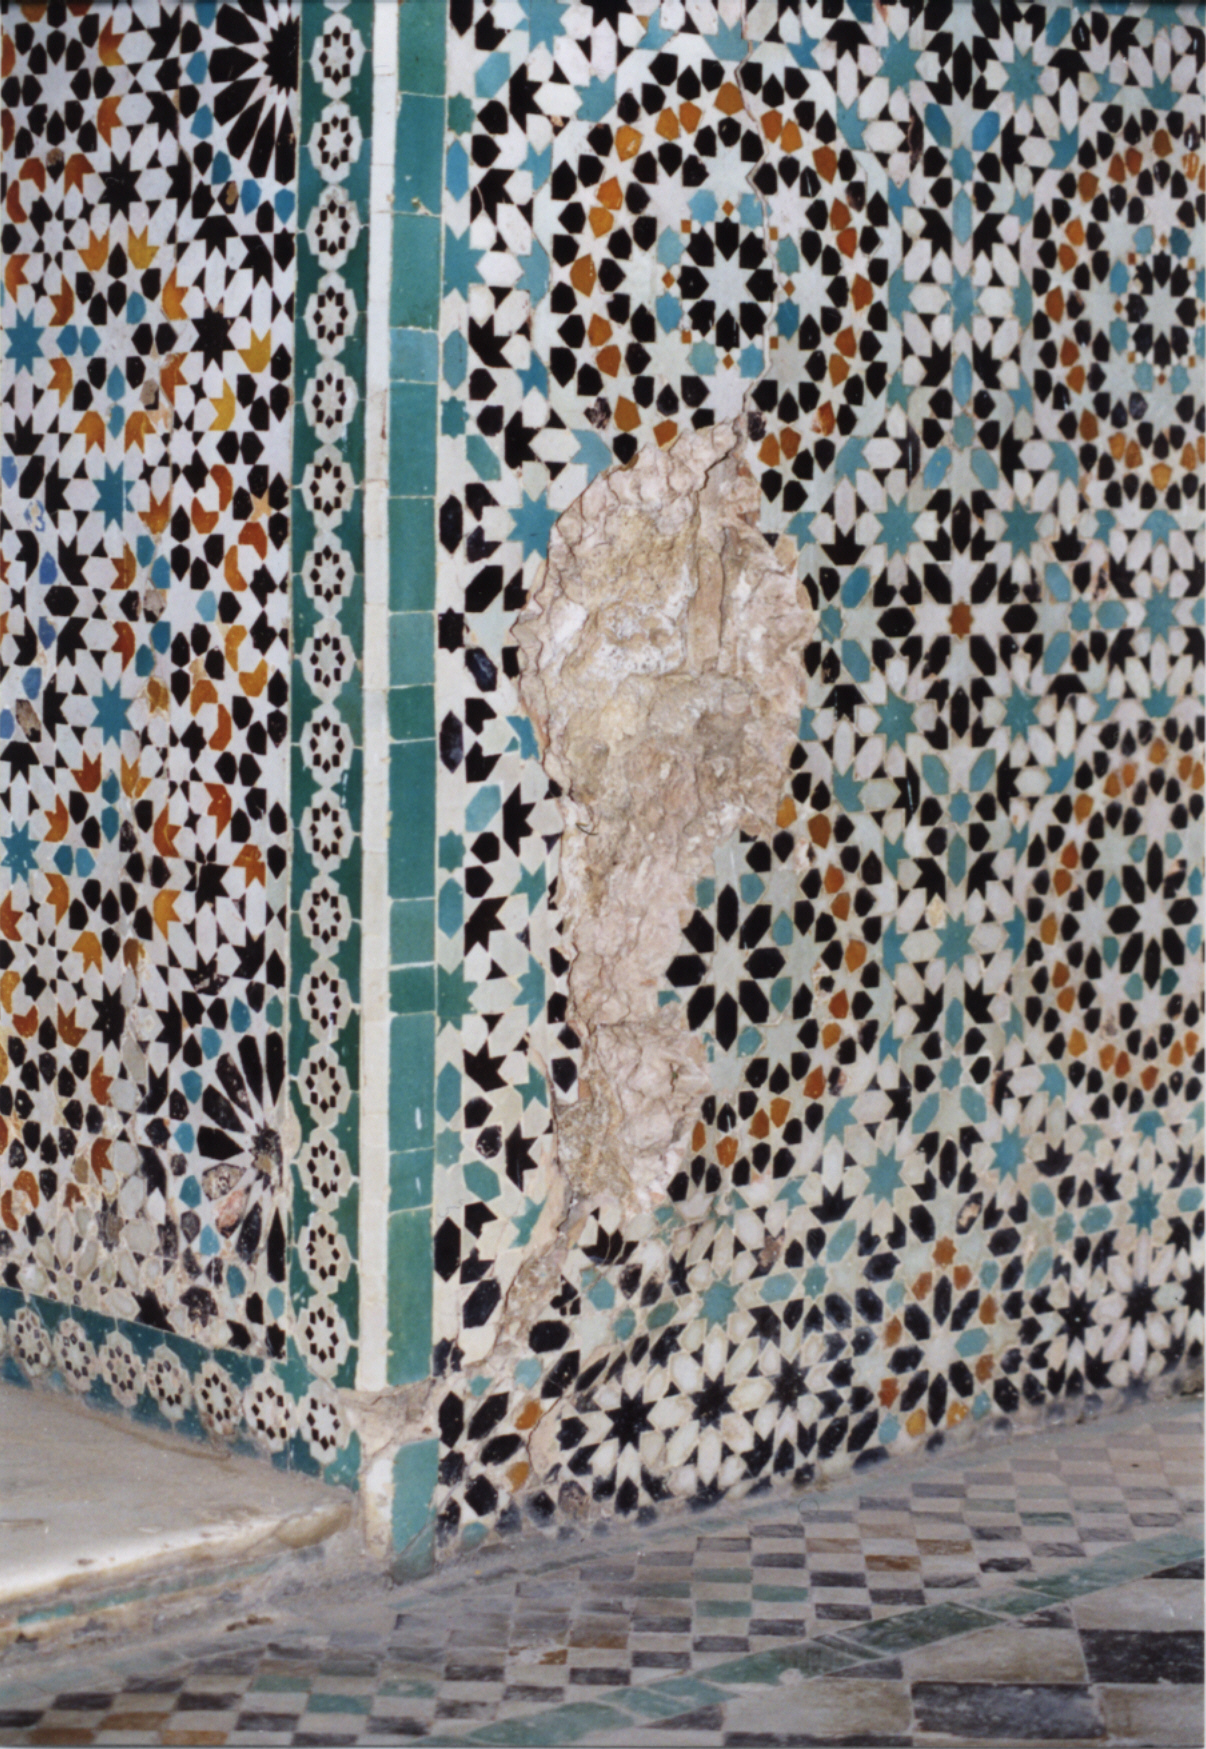
\includegraphics[width=0.45\textwidth]{alteration_1}%
  \quad%
  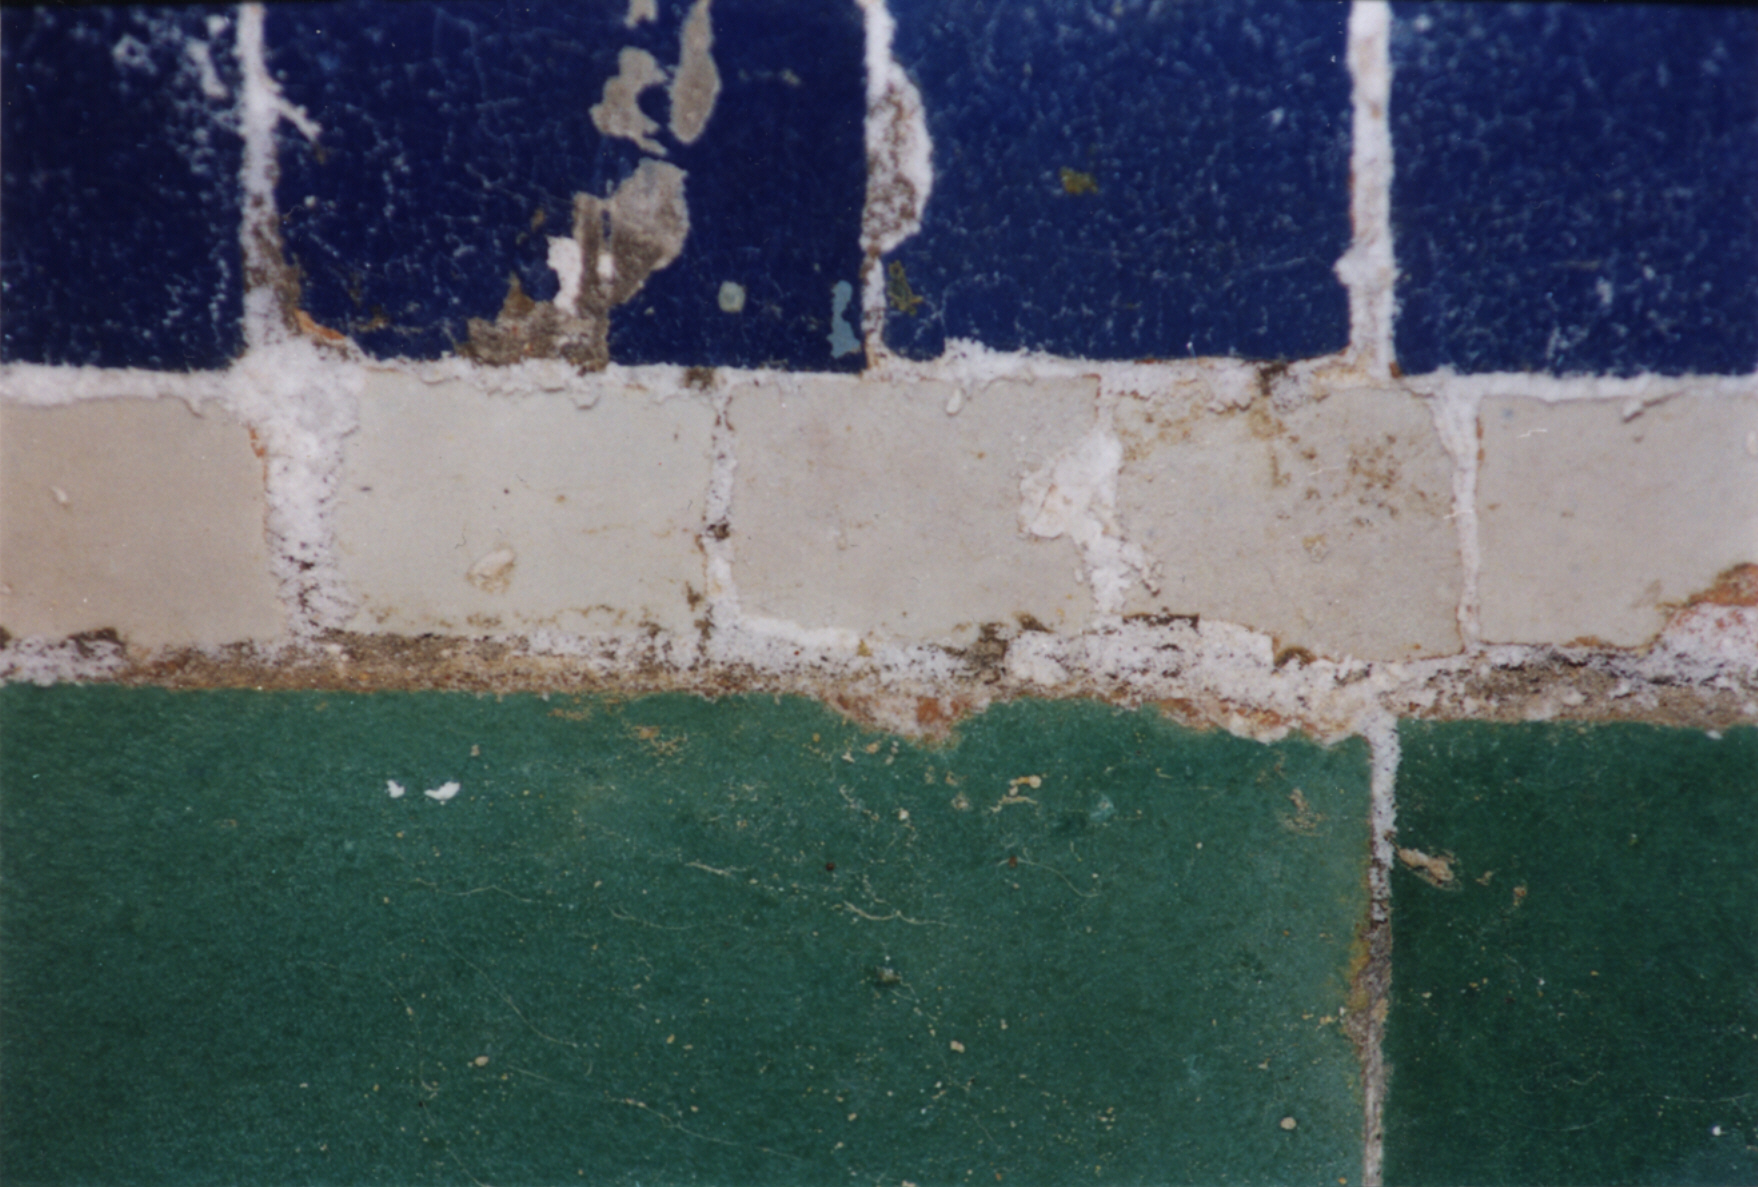
\includegraphics[width=0.45\textwidth]{alteration_2}
  \caption{Différents types d'altération : à gauche, on note un 
           décollement d'une partie du panneau décoré de zelliges ; 
           à droite, des efflorescences salines sont visibles entre 
           les pièces de céramique (clichés :~Schv{\oe}rer, 1999).}
  \label{fig:alteration}
\end{figure}

L'art des zelliges et les bâtiments qu'il décore font partie 
intégrante de la vie et du patrimoine culturel du Maroc. 
Malheureusement, ces témoignages du passé sont aujourd'hui 
victimes des ravages du temps : des panneaux entiers de zelliges 
se détachent, les glaçures sont altérées, on note également la 
présence d'efflorescences salines entre les pièces de céramique
(\fref{fig:alteration}).

Les architectes marocains souhaitent restaurer ces monuments et 
leurs décors de zelliges, en recréant les pièces manquantes selon 
les techniques anciennes, et dans la mesure du possible, mettre en 
{\oe}uvre une politique de conservation préventive. Mais ces 
techniques ne sont pas connues et les artisans actuels se sont 
adaptés aux matériaux modernes et colorants de synthèse.

La problématique de cette étude, portant sur les problèmes de 
préservation des céramiques glaçurées architecturales, s'articule 
donc autour de deux thèmes, dans le but de fournir aux architectes 
les données physico-chimiques nécessaires à leurs travaux : d'une 
part la recherche des techniques de fabrication anciennes, d'autre 
part l'évaluation et la caractérisation des phénomènes d'altération 
rencontrés dans ce type de matériaux.

\chapter{État des connaissances}
%======================================================================

\section{Zelliges}
%----------------------------------------------------------------------

\subsection{Définition}
%~~~~~~~~~~~~~~~~~~~~~~~~~~~~~~~~~~~~~~~~~~~~~~~~~~~~~~~~~~~~~~~~~~~~~~
On appelle \frquote{zellige} un art décoratif basé sur l'assemblage 
de pièces de céramique glaçurée chanfreinées, soigneusement 
découpées, puis assemblées de façon à former des motifs géométriques 
traditionnels. Ce terme désigne également les éléments de céramiques 
elles-mêmes. Les zelliges décorent aussi bien les murs que les sols, 
ou les colonnes des édifices religieux (mosquées, madrasas) et des 
demeures luxueuses.

Ce type de décor est réservé aux parties basses des murs, jusqu'à, 
à peu près, \SI{1.40}{\m} de hauteur. De cette façon, la frise de 
calligraphie, qui borde souvent la partie supérieure des panneaux 
de zelliges, est située à hauteur des yeux. La partie supérieure 
des murs est décorée de stuc sculpté, de boiseries.

Ce revêtement de zelliges est très important aux yeux des marocains 
et offre un contraste étonnant avec la terre battue et la poussière 
des ruelles extérieures. Afin de rester en permanence net et brillant, 
il a toujours fait l'objet des premiers soins de la journée. On 
rapporte que, jusqu'au début du siècle, le maître de maison venant du 
dehors avait coutume de quitter ses babouches au seuil de la cour, 
comme il l'aurait fait à l'entrée d'une mosquée.

\subsection{Historique}
%~~~~~~~~~~~~~~~~~~~~~~~~~~~~~~~~~~~~~~~~~~~~~~~~~~~~~~~~~~~~~~~~~~~~~~
L'origine de l'art des zelliges se situerait en \frquote{Orient}. 
Lors de la conquête du Maghreb et de l'Espagne pendant l'époque 
Omeyyade (\scl{viii}), les Arabes auraient amené avec eux de 
Syrie le principe du décor géométrique \autocite{Damluji_1993a}.

On trouve dans l'est du Maroc, sur des sites Fatimides et Hammadides 
des \sclnum{ix} et \siecle{xi}s (Tunisie et Algérie modernes), des 
décors fait de grands carreaux polychromes de céramique glaçurée, de 
forme géométrique (carreaux de pavement et de parement de la Qal'at 
Ban\=u Hammad). Ces mosaïques seraient inspirées de carreaux de 
céramique Aghlabides et abbassides (\sclnum{viii}-\scl{ix}). Ces 
premiers types de décors auraient ensuite évolué pour donner la 
forme la plus ancienne de zellige à proprement parler : celle des 
minarets almohades et des tours du Maghreb et d'Andalousie des
\sclnum{xii}-\siecle{xiii}s. On peut en voir des exemples 
\incise{motifs blancs et vert turquoise} sur les minarets de la 
Kutubiyya (Mosquée des Librairies) et de la mosquée de la Qasba à 
Marrakech \autocite{Damluji_1993a}.

Les zelliges tels qu'ils sont définis aujourd'hui \incise{très 
petits carreaux monochromes formant une composition polychrome de 
plus de deux couleurs} ne connaîtront de réel essor qu'à la fin du 
\sclnum{xiii} et au début du \siecle{xiv}. C'est sous les Mérinides, 
aux \sclnum{xiv}-\siecle{xv}s, que l'art des zelliges atteint son 
apogée, tant techniquement qu'artistiquement.

En Andalousie, l'industrie zellige sera à cette époque supplantée 
par des imitations peintes sur de grands carreaux polychromes et 
sur d'autres types de carreaux de mosaïque (à reflets métalliques, 
\emph{cuerda seca}, \emph{cuenca}, champlevé). Bien que de tels 
carreaux aient été importés au Maroc et probablement fabriqués 
localement, cette technique ne remplaça pas les zelliges dont la 
tradition sera perpétuée par les Saadiens puis les Alaouites jusqu'à 
nos jours, probablement grâce au repli sur lui-même qui caractérise 
le Maroc à partir du \siecle{xvi} et au conservatisme de sa société 
\autocite{Damluji_1993a}.

On sait peu de choses sur les évolutions stylistiques des zelliges 
à partir du \siecle{xvii}. Ces périodes n'ont, en effet, quasiment
pas été étudiées car elles sont souvent considérées comme la période 
de déclin de l'art des zelliges et donc sans intérêt pour la plupart 
des auteurs.

Certains auteurs \autocite{Castera_1996, Soustiel_1985} mettent en 
avant une seconde hypothèse sur l'origine de la technique zellige. 
Elle aurait été introduite au Maghreb par l'intermédiaire 
d'immigrants espagnols réfugiés en Tunisie pendant la Reconquista 
au \siecle{xiv}. On parle notamment d'un artisan nommé \emph{Qaçim
al-Zalidji} qui aurait donné son nom à cette technique. C'est de là 
que les zelliges auraient été importés au Maroc.

Il est intéressant de noter la ressemblance entre les zelliges 
marocains et les revêtements \emph{qâshânî}, mosaïques de céramique 
glaçurées présentant des motifs floraux, que l'on trouve en Orient, 
à Hérât (Afghanistan) par exemple. De même, le décor géométrique 
n'est pas une spécificité marocaine : au \siecle{xix}, les surfaces 
architecturales de tout l'empire musulman s'en sont couvertes. 
Cependant, l'association, au Maroc, de la technique de la mosaïque 
avec le principe du décor géométrique a aboutit à un véritable art 
abstrait, au sens noble du terme. De plus, sa grande technicité et 
ses qualités artistiques le rendent réellement unique.

\subsection{Technique de fabrication}
%~~~~~~~~~~~~~~~~~~~~~~~~~~~~~~~~~~~~~~~~~~~~~~~~~~~~~~~~~~~~~~~~~~~~~~
Le principal centre de production de zelliges dans le Maroc 
pré-colonial est Fès. Les zelliges présentent ailleurs au Maroc, 
à Meknès, Rabat, Marrakech, Salé, sont, soit importés de cette ville, 
soit produits localement selon sa tradition. Fès a produit depuis 
l'époque médiévale des {\oe}uvres de grande qualité. Il existe 
cependant un deuxième centre de production d'importance, caractérisé 
par une technique de fabrication différente de celle de Fès, du moins 
aux \sclnum{xix}-\siecle{xx}s : Tétouan.

La différence entre ces deux techniques est bien documentée à partir 
de la fin du \siecle{xx}. À Fès, de grands carreaux d'argile sont 
cuits, glaçurés, puis soumis à une seconde cuisson pour fixer le 
mélange glaçurant. Les \emph{f\=urmas} (formes des pièces zellige) 
y sont découpés. Si la technique de Tétouan requiert également deux 
cuissons, les pièces de zelliges sont découpées dans les grands 
carreaux d'argile avant la première. La technique de Fès permet un 
meilleur ajustement des pièces entre elles. En effet, les pièces 
découpées avant la cuisson subissent pendant celle-ci un retrait. 
Néanmoins, la technique de Tétouan est plus facile à mettre en 
{\oe}uvre et les glaçures, plus épaisses, ont la réputation de durer 
plus longtemps et de produire une surface en relief plus attrayante.

Les origines et le développement historique de ces deux techniques 
sont loin d'être clairs. Les premiers exemples de zelliges 
\incise{carreaux monochromes des minarets et tours almohades} furent 
de toute évidence découpés avant la cuisson, à cause de leur taille. 
En revanche, les motifs complexes développés au Maroc sous les 
Mérinides, ainsi qu'en Andalousie (époque nasride) et en Algérie 
(époque zayanide) ont requis l'utilisation de la technique, plus 
précise, de découpe après glaçure. L'apparition, à la fin du Moyen-Âge 
en Espagne, de la technique de découpe avant cuisson est associée un 
appauvrissement de la gamme de compositions de zelliges. Dans le 
Maghreb, cette dernière technique n'est relevée que dans les 
constructions médiévales de Tlemcen et à Tétouan 
\autocite{Erzini_1993a}.

Tétouan étant pratiquement une ville nouvelle, fondée vers 1484 
par des immigrants de Grenade, l'origine de sa technique différente 
pourrait se situer en Espagne musulmane. D'autre part, il semble 
qu'il y ait eu un appauvrissement similaire des compositions zelliges 
au Maroc au début de la période Alaouite et par conséquent, la 
technique de Tétouan pourrait être le résultat d'un déclin général 
\autocite{Erzini_1993b}.

La technique de fabrication actuelle de Fès peut être décomposée en 
différentes étapes.

Tout d'abord, l'argile de \frquote{terre} issue des gisements aux 
alentours de la ville est trempée dans de grands baquets d'eau 
(\emph{zw\={a}b\={\i}}) jusqu'à ce qu'elle ramollisse. 
Elle fermente pendant vingt-quatre heures avant d'être travaillée. 
Le pétrissage amollit la pâte de sorte qu'elle peut être mise dans 
des moules de \SI{1}{\cm} de profondeur qu'on laisse ensuite au soleil 
pendant quatre heures pour que l'eau d'humidité s'évapore. 
Ce procédé, appelé \emph{tans\u{\i}f} ou \emph{ta\u{g}f\={\i}f}, est 
effectué en été et doit fournir un stock de carreaux bruts suffisant 
pour toute l'année. 
Lorsque l'argile est sèche, on procède à la découpe des carreaux de 
zellige à l'aide d'un outil métallique (\emph{al-q\={a}la}).

Une partie des carreaux est alors cuite alors que les autres 
(\emph{mzihr\={\i} nayy}) sont stockés jusqu'à ce qu'on en ait besoin.

Le mélange glaçurant est ensuite appliqué sur les carreaux cuits qui 
subiront une seconde cuisson.

Les couleurs primordiales sont le vert, le bleu, le miel, le blanc 
et le noir, auxquelles s'ajoutent le rouge et différentes nuances 
des couleurs de base. Les pigments proviennent de matériaux locaux.

Les deux cuissons sont menées dans le même four (\emph{far\={\i}na}). 
La partie inférieure du four est réservée aux carreaux séchés au 
soleil, alors que la seconde cuisson se déroule dans la partie 
supérieure. Chaque couleur nécessite une température de cuisson 
spécifique qui détermine sa position dans le four : le blanc et 
le bleu, exigeant une chaleur intense, sont placés tout en bas, le 
rouge et le jaune viennent ensuite, et enfin, on trouve le vert qui 
nécessite le moins de chaleur. Le feu est alimenté avec des noyaux 
d'olive concassés (grignon, déchets solides du broyage des olives).

Après les cuissons, vient le découpage des pièces de zellige 
(\fref{fig:procede_naqs}), à l'aide d'une herminette tranchante 
appelée \emph{manq\={a}\v{s}}. Ce procédé, appelé \emph{naq\v{s}}, 
est selon le \zlaygi (maître zelligeur) \d{H}assan bin 
al-\d{T}ayy\={\i}b al-Haytam\={\i} l'épine dorsale de l'art des 
zelliges, la base pour atteindre la précision.

\begin{figure}[htb]
  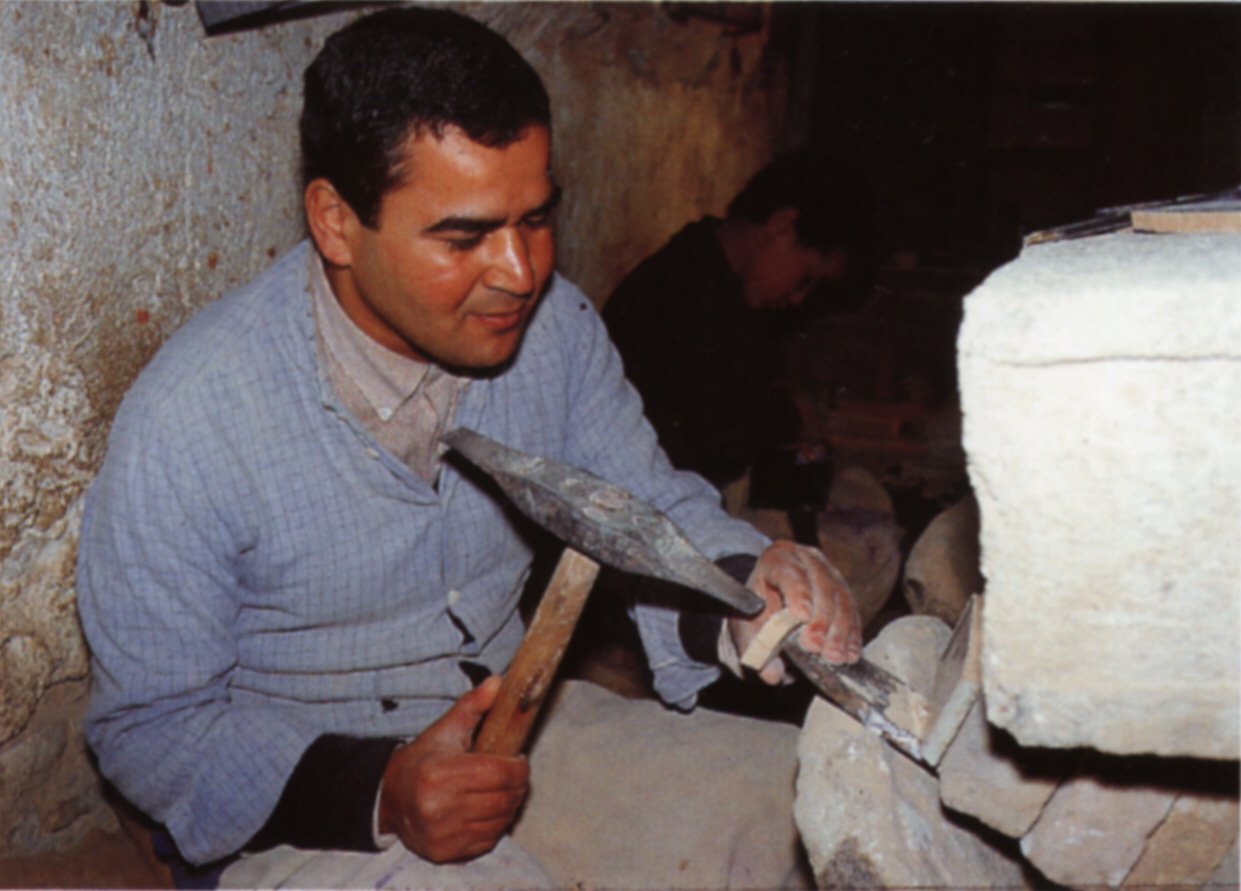
\includegraphics[scale=0.6]{procede_naqs_1}%
  \quad%
  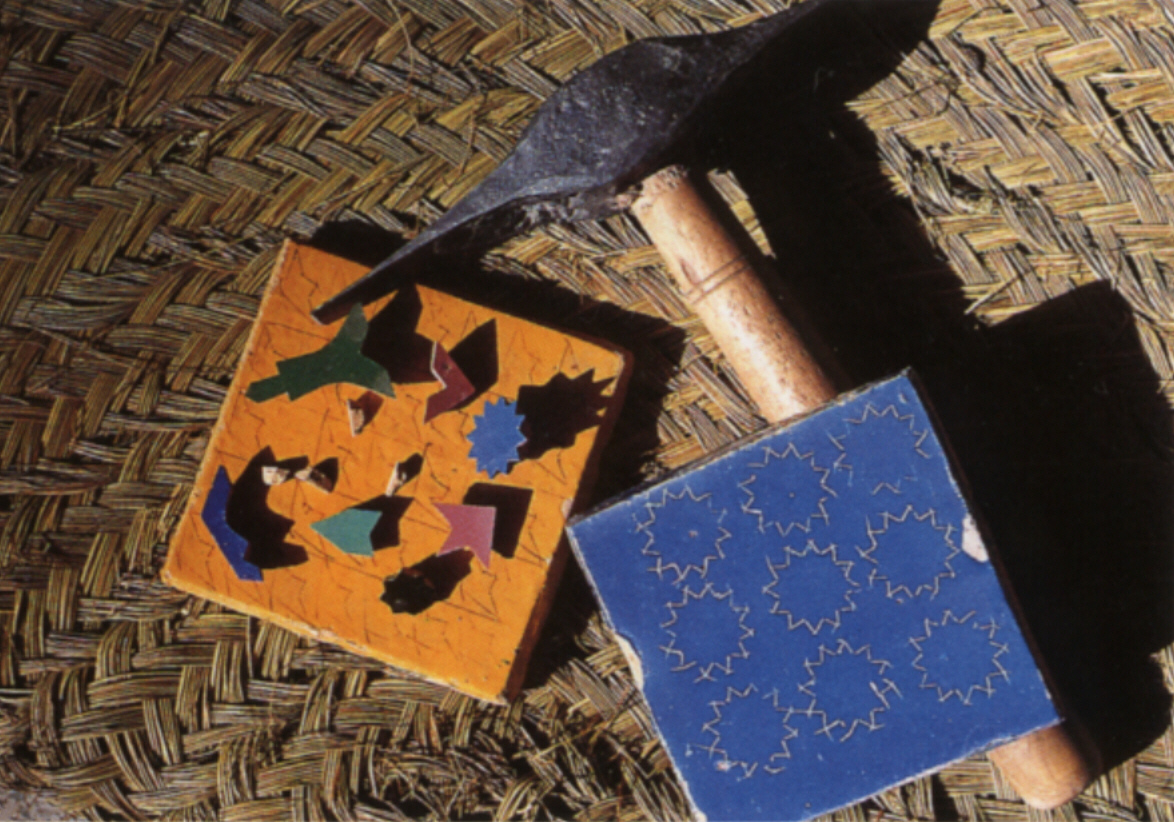
\includegraphics[scale=0.6]{procede_naqs_2}
  \caption[Procédé \emph{naq\v{s}} : découpage des pièces de zellige]
          {Procédé \emph{naq\v{s}} : découpage des pièces de zellige 
           \autocite{Castera_1996}}
  \label{fig:procede_naqs}
\end{figure}

La dernière étape est le \emph{far\v{s}} (\fref{fig:procede_fars}), 
\frquote{processus consistant à étaler les pièces 
\emph{zill\={\i}\u{g}} découpées devant derrière sur le sol selon 
l'agencement ou la composition du motif désigné en tant que partie 
de l'assemblage du panneau final}. \autocite{Damluji_1993a}.
Un premier mortier est utilisé pour souder les pièces entre elles. 
Une \emph{tafr\={\i}\v{s}a} (couche), de \SI{5}{\cm} de profondeur, 
d'un mélange de chaux et de sable est appliqué à l'arrière du panneau 
pour le fixer au mur.

\begin{figure}[htb]
  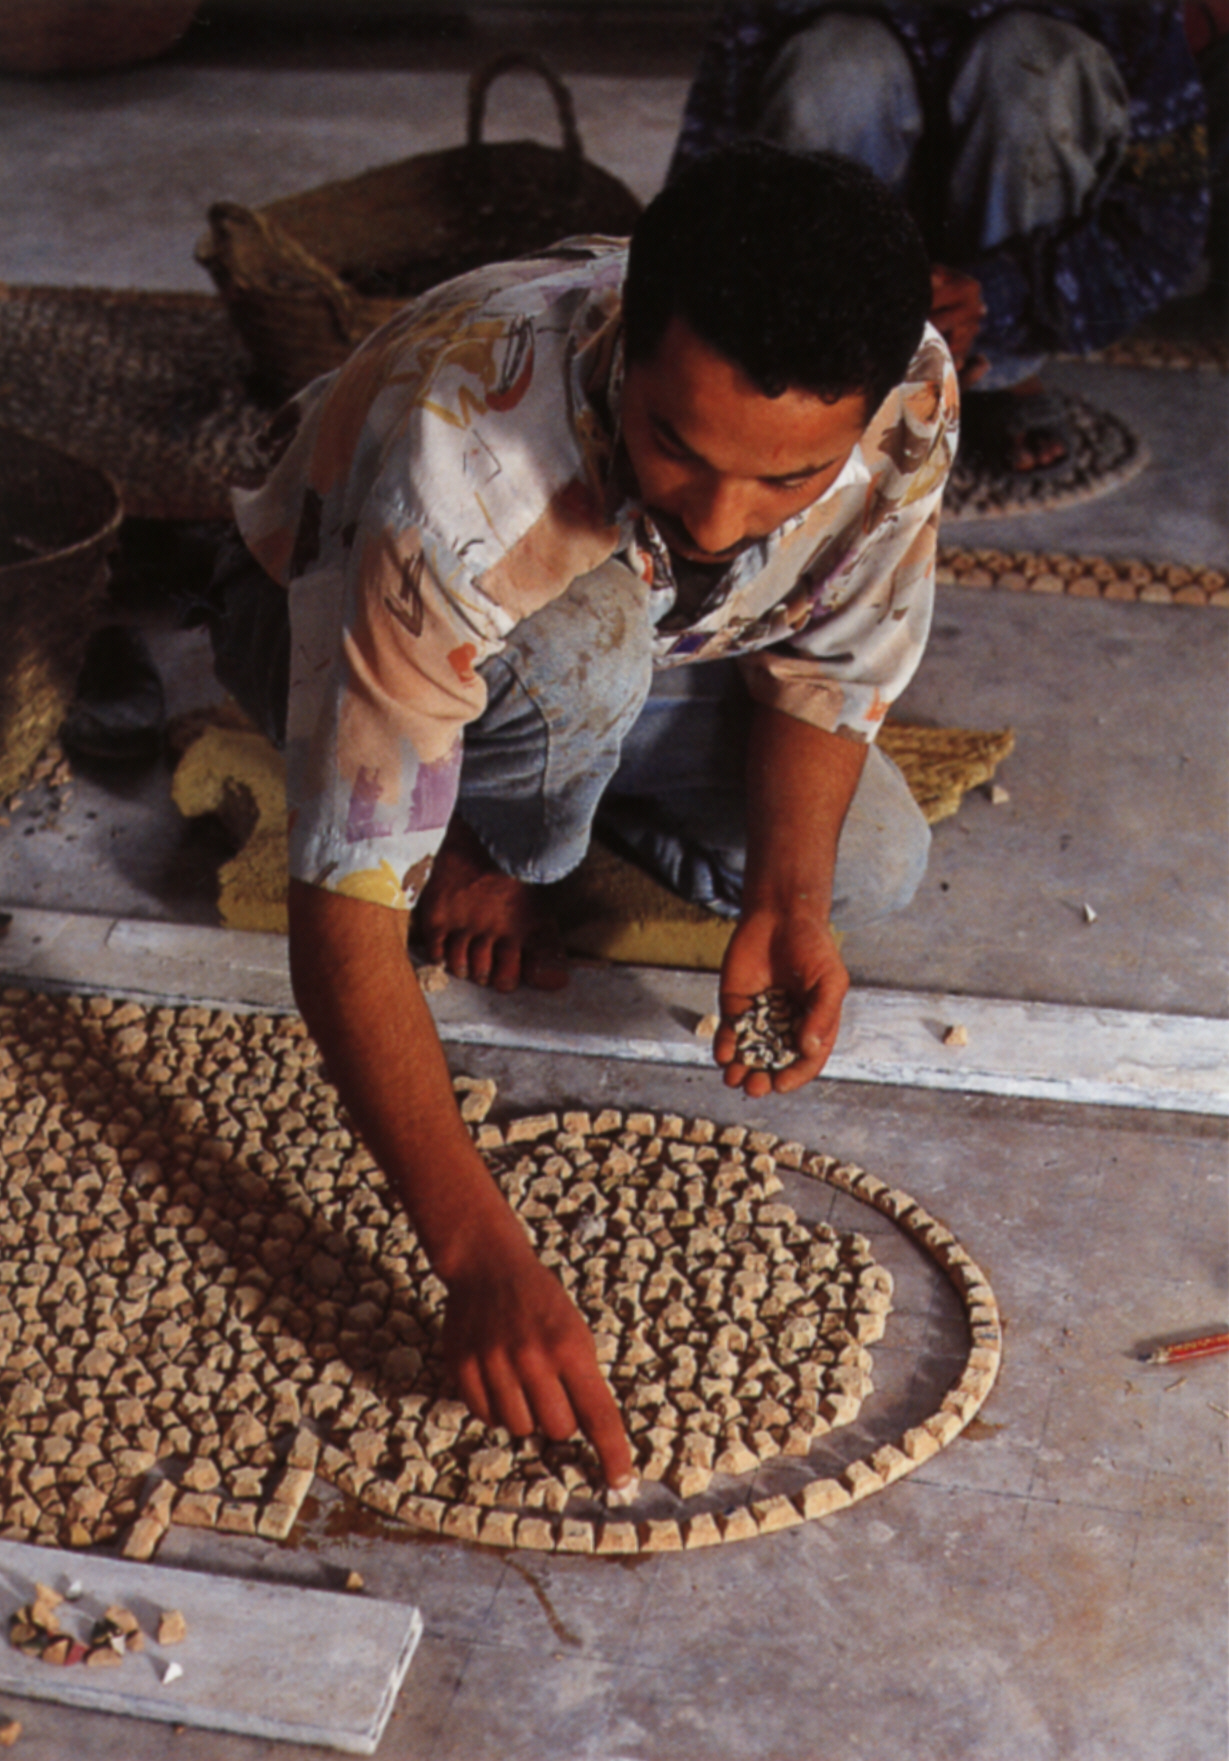
\includegraphics[scale=0.6]{procede_fars}%
  \caption{Procédé \emph{far\v{s}} : assemblage des pièces 
           \autocite{Castera_1996}.}
  \label{fig:procede_fars}
\end{figure}

% \begin{sidecaption}
%       [Procédé \emph{far\v{s}} : assemblage des pièces]
%       {Procédé \emph{far\v{s}} : assemblage des pièces 
%        \autocite{Castera_1996}.}
%       [fig:procede_fars]
%   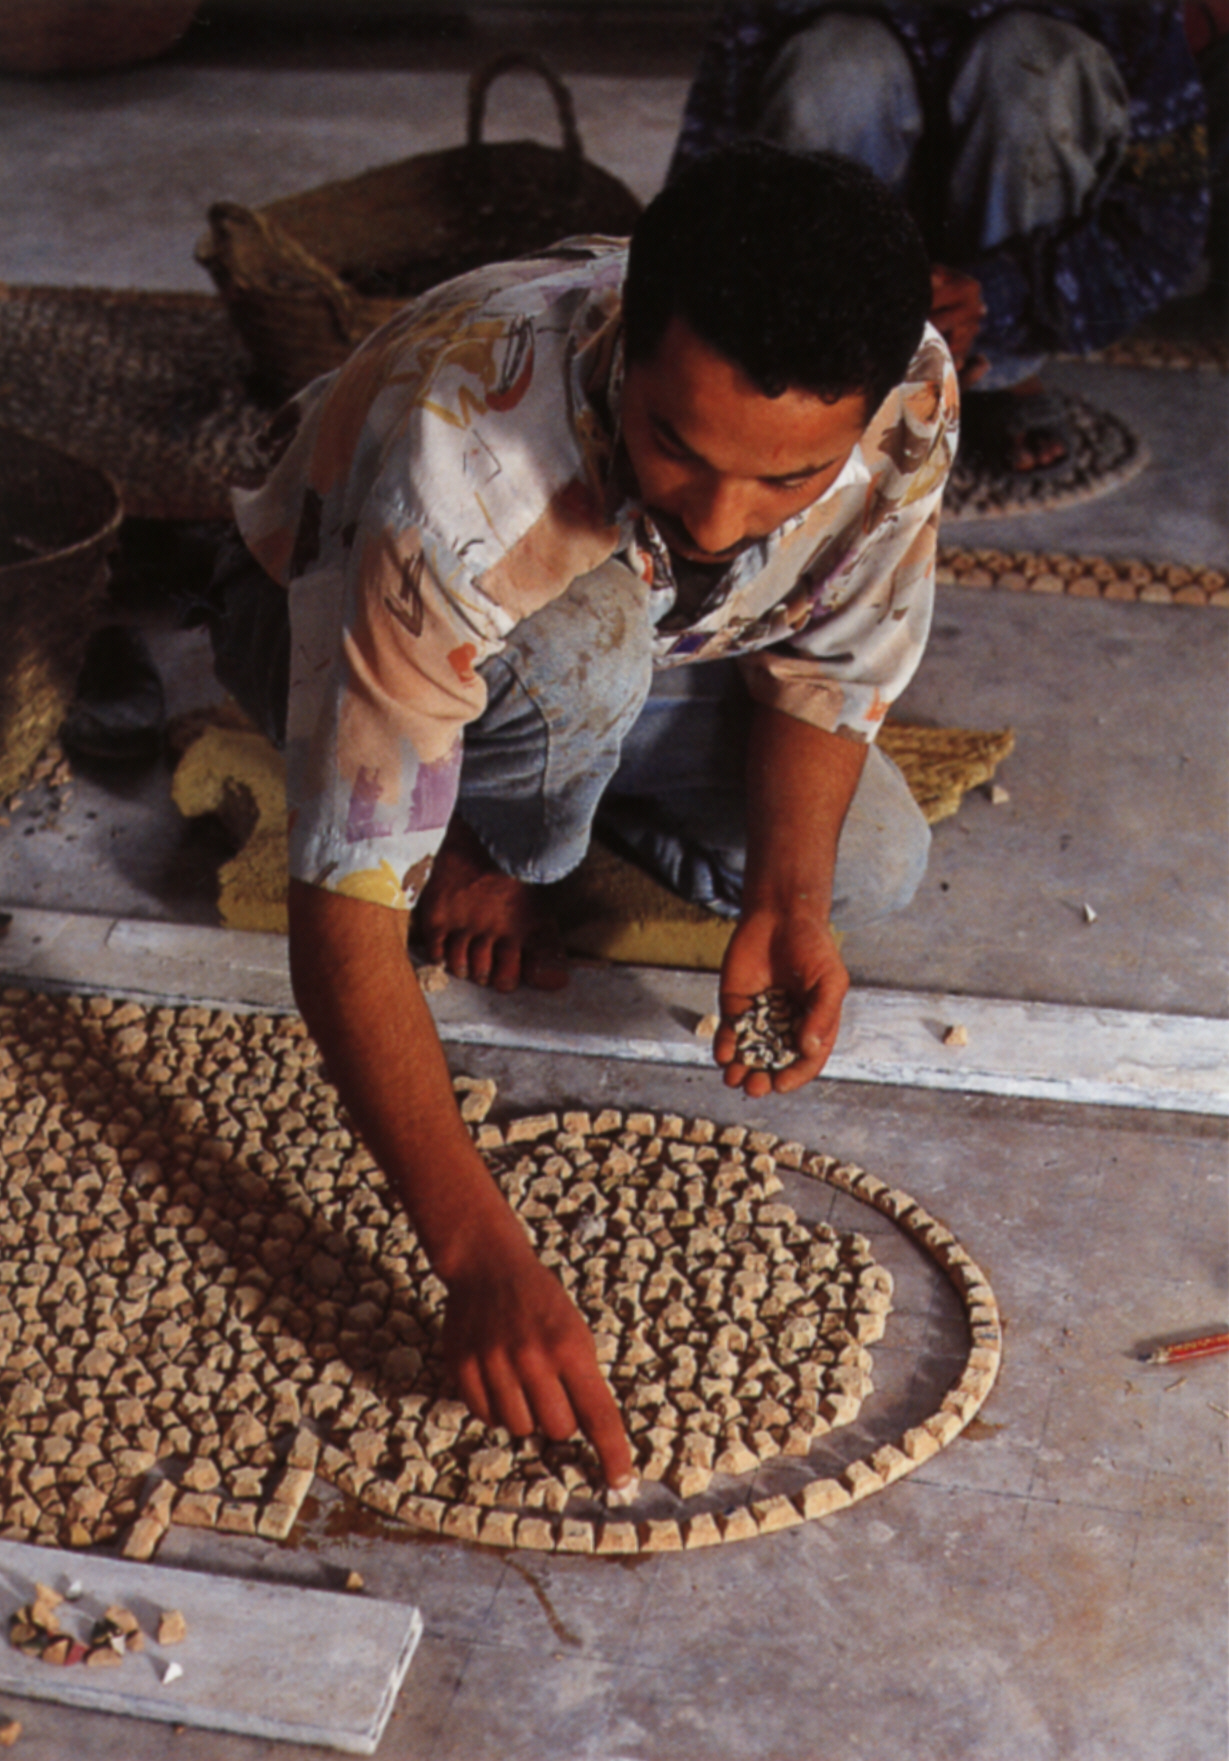
\includegraphics[scale=0.6]{procede_fars}%
% \end{sidecaption}

L'art des zelliges nécessite un apprentissage très long. Il faut 
passer par toutes les étapes du métier, des plus ingrates aux plus 
valorisantes, avant de devenir un \emph{maallem}, un maître-artisan. 
Al-Haytam\={\i}, soixante-cinq ans, est rentré dans le métier à l'âge 
de douze ans. Il passa d'abord sept ans comme apprenti, à dessiner 
les \emph{f\={u}rmas} et les compositions de zelliges, à apprendre 
le mesurage et les divisions géométriques qui leur sont liés. Il 
lui fallut vingt-et-un ans de plus pour maîtriser le découpage et 
l'équarrissage des pièces. Depuis, il se consacre à la fabrication 
de zelliges, au découpage et à la disposition des panneaux et à leur 
transport sur le site d'assemblage.

\subsection{Étude symbolique et géométrique}
%~~~~~~~~~~~~~~~~~~~~~~~~~~~~~~~~~~~~~~~~~~~~~~~~~~~~~~~~~~~~~~~~~~~~~~
Les trois genres de l'art islamique liés à l'architecture sont le 
décor calligraphique, l'arabesque florale et le décor géométrique. 
Toutes les écritures ont donné naissance à un art de la calligraphie. 
De même, des formes décoratives similaires à l'arabesque florale se 
sont développées dans d'autres civilisations : les enluminures 
moyenâgeuses ou les entrelacs celtiques par exemple. Le décor 
géométrique, en revanche, est une invention majeure de l'art 
islamique. Et c'est au Maroc et en Andalousie, à travers l'art des 
zelliges, que son développement fut le plus exceptionnel.

L'essor du décor géométrique est certainement lié à la limitation 
de la figuration imposée par la religion. En effet, si les images 
ne sont pas prohibées par le Coran, les \emph{Haddiths} 
\incise{commentaires ajoutés au Livre Saint au \siecle{ix}} 
proscrivent celles portant une ombre (statuaire, modelé en peinture, 
perspective). Ceci rendra possible le développement de la miniature 
aux \sclnum{xiii}-\siecle{xiv}s mais l'interdiction est totale dans 
les mosquées et les corans enluminés \autocite{Castera_1996}.

On peut rapprocher le décor géométrique islamique des traditions 
artistiques de sociétés primitives qui ont utilisé des symétries 
portant sur des formes géométriques simples. L'enracinement de l'art 
islamique dans ces formes et concepts archaïques lui donne une portée 
universelle. Son génie fut de développer un langage d'une richesse et 
d'une puissance d'expression extraordinaire. Dans ce type de décor, 
il n'y a plus de distinction fond-forme, les formes simples sont 
assemblées sans vide ni recouvrement. Seule la couleur impose au 
regard une interprétation plutôt qu'une autre \autocite{Castera_1996}.

L'art des zelliges est une image de la représentation islamique 
du monde. Il contient plusieurs niveaux de signification à la fois 
artistiques et scientifiques dont on ne peut saisir totalement le 
sens en quelques jours, quelques mois ou même quelques années d'étude.

Selon le \emph{maallem} A\d{h}mad D\={\i}b, seuls deux facteurs sont 
à prendre en compte pour comprendre cet art : d'une part, la pratique 
et la mémorisation du Livre Saint, base de son {\oe}uvre, de sa 
signification, de sa puissance ; d'autre part, la discipline 
d'apprentissage par c{\oe}ur qui est la base du talent visuel et 
manuel.

En fait, les maîtres-artisans pensent que leur art est une inspiration 
divine, Dieu est l'auteur suprême.

L'art des zelliges répond à certains principes de bases : les règles 
de proportions ne dépendent pas de codes empiriques traditionnels mais 
de nécessités purement géométriques ; le cadre arbitraire du motif ne 
doit être qu'une fenêtre ouverte sur un paysage abstrait qui reproduit 
à l'infini la même figure. La monotonie qui risquerait d'en découler 
est brisée par les imperfections résultant de la réalisation manuelle.

La \emph{f\={u}rma} de base est le \hatim (\fref{fig:furmas}), 
octogone étoilé ou sceau de Salomon. Toutes les autres 
\emph{f\={u}rma} en sont dérivées. Il est aussi le point de départ 
pour la division d'un motif et d'un panneau mural. Son axe est en 
quelque sorte le centre de gravité de la composition. Un \zlaygi 
confie : \frquote{Lorsque nous ajustons le positionnement du 
\emph{hamnisi} (motif étoilé à cinquante branches), nous nous servons 
du \emph{dabid} (compas à pointe sèche) pour produire un cercle 
parfait, en localisant le \hatim au centre : ceci nous donne la 
mesure, que ce soit un mètre ou deux, cent ou mille.} 
\autocite{Castera_1996}.

\begin{figure}[htb]
  \begin{tikzpicture}
    \node at ( 0.00, 0.00) 
          {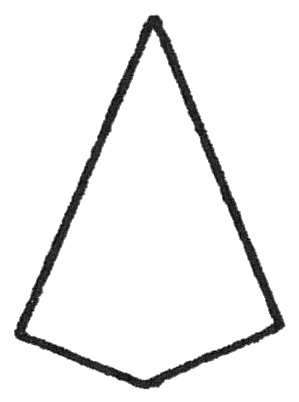
\includegraphics[scale=1]{furmas_luza}} ;
    \node at ( 0.00, 5.00) 
          {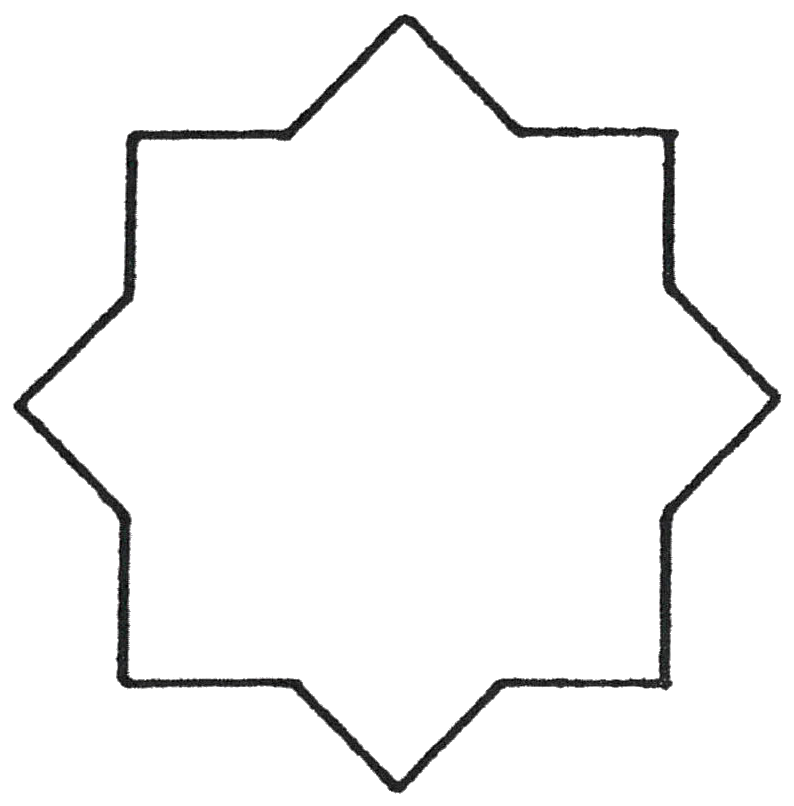
\includegraphics[scale=1]{furmas_hatim}} ;
    \node at (-3.00, 2.00) 
          {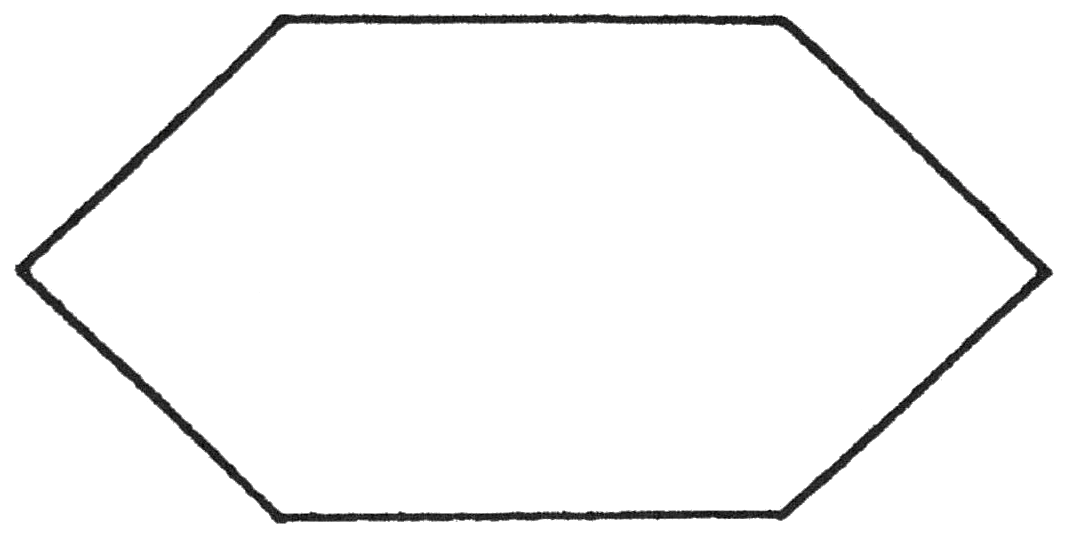
\includegraphics[scale=1]{furmas_saft}} ;
    \node at ( 3.00, 2.00) 
          {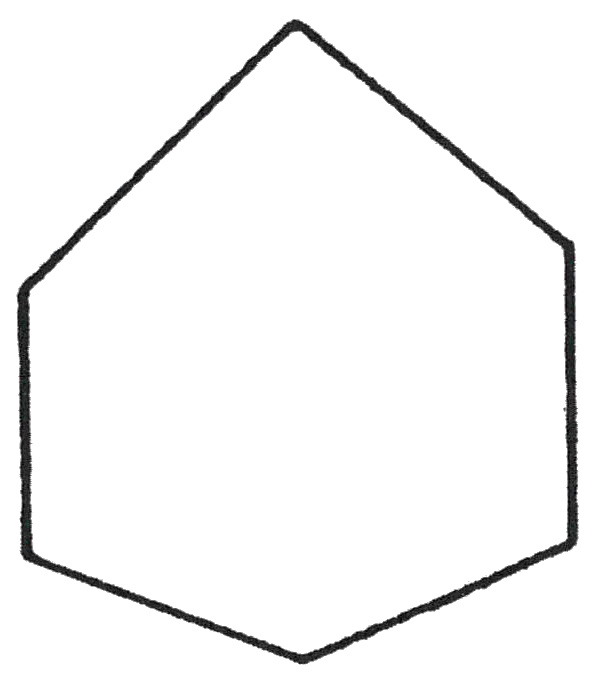
\includegraphics[scale=1]{furmas_kwayra}} ;
    \node at (-2.50,-2.00) 
          {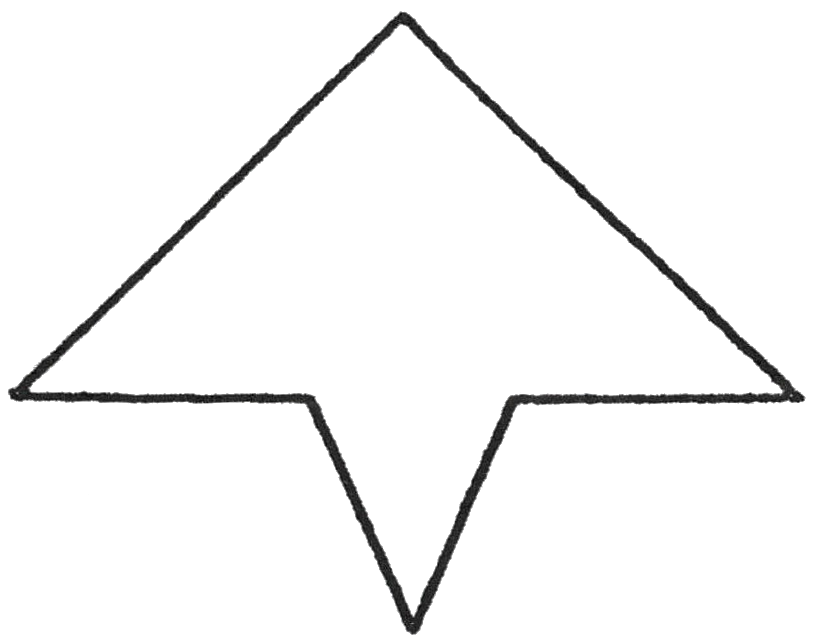
\includegraphics[scale=1]{furmas_hattayfa}} ;
    \node at ( 2.50,-2.00) 
          {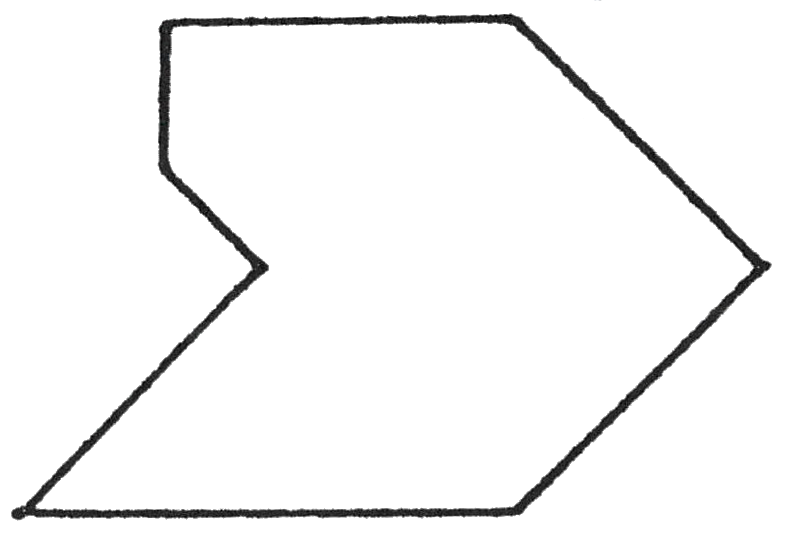
\includegraphics[scale=1]{furmas_fawrkat}} ;
  \end{tikzpicture}
  \caption{Différentes f\={u}rmas de zelliges \autocite{Castera_1996}.}
  \label{fig:furmas}
\end{figure}

Sa construction s'inscrit dans un cercle, forme parfaite par 
excellence, flanqué de quatre autres, tous identiques 
\fref{fig:cercle}. Cette figure symbolise pour Keith~\bsc{Critchlow} 
et Paul~\bsc{Marchant} les quatre coins du temps et de l'espace, à 
travers le cycle du soleil ou celui de la lune. Le cercle central 
représente le cycle complet et les quatre cercles adjacents sont 
l'image des quatre phases (solstices et équinoxes ou pleine lune, 
nouvelle lune, premier et dernier quartier).

\begin{figure}[htb]
  \begin{tikzpicture}[scale=2]
    \clip ( 0.00, 0.00) circle (2.3) ;

    \draw [dashed] ( 0.00, 0.00) circle (1) ;

    \draw [loosely dashdotted] plot(\x, \x) ;
    \draw [loosely dashdotted] plot(\x,-\x) ;
    \draw [loosely dashdotted] plot(\x,0) ;
    \draw [loosely dashdotted] plot(0,\x) ;

    \draw ( 1.00, 0.00) circle (1) ;
    \draw ( 0.00, 1.00) circle (1) ;
    \draw (-1.00, 0.00) circle (1) ;
    \draw ( 0.00,-1.00) circle (1) ;

    \draw [thick] \drawhatim ;
  \end{tikzpicture}
  \caption{Les cinq cercles dans lesquels s'inscrit le \hatim 
           \autocite{Castera_1996}.{}}
  \label{fig:cercle}
\end{figure}

On peut considérer que la plupart des motifs sont construits à 
partir de structures polygonales où alternent deux pièces 
essentielles, le \hatim et le \emph{\d{s}aft}. Une telle structure 
est le \frquote{squelette} (\fref{fig:squelette}) du motif qui 
apparaît quand les lignes courant vers l'intérieur se rejoignent 
en respectant les symétries de l'ensemble. On appelle cela la 
\frquote{résolution} du squelette On peut \frquote{déguiser} ces 
squelettes de sorte qu'ils ne soient pas directement discernables, 
ou même les éliminer totalement du motif. Les squelettes basés sur 
l'octogone sont les plus spécifiques du Maroc et les plus représentés 
dans son architecture. Ces squelettes, une fois habillés, sont 
associés en motifs périodiques. Comme la plupart des figures 
polygonales utilisées ne permettent pas de couvrir entièrement une 
surface plane, il faudra leur associer une ou plusieurs autres figures 
limitées par de nouveaux squelettes. De nouveaux motifs seront ainsi 
créés et ce processus est quasiment sans fin.

\begin{figure}[htb]

  \begin{minipage}[b]{0.33\textwidth}
    \centerfloat
    \begin{tikzpicture}[thick, fill=white, scale=0.4]
      \squelettea
      \fill (-2,-2) rectangle (2,2) ;
    \end{tikzpicture}
    \subcaption{\label{fig:squel_a1}}
  \end{minipage}%
  \quad
  \begin{minipage}[b]{0.33\textwidth}
    \centerfloat
    \begin{tikzpicture}[thick, fill=white, scale=0.4]
      \squelettea
      \filldraw \drawhatim ;
    \end{tikzpicture}
    \subcaption{\label{fig:squel_a2}}
  \end{minipage}%
  \quad
  \begin{minipage}[b]{0.33\textwidth}
    \centerfloat
    \begin{tikzpicture}[thick, fill=white, scale=0.4]
      \squelettea
      \fill (-1,-1) rectangle (1,1) ;
      \foreach \x in {0, 90, 180, 270} {%
        \draw [rotate=\x]
              ( {1-sqrt(2)} ,  1 )          -- 
              ( {1-sqrt(2)} , {sqrt(2)-1} ) -- 
              ( -1 , {sqrt(2)-1} ) ;
      }
    \end{tikzpicture}
    \subcaption{\label{fig:squel_a3}}
  \end{minipage}%

  \bigskip

  \begin{minipage}[b]{0.33\textwidth}
    \centerfloat
    \begin{tikzpicture}[thick, fill=white, scale=0.4]
      \squeletteb
      \fill (-0.5, 1) -- (-2.5,-1) -- 
            (0.5, -1) -- ( 2.5, 1) -- cycle ;
    \end{tikzpicture}%
    \subcaption{\label{fig:squel_b1}}
  \end{minipage}%
  \quad%
  \begin{minipage}[b]{0.33\textwidth}
    \centerfloat
    \begin{tikzpicture}[thick, fill=white, scale=0.4]
      \squeletteb
    \end{tikzpicture}
    \subcaption{\label{fig:squel_b2}}
  \end{minipage}%

  \caption{\subcaptionref{fig:squel_a1} et 
           \subcaptionref{fig:squel_b1} : différents squelettes ; 
           \subcaptionref{fig:squel_a2}, \subcaptionref{fig:squel_a3}, 
           \subcaptionref{fig:squel_b2} : diverses résolutions des 
           squelettes \autocite{Castera_1996}.}
  \label{fig:squelette}
\end{figure}

Les motifs de zelliges présentent des symétries intéressantes : on 
peut considérer un triangle minimal de base (\fref{fig:sym_triangle}) 
qui permet, par des symétries axiales (\fref{fig:sym_triangle} et 
\fref{fig:sym_dessin}) de reconstituer l'ensemble du motif 
(\fref{fig:sym_complet}).


\begin{figure}[htb]
  \begin{minipage}[b]{0.45\textwidth}
    \centerfloat
    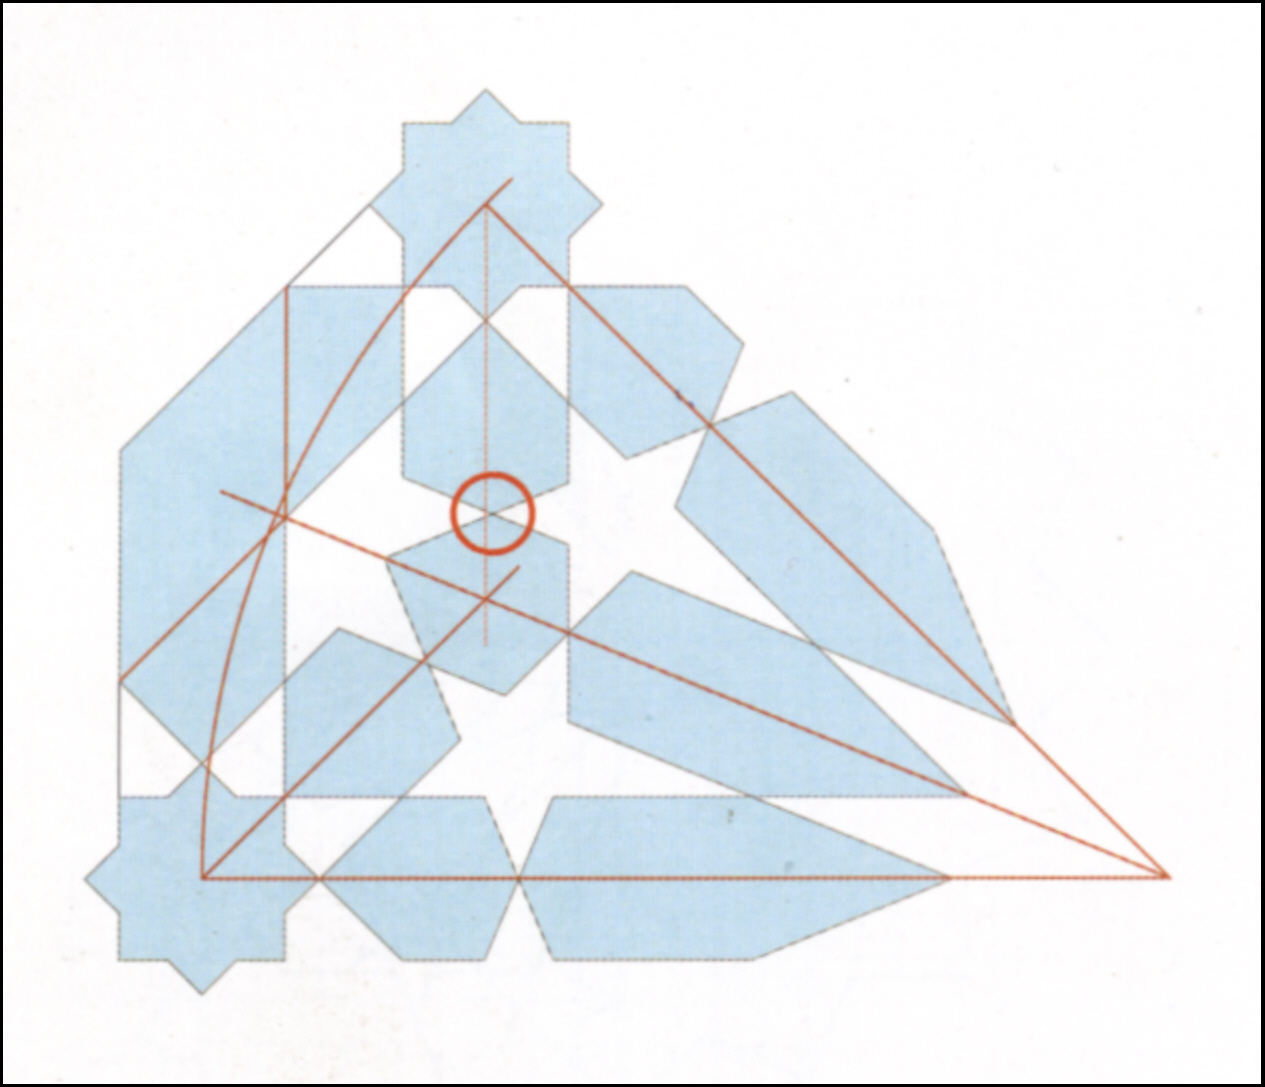
\includegraphics[width=\textwidth]{symetrie_motif_base_ori}
    \subcaption{Triangle minimal 
                \label{fig:sym_triangle}}
  \end{minipage}%

  \bigskip

  \begin{minipage}[b]{0.45\textwidth}
    \centerfloat
    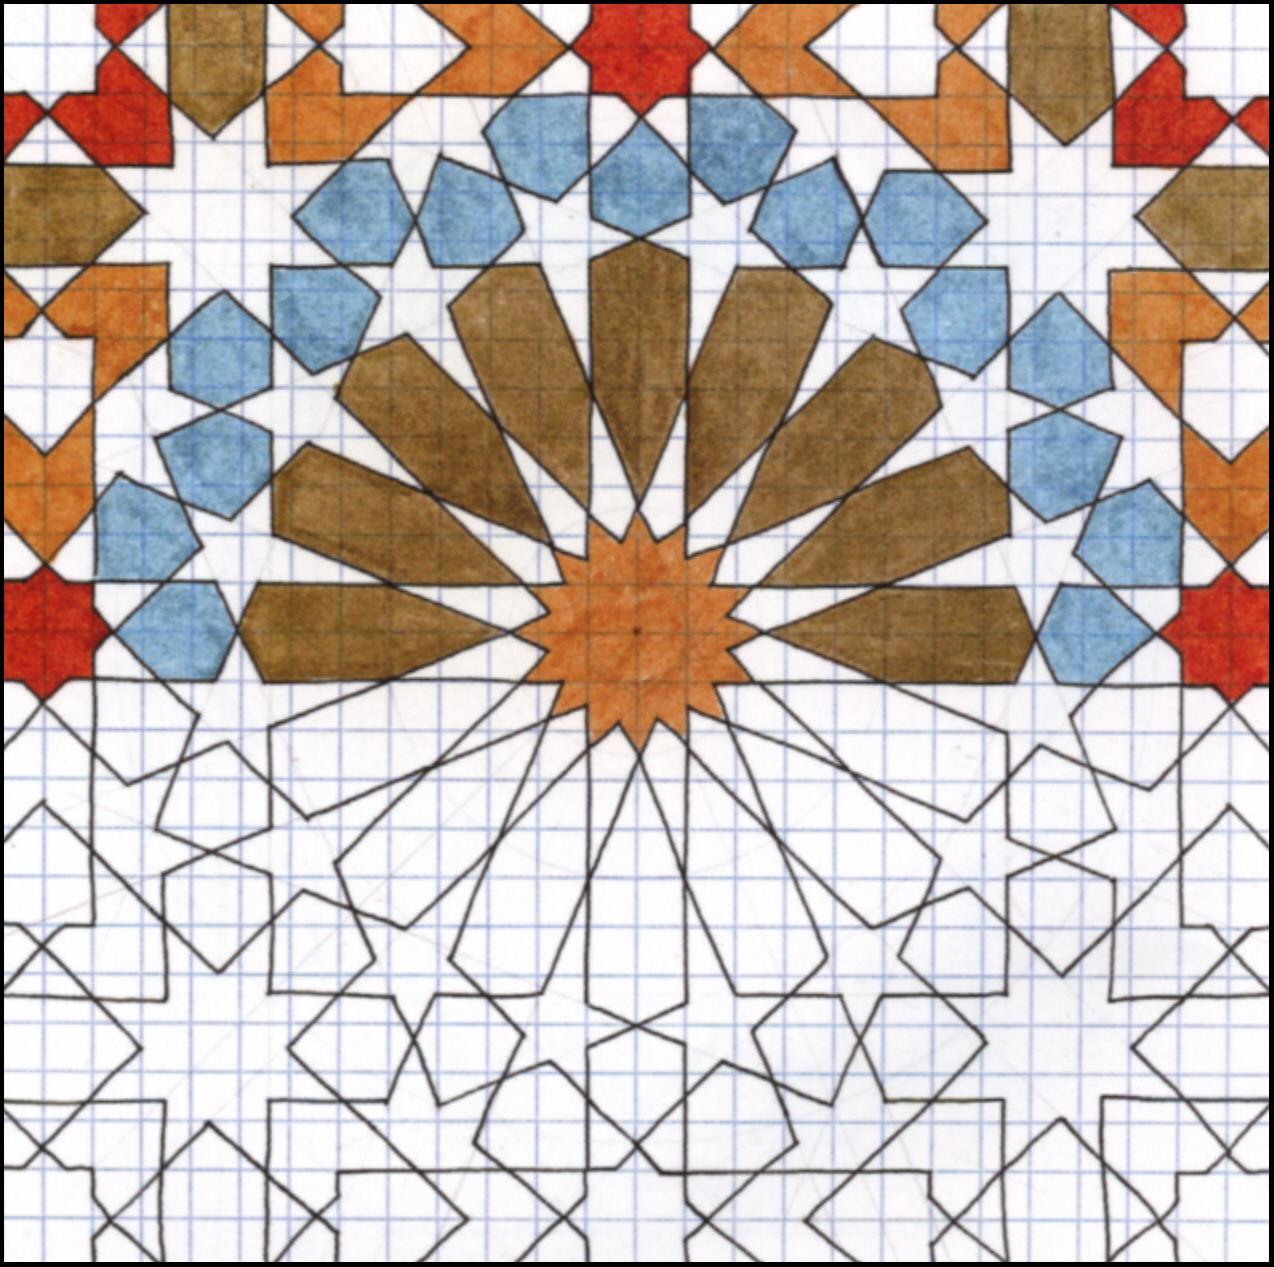
\includegraphics[width=\textwidth]{symetrie_motif_dessin}
    \subcaption{Construction du motif par symétries 
                \label{fig:sym_dessin}}
  \end{minipage}%
  \quad
  \begin{minipage}[b]{0.45\textwidth}
    \centerfloat
    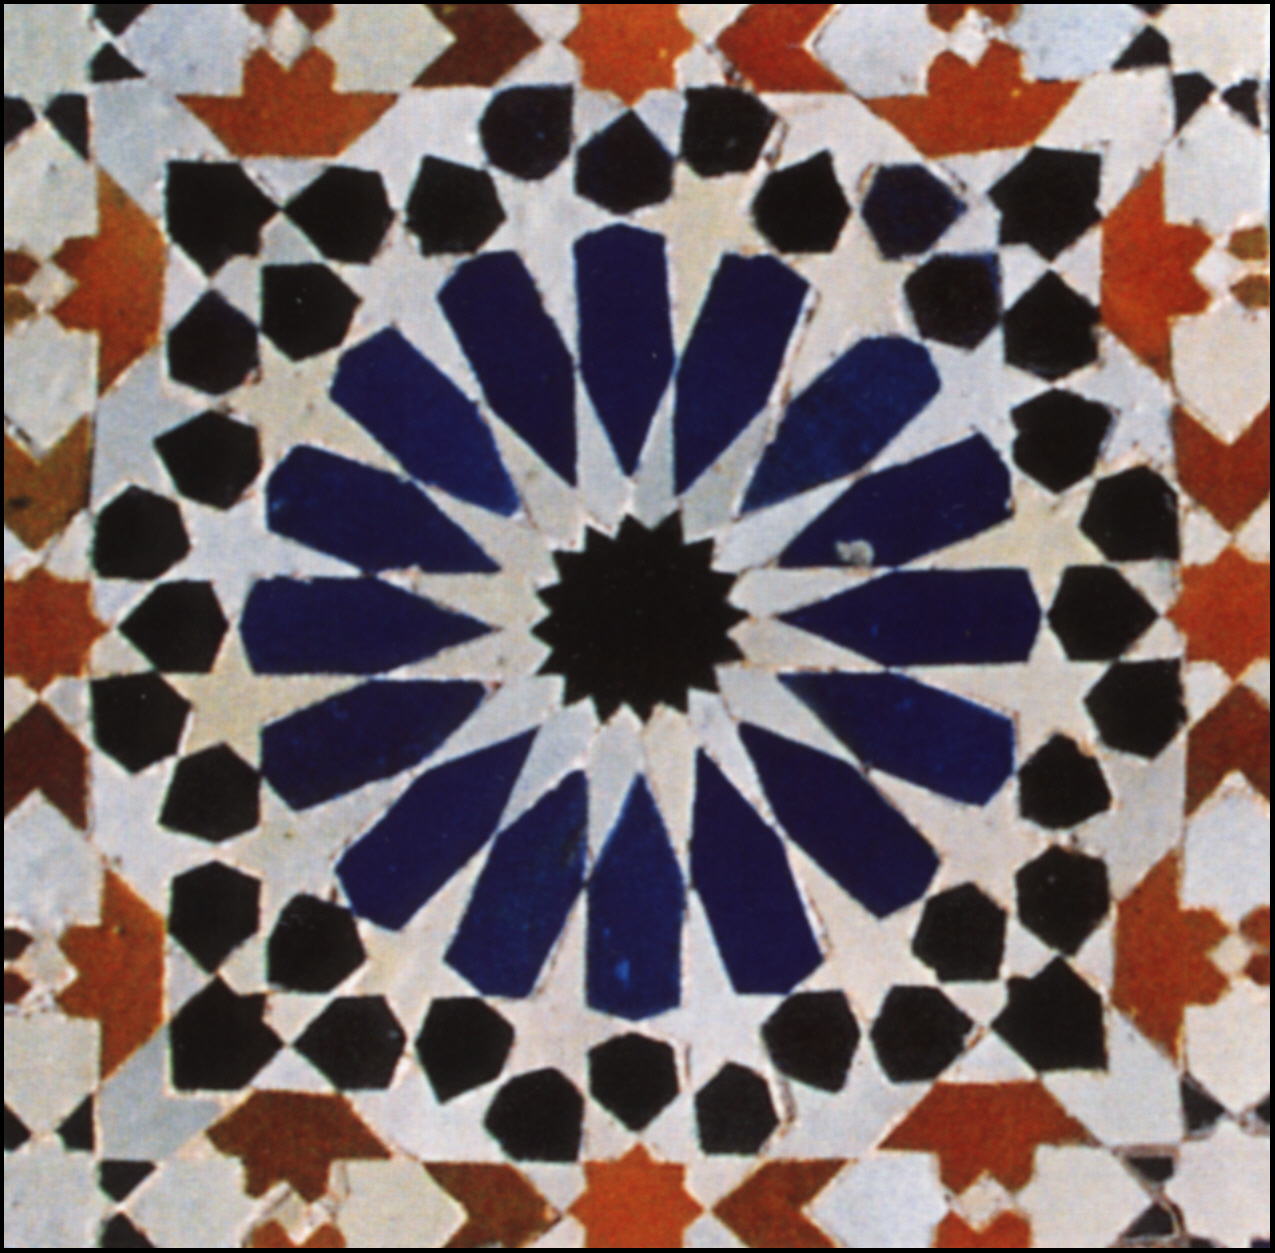
\includegraphics[width=\textwidth]{symetrie_motif_complet}
    \subcaption{Motif complet 
                \label{fig:sym_complet}}
  \end{minipage}
  \caption{Symétrie des motifs de zelliges \autocite{Castera_1996}.}
  \label{fig:symetrie}
\end{figure}

\section{Données physico-chimiques}
%----------------------------------------------------------------------

Les recherches bibliographiques préliminaires à l'étude au laboratoire 
ont permis de mettre en relief le manque de données physico-chimiques 
sur les zelliges.

Cependant, les zelliges sont en fait des pièces de céramique glaçurée, 
matériau étudié depuis de nombreuses années au CRPAA ainsi que dans 
d'autres laboratoires, et ayant fait l'objet de plusieurs publications 
% \autocite{Schvoerer_1998 ; Delvert_1991} 
et thèses 
\autocite{Rafaillac_1994}.

\chapter{Objectifs}
%======================================================================

Nous nous sommes fixé comme objectif principal pour cette étude, la 
recherche des technologies de fabrication anciennes. Ceci passe par 
une caractérisation physico-chimique de la céramique glaçurée. Elle 
se décompose en :

\begin{itemize}
\item La détermination des agents chromogènes responsables de la 
      couleur de la glaçure ;
\item Le calcul des coordonnées trichromatiques (qui donnent une 
      mesure objective de la couleur) ;
\item L'étude de la texture de la glaçure et du support céramique ;
\item La détermination des compositions élémentaires (glaçure et 
      terre cuite) ;
\item La détermination de la composition cristallographique de la 
      terre cuite.
\end{itemize}

Un deuxième objectif important est l'évaluation de l'état de 
conservation des échantillons et, le cas échéant, l'étude de leur 
altération.

Il sera également intéressant de réaliser une étude comparative 
entre les différents travaux menés en parallèle sur les zelliges au 
laboratoire, pour essayer d'en tirer des indices sur l'évolution 
chronologique et les différences géographiques de la technique des 
zelliges.

Enfin, les zelliges étant un sujet nouveau au laboratoire, il est 
particulièrement important de mettre en place une base de données, 
tant bibliographique que physico-chimique, sur ce matériau.


\part{Matériel et méthodologie}
%!TEX root = MemoireZelliges_simple.tex

\chapter{Présentation des échantillons}
%======================================================================

Les cinq échantillons que j'ai étudiés pendant mon stage au CRPAA 
proviennent du \PaM, daté du \siecle{xvii} et situé dans Meknès, 
la Versailles du Maroc.

\section{Meknès, capitale de Moulay Ismaïl}
%----------------------------------------------------------------------

Meknès (\fref{fig:maroc}) est la Cité Impériale de Moulay Ismaïl, 
second sultan de la dynastie alaouite. Lorsqu'il monta sur le trône 
en 1672, il en fit sa capitale et y entreprit des travaux de grande 
envergure pour en faire l'égal de Versailles qu'il admirait. 
L'ancienne casbah mérinide fut rasée pour faire place à des monuments 
grandioses, palais, mosquées, casbah, greniers et jardins, à l'abri 
derrière plus de quarante kilomètres d'un triple rempart de pierre. 
La mort de Moulay Ismaïl en 1727 et les guerres de succession qui 
en découlèrent mirent un terme prématuré aux travaux. Il perdit 
rapidement son rôle de résidence royale et Fès redevint la capitale 
du pays. Trois cents ans plus tard, Meknès est toujours une ville 
majestueuse, elle a été classée en décembre 1996 au Patrimoine 
Universel de l'Humanité par la commission intergouvernementale de 
l'U.N.E.S.C.O.

\begin{figure}[htb]
  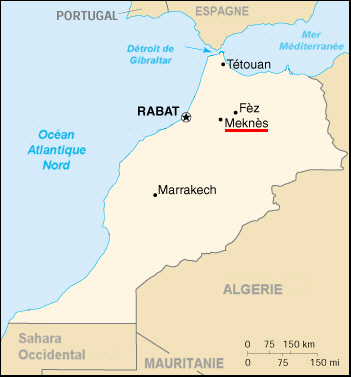
\includegraphics[width=0.66\textwidth]{maroc}
  \caption{Meknès, Maroc.}
  \label{fig:maroc}
\end{figure}

\section{Le \PaM}
%----------------------------------------------------------------------

Ce palais, aussi appelé \emph{Heri el-Mensour}, porte le nom de son 
constructeur, un chrétien converti à l'Islam. Il est situé au sud de 
la qasba (\fref{fig:meknes}). Bien que délabré aujourd'hui, cet 
édifice est encore impressionnant \autocite{Barrucand_1976}.

\begin{figure}[htb]
  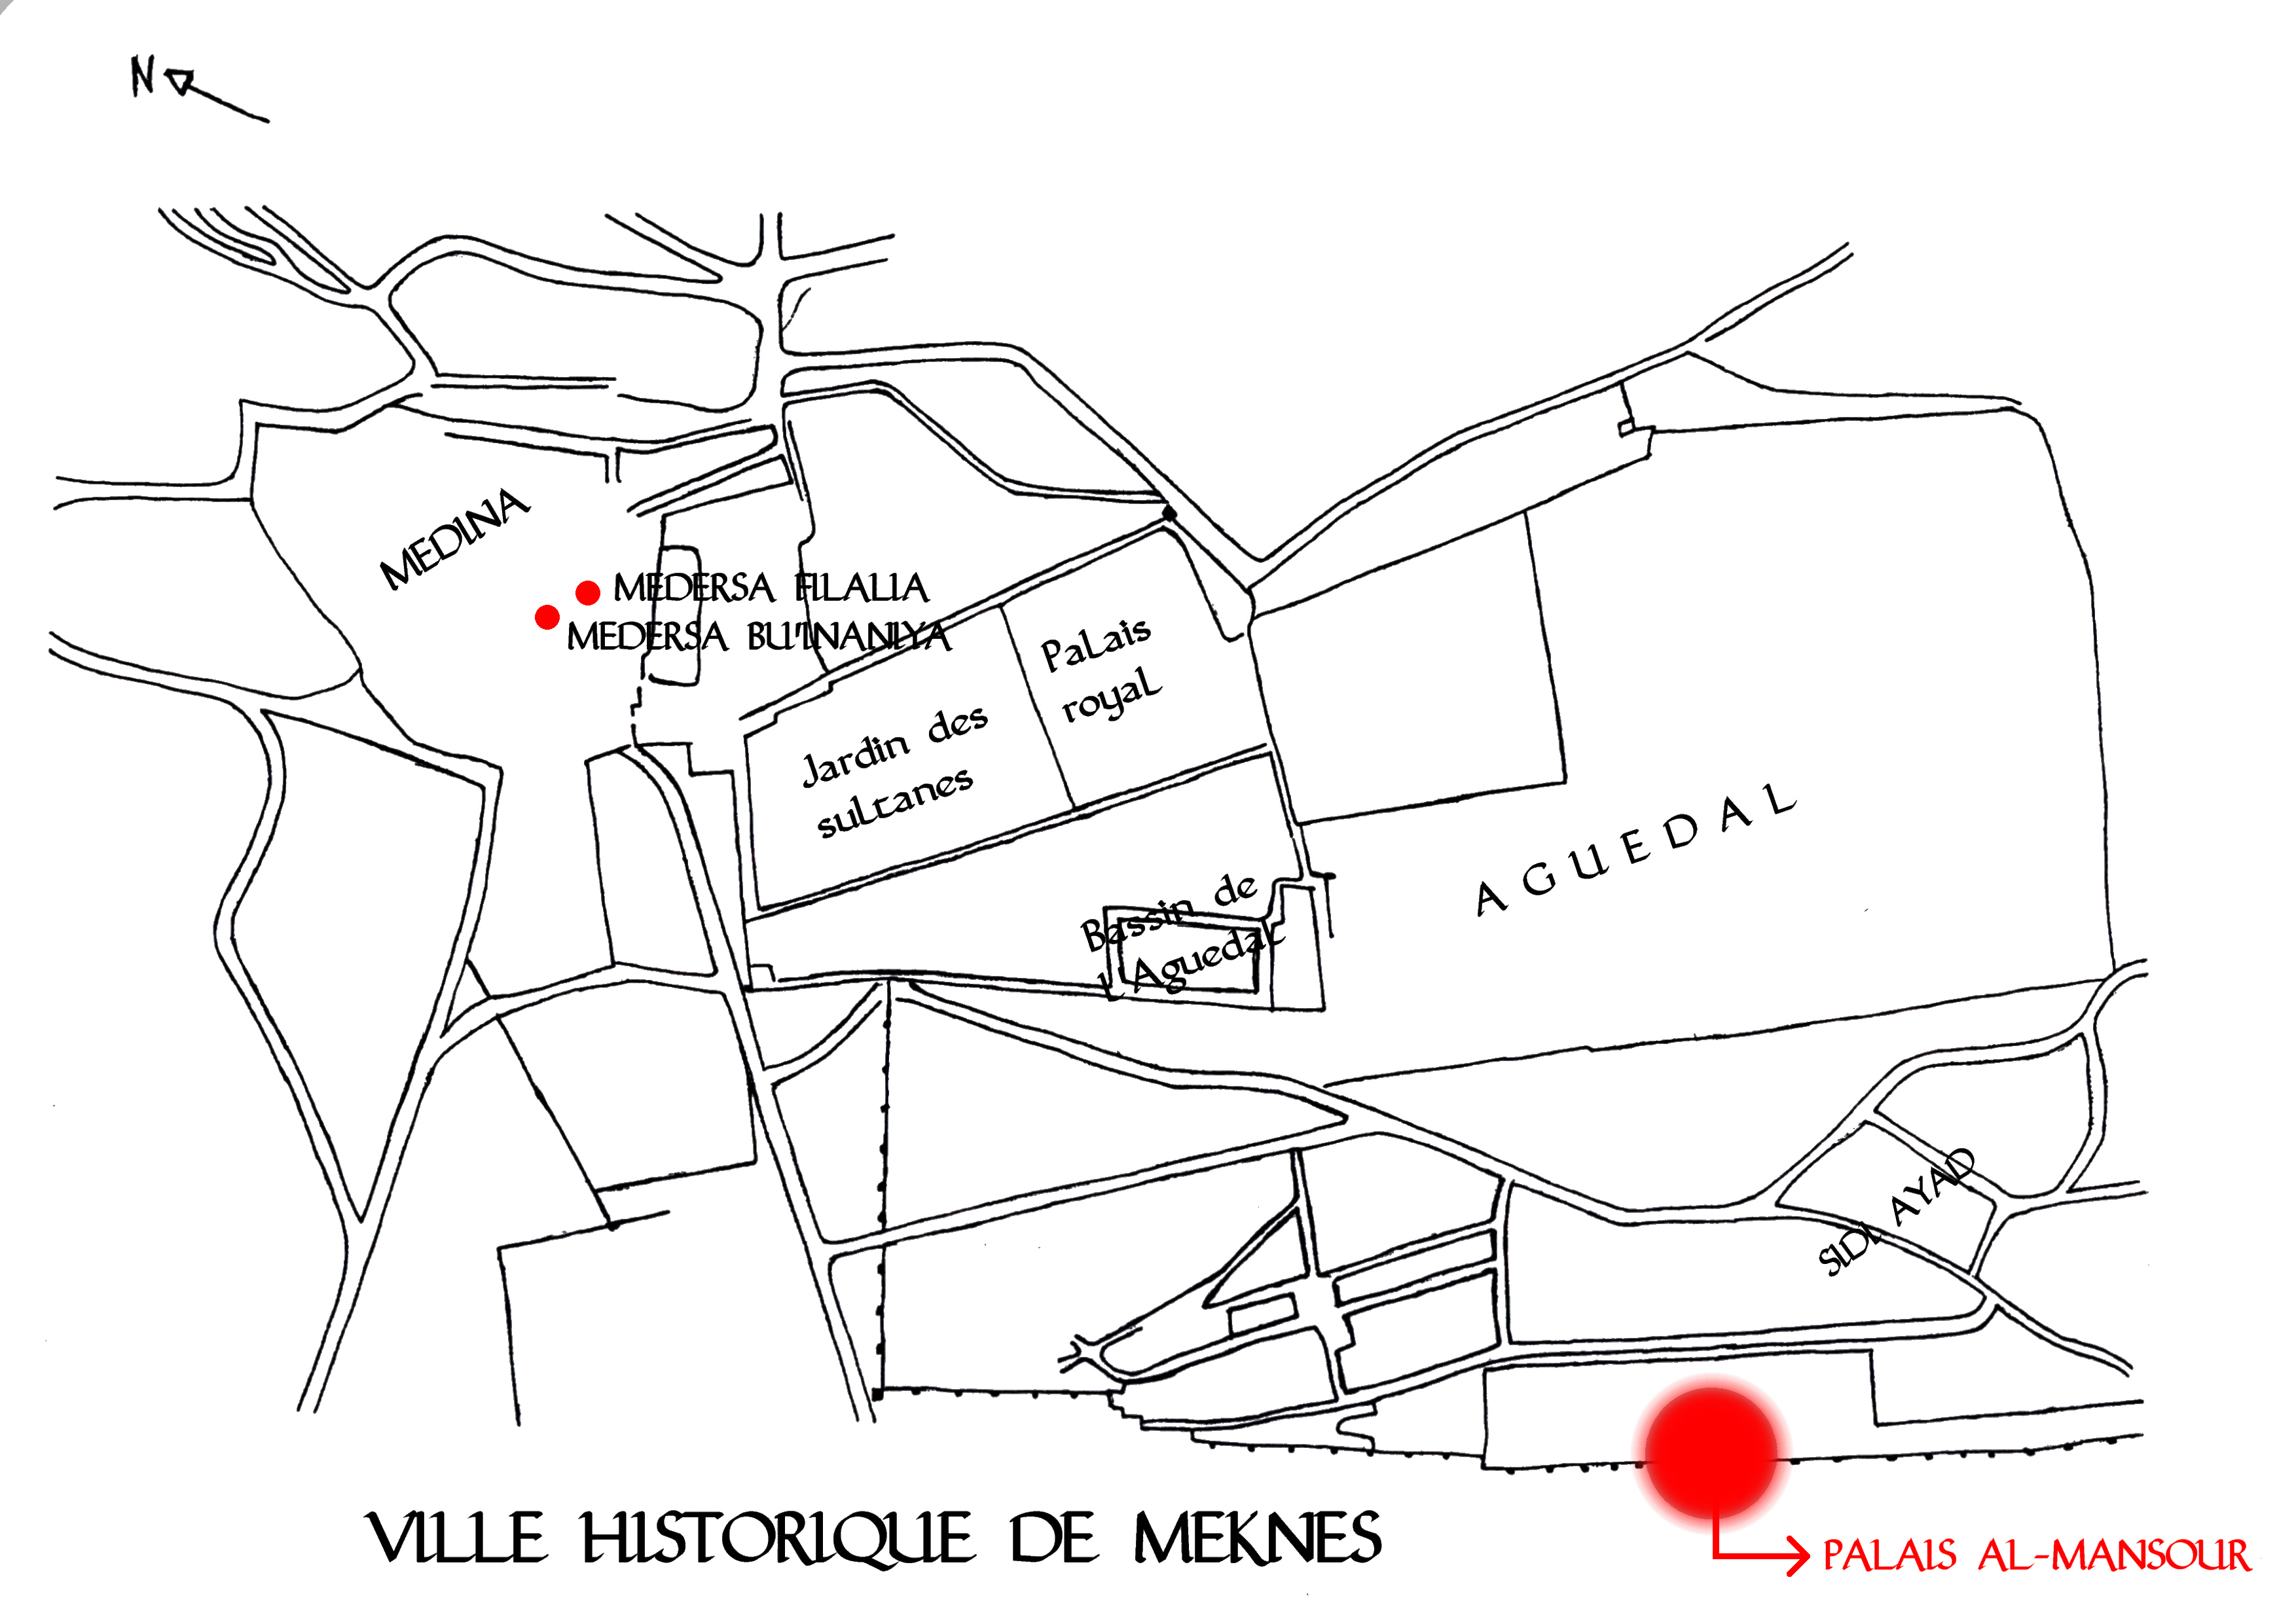
\includegraphics[width=0.95\textwidth]{meknes}
  \caption{Localisation du \PaM dans Meknès.}
  \label{fig:meknes}
\end{figure}

La première description du \PaM a été faite par Al-Zayyani : 
\frquote{Ismaïl avait encore fait construire dans la qasba un palais 
appelé al-Mansour : ce palais renfermait vingt coupoles, et chacune 
de ces coupoles avait une tour d'où l'on dominait le panorama formé 
par les plaines et les montagnes de Méquinez. {\dots} Il plafonne à 
plus de \num{100}~coudées : \num{50}~coudées pour le rez-de-chaussée 
et \num{50}~coudées pour le reste. Ce palais est composé de vingt 
salons, éclairés chacun par une fenêtre au milieu. Les fenêtres 
étaient grillagées et permettaient aux habitants d'avoir une vue des 
plaines de Meknès située toute entière entre deux montagnes. Les 
salons avaient un plafond en bois coloré et une toiture de tuiles 
vertes. Quatre de ces salons étaient longs de \num{70}~empans, les 
autres étant de \num{40}~empans de longs chacun {\dots}}
\autocite{Barrucand_1976}.

Il est surprenant de constater que ce bâtiment apparemment 
assez extraordinaire ne figure guère dans les récits des 
esclaves, ambassadeurs ou religieux qui ont décrit le Meknès du
\siecle{xvii}. Seul Joseph de Léon semble le connaître. Selon lui, 
les concubines tombées en disgrâce du sultan étaient reléguées dans ce 
palais périphérique. En fait, ce bâtiment aurait peut-être pu n'être 
construit qu'à l’extrême fin du règne de Moulay Ismaïl.

\begin{figure}[htb]
  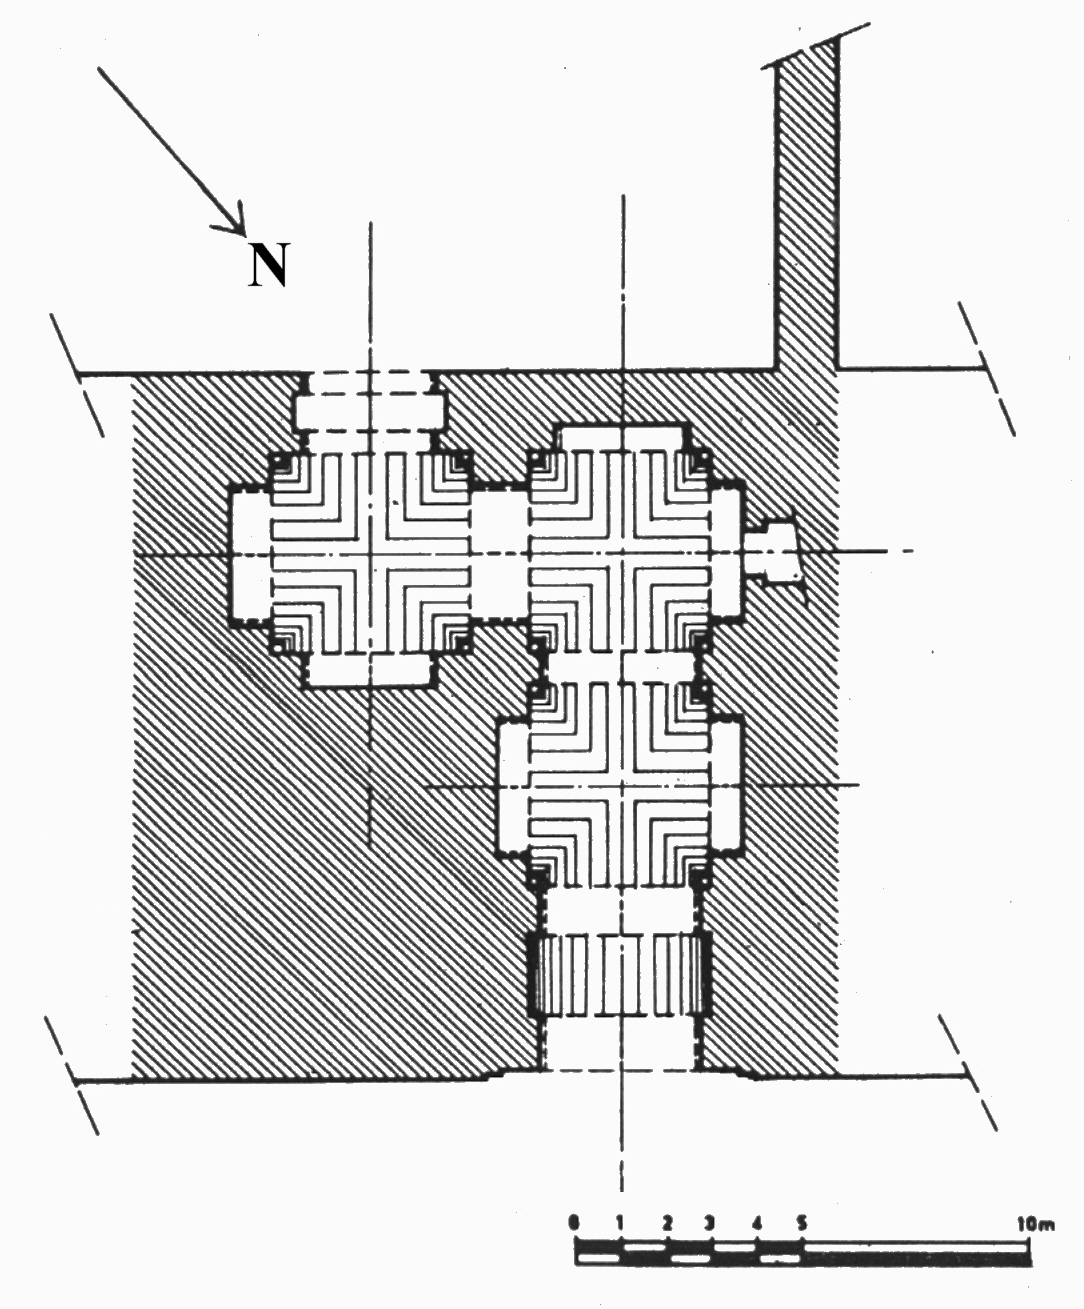
\includegraphics[width=0.66\textwidth]{palais}
  \caption{Palais al-Mansour, Meknès, \scl{xvii}. Plan d'ensemble 
           \autocite{Barrucand_1976}}
  \label{fig:palais}
\end{figure}

Le \emph{Heri el-Mensour} (\fref{fig:palais}) est une bâtisse de forme 
parallélépipédique dont la façade est longue de \SI{79}{\m} et dont la 
profondeur est de \SI{92}{\m}. Un bâtiment annexe qui abrite notamment 
\emph{Bab Heri el-Mensour} prolonge la façade de \SI{31}{\m} vers le 
sud-est.

La profondeur de cette construction mitoyenne est de \SI{12}{\m}. 
La hauteur du \emph{heri} varie entre 
\SIrange[range-phrase=\ et\ ]{12}{14}{\m} (\autocite{Barrucand_1976}.

Ce bâtiment comporte un rez-de-chaussée et un étage. Les témoignages 
littéraires et les constatations archéologiques ont permit de mettre 
en évidence les fonctions utilitaires et subalternes du 
rez-de-chaussée. L'étage supérieur (\fref{fig:etage}) semble avoir eu 
des fonctions nettement plus nobles. Il n'est accessible que par un 
escalier moderne remplaçant la rampe d'origine et situé dans l'angle 
nord-est de l'édifice. Il est dans un état de délabrement avancé. Les 
constructions se distribuent sur les deux longs côtés d'une grande 
cour centrale mesurant \SI{76.80}m sur \SI{25.45}{\m} Elles sont 
groupées dans une double rangée sur le côté sud et dans une triple 
rangée sur le côté nord \autocite{Barrucand_1976}.


\begin{figure}[htb]
  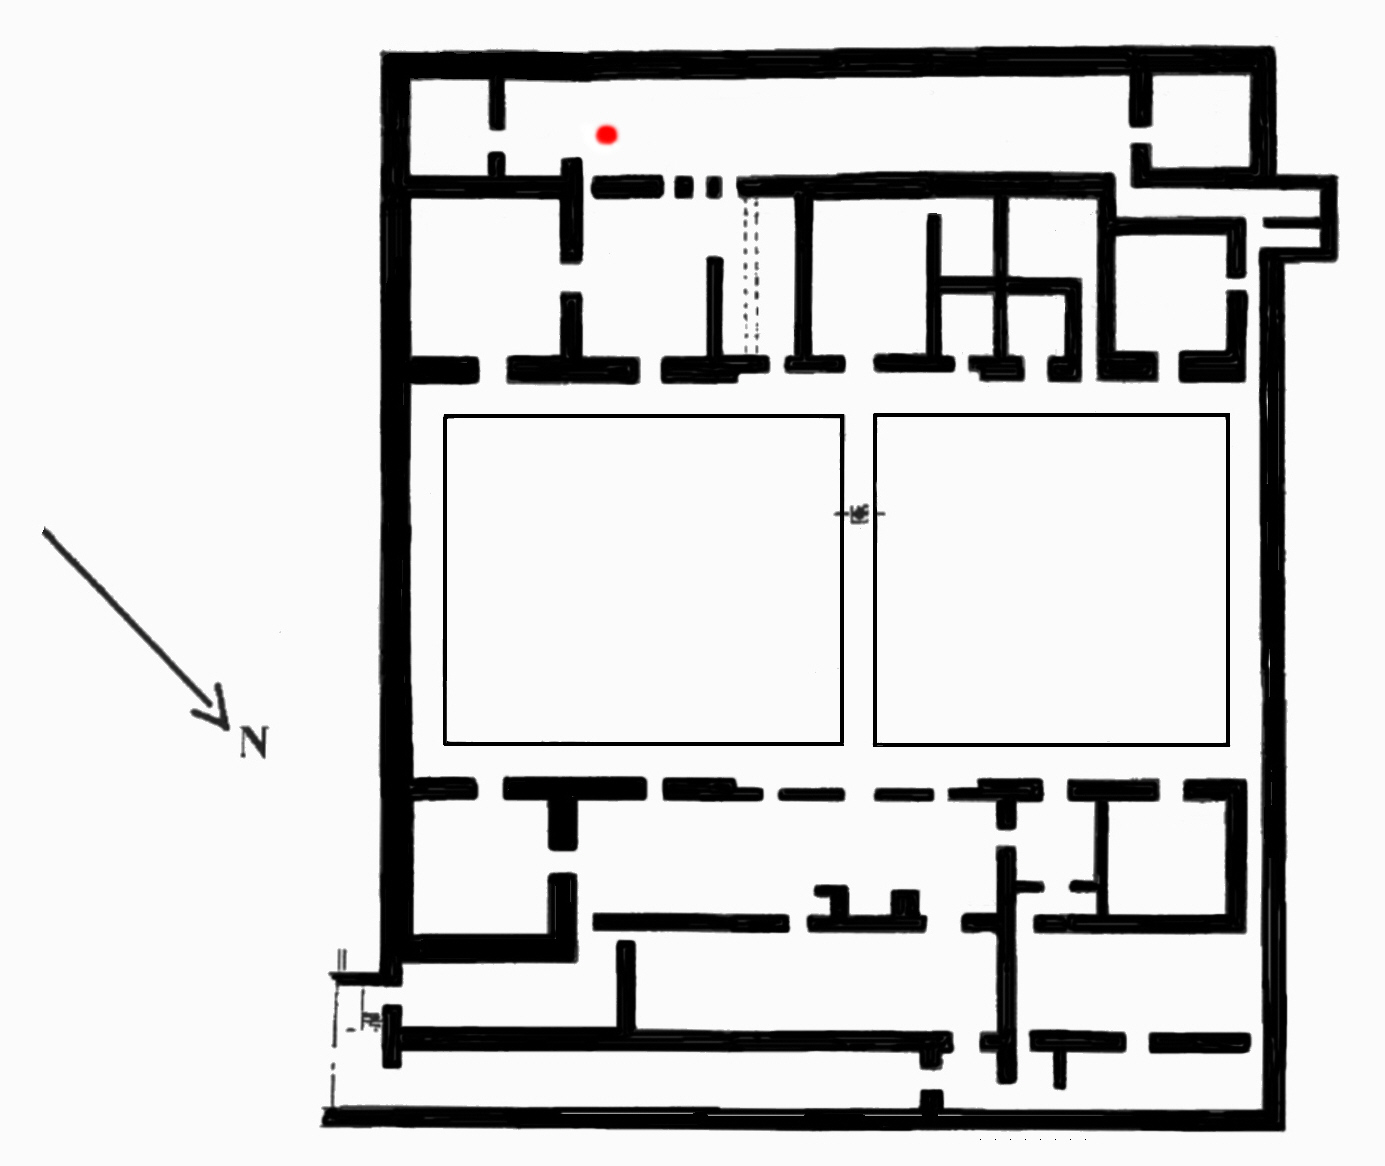
\includegraphics[width=0.8\textwidth]{palais_etage}
  \caption{Palais al-Mansour, Meknès, \scl{xvii}. 
           Plan de l'étage. En rouge : point de prélèvement 
           (réalisation : A.~\bsc{Benmlih} et M.~\bsc{Haddad})}
  \label{fig:etage}
\end{figure}

L'ordonnance de la cour étonne par son irrégularité. Il semble s'être 
agit d'une grande cour d'honneur mais il n'y a plus de restes d'un 
éventuel portique et les nombreuses ouvertures dans les flancs nord 
et sud, disposées sans aucun souci d'axialité, étaient surmontées 
indifféremment de linteaux plats ou d'arcs brisés outrepassés. On 
reconnaît certaines constructions à deux étages percées de fenêtres. 
Si cet étage avait réellement servi de palais à Moulay Ismaïl ou 
même seulement à ses concubines disgraciées, il aurait comporté 
\emph{hammams}, fours, et, bien entendu, salle de prière. 
Des investigations plus poussées seraient nécessaires pour cerner 
de plus près les destinations et l'aménagement de cet étage 
\autocite{Barrucand_1976}.

\section{Les échantillons}
%----------------------------------------------------------------------

Les cinq échantillons de zelliges (planche~1) ont été prélevés sur 
le sol d'une salle située à l'étage du \PaM, au sud de la grande cour 
centrale (\fref{fig:etage}). Ce sont des pièces de céramique glaçurée 
de forme parallélépipédique. Chacune comporte une glaçure monochrome. 
L'échantillon référencé \bdx{6528} présente une glaçure verte, le 
\bdx{6529}, une glaçure bleu-vert, le \bdx{6530}, une glaçure noire, 
le \bdx{6531}, une glaçure miel et le \bdx{6532}, une glaçure blanche. 
Il s'agit là des cinq couleurs de base de l'art des zelliges.

Le \bdx{6529} est sensiblement plus gros et plus épais que les autres 
et, contrairement à eux, n'est pas chanfreiné. Il s'agit probablement 
d'un carreau entourant les motifs de zelliges.


[Planche des échantillons]


\chapter{Méthodologie et expérimentation}
%======================================================================

\section{Mémorisation des échantillons}
%----------------------------------------------------------------------

La première étape, avant toute intervention sur l'échantillon, est sa 
mémorisation.

Dès son arrivée au laboratoire, l'échantillon est photographié, 
scanné, dessiné. On note également ses dimensions et sa masse.

Ces préliminaires sont indispensables pour conserver une image de 
l'objet dans son état initial.

Les prises de vue ont été réalisées à l'aide d'un boîtier 
photographique \num{24x36} muni d'un objectif macro Nikon. 
L'éclairage de l'objet est assuré par des lampes tungstène 
\SI{75}{\W}. Le film photographique utilisé a une sensibilité 
de \SI{64}{ASA}.

\section[SAO et \CHRO]
        {Étude de la couleur : \SAO et \CHRO}
%----------------------------------------------------------------------

\subsection[SAO]
           {Détermination des ions chromogènes : \SAO}
%~~~~~~~~~~~~~~~~~~~~~~~~~~~~~~~~~~~~~~~~~~~~~~~~~~~~~~~~~~~~~~~~~~~~~~
La couleur résulte de l'interaction entre lumière et matière. Dans le 
cas des verres silicatés, elle est due à l'absorption spécifique du 
rayonnement lumineux par des cations de métaux de transition ou des 
terres rares présents à l'état d'impuretés dans la structure du verre 
\autocite{Lajarte_1979}.

En \SAO en mode réflexion diffuse, l'échantillon est bombardé 
par un rayonnement électromagnétique monochromatique. La mesure du 
rayonnement réfléchi (détecteur : photomultiplicateur) par la surface 
analysée permet de déterminer le spectre d'absorption. Celui-ci peut 
présenter des bandes d'absorption caractéristiques des ions 
chromogènes responsables de la couleur.

L'appareillage utilisé est un spectrophotomètre UV-visible 
double-faisceau (CARY1, Varian). La gamme spectrale balayée s'étend 
de \SIrange[range-phrase=\ à\ ]{190}{900}{\nm}.
La source du rayonnement est une lampe tungstène dans l'infrarouge 
et le visible, une lampe au deutérium prend le relais à \SI{310}{\nm}. 
On utilise une cellule de polytétrafluoroéthylène (PTFE) pour calibrer 
le système et comme blanc de référence.

Pour effectuer des mesures sur des zones de faibles dimensions, 
nous avons utilisé un montage couplant un microscope optique au 
spectrophotomètre. L'objet à étudier est placé sur la platine du 
microscope, l'éclairage, de type halogène, est assuré par des fibres 
optiques Intralux~5000. La gamme spectrale balayée est alors comprise 
entre \SIrange[range-phrase=\ et\ ]{380}{750}{\nm}. La lumière 
réfléchie par l'échantillon et reçue par l'objectif du microscope est 
dirigée vers le détecteur du spectrophotomètre par l'intermédiaire 
d'une autre fibre optique. Une étude méthodologique a permis de 
montrer que les résultats obtenus par cette méthode ne diffèrent pas 
sensiblement de ceux obtenus avec le spectrophotomètre seul (Baras, 
2000, DESS).

Cette méthode est non-destructive et ne nécessite aucun prélèvement de 
matière. Les mesures sont effectuées directement sur l'échantillon.

Les spectres d'\AO présentés sont ceux de l'objet composite (glaçure + terre cuite). Ils n'ont pas été corrigés de la contribution du support céramique lorsque la glaçure est transparente.

\subsection[Chromamétrie]{Mesure physique de la couleur : \CHRO}
%~~~~~~~~~~~~~~~~~~~~~~~~~~~~~~~~~~~~~~~~~~~~~~~~~~~~~~~~~~~~~~~~~~~~~~
La définition d'une couleur est particulièrement subjective et dépend 
de la sensibilité spectrale de l'{\oe}il, de la nature de la lumière 
incidente, de l'état de surface de l'objet, mais aussi de la culture 
et de l'éducation de l'observateur (les papous, par exemple, n'ont pas 
de terme pour désigner le jaune (\textit{Pour la Science}, hors-série 
avril 2000)).

La \CHRO permet de définir les couleurs par leurs
coordonnées chromatiques. Elle repose sur le fait que toute couleur
peut être définie comme la superposition de trois couleurs dites
\frquote{primaires} : le rouge, le vert et le bleu.

Conformément aux conventions mises en place par la \emph{Commission 
Internationale de l'Éclairage}, les modes de représentations 
graphiques choisis correspondent aux systèmes \Yxy (CIE~1931) 
(\fref{fig:Yxy}) et \Lab (CIE~1976) (\fref{fig:Lab}).

Le système \Lab peut être déduit du système \Yxy par transformation 
non linéaire :

\begin{equation*}
  L^* = 116 \times \left(\frac{Y}{Y_n}\right)^{1/3} - 16
\end{equation*}

\begin{equation*}
  a^* = 500 \times \left\{%
      \left(\frac{X}{X_n}\right)^{1/3} - 
      \left(\frac{Y}{Y_n}\right)^{1/3}%
    \right\}
\end{equation*}

\begin{equation*}
  b^* = 200 \times \left\{%
      \left(\frac{Y}{Y_n}\right)^{1/3} - 
      \left(\frac{Z}{Z_n}\right)^{1/3}%
    \right\}
\end{equation*}

\noindent 
Avec $\frac{X}{X_n}$, $\frac{Y}{Y_n}$, $\frac{Z}{Z_n} > 0,008856$ \\
et $X_n$, $Y_n$, $Z_n$ : coordonnées du point de référence

Les paramètres $Y$ et $L^*$ représentent la réflectance, c'est à dire 
la fraction de l'intensité de lumière réfléchie par l'aire examinée. 
Les paramètres $x$ et $y$ indiquent respectivement la proportion de 
photons rouges et verts dans la lumière réfléchie. $z$, représentant 
la composante bleu, est relié à $x$ et $y$ par :

\begin{equation*}
  x + y + z = 1
\end{equation*}

$a^*$ représente la composante chromatique rouge-vert et $b*$ la 
composante bleu-jaune. L'espace \Lab, obtenu par transformation 
non linéaire de l'espace \Yxy, est particulièrement utilisé car 
c'est un espace uniforme : la distance de deux points de couleur 
est proportionnelle aux différences perçues par l'{\oe}il entre les 
réalisations colorées. Il est plus difficile de faire une corrélation 
entre écart chromatique et écart visuel dans le système \Yxy. 
En revanche, il permet l'obtention aisée de la longueur d'onde 
dominante $\lambda_d$ du rayonnement, c'est à dire la longueur d'onde 
de la radiation spectrale qui, mélangée à une quantité appropriée de 
lumière blanche donne une égalisation colorimétrique de la couleur 
donnée, et de la pureté d'excitation représentant la quantité de 
lumière saturée caractérisée par $\lambda_d$ dans le rayonnement.

\begin{figure}[htb]
  \begin{minipage}[b]{0.40\textwidth}%
    \centerfloat
    \begin{tikzpicture}
      \node [anchor=south west, inner sep=0] (image) at ( 0.00, 0.00) 
            {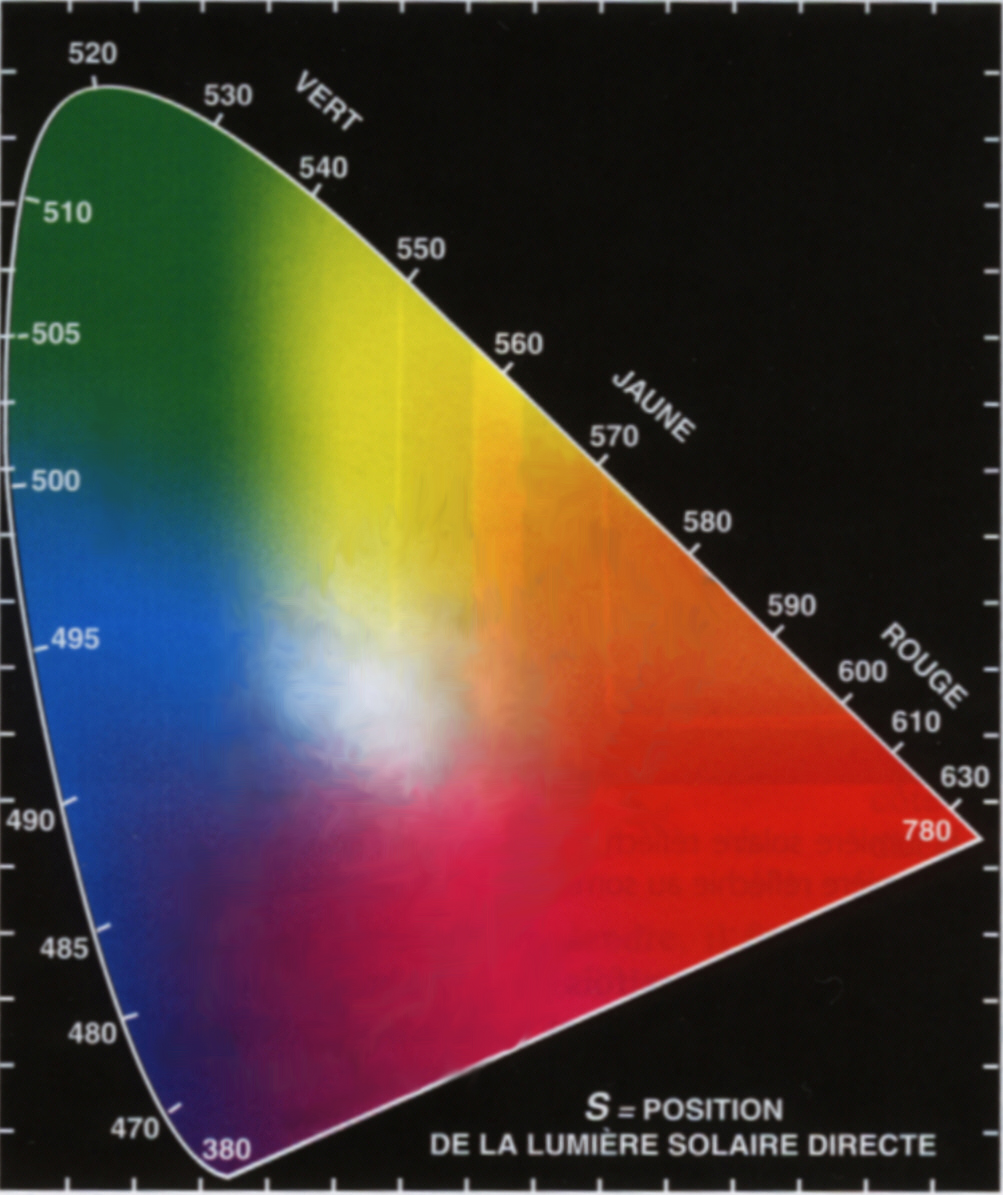
\includegraphics[width=\textwidth]{chroma_Yxy}} ;
      \begin{scope}[x={(image.south east)}, y={(image.north west)}]
        % \draw [step=0.05, help lines, white] (0, 0) grid (1, 1) ;

        \node [above] at ( 0.00, 1.00) {$\mathbf{y}$} ;
        \node [above right] at ( 1.00, 0.00) {$\mathbf{x}$} ;
      \end{scope}
    \end{tikzpicture}
    \subcaption{Système \Yxy (CIE~1931)\label{fig:Yxy}}
  \end{minipage}%
  \hfill%
  \begin{minipage}[b]{0.45\textwidth}%
    \centerfloat
    \begin{tikzpicture}
      \node [anchor=south west, inner sep=0] (image) at ( 0.00, 0.00) 
            {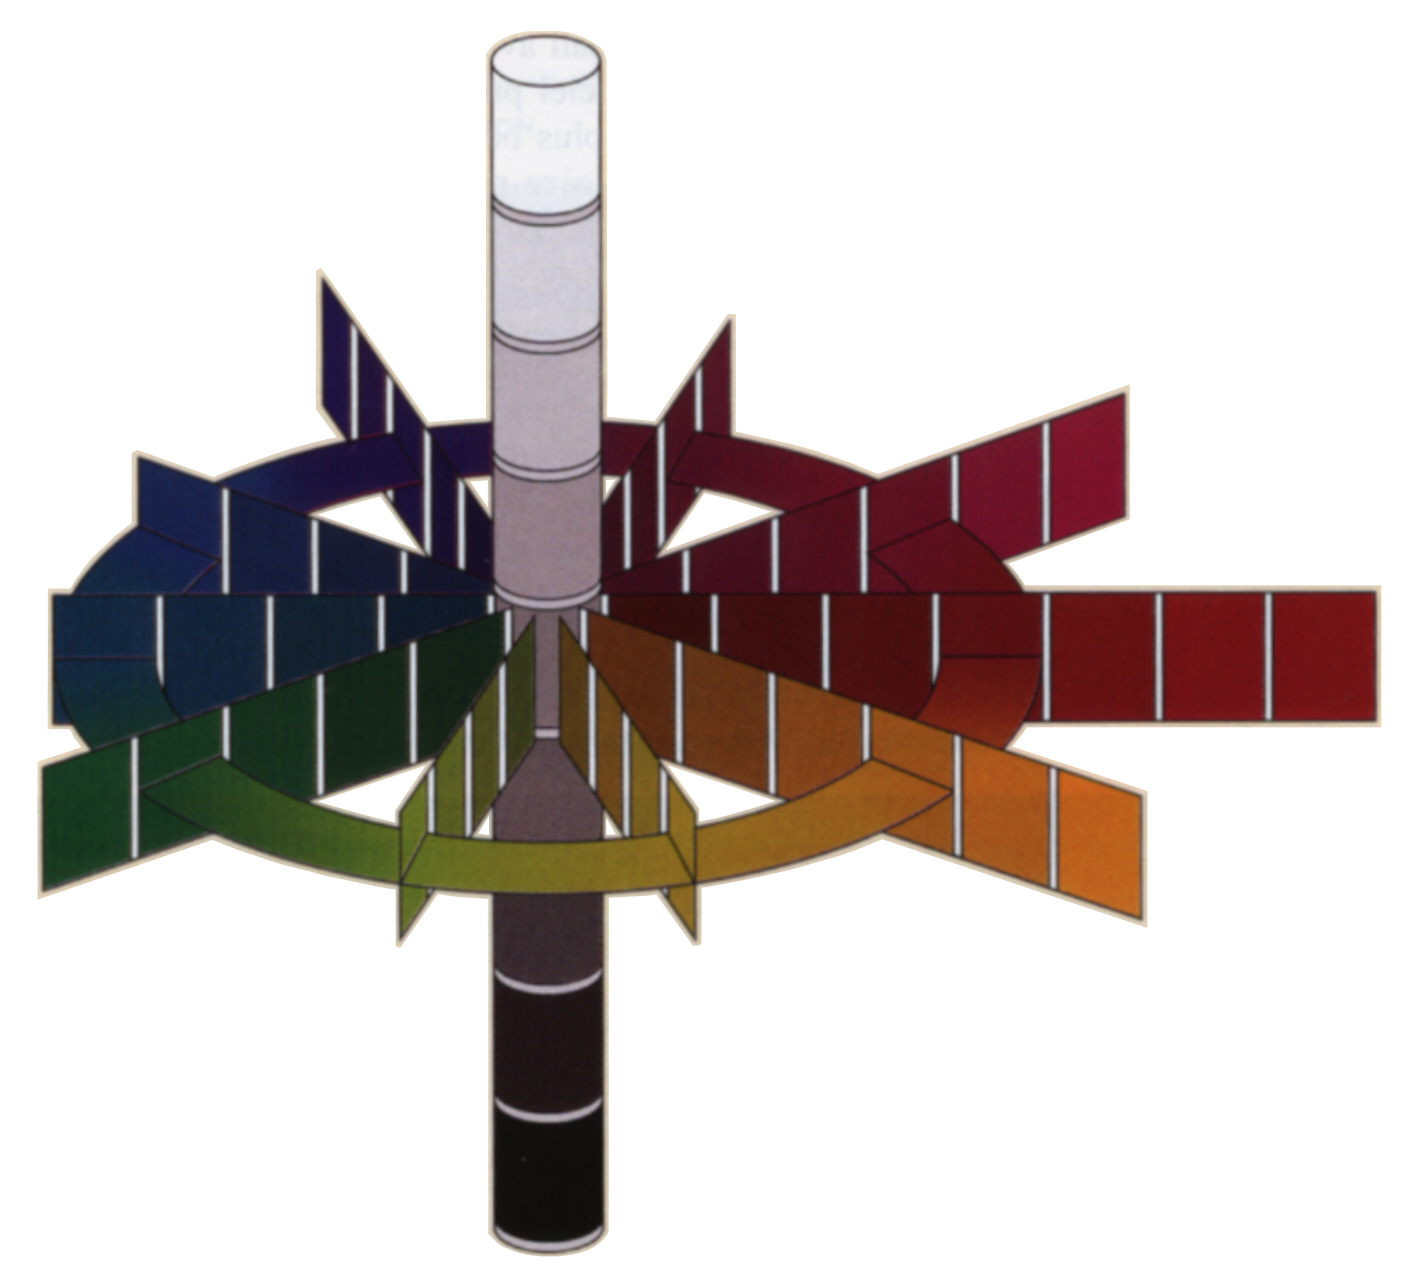
\includegraphics[width=\textwidth]{chroma_Lab}} ;
      \begin{scope}[x={(image.south east)}, y={(image.north west)}]
        % \draw [step=0.05, help lines, red] (0, 0) grid (1, 1) ;

        \node at ( 0.30, 0.90) {$\mathbf{L*}$} ;
        \node at ( 0.52, 0.25) {$\mathbf{b*}$} ;
        \node at ( 0.83, 0.67) {$\mathbf{a*}$} ;
      \end{scope}
    \end{tikzpicture}
    \subcaption{Système \Lab (CIE~1976)\label{fig:Lab}}
  \end{minipage}%
  \caption[Systèmes colorimétriques \trichro s]
          {Systèmes colorimétriques \trichro s (\emph{Pour la science}, hors série avril 2000)}
  \label{fig:colorimetrie}
\end{figure}

Les mesures colorimétriques sont réalisées à partir des spectres d'\AO, par l'intermédiaire du module \frquote{Chromamétrie} intégré dans le système d'exploitation des données du spectrophotomètre. Ces mesures sont effectuées par rapport à l'illuminant standard D65, avec un angle solide d'observation de \ang{2} et dans la plage de longueur d'onde \SIrange{400}{700}{\nm}.

\section{Étude de la texture}
%----------------------------------------------------------------------

\subsection{Observation en lumière naturelle}
%~~~~~~~~~~~~~~~~~~~~~~~~~~~~~~~~~~~~~~~~~~~~~~~~~~~~~~~~~~~~~~~~~~~~~~
Préliminaire indispensable à toute étude, l'observation macroscopique 
permet d'examiner l'état de surface d'un échantillon, la cohésion de 
l'ensemble glaçure/terre cuite, de localiser d'éventuels défauts ou 
anomalies liées à la cuisson ou au processus d'altération. Cette étape 
est indispensable pour repérer les zones qui feront ultérieurement 
l'objet d'analyses approfondies.

Cet examen peut s'effectuer sur l'échantillon brut sans prélèvement 
de matière ou sur une coupe perpendiculaire à la surface.

On utilise une loupe binoculaire à effet de zoom Olympus SZH. 
L'échantillon est éclairé par des fibres optiques Intralux~5000. 
Des prises de vue peuvent être faites grâce à un boîtier 
photographique Olympus~SC35.

\subsection{Observation en \CL}
%~~~~~~~~~~~~~~~~~~~~~~~~~~~~~~~~~~~~~~~~~~~~~~~~~~~~~~~~~~~~~~~~~~~~~~
La \CL est l'émission de lumière induite par bombardement électronique 
d'un matériau isolant ou semi-conducteur.

Ce phénomène est dû à la présence, dans le réseau cristallin de 
certains minéraux, de défauts ponctuels tels que des lacunes (d'ion 
négatif), des atomes interstitiels ou de substitution (terres rares 
ou métaux de transition essentiellement), faisant apparaître des 
niveaux donneurs ou accepteurs d'électrons dans la bande interdite. 
Sous l'effet d'une excitation extérieure (ici un flux électronique), 
ces défauts peuvent capturer des électrons ou des trous. Leur 
désexcitation s'effectue par émission de photon dans le domaine 
du visible (\fref{fig:CL_principe}). On appelle ces défauts des 
\emph{centres luminogènes} ou \emph{centres colorés}.

La couleur de la luminescence dépend donc de défauts souvent caractéristiques d'un minéral et permet ainsi, avec l'appui de la \DX, l'identification des phases cristallines présentes dans un matériau (Bechtel, Platel, 2000).

L'observation en \CL donne également une idée de l'homogénéité de 
l'échantillon.

L'appareillage de \CL (\fref{fig:CL_app}) est constitué d'une chambre 
de type NUCLIDE maintenue sous vide primaire (\SI{5e-2}{\milli\bar}), 
d'un canon à électrons (cathode froide d'acier). La tension 
d'accélération est de l'ordre de \SI{10}{\kV} et l'intensité du 
courant se situe entre \SIrange[range-phrase=\ et\ ]{0.85}{0.95}{\mA}. 
Ce système est couplé à une loupe binoculaire et à une caméra 3CCD 
(Sony~DXC-930\,P) permettant l'enregistrement photographique.

\begin{figure}[htb]
  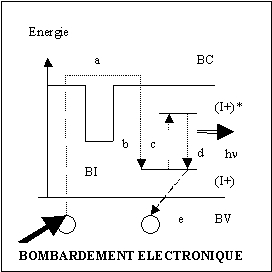
\includegraphics[width=0.5\textwidth]{CL_principe}
  \caption[Principe de la \CL]{Principe de la \CL. 
a : ionisation d'un atome sans intervention d'un centre piège ;
b : capture de l'électron par l'impureté \ce{(I+)} ;
c : excitation en \ce{(I+)*} ;
d : désexcitation radiative ;
e : recapture de l'électron dans la bande de valence (il n'y a pas 
forcément ionisation, l'électron peut directement être capturé par 
l'impureté) ;
BV : bande de valence ;
BC : bande de conduction ;
BI : bande interdite.
\autocite{web_CL}}
  \label{fig:CL_principe}
\end{figure}
% (\url{http://loic.portelette.free.fr/aasaann.html}, avril 2000)

\begin{figure}
  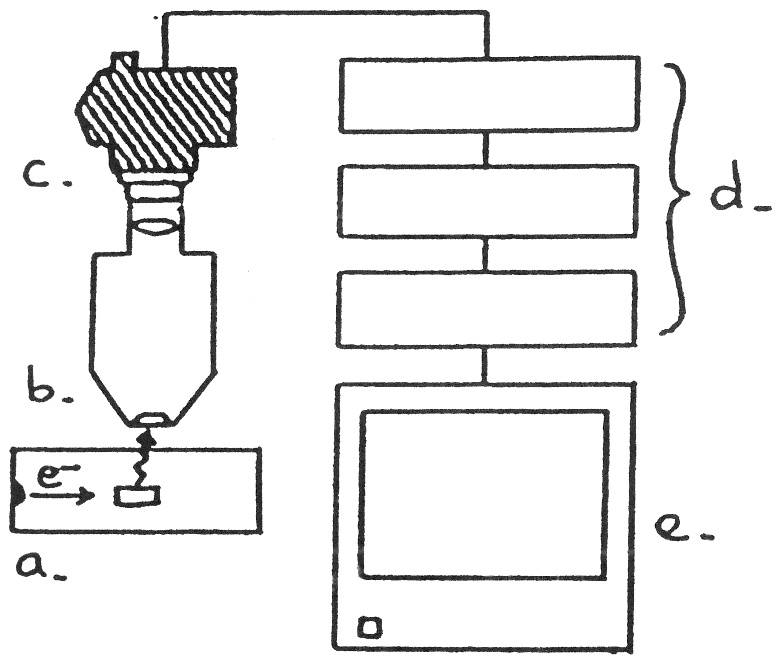
\includegraphics[width=0.5\textwidth]{CL_app}
  \caption{Appareillage de \CL.
           a : chambre Nuclide ;
           b : loupe binoculaire ;
           c : caméra~3CCD ;
           d : système d'acquisition et de traitement ;
           e : moniteur.}
  \label{fig:CL_app}
\end{figure}

L'analyse est généralement effectuée sur une lame, épaisse ou mince, 
taillée perpendiculairement à la surface glaçurée de l'échantillon et 
polie pour présenter la surface la plus plane possible.

Les lames sont réalisées à partir de prélèvement inclus dans une 
résine araldite. La découpe se fait à l'aide d'une scie à fil 
diamanté. On utilise pour le polissage des poudres de carbure 
de silicium (\SIrange[range-phrase=\ et\ ]{37}{9}{\um}) et des
suspensions diamantées de granulométrie progressive 
(\SIlist{6;3;1;0.1}{\um}).

\subsection{Observation en \MEB[ie]}
%~~~~~~~~~~~~~~~~~~~~~~~~~~~~~~~~~~~~~~~~~~~~~~~~~~~~~~~~~~~~~~~~~~~~~~
Le \MEB (MEB) est un instrument de visualisation permettant 
l'identification et la caractérisation de matériaux homogènes 
ou hétérogènes sur des surfaces allant du \si{\mm\squared} au
\si{\nm\squared} (grossissements de \texttimes\num{10} à 
\texttimes\num{300000}).

Il existe trois modes de formation des images en \MEB[ie] résultant 
de trois types d'interactions électrons-matière :

\begin{itemize}
  \item \uline{Imagerie en mode \emph{électrons secondaires}}\\
        Le faisceau peut provoquer l'arrachement d'électrons 
        périphériques des atomes de l'échantillon, ce sont les 
        électrons secondaires (\fref{fig:meb}). De faible énergie 
        (E=\SI{200}{\electronvolt}), ils proviennent de la surface 
        de l'échantillon et donnent une image de sa topographie. 
  \item \uline{Imagerie en mode \emph{\ERD}}\\ 
        Les \ERD (\fref{fig:meb}) proviennent de la diffusion 
        élastique ou quasi-élastique du faisceau incident. Ils ont 
        donc une énergie élevée, voisine de l'énergie incidente. 
        Les images obtenues présentent un contraste de composition : 
        en effet, le coefficient de rétrodiffusion est fonction de 
        la densité électronique, et donc du numéro atomique. 
        Autrement dit, les zones de l'échantillon correspondant aux 
        éléments les plus lourds, apparaîtront à l'écran plus claires, 
        plus \frquote{brillantes}. Les éléments légers correspondront 
        aux zones les plus noires de l'image.
  \item \uline{Imagerie par émission de \RX : \emph{\carto~X}}\\
        Le bombardement électronique primaire provoque aussi 
        l'émission de \RX caractéristiques de l'élément émetteur 
        (\fref{fig:meb}). Les cartes ainsi obtenues fournissent des 
        informations qualitatives sur la répartition des éléments 
        présents dans une couche superficielle.
\end{itemize}

\begin{figure}[htb]
  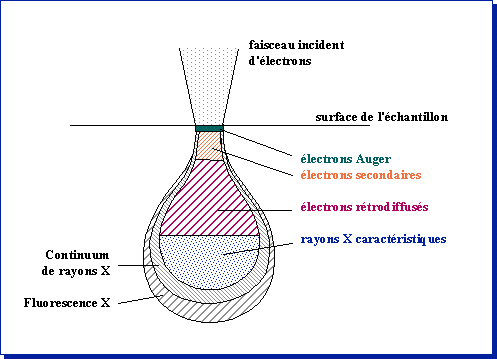
\includegraphics[width=0.6\textwidth]{meb}
  \caption[Poire d'interaction électrons-matière]
          {Poire d'interaction électrons-matière \autocite{web_MEB}}
  \label{fig:meb}
\end{figure}
% (\url{http://www.culture.fr/culture/conservation/fr/méthodes/méthodes.htm}, juin 2000)

\section{Détermination des compositions élémentaires : \spectro de 
         \RX en dispersion d'énergie}
%----------------------------------------------------------------------

Pour déterminer les compositions élémentaires (majeurs et mineurs), 
on utilise l'analyse quantitative par \EDS (EDS).

L'échantillon à analyser est irradié par des électrons. L'interaction 
électrons-matière se traduit par différents phénomènes parmi lesquels 
l'émission de \RX. On obtient ainsi un spectre de raies se détachant 
du fond continu (rayonnement de freinage ou \emph{Bremsstrahlung}) 
caractéristique des éléments constitutifs de la matière. La méthode 
consiste à comparer l'intensité $I_A$ (en nombre de coups) 
correspondant à un élément $A$ de l'échantillon à celle produite 
dans les mêmes conditions par un échantillon témoin contenant $A$ 
en concentration connue. On a la relation suivante :

\begin{equation*}
  \frac{C_\text{A}}{C_\text{A témoin}} = 
                      k \frac{I_\text{A}}{I_\text{A témoin}}
\end{equation*}


avec%
\begin{description}
  \item [$C_\text{A}$] concentration en~A de l'échantillon
  \item [$C_\text{A témoin}$] concentration en~A du témoin
  \item [$I_\text{A}$] intensité du rayonnement correspondant à~A pour 
        l'échantillon
  \item [$I_\text{A témoin}$] intensité du rayonnement correspondant 
        à~A pour le témoin
  \item [$k$] facteur de correction ZAF
\end{description}

$k$ est un facteur correctif qui tient compte des différences de 
composition entre l'échantillon à analyser et le témoin. Il exprime 
les effets de matrice (on appelle matrice l'ensemble des éléments de 
l'échantillon en dehors de l'élément à analyser) tels que :

\begin{itemize}
  \item \uline{Effet de numéro atomique} : Pour une valeur incidente 
        égale, l'intensité électronique arrivant en un atome~A est 
        différente dans l'échantillon et dans le témoin, car les 
        électrons subissent des effets différents avant d'arriver en~A.
        La diminution d'intensité et d'énergie du faisceau dépend du 
        numéro atomique des éléments constituants ; il est nécessaire 
        d'en tenir compte par une correction dite \emph{correction de 
        numéro atomique} exprimée par le facteur~$k_\text{Z}$.
  \item \uline{Effet d'absorption} : L'absorption du rayonnement~X 
        caractéristique sur son trajet de sortie dépend également 
        de la composition. Le rapport des intensités après absorption
        dans l'échantillon et dans le témoin est différent du rapport 
        des intensités primaires émises ; on en tient compte par 
        la \emph{correction d'absorption} exprimée par le
        facteur~$k_\text{A}$.
  \item \uline{Effet de fluorescence} : Le rayonnement caractéristique 
        à mesurer peut également être produit par émission~X de 
        fluorescence, sous l'action de rayonnements~X caractéristiques 
        émis par des atomes B de la matrice plus lourds que les atomes 
        A. L'intensité mesurée est la somme des intensités primaire et 
        secondaire sortantes, après absorption. L'effet de 
        fluorescence étant différent dans l'échantillon et dans le 
        témoin, il faut en tenir compte par la \emph{correction de 
        fluorescence} exprimée par le facteur~$k_\text{F}$.
\end{itemize}

Au total, on a : $k = k_\text{Z} + k_\text{A} + k_\text{F}$

Le facteur k, nécessaire au calcul des concentrations, est calculé par 
une méthode itérative, dite \frquote{méthode ZAF}, avec, comme point 
de départ, $k=1$.

Pour que les comparaisons entre les intensités relatives à 
l'échantillon et celles relatives au témoin soient valables, les 
mesures doivent être effectuées dans les mêmes conditions de géométrie 
d'émission (même distance de travail, notamment) et de courant de 
sonde. Or, ce dernier est très variable. Pour remédier à ce dernier 
problème, on procède à une calibration par rapport à la raie $K_a$ 
du cobalt, dont le spectre a été enregistré en même temps que les 
spectres des témoins, et le système procède à des corrections pour 
se ramener aux conditions correspondant aux témoins.

On peut analyser les éléments à partir de $Z=5$ (bore), 
la résolution énergétique est de 
\SIrange[range-phrase=\ à\ ]{130}{150}{\electronvolt}, la limite de 
détection est de l'ordre de \SI{1000}{ppm}.

Les analyses quantitatives présentées dans ce mémoire sont données 
en pourcentages massiques d'oxyde normalisés à \SI{100}{\percent}. 
Ce sont des moyennes de trois à cinq mesures effectuées sur toute la 
longueur de la glaçure ou de la terre cuite, sur la zone d'analyse 
la plus grande possible, et en prenant garde d'éviter les bulles et 
cristaux non fondus. Ceci dans l'hypothèse où la \CL a permis de 
montrer l'homogénéité du matériau. L'oxygène est quantifié par 
différence.

On utilise un spectromètre de \RX en dispersion d'énergie couplé au 
\MEB (JEOL~850SM) et muni d'un détecteur semi-conducteur \ce{Si(Li)}.

\section[Diffraction de \RX]{Détermination des compositions \cristallo s : \DX sur poudre}
%----------------------------------------------------------------------

L'état cristallin est caractérisé par une structure ordonnée et tripériodique. L'analyse par \DX sur poudre permet l'identification des phases cristallisées présentes dans un échantillon polycristallin.

Les \RX ont une longueur d'onde de l'ordre de la distance 
interatomique. Ils peuvent donc être diffractés par les plans 
interréticulaires du cristal selon la loi de Bragg :


\begin{equation*}
  n \lambda = 2 d \cdot sin\theta
\end{equation*}

\bigskip

\begin{minipage}{0.45\textwidth}
  \begin{description}
    \item [$d$] distance interréticulaire
    \item [$\lambda$] longueur d'onde des \RX incidents
    \item [$\theta$] angle d'incidence des \RX par rapport à la 
          famille de plans réticulaires
    \item [$n$] ordre de diffraction
  \end{description}
\end{minipage}%
\hfill%
\begin{minipage}{0.45\textwidth}
  \begin{tikzpicture}[x=10mm, y=7mm]
    \draw (-3.00, 0.00) -- ( 3.00, 0.00) ;
    \draw (-3.00, 1.00) -- ( 3.00, 1.00) ;
    \draw (-3.00,-1.00) -- ( 3.00,-1.00) ;

    \begin{scope}[red, thick, >=Straight Barb]
      \begin{scope}[postaction={decorate}, decoration={markings, 
                    mark=at position 0.75 with 
                    {\arrow[scale=1.67]{>};}}]
        \draw [postaction={decorate}] ( 0.00, 0.00) -- ++ (  40:3) ;
        \draw [postaction={decorate}] ( 0.00, 1.00) -- ++ (  40:3) ;
      \end{scope}
      \begin{scope}[postaction={decorate}, decoration={markings, 
                    mark=at position 0.75 with 
                    {\arrowreversed[scale=1.67]{>};}}]
        \draw [postaction={decorate}] ( 0.00, 0.00) -- ++ ( 140:3) ;
        \draw [postaction={decorate}] ( 0.00, 1.00) -- ++ ( 140:3) ;
      \end{scope}
    \end{scope}

    \begin{scope}[shift={(3.25, 0.00)}]
      \draw [<->] ( 0.00, 0.00) -- ( 0.00, 1.00) 
            node [midway, right] {$d$} ;
    \end{scope}

    \draw ( 1.00, 0.00) arc (0:40:1) ;
    \draw (-1.00, 0.00) arc (180:140:1) 
          node [midway, left] {$\theta$} ;
    \draw ( 1.00, 1.00) arc (0:40:1) ;
    \draw (-1.00, 1.00) arc (180:140:1) ;
  \end{tikzpicture}
\end{minipage}

\bigskip

Dans la méthode de \DX sur poudre, le matériau à analyser est bombardé par un faisceau de \RX monochromatiques et parallèles, de longueur d'onde connue. L'échantillon, de quelques milligrammes, est étalé sous forme de poudre sur une lame de verre animée d'un mouvement de rotation uniforme autour d'un axe situé dans son plan (cercle goniométrique). De cette manière, chaque famille de plans réticulaires se présente sous toutes les orientations possibles par rapport au faisceau~X incident. Un détecteur mesure l'intensité du rayonnement~X diffracté. Il tourne autour du même axe que l'échantillon mais avec une vitesse double.

Le diffractogramme obtenu présente des raies, caractéristiques des 
phases cristallines présentes. L'identification s'effectue à l'aide 
d'un logiciel basé sur les fiches de référence ASTM (\emph{American 
Society for Testing and Materials}). La limite de détection est de 
\SI{2}{\percent}.

\begin{figure}[htb]
  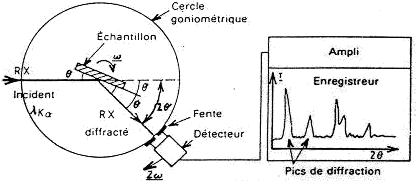
\includegraphics[width=0.6\textwidth]{DX}
  \caption{Appareillage de \DX}
  \label{fig:DX}
\end{figure}

L'équipement utilisé au laboratoire est un diffractomètre de 
poudre (\fref{fig:DX}) SIEMENS~D500. La source de \RX est une 
anticathode de cuivre ($\lambda=\SI{1.54}{\angstrom}$, 
$V=\SI{40}{\kV}$, $I=\SI{30}{\mA}$). Le domaine angulaire choisi 
pour l'étude s'étend de \ang{5} à \ang{60}.


\part{Résultats expérimentaux}
%!TEX root = MemoireZelliges.tex

\chapter{Étude physique d'un zellige vert (\bdx{6528})}
%======================================================================

\section{Description -- État de surface}
%----------------------------------------------------------------------

Cet échantillon, de forme parallélépipédique, est une pièce de 
céramique glaçurée de couleur verte (\fref{dessin:6528}). 
Il provient du \PaM (\siecle{17}) de Meknès. 
Il est chamfreiné. Les taches violacées sur la glaçure sont des 
traces d'encre dues à l'indexation de l'échantillon par les marocains.

\begin{itemize}
  \item \DimText : \SI{33x33x18}{\mm}
  \item \emph{Masse} : \SI{25.0}{\g}
\end{itemize}

\begin{figure}[htb]
  \begin{minipage}[t]{6.3cm}
    \centerfloat
    \vspace*{0pt}
    % Dessin de l'échantillon : Vue de dessus
    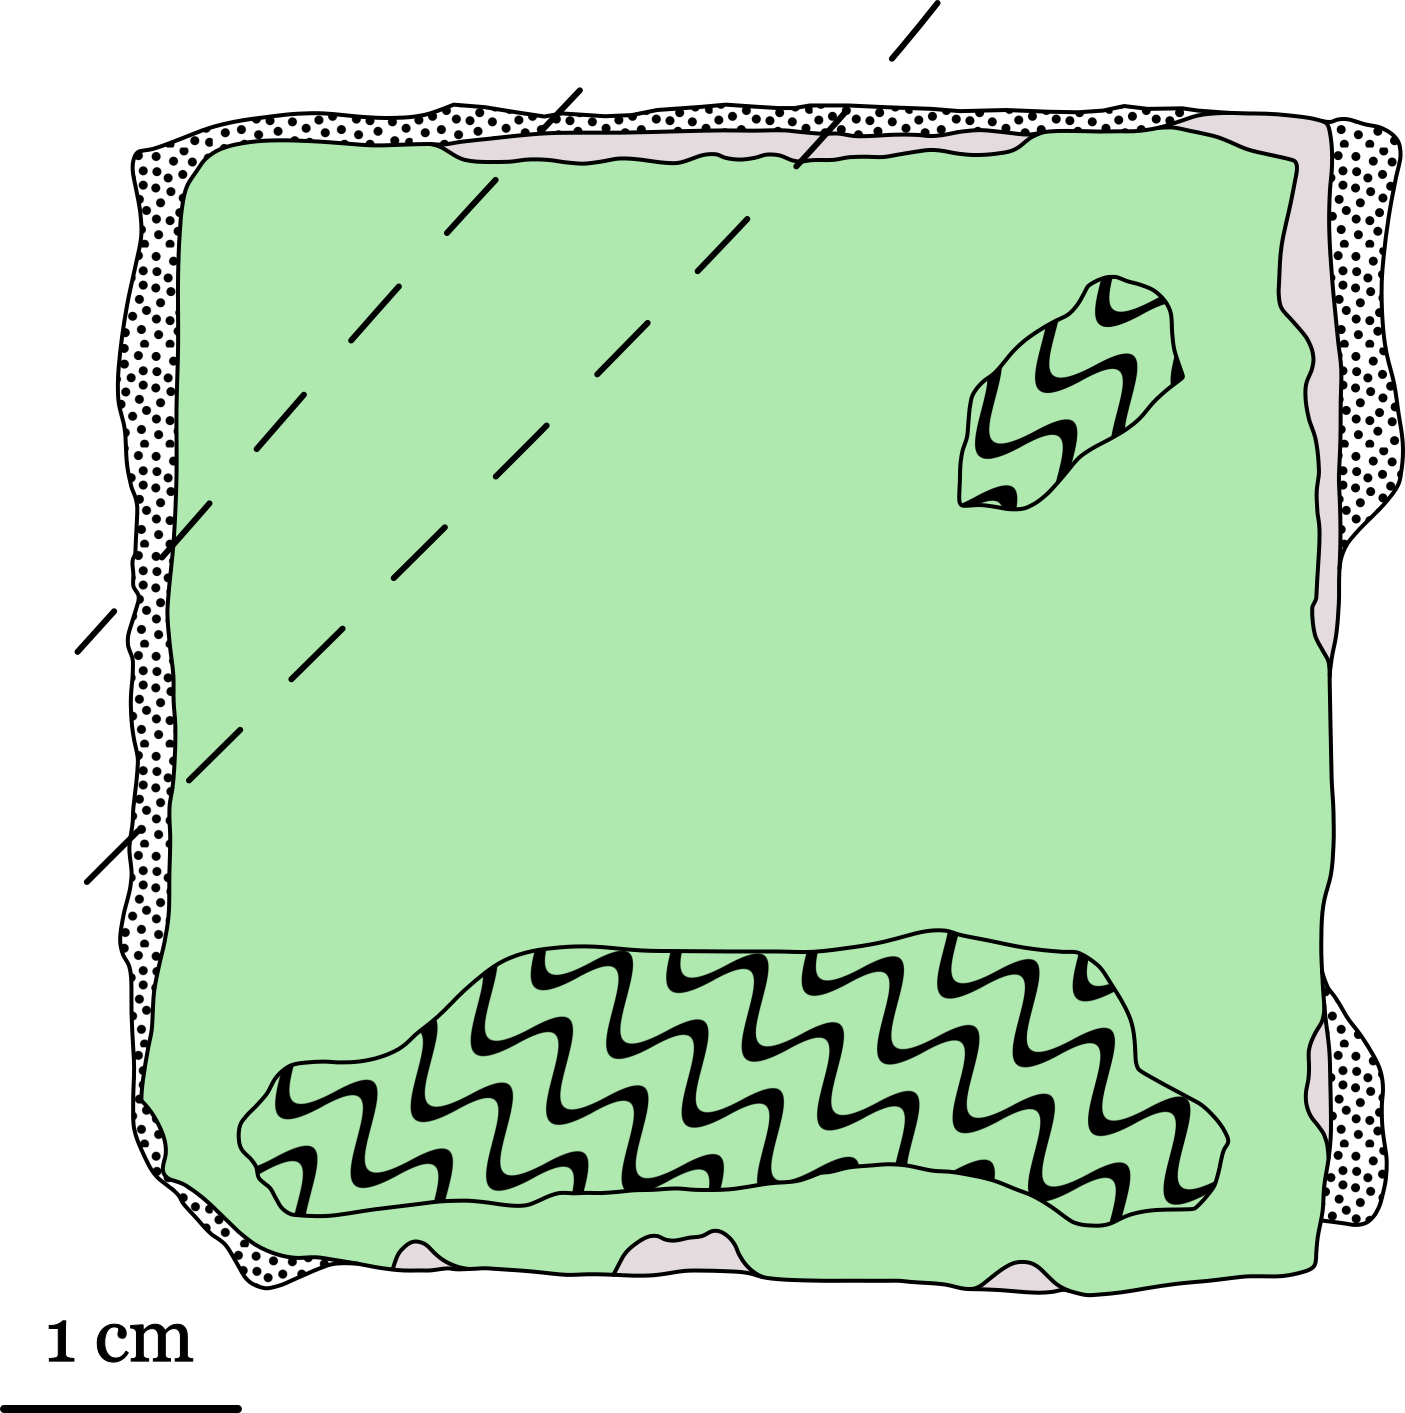
\includegraphics[scale=0.17]{PaM_BDX6528_dessus}
    \subcaption{Vue de dessus \label{dessin:6528_dessus}}

    \bigskip
    \bigskip
    \bigskip

    % Dessin de l'échantillon : Coupe
    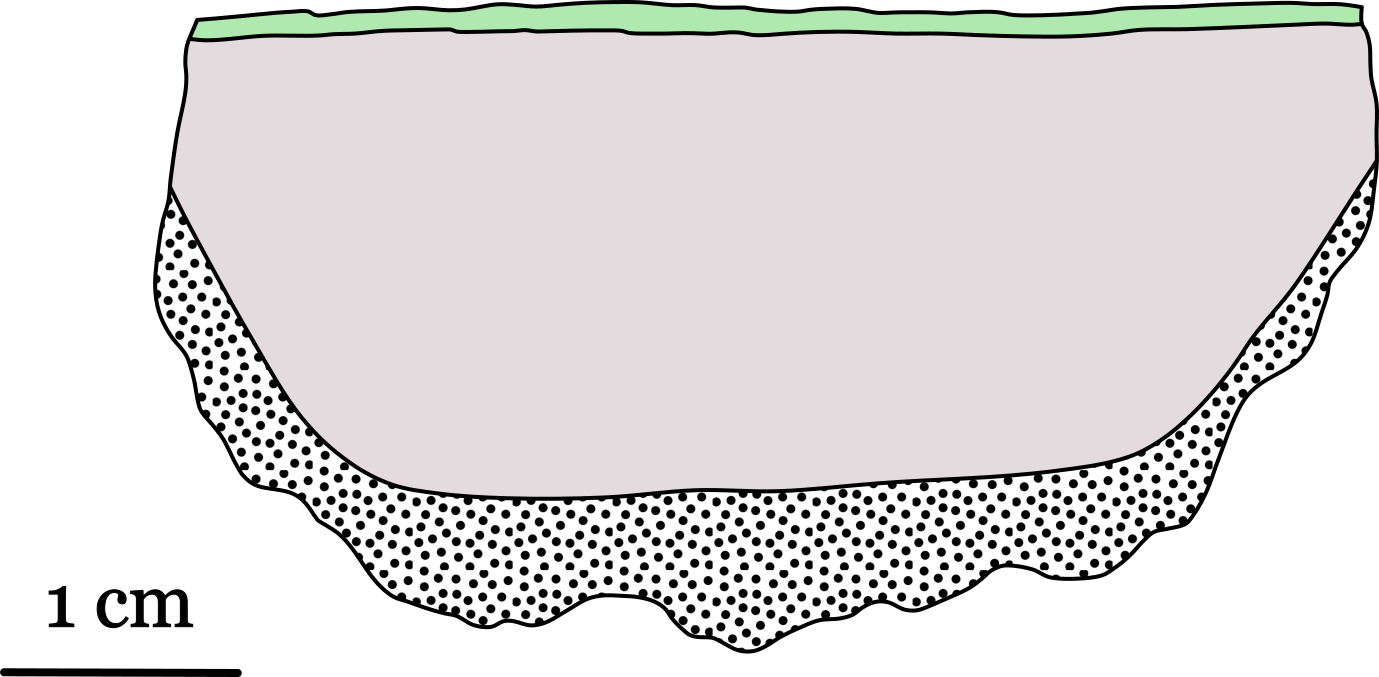
\includegraphics[scale=0.17]{PaM_BDX6528_coupe}
    \subcaption{Vue en coupe \label{dessin:6528_coupe}}
  \end{minipage}%
  \qquad%
  \begin{minipage}[t]{6.2cm}
    \centerfloat
    \vspace*{0pt}
    % Dessin de l'échantillon : Lame
    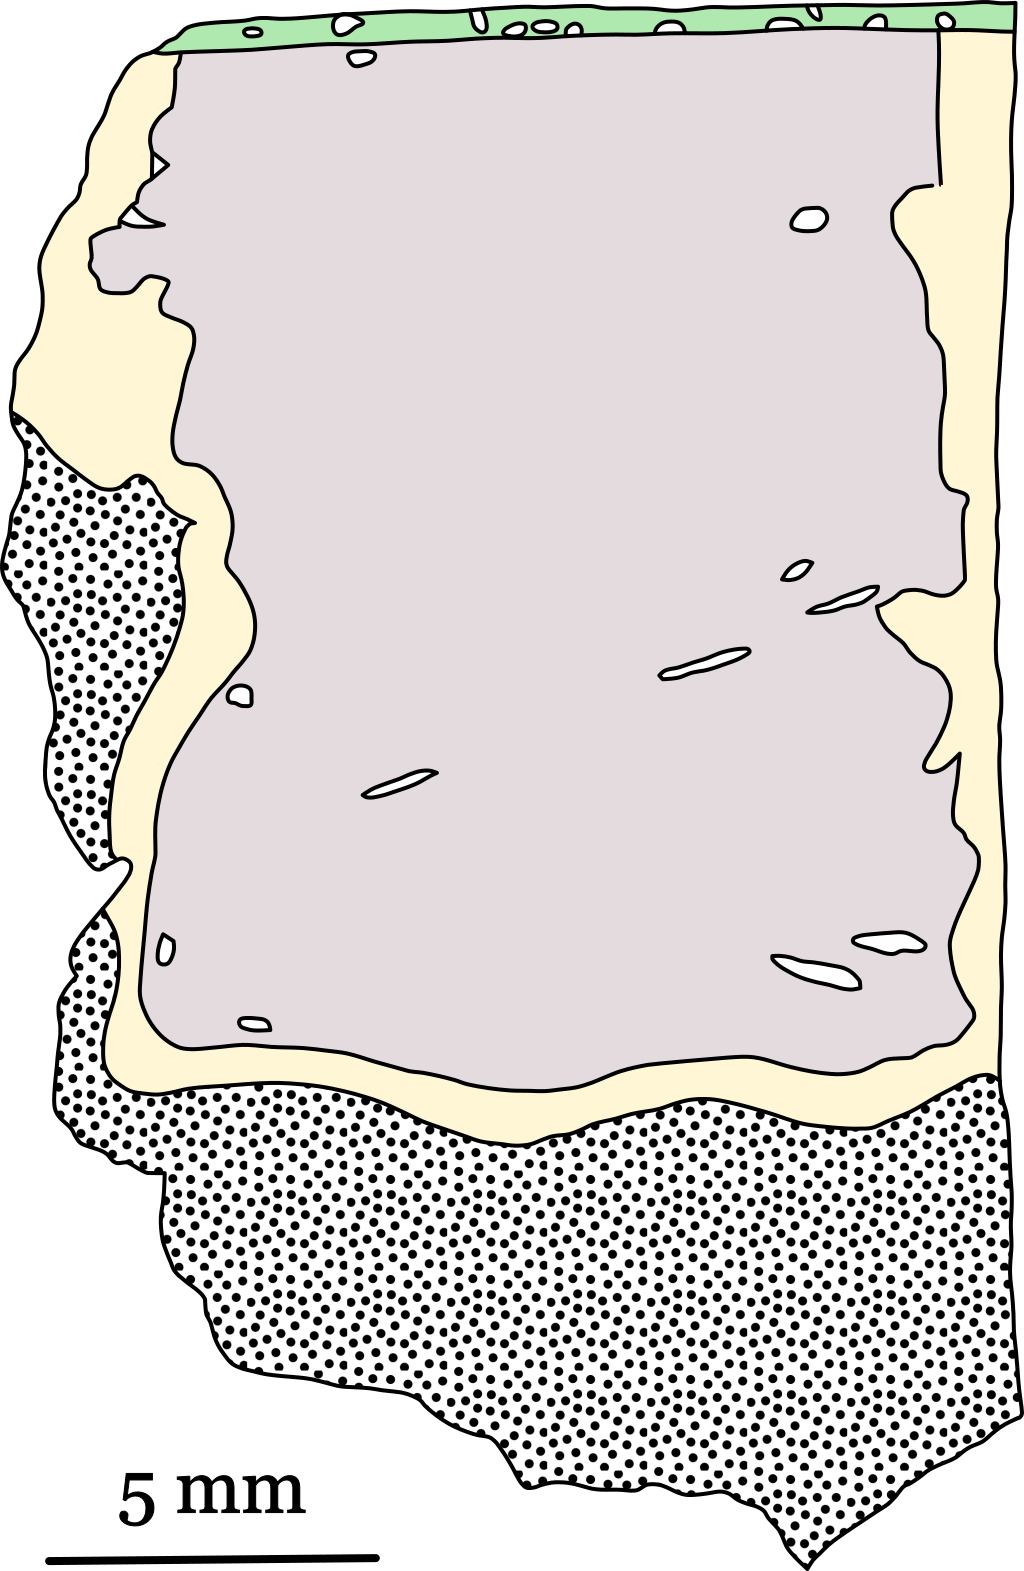
\includegraphics[scale=0.17]{PaM_BDX6528_lame}
    \subcaption{Lame étudiée \label{dessin:6528_lame}}

    \bigskip
    \bigskip

    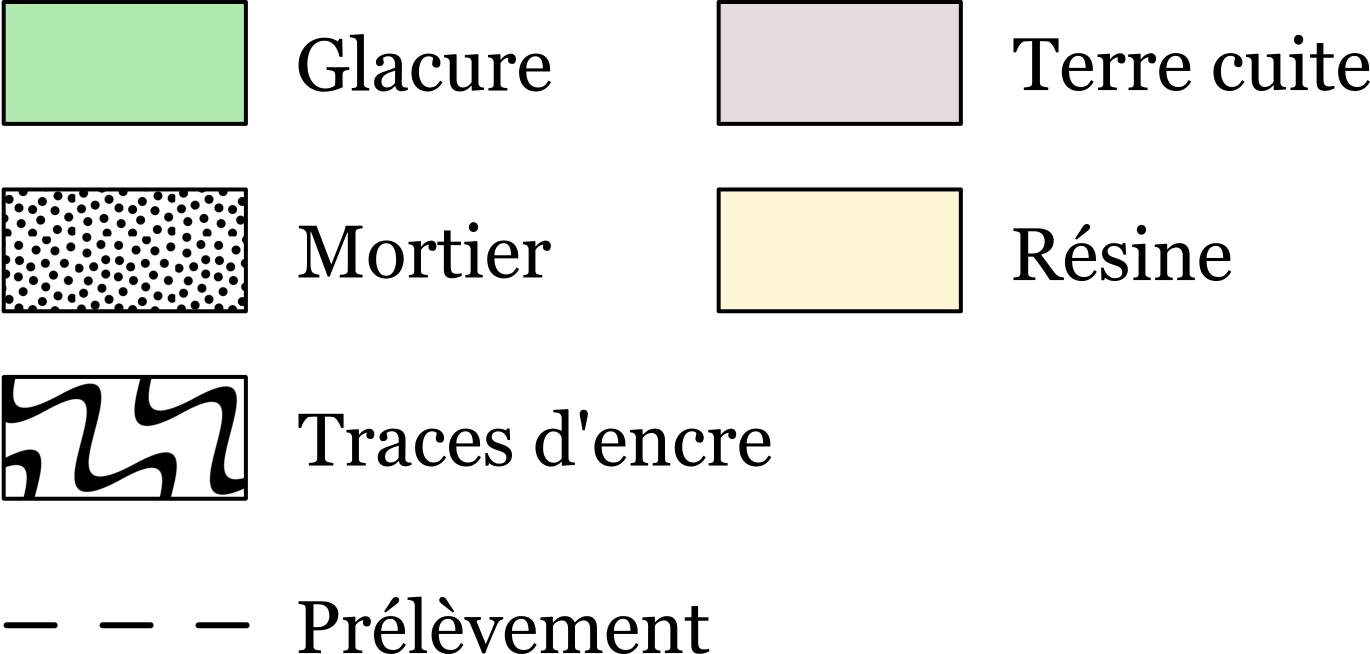
\includegraphics[scale=0.17]{PaM_BDX6528_legende}
  \end{minipage}
  \caption[\bdx{6528}]{\legendeA.}
  \label{dessin:6528}
\end{figure}

L'observation de la surface de la glaçure (\fref{surf:6528}) montre 
qu'elle contient des bulles, des picots, présente des rayures et 
contient des cristaux non fondus. On peut aussi remarquer des taches 
blanches, dues peut-être à une cristallisation en surface ou à un 
piquetage du verre.

Le support de terre cuite est de couleur rougeâtre, de granulométrie 
fine, peu poreux et contient de nombreuses inclusions de tailles et 
de couleurs variées.

\begin{figure}[htb]
% \begin{figure}[p]
  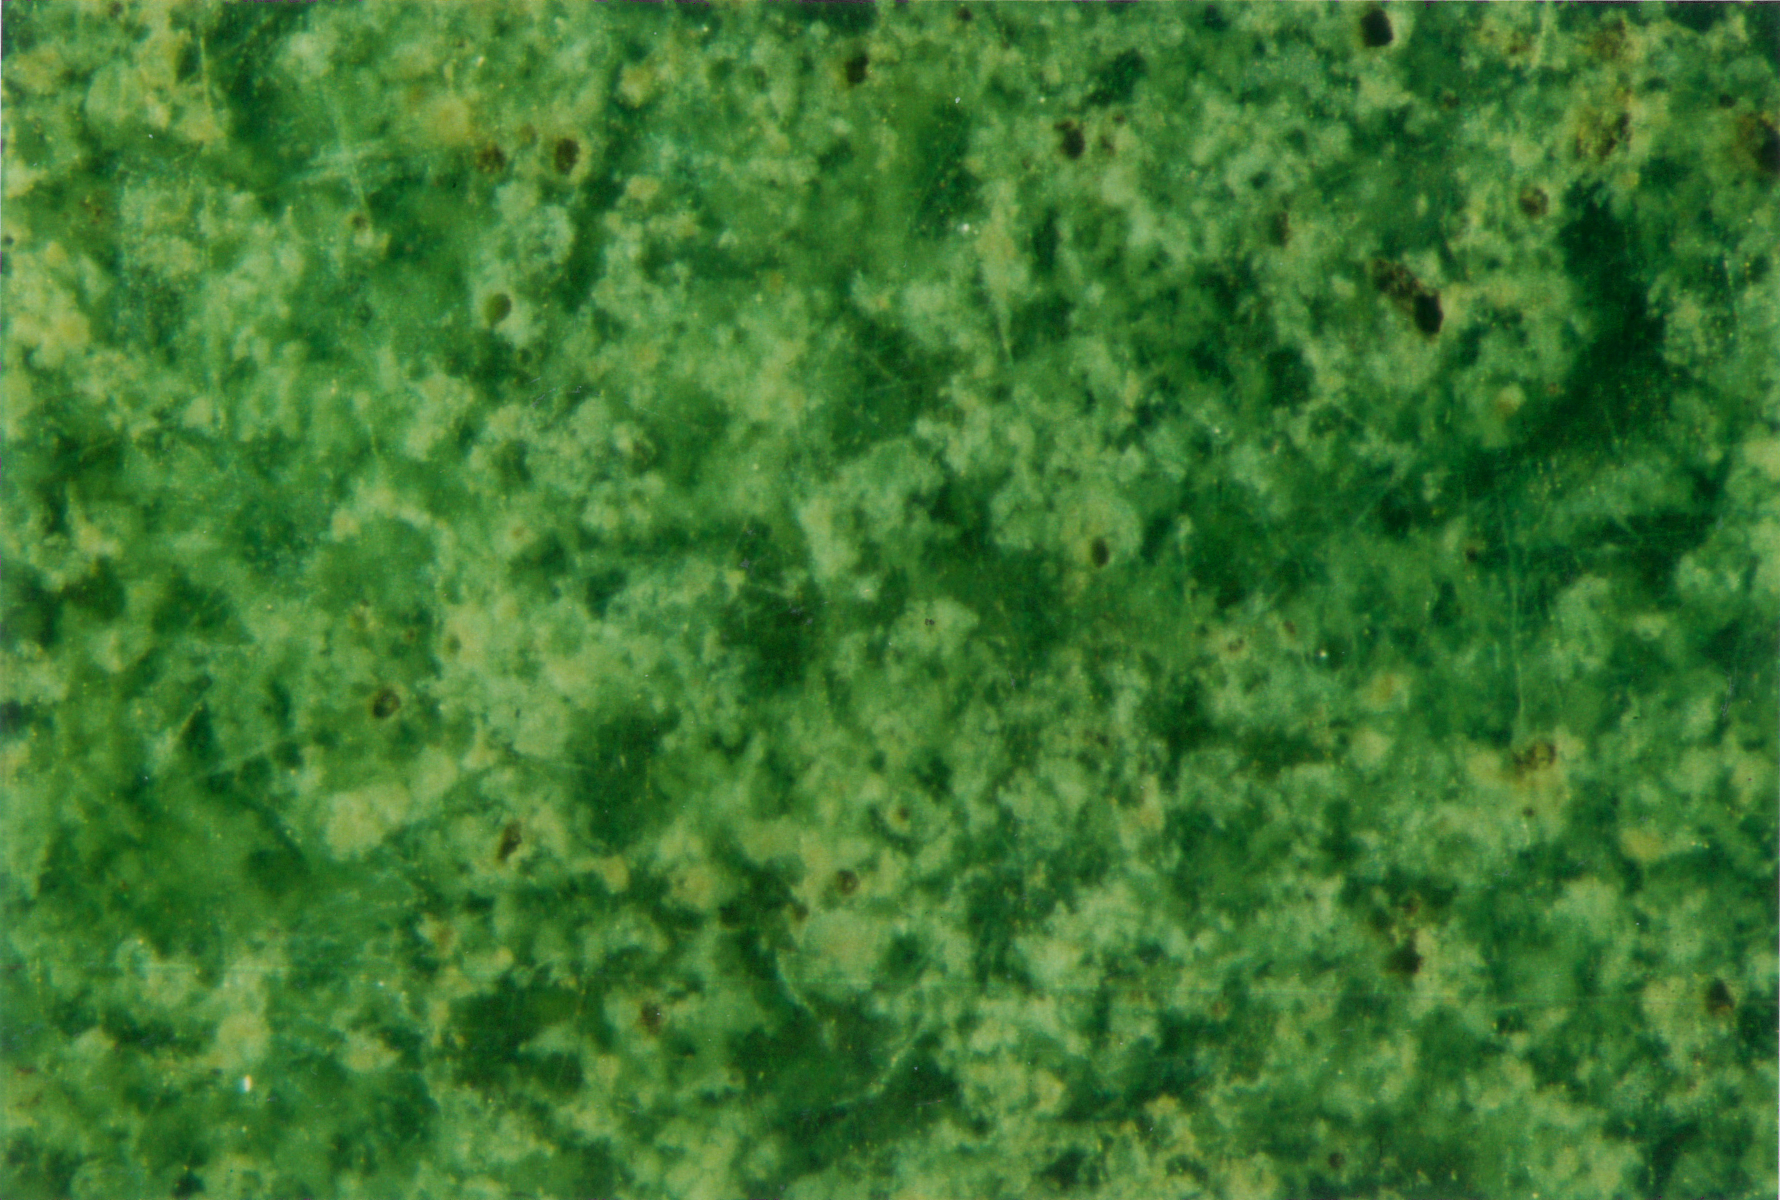
\includegraphics[width=\textwidth]{PaM_BDX6528_Surf}
  \caption[\bdx{6528}\ -- État de surface de la glaçure]
          {\legendeA.
           État de surface de la glaçure 
           (Gr=30, \zone{\sim4.3x3.2}{\mm}). 
           Elle contient des bulles, des picots, des cristaux 
           non fondus et présente des rayures.}
  \label{surf:6528}
\end{figure}


\section{Étude de la couleur}
%----------------------------------------------------------------------

\subsection{Identification des ions chromogènes}
%~~~~~~~~~~~~~~~~~~~~~~~~~~~~~~~~~~~~~~~~~~~~~~~~~~~~~~~~~~~~~~~~~~~~~~
Le spectre d'\AO en mode réflexion diffuse de la glaçure verte 
(\fref{spectre:6528}) présente une bande d'absorption large commençant 
à \SI{550}{nm} et dont le maximum se situe vers \SI{795}{nm}. Cette 
absorption est attribuable au \ch{Cu^2+} \autocite{Lajarte_1979}. On 
peut également distinguer un épaulement vers \SI{440}{nm} et un autre 
vers \SI{380}{nm} correspondant au \ch{Fe^3+}. La glaçure étant 
transparente, il peut s'agir d'une contribution de la terre cuite 
qui présente, elle aussi, ces absorptions (\fref{spectre:6528}). 
La présence de \ch{Fe^3+} peut expliquer la teinte légèrement jaune 
du vert de la glaçure.

\begin{figure}[htb]
% \begin{figure}[p]
  \begin{plotspectre}
    \addplot [thick, PaleGreen!66!black] 
       table [x=lambda, y=6528gla] {\gladata} ;
    \addlegendentry{glaçure verte}
    \addplot [thick, FireBrick] 
       table [x=lambda, y=6528tc] {\tcdata} ;
    \addlegendentry{terre cuite}

    \begin{scope}[<-, >=stealth, shorten <=5pt, thin]
      \node (Cu) at (780.00, 0.81) {\ch{Cu^2+}} ;
      \node (Fe) at (410.00, 0.32) {\ch{Fe^3+}} ;
      \node (qm) at (540.00, 0.20) {?} ;
      \draw (380.00, 0.59) |- (Fe.north) ;
      \draw (440.00, 0.48) |- (Fe.north) ;
      \draw (540.00, 0.35) |- (qm.north) ;
    \end{scope}
  \end{plotspectre}
  \caption[\bdx{6528}\ -- Spectres d'\AO en mode réflexion diffuse 
           de la glaçure et de la terre cuite]
          {\legendeA.
           Spectres d'\AO en mode réflexion diffuse de la glaçure et 
           de la terre cuite. La coloration verte de la glaçure est 
           due au \ch{Cu^2+} mis en évidence par la bande large à 
           partir de \SI{550}{\nm}. Le spectre de la terre cuite 
           présente deux bandes à \SIlist{380;440}{\nm}, attribuables 
           au \ch{Fe^3+} \autocite{Lajarte_1979}.}
  \label{spectre:6528}
\end{figure}

\subsection{Mesure physique de la couleur}
%~~~~~~~~~~~~~~~~~~~~~~~~~~~~~~~~~~~~~~~~~~~~~~~~~~~~~~~~~~~~~~~~~~~~~~
Les coordonnées \trichros correspondant aux espaces \Yxy et \Lab 
ont été obtenues à partir du spectre d'\AO{} (\tref{saotab:6528}). 
La longueur d'onde dominante obtenue pour la glaçure la place dans 
le domaine des vert-jaune \autocite{Kelly_1976}. La relativement 
faible réflectance \CIEY révèle une couleur assez foncée et la 
pureté d'excitation est celle d'une couleur peu saturée. La
\fref{colorfig:6528} présente la localisation des coordonnées 
chromatiques de la glaçure verte dans les espaces \Yxy et \Lab. 
La terre cuite a une longueur d'onde dominante de \SI{580.75}{\nm} 
qui la situe dans le domaine du jaune orange.

% \begin{table}[hbt]
\begin{table}[p]
  \caption[\bdx{6528}\ -- Coordonnées chromatiques et longueur d'onde 
           dominante]
          {\legendeA.
           Coordonnées chromatiques dans les systèmes \Yxy et \Lab 
           et longueur d'onde dominante (illuminant D65, \ang{2},
           \SIrange{400}{700}{\nm}). (\up{\dag}\,\cite{Kelly_1976})}
  \label{saotab:6528}
  \begin{chrotab}
      \chrolgna{Glaçure}{563.41}{20.39}
               {28.102}{0.330}{0.384}
               {59.981}{-10.927}{15.673} &
      \chrolgnb{vert jaune foncé}{Vert-Jaune}{560}{570}{}
               % {\footnotemark{}}
    \tabularnewline
      \chrolgna{Terre cuite}{580.75}{21.53}
               {47.846}{0.357}{0.362}
               {74.728}{4.772}{16.629} &
      \chrolgnb{jaune orange clair}{Jaune-Orange}{580}{585}{}
               % {\footnotemark{}}
    \tabularnewline
  \end{chrotab}
\end{table}
% \addtocounter{footnote}{-1}
% \footnotetext{\autocite{Kelly_1976}}
% \addtocounter{footnote}{+1}
% \footnotetext{\autocite{Kelly_1976}}

% \begin{figure}[htb]
\begin{figure}[p]
  \newcommand{\samplename}{6528gla}
  \newcommand{\samplecolor}{PaleGreen}
  \begin{minipage}[t]{0.37\paperwidth}
    \begin{plotYxy}
      \plotYxyPaV ;
      \plotYxyIlluminant ;
      \plotYxySample{\samplename}{\samplecolor} ;
      \plotYxyLigne{\samplename} ;
      \plotYxyAnnot{\samplename}{south west} ;
    \end{plotYxy}
    \subcaption[Espace \trichro \Yxy]
               {Espace \trichro \Yxy. La longueur d'onde 
                dominante de la glaçure est \SI{563.413}{\nm}. 
                Elle est dans le domaine de vert-jaune. Le point 
                représentatif est proche de l'illuminant standard, 
                la couleur est peu saturée.}
  \end{minipage}%
  \qquad%
  \begin{minipage}[t]{0.37\paperwidth}
    \begin{plotLab}
      \plotLabSample{\samplename}{\samplecolor} ;
    \end{plotLab}
    \subcaption[Espace \trichro \Lab]
               {Espace \trichro \Lab. Le point représentatif 
                de la couleur de la glaçure est dans le quart 
                vert-jaune.}
  \end{minipage}%
  \caption[\bdx{6528}\ -- Analyse chromamétrique de la glaçure]
          {\legendeA. Analyse chromamétrique de la glaçure.}
  \label{colorfig:6528}
\end{figure}


\section{Étude de la texture de la glaçure et de la terre cuite sur 
         une section polie}
%----------------------------------------------------------------------

\subsection{Observation en lumière naturelle}
%~~~~~~~~~~~~~~~~~~~~~~~~~~~~~~~~~~~~~~~~~~~~~~~~~~~~~~~~~~~~~~~~~~~~~~
\begin{figure}[htb]
  \begin{minipage}[t]{0.48\textwidth}
    \fakeimg{lum. nat.}
    \subcaption{Lumière naturelle \label{texture:6528_LN}}
  \end{minipage}%
  \hfill%
  \begin{minipage}[t]{0.48\textwidth}
    \fakeimg{Cathodo}
    \subcaption{\CL \label{texture:6528_CL}}
  \end{minipage}
  \caption[\bdx{6528}\ -- Observation de la texture en section]
          {\legendeA.
           Observation de la texture en section 
           sur une surface de \SI{2.6x1.9}{\mm}.}
  \label{texture:6528}
\end{figure}

L'examen d'une section en lumière naturelle 
(\fref{texture:6528_LN}) montre que la glaçure est colorée dans 
la masse et qu'elle adhère bien au support de terre cuite. La terre 
cuite contient de nombreuses inclusions de tailles et de couleurs 
diverses, réparties de manière homogène.

La limite entre la glaçure et le support de céramique semble 
particulièrement nette.

\subsection{Observation en \CL}
%~~~~~~~~~~~~~~~~~~~~~~~~~~~~~~~~~~~~~~~~~~~~~~~~~~~~~~~~~~~~~~~~~~~~~~
La glaçure n'est pas luminescente (\fref{texture:6528_CL}).

La terre cuite présente une luminescence mauve et contient des 
inclusions qui luminescent en rouge ou bleu, réparties de manière 
homogène dans l'ensemble du matériau.

À l'interface terre cuite-glaçure, on observe un très faible liseré 
qui luminescence en bleu.

\subsection{Observation en \MEB[ie]}
%~~~~~~~~~~~~~~~~~~~~~~~~~~~~~~~~~~~~~~~~~~~~~~~~~~~~~~~~~~~~~~~~~~~~~~
La glaçure a une épaisseur moyenne de \SI{350}{\um}. Elle contient des 
bulles. On peut également distinguer des cristaux de néoformation dans 
sa masse et à l'interface glaçure-terre cuite 
(\fref{MEB:6528_img}).

Une \carto de \RX (\fref{MEB:6528_carto_tcgla}) a permis de distinguer 
la présence de cristaux non fondus de quartz dans la glaçure. Celle-ci 
est également riche en plomb et contient du cuivre. Elle est en 
revanche moins riche en calcium et aluminium que la terre cuite.

% \begin{figure}[htb]
\begin{figure}[p]
  \fakeimg{Texture au MEB, retrodiff (fig 23)}
  \caption[\bdx{6528}\ -- Observation de la texture au \MEB, 
           en mode \ERD. Ensemble glaçure/terre cuite]
          {\legendeA.
           Observation de la texture au \MEB, en mode \ERD. 
           Ensemble glaçure/terre cuite. La barre d'échelle mesure 
           \SI{200}{\um} (\zone{650x530}{\um}).}
  \label{MEB:6528_img}
\end{figure}

L'interface glaçure-terre cuite semble être riche en potassium et 
calcium. Son faible développement laisse supposer des interactions 
faibles entre ces deux matériaux  et peut donc faire envisager 
l'hypothèse d'une application de la glaçure sur une terre cuite.

La terre cuite contient des inclusions 
(\SIrange[range-phrase=\ à\ ]{50}{150}{\um}), identifiées par \carto 
de \RX (\fref{MEB:6528_carto_tc}), comme des cristaux de quartz et de 
feldspaths potassiques et sodiques. La présence de ces derniers peut 
être corrélée avec les luminescences ponctuelles bleues détectées en 
\CL. Le calcium présent dans toute la terre cuite peut être 
responsable, sous forme de calcite, des luminescences rouges détectées 
en \CL.

\noindent Remarque : le mauvais état de surface de la lame est dû aux 
contraintes mécaniques qu'elle subit lors du sciage et du polissage.

% \begin{figure}[htb]
\begin{figure}[p]
  \fakeimg{Texture au MEB, carto tc/gla (fig 24)}
  \caption[\bdx{6528}\ -- Observation de la texture au \MEB, 
           \carto de \RX de l'ensemble glaçure-terre cuite]
          {\legendeA.
           Observation de la texture au \MEB, 
           \carto de \RX de l'ensemble glaçure-terre cuite 
           (Gr=150, \zone{735x600}{\um}).}
  \label{MEB:6528_carto_tcgla}
\end{figure}

% \begin{figure}[htb]
\begin{figure}[p]
  \fakeimg{Texture au MEB, carto tc (fig 25)}
  \caption[\bdx{6528}\ -- Observation de la texture au \MEB, 
           \carto de \RX de la terre cuite]
          {\legendeA.
           Observation de la texture au \MEB, 
           \carto de \RX de la terre cuite 
           (Gr=190, \zone{580x475}{\um}).}
  \label{MEB:6528_carto_tc}
\end{figure}


\section{Composition élémentaire de la glaçure}
%----------------------------------------------------------------------

% \begin{table}[hbt]
\begin{table}[p]
  \caption[\bdx{6528}\ -- Analyse quantitative par \EDS, 
           composition élémentaire de la glaçure]
          {\legendeA. Analyse quantitative par \EDS. Composition 
           élémentaire de la glaçure verte sur une surface de 
           \SI{108x88}{\um} (\PMO).}
  \label{compelem:6528_gla}
  \begin{cartotab}
      \cartolgn{SiO2}{36.55}{3.79} &
      \cartolgn{CaO}{2.43}{0.23}   &
      \cartolgn{Al2O3}{2.37}{0.18} &
      \cartolgn{MgO}{0.67}{0.08}
    \tabularnewline
      \cartolgn{Na2O}{0.34}{0.02}  &
      \cartolgn{K2O}{0.91}{0.10}   &
      \cartolgn{Fe2O3}{1.13}{0.09} &
      \cartolgn{PbO}{54.49}{4.05}
    \tabularnewline
      \cartolgnnd{SnO2}          &
      \cartolgn{CuO}{0.72}{0.09} &
      \cartolgnnd{CoO}           &
      \cartolgnnd{MnO}
    \tabularnewline
      \cartolgnnd{Cr2O3} &
      \cartolgnnd{ZnO}   &
      \cartolgnnd{Sb2O3} &
      \cartolgn{TiO2}{0.15}{0.06}
    \tabularnewline
      \cartolgnnd{S}            &
      \cartolgnnd{P2O5}         &
      \cartolgn{Cl}{0.25}{0.05} &
      \cartolgnnd{As2O3}
    \tabularnewline
  \end{cartotab}
\end{table}

Le \tref{compelem:6528_gla} présente la composition élémentaire de 
la glaçure blanche obtenue par \EDS. Ils sont donnés en pourcentages 
massiques d'oxyde normalisés à \SI{100}{\percent}. Ce sont des 
moyennes de trois à cinq mesures effectuées sur toute la longueur 
de la glaçure, sur la zone d'analyse la plus grande possible, et en 
prenant garde d'éviter les bulles et cristaux non fondus. Il en est 
de même pour toutes les compositions élémentaires présentées dans ce 
mémoire.

Il s'agit d'une glaçure plombifère transparente. La présence de 
cuivre (\SI{0.72}{\percent} de \ch{CuO}), détecté également en \SAO 
sous la forme \ch{Cu^2+}, est responsable de sa couleur verte. Elle 
est très légèrement teintée de jaune, probablement à cause de la 
présence de \ch{Fe^3+} (\SI{1.13}{\percent} de \ch{Fe2O3}).


\section{Étude de la terre cuite support}
%----------------------------------------------------------------------

\subsection{Composition élémentaire}
%~~~~~~~~~~~~~~~~~~~~~~~~~~~~~~~~~~~~~~~~~~~~~~~~~~~~~~~~~~~~~~~~~~~~~~
Comme pour la glaçure, les résultats sont présentés en pourcentages 
massiques d'oxyde et sont des moyennes de trois à cinq mesures 
réparties dans l'ensemble de la terre cuite (\tref{compelem:6528_tc}).

La terre cuite est riche en calcium (\SI{20.30}{\percent} 
de \ch{CaO}). Sa coloration ocre rosé est due au \ch{Fe^3+} 
(\SI{7.18}{\percent} de \ch{Fe2O3}) en atmosphère de cuisson oxydante 
\autocite{Echallier_1984}.

% \begin{table}[hbt]
\begin{table}[p]
  \caption[\bdx{6528}\ -- Analyse quantitative par \EDS, 
           composition élémentaire de la terre cuite]
          {\legendeA. Analyse quantitative par \EDS. 
           Composition élémentaire de la terre cuite 
           sur une surface de \SI{2160x1752}{\um} (\PMO).}
  \label{compelem:6528_tc}
  \begin{cartotab}
      \cartolgn{SiO2}{53.71}{2.42} &
      \cartolgn{CaO}{20.30}{1.22} &
      \cartolgn{Al2O3}{12.58}{0.68} &
      \cartolgn{MgO}{3.10}{0.24}
    \tabularnewline
      \cartolgn{Na2O}{0.63}{0.05} &
      \cartolgn{K2O}{1.53}{0.07} &
      \cartolgn{Fe2O3}{7.18}{0.65} &
      \cartolgnnd{PbO} 
    \tabularnewline
      \cartolgnnd{SnO2} &
      \cartolgnnd{CuO} &
      \cartolgnnd{CoO} &
      \cartolgnnd{MnO} 
    \tabularnewline
      \cartolgnnd{Cr2O3} &
      \cartolgnnd{ZnO} &
      \cartolgnnd{Sb2O3} &
      \cartolgn{TiO2}{0.68}{0.04}
    \tabularnewline
      \cartolgn{S}{0.19}{0.03} &
      \cartolgnnd{P2O5} &
      \cartolgn{Cl}{0.09}{0.02} &
      \cartolgnnd{As2O5} 
    \tabularnewline
  \end{cartotab}
\end{table}

La présence de calcium dans une argile favorise l'attaque, à haute 
température, des silicates pour former des phases telles que la 
gehlénite ou le diopside. La gehlénite peut piéger les ions ferreux 
ou ferriques et empêcher ainsi la formation, en atmosphère oxydante, 
de l'hématite (\ch{Fe2O3}) qui donne à la céramique sa coloration 
plus ou moins rouge. Ici, on peut supposer que tout le fer présent 
dans l'argile de départ n'a pas été piégé par les phases haute 
température et que cet excès est responsable de la coloration de 
la terre cuite.

\subsection{Composition \cristallo}
%~~~~~~~~~~~~~~~~~~~~~~~~~~~~~~~~~~~~~~~~~~~~~~~~~~~~~~~~~~~~~~~~~~~~~~
% \begin{figure}[htb]
\begin{figure}[p]
  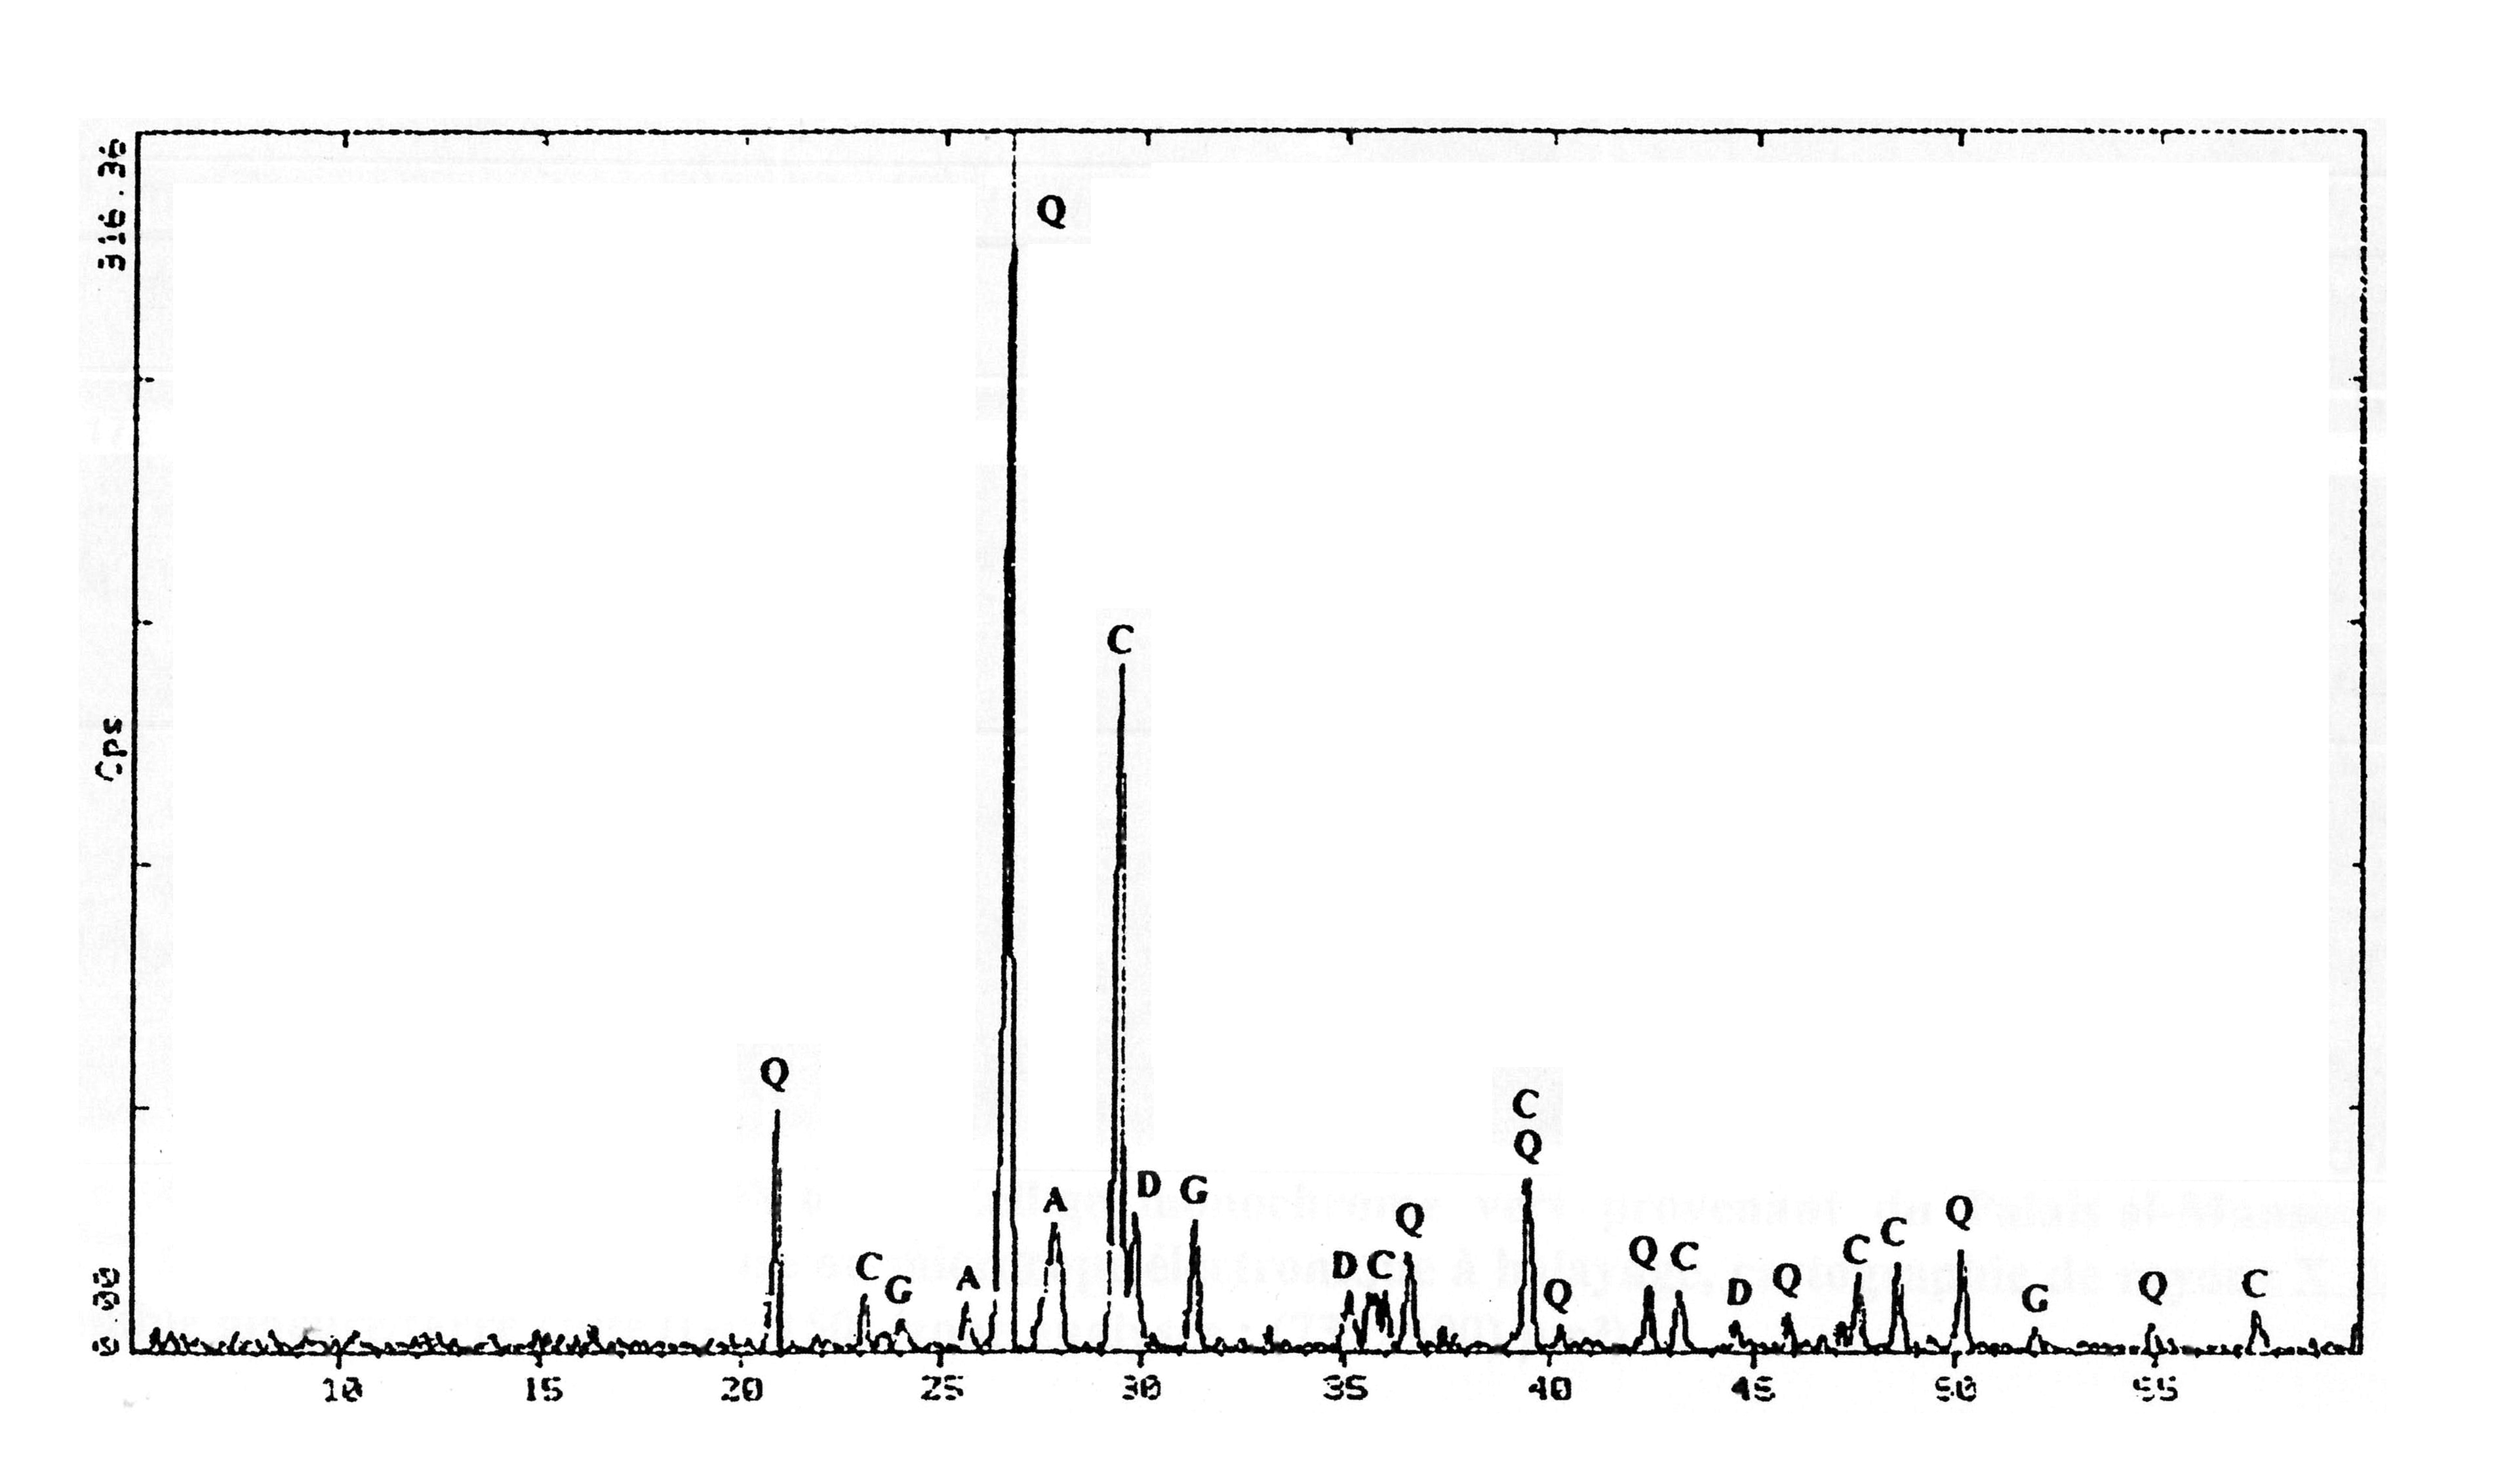
\includegraphics[width=\textwidth]{PaM_BDX6528_DX}
  \caption[\bdx{6528}\ -- Diffraction de \RX sur poudre 
           de la terre cuite]
          {\legendeA.
           \DX[D] sur poudre de la terre cuite. 
           Mise en évidence de la présence de quartz (Q), 
           calcite (C), gehlénite (G), anorthite (A), diopside (D).}
  \label{DRX:6528}
\end{figure}

La principale phase cristalline mise en évidence par \DX sur 
poudre (\fref{DRX:6528}) est le quartz (\quartz), responsable de la 
luminescence mauve de la terre cuite. On note également la présence de 
calcite (\calcite) qui peut être associée aux luminescences rouges 
détectées en \CL. Enfin, La terre cuite contient également des phases 
haute température telles que le diopside alumineux (\diopsidealfe), la 
gehlénite (\gehlenite) et l'anorthite (\anorthite). Les luminescences 
bleues détectées en \CL peuvent être associées à la présence de 
diopside et de gehlénite.

La présence de ces phases haute température laisse penser 
que la température de cuisson de la terre cuite aurait atteint 
\SIrange[range-phrase=\ à\ ]{900}{950}{\degC}.


\section{Sur la présence et l'identification de cristaux de 
         dévitrification}
%----------------------------------------------------------------------

On distingue, dans la masse de la glaçure et dans la zone d'interface 
entre celle-ci et la terre cuite, des cristaux de forme polygonale 
(\fref{MEB:6528_img_cx}). Ce sont des cristaux de dévitrification. 
Ils se développent pendant le refroidissement lent de la glaçure à 
partir de germes formés à haute température. Des analyses ponctuelles 
(\tref{compelem:6528_cx}) et une \carto de \RX ont montré qu'il s'agit 
de silicates de magnésium et de calcium.

\begin{figure}[htb]
  \fakeimg{6528ER96}
  \caption[\bdx{6528}\ -- Image en mode \ERD, cristaux de 
           dévitrification de forme polygonale]
          {\legendeA.
           Observation au \MEB, image en mode \ERD. Cristaux de 
           dévitrification de forme polygonale. La barre d'échelle 
           mesure \SI{10}{\um} \zone{33x27}{\um}.}
  \label{MEB:6528_img_cx}
\end{figure}

% \begin{table}[hbt]
\begin{table}[p]
  \caption[\bdx{6528}\ -- Analyse quantitative par \EDS, 
           composition élémentaire des cristaux de dévitrification]
          {\legendeA. Analyse quantitative par \EDS. 
           Composition élémentaire des cristaux de dévitrification 
           par analyses ponctuelles (\SI{1}{\um\squared}) (\PMO).}
  \label{compelem:6528_cx}
  \begin{cartotab}
      \cartolgn{SiO2}{50.12}{3.37} &
      \cartolgn{CaO}{16.80}{2.58}  &
      \cartolgn{Al2O3}{2.73}{1.39} &
      \cartolgn{MgO}{21.95}{3.09}
    \tabularnewline
      \cartolgnnd{As2O5} &
      \cartolgnnd{Na2O}  &
      \cartolgnnd{K2O}   &
      \cartolgn{Fe2O3}{3.94}{2.24} 
    \tabularnewline
      \cartolgn{PbO}{3.88}{0.90} &
      \cartolgnnd{SnO2} &
      \cartolgn{CuO}{0.30}{0.23} &
      \cartolgnnd{CoO}
    \tabularnewline
      \cartolgnnd{MnO} &
      \cartolgnnd{Cr2O3} &
      \cartolgnnd{ZnO} &
      \cartolgnnd{Sb2O3}
    \tabularnewline
      \cartolgn{TiO2}{0.23}{0.07} &
      \cartolgn{S}{0.12}{0.04} &
      \cartolgnnd{P2O5} &
      \cartolgnnd{Cl}
    \tabularnewline
  \end{cartotab}
\end{table}

Ces analyses élémentaires doivent être considérées avec prudence : 
en effet, les faibles dimensions de ces cristaux 
(\SIrange[range-phrase=\ à\ ]{1}{2}{\um} dans leur plus petite 
dimension) ne permettent pas de certifier que la glaçure avoisinante 
n'entre pas en compte dans les analyses.


\section{Étude des altérations de la glaçure}
%----------------------------------------------------------------------

Aucune figure d'altération n'a été mise en évidence dans la glaçure, 
ni visuellement, ni en \MEB[ie] (MEB).


\section{Bilan}
%----------------------------------------------------------------------

Cet échantillon est donc une pièce de céramique portant une 
glaçure plombifère dont la coloration verte est due au \ch{Cu^2+} 
en atmosphère de cuisson oxydante.

Son support de terre cuite est de type calcique. Sa coloration 
ocre-rose est due à la présence de \ch{Fe^3+} en atmosphère de 
cuisson oxydante.

Sa composition \cristallo (quartz, calcite, diopside, 
gehlénite, anorthite) laisse penser qu'elle a été cuite à une 
température de l'ordre de 
\SIrange[range-phrase=\ à\ ]{900}{950}{\degC}.

A l'interface glaçure-terre cuite, on distingue un très fin liseré 
présentant une luminescence bleue, associé à la présence de cristaux 
de dévitrification identifiés comme des silicates de magnésium et de 
calcium. Le faible développement de cette zone laisse envisager 
l'application du mélange glaçurant sur une terre cuite.

La glaçure ne présente pas de figure d'altération d'origine chimique 
mais une usure mécanique de surface.

%!TEX root = MemoireZelliges.tex

\chapter{Étude physique d'un zellige bleu verdâtre (\bdx{6529})}
%======================================================================

\section{Description -- État de surface}
%----------------------------------------------------------------------

Il s'agit d'un zellige provenant du \PaM, \siecle{17}, (Meknès, 
Maroc). De forme parallélépipédique, il comporte une glaçure bleu vert 
(\fref{dessin:6529}). Beaucoup plus épais et plus grand que les quatre 
autres échantillons, il est aussi le seul à ne pas être chanfreiné. 
On remarque également des coulures de la glaçure sur ses bords. Les 
traces d'encre sont dues à l'indexation de l'échantillon au Maroc.

Il s'agirait en fait, non pas d'un élément du décor de zelliges, mais 
plutôt d'un carreau utilisé pour le cerner. La présence de coulures 
indique que l'échantillon n'a pas subi de découpe après cuisson et 
leur répartition homogène sur ses quatre faces montre qu'il a été cuit 
à plat.

\begin{itemize}
  \item \DimText : \SI{75x59x39}{\mm}
  \item \emph{Masse} : \SI{257.1}{\g}
\end{itemize}

\begin{figure}[htb]
  \begin{minipage}[t]{8.8cm}
    \centerfloat
    % \RaggedLeft
    \vspace*{0pt}
    % Dessin de l'échantillon : Vue de dessus
    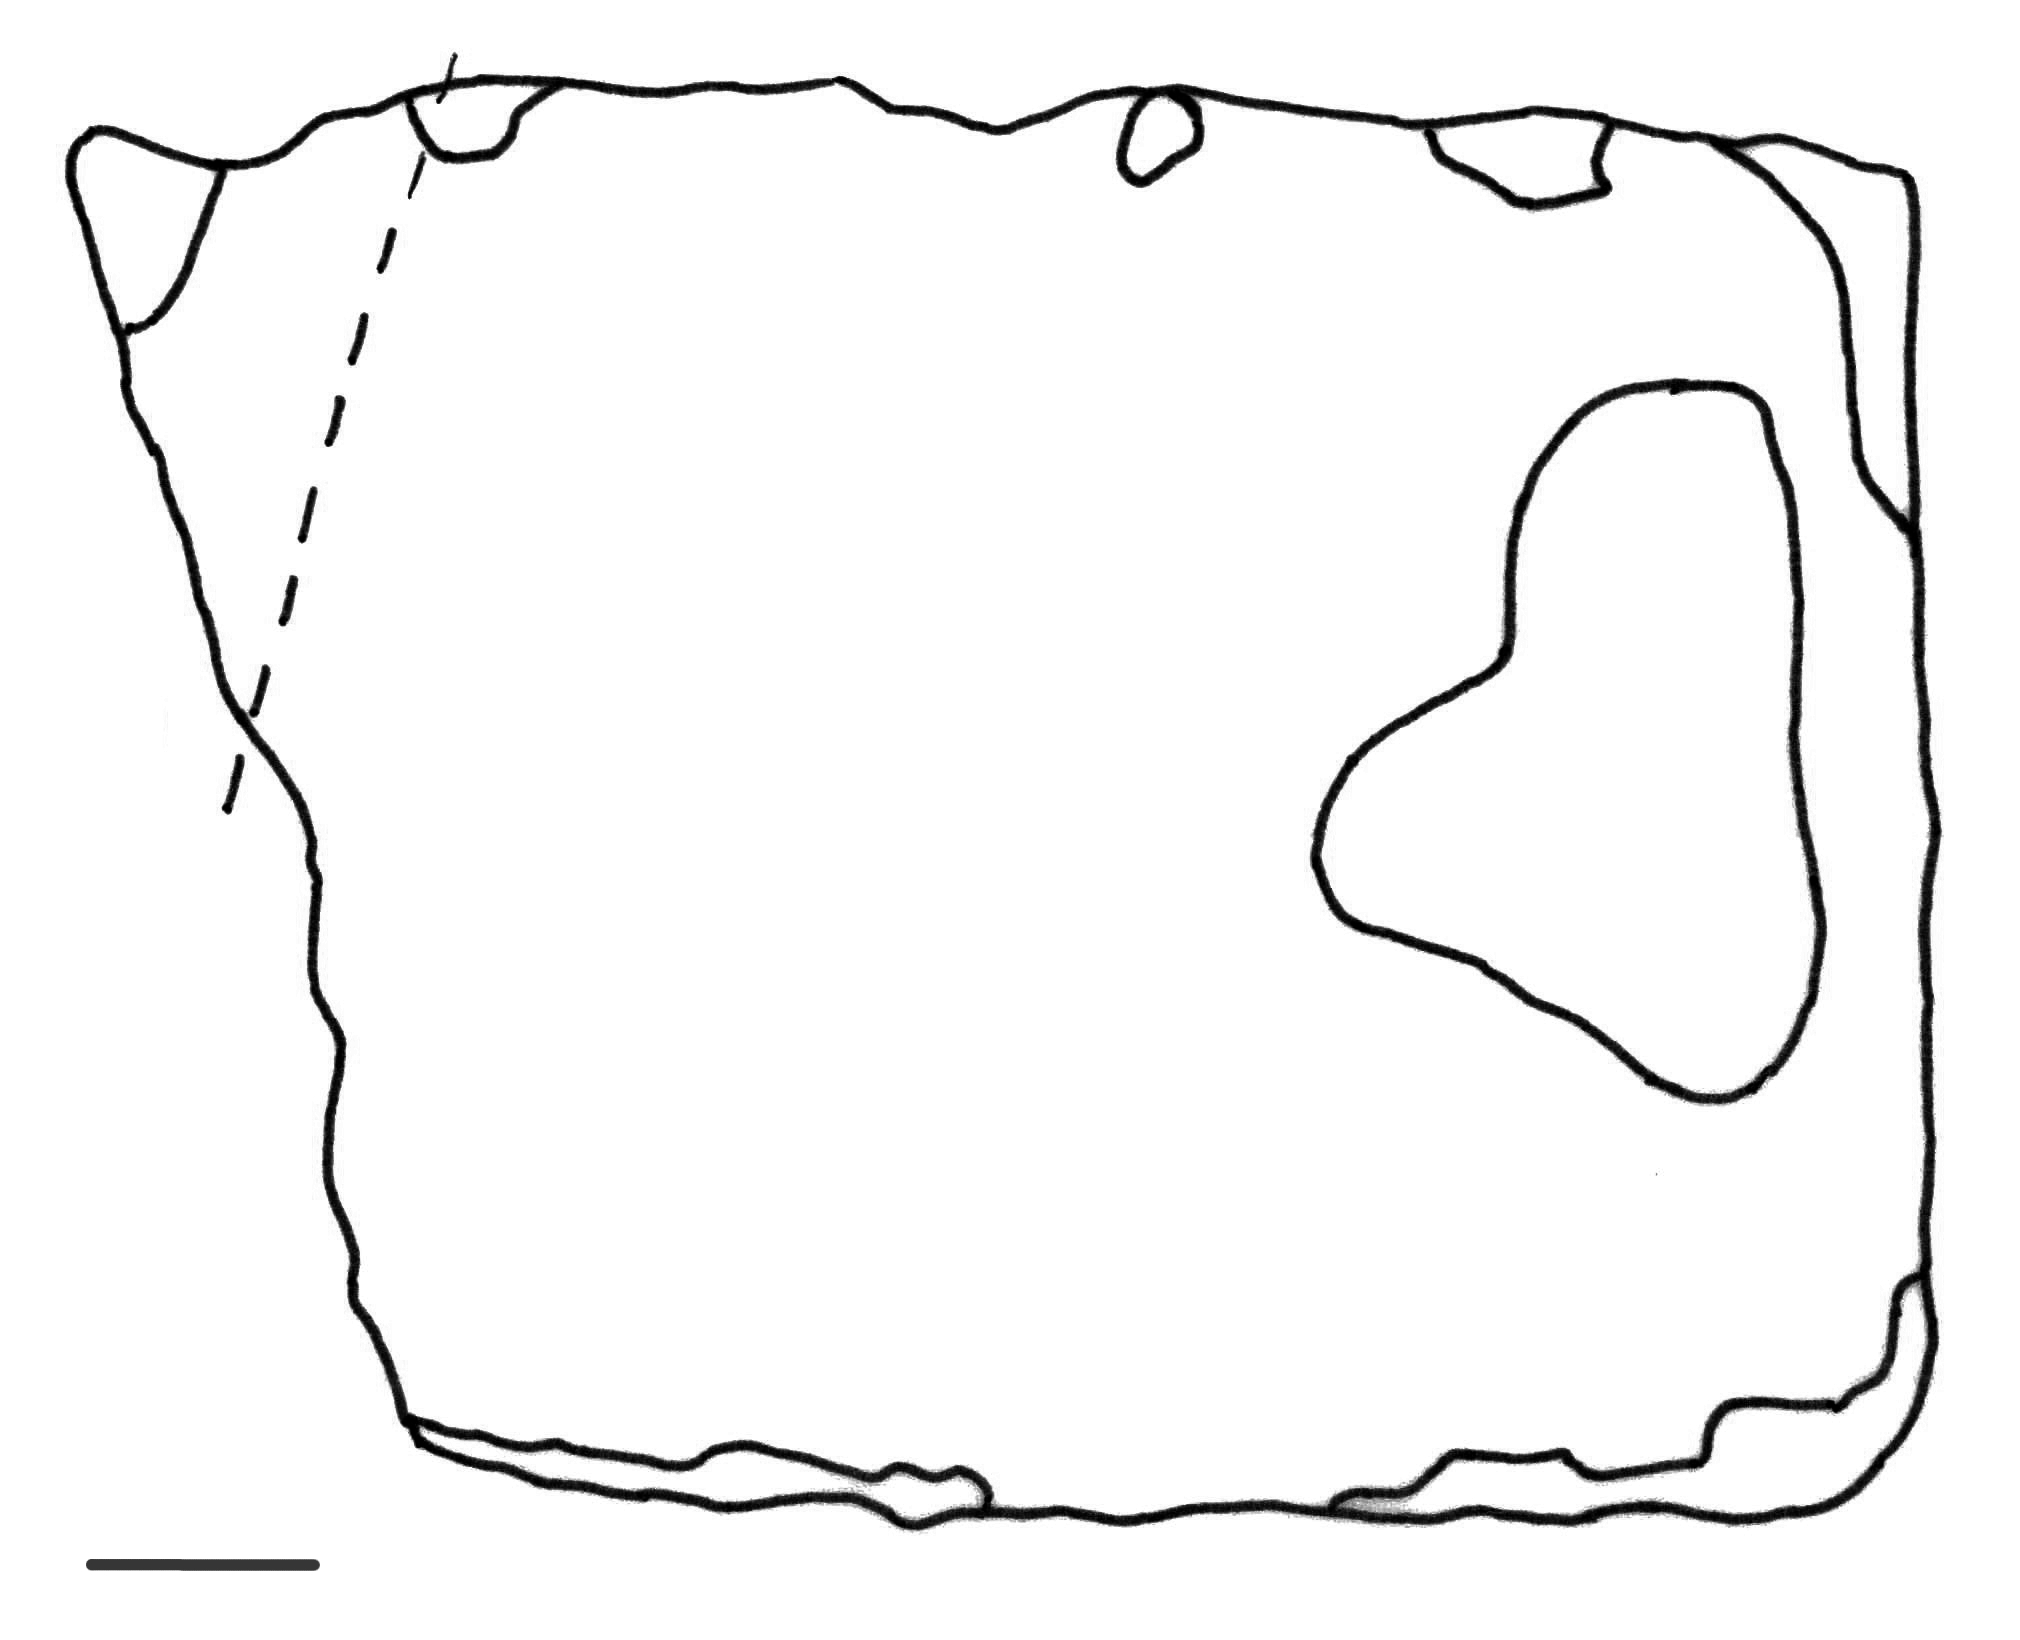
\includegraphics[scale=0.17]{PaM_BDX6529_dessus}
    \subcaption{Vue de dessus \label{dessin:6529_dessus}}

    \bigskip
    \bigskip

    % Dessin de l'échantillon : Coupe
    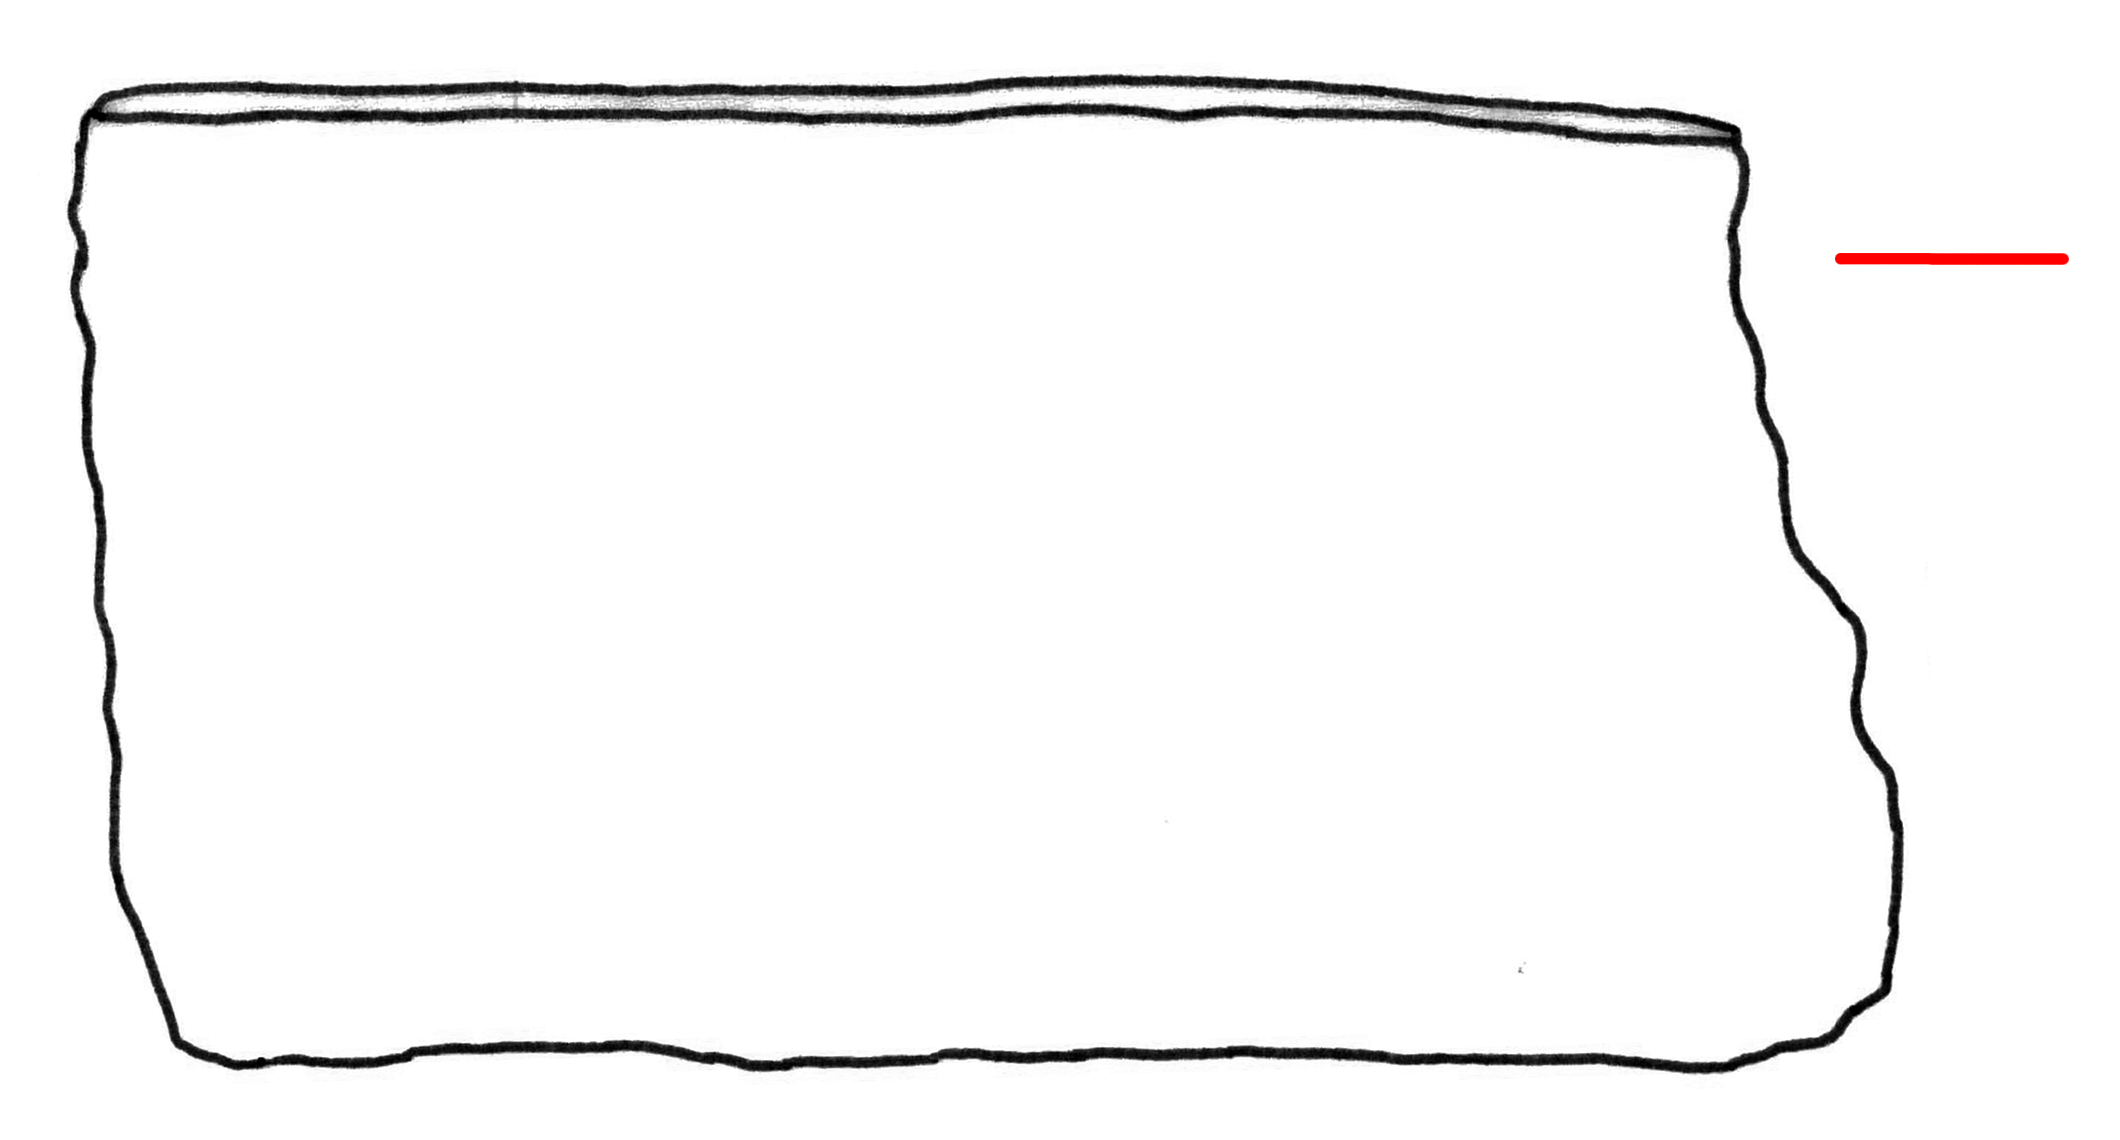
\includegraphics[scale=0.17]{PaM_BDX6529_coupe}
    \subcaption{Vue en coupe \label{dessin:6529_coupe}}
  \end{minipage}%
  \qquad%
  \begin{minipage}[t]{6.2cm}
    \centerfloat
    \vspace*{0pt}
    % Dessin de l'échantillon : Lame
    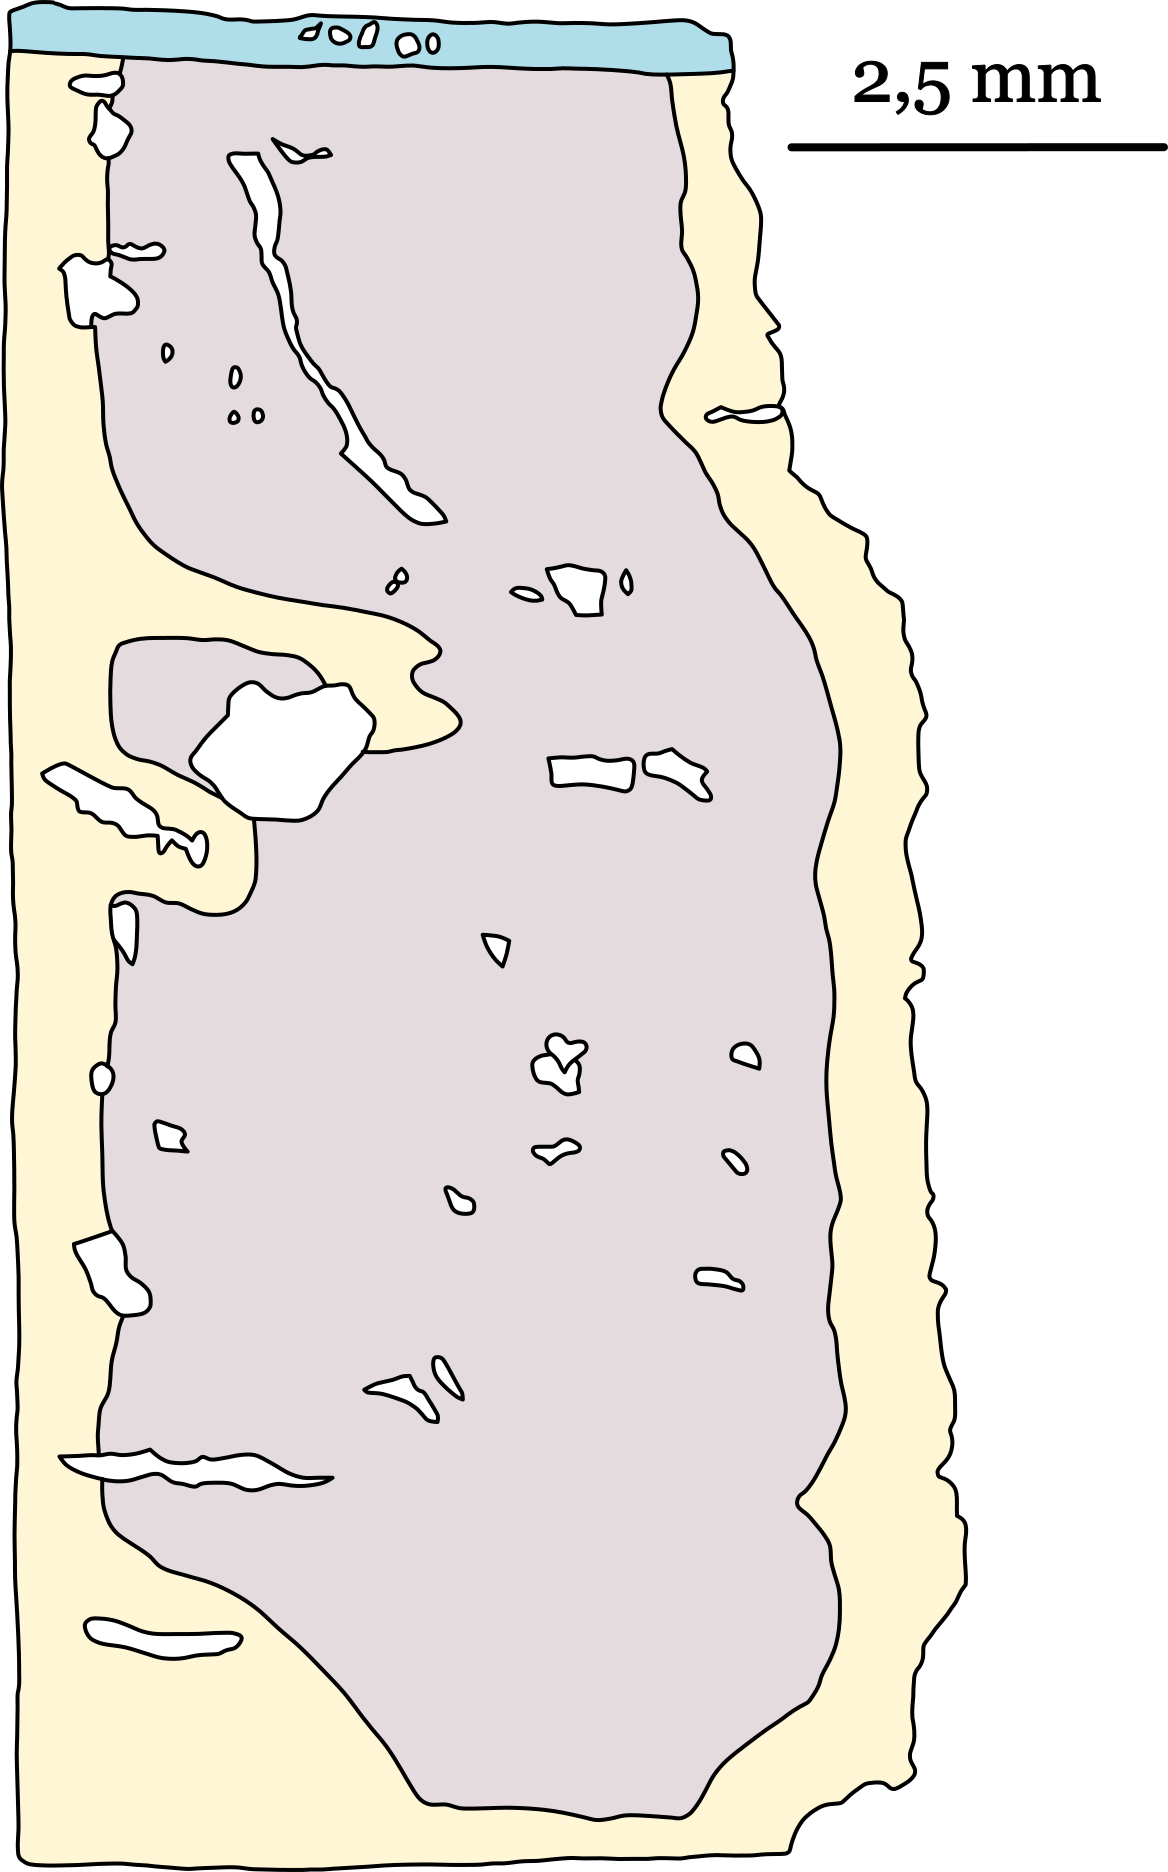
\includegraphics[scale=0.17]{PaM_BDX6529_lame}
    \subcaption{Lame étudiée \label{dessin:6529_lame}}

    \bigskip
    \bigskip
    \bigskip

    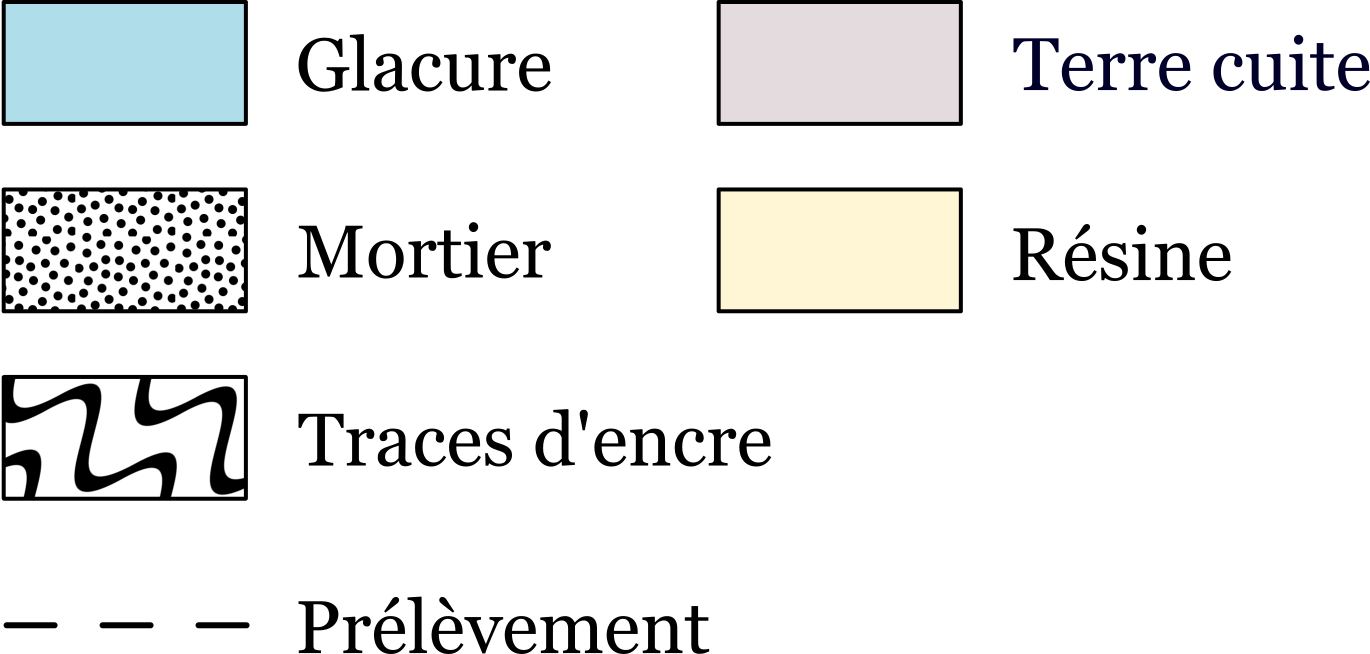
\includegraphics[scale=0.17]{PaM_BDX6529_legende}
  \end{minipage}
  \caption[\bdx{6529}]{\legendeB.}
  \label{dessin:6529}
\end{figure}

L'observation de la surface de la glaçure (\fref{surf:6529}) montre 
qu'elle est opaque et contient des bulles. Elle présente également 
une forte usure mécanique pouvant s'expliquer par le fait que 
l'échantillon provient d'un pavement de sol.

Le support de terre cuite est de couleur rougeâtre, de granulométrie 
fine, et contient quelques porosités de grande taille ainsi que des 
inclusions rouges et blanches.

\begin{figure}[htb]
  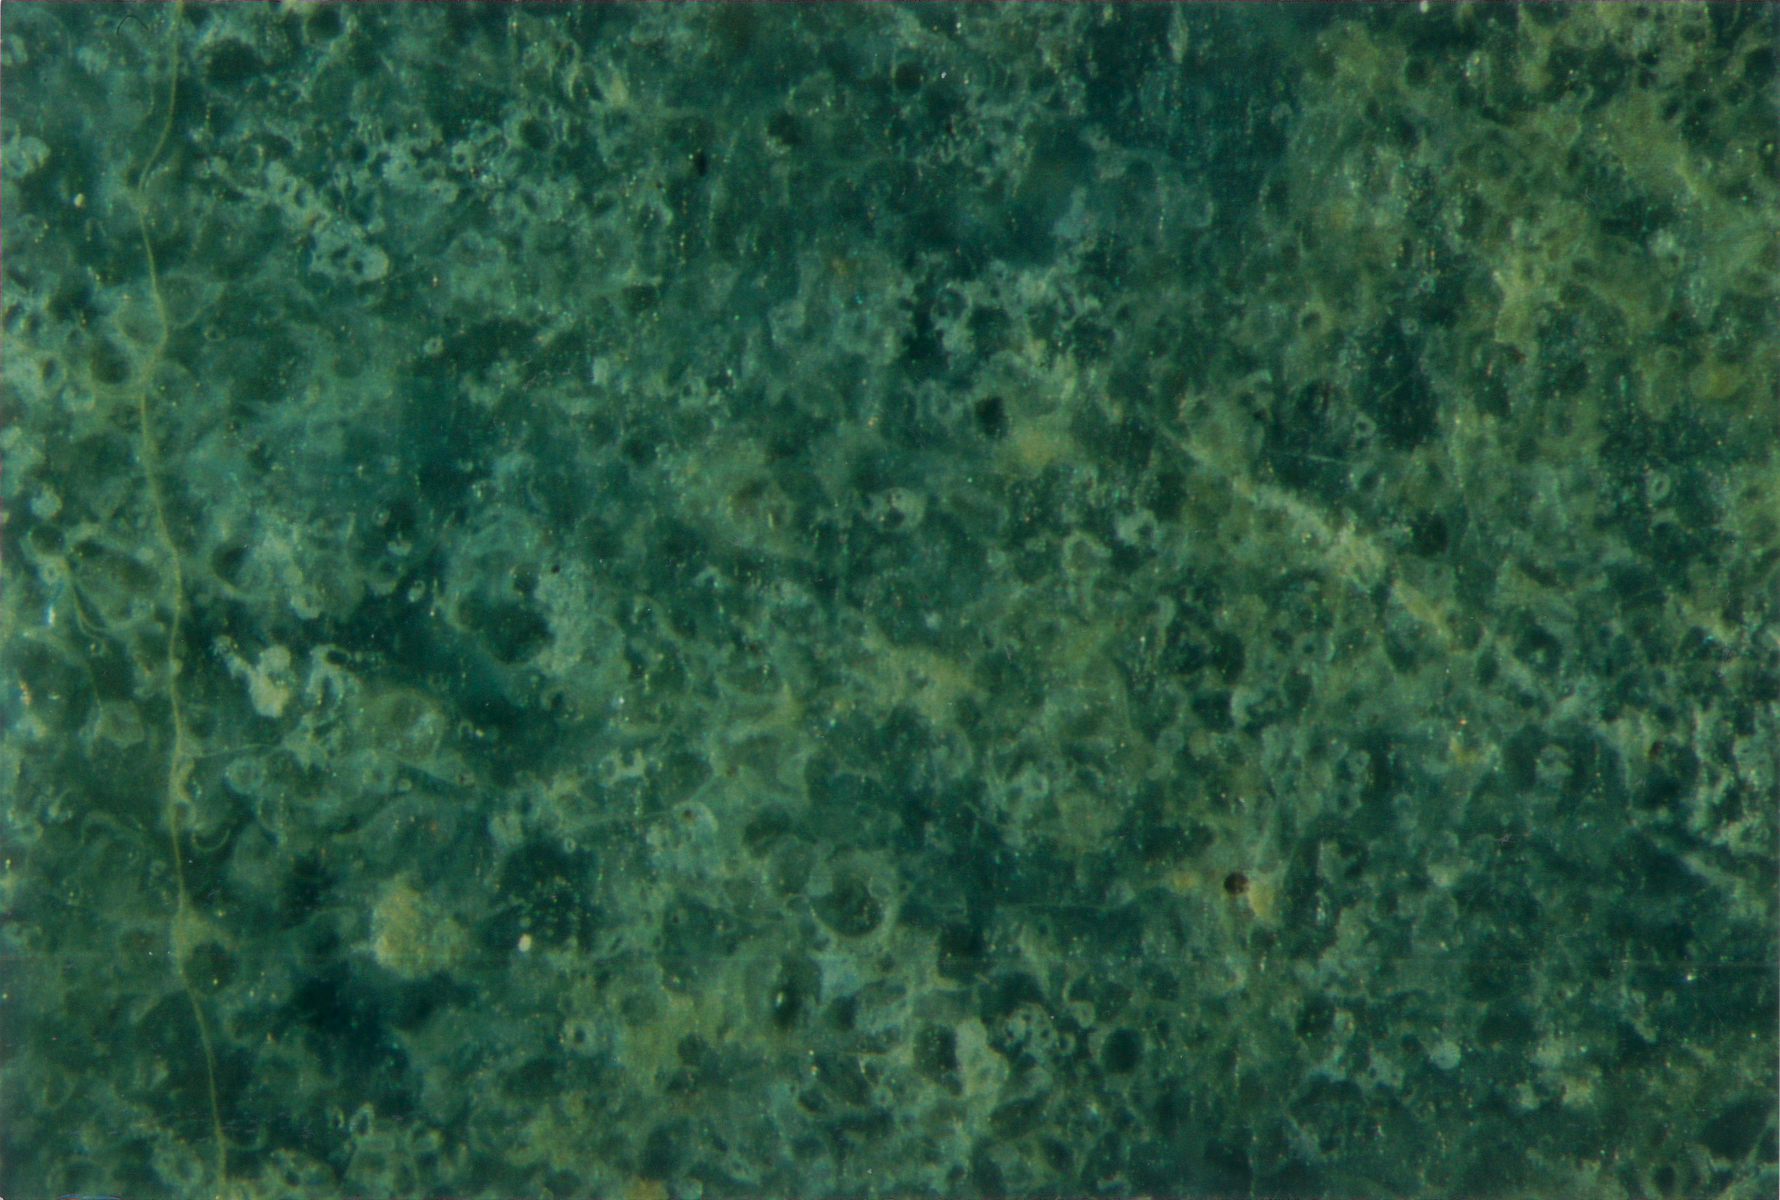
\includegraphics[width=\textwidth]{PaM_BDX6529_Surf}
  \caption[\bdx{6529}\ -- État de surface de la glaçure]
          {\legendeB.
           État de surface de la glaçure 
           (Gr=\num{30}, \zone{\sim4.3x3.2}{\mm}). 
           Elle contient des bulles et présente une forte usure 
           de surface.}
  \label{surf:6529}
\end{figure}


\section{Étude de la couleur}
%----------------------------------------------------------------------

\subsection{Identification des ions chromogènes}
%~~~~~~~~~~~~~~~~~~~~~~~~~~~~~~~~~~~~~~~~~~~~~~~~~~~~~~~~~~~~~~~~~~~~~~
Le spectre d'\AO en mode réflexion diffuse de la glaçure bleu vert 
(\fref{spectre:6529}) laisse apparaître trois bandes d'absorption à 
\SIlist{525;600;660}{\nm}, caractéristiques du \ch{Co^2+} 
\autocite{Lajarte_1979}.

\begin{figure}[htb]
  \begin{plotspectre}
    \addplot [thick, PowderBlue!75!black] 
       table [x=lambda, y=6529gla] {\gladata} ;
    \addlegendentry{glaçure bleue}
    \addplot [thick, PowderBlue!50!black] 
       table [x=lambda, y=6529glaSPMO] {\gladata} ;
    \addlegendentry{glaçure bleue, SPMO}
    \addplot [thick, FireBrick] 
       table [x=lambda, y=6529tc] {\tcdata} ;
    \addlegendentry{terre cuite}

    \begin{scope}[<-, >=stealth, shorten <=5pt, thin]
      \node (Co) at (595.00, 0.80) {\ch{Co^2+}} ;
      \draw (525.00, 0.56) |- (Co.south) ;
      \draw (600.00, 0.61) |- (Co.south) ;
      \draw (660.00, 0.59) |- (Co.south) ;
    \end{scope}
  \end{plotspectre}
  \caption[\bdx{6529}\ -- Spectres d'\AO en mode réflexion diffuse 
           de la glaçure et de la terre cuite]
          {\legendeB.
           Spectres d'\AO en mode réflexion diffuse de la glaçure et 
           de la terre cuite. La coloration de la glaçure est due au 
           \ch{Co^2+} mis en évidence par les trois bandes 
           d'absorption à \SIlist{525;600;660}{\nm}.}
  \label{spectre:6529}
\end{figure}

\subsection{Mesure physique de la couleur}
%~~~~~~~~~~~~~~~~~~~~~~~~~~~~~~~~~~~~~~~~~~~~~~~~~~~~~~~~~~~~~~~~~~~~~~
À partir du spectre d'\AO, ont été calculées les coordonnées 
chromatiques correspondant aux espaces \Yxy et \Lab 
(\tref{saotab:6529}). La longueur d'onde dominante associée 
au rayonnement correspond au domaine du vert jaunâtre 
\autocite{Kelly_1976}. Ce résultat, en contradiction avec 
l'observation visuelle, peut s'expliquer par la forte usure de la 
glaçure. En effet, elle laisse par endroit apparaître le support 
céramique rougeâtre sous-jacent, ce qui altère la perception de la 
couleur de la glaçure.

Nous avons donc utilisé un montage spectrophotomètre/microscope 
optique (Gr=40) permettent de focaliser le faisceau pour analyser 
une zone saine de la glaçure. Le spectre obtenu présente, lui aussi, 
les trois bandes d'absorption caractéristiques du \ch{Co^2+}. 
Les résultats de \CHRO sont consignés dans le \tref{saotab:6529} et 
la \fref{colorfig:6529} en donne les représentations graphiques. 
La longueur d'onde dominante est cette fois de \SI{482.54}{\nm}, 
elle correspond au domaine du bleu verdâtre \autocite{Kelly_1976}. 
La pureté d'excitation \SI{3.71}{\percent} est celle d'une couleur très 
peu saturée, la réflectance \CIEY (\num{27.839}) indique une couleur 
assez foncée.

\begin{table}[hbt]
  \caption[\bdx{6529}\ -- Coordonnées chromatiques et longueur d'onde 
           dominante]
          {\legendeB.
           Coordonnées chromatiques dans les systèmes \Yxy et \Lab 
           et longueur d'onde dominante (illuminant D65, \ang{2},
           \SIrange{400}{700}{\nm}). (\up{\dag}\,\cite{Kelly_1976})}
  \label{saotab:6529}
  \begin{chrotab}[Appareillage]
      \chrolgna{Spectro\-photo\-mètre}{551.45}{3.81}
               {27.953}{0.313}{0.343}
               {59.847}{-4.345}{3.382} &
      \chrolgnb{vert jaunâtre foncé}{Vert-Jaune}{530}{560}{}
    \tabularnewline
      \chrolgna{Spectro\-photo\-mètre + microscope optique}
               {482.54}{3.71}
               {27.839}{0.304}{0.323}
               {59.743}{-1.006}{-2.601} &
      \chrolgnb{bleu verdâtre foncé}{Bleu-verdâtre}{482}{487}{}
               % {\footnotemark{}}
    \tabularnewline
  \end{chrotab}
\end{table}
% \footnotetext{\autocite{Kelly_1976}}

\begin{figure}[htb]
  \newcommand{\samplename}{6529gla}
  \newcommand{\samplecolor}{PowderBlue}
  \begin{minipage}[t]{0.37\paperwidth}
    \begin{plotYxy}
      \plotYxyPaV ;
      \plotYxyIlluminant ;
      \plotYxySample{\samplename}{\samplecolor} ;
      \plotYxyLigne{\samplename} ;
      \plotYxyAnnot{\samplename}{north west} ;
    \end{plotYxy}
    \subcaption[Espace \trichro \Yxy]
               {Espace \trichro \Yxy. La longueur d'onde 
                dominante de la glaçure est de \SI{482.54}{\nm} et 
                correspond au domaine du bleu vert. La couleur est 
                très peu saturée : son point représentatif est très 
                proche de l'illuminant standard.}
  \end{minipage}%
  \qquad%
  \begin{minipage}[t]{0.37\paperwidth}
    \begin{plotLab}
      \plotLabSample{\samplename}{\samplecolor} ;
    \end{plotLab}
    \subcaption[Espace \trichro \Lab]
               {Espace \trichro \Lab. Le point représentatif de 
                la couleur de la glaçure est dans le quart vert-bleu.}
  \end{minipage}%
  \caption[\bdx{6529}\ -- Analyse chromamétrique de la glaçure]
          {\legendeB. Analyse chromamétrique de la glaçure.}
  \label{colorfig:6529}
\end{figure}


\section{Étude de la texture de la glaçure et de la terre cuite}
%----------------------------------------------------------------------

\subsection{Observation en lumière naturelle}
%~~~~~~~~~~~~~~~~~~~~~~~~~~~~~~~~~~~~~~~~~~~~~~~~~~~~~~~~~~~~~~~~~~~~~~
\begin{figure}[htb]
  \begin{minipage}[t]{0.48\textwidth}
    \fakeimg{lum. nat.}
    \subcaption{Lumière naturelle \label{texture:6529_LN}}
  \end{minipage}%
  \hfill%
  \begin{minipage}[t]{0.48\textwidth}
    \fakeimg{Cathodo}
    \subcaption{\CL \label{texture:6529_CL}}
  \end{minipage}
  \caption[\bdx{6529}\ -- Observation de la texture en section]
          {\legendeB.
           Observation de la texture en section 
           sur une surface de \SI{2.6x1.9}{\mm}.}
  \label{texture:6529}
\end{figure}

L'examen en section en lumière naturelle de l'ensemble terre 
cuite-glaçure (\fref{texture:6529_LN}), montre que la glaçure est 
colorée dans la masse et qu'elle adhère bien au support de terre cuite.

Cette dernière contient peu d'inclusions, blanches et rouges.

\subsection{Observation en \CL}
%~~~~~~~~~~~~~~~~~~~~~~~~~~~~~~~~~~~~~~~~~~~~~~~~~~~~~~~~~~~~~~~~~~~~~~
On peut distinguer dans l'ensemble de la glaçure 
(\fref{texture:6529_CL}), des cristaux présentant une 
luminescence mauve.

La terre cuite luminesce elle aussi en mauve. Elle contient quelques 
inclusions qui luminescent en rouge et en bleu.

Sur toute la largeur de la lame étudiée, on note la présence d'un 
large liseré luminescent en jaune à l'interface glaçure-terre cuite.


\subsection{Observation en \MEB[ie]}
%~~~~~~~~~~~~~~~~~~~~~~~~~~~~~~~~~~~~~~~~~~~~~~~~~~~~~~~~~~~~~~~~~~~~~~
La glaçure a une épaisseur moyenne de \SI{300}{\um}. Elle contient 
des bulles et de nombreux cristaux non fondus, dont la dimension peut 
aller jusqu'à \SI{100}{\um}. Elle semble avoir pénétré par endroits 
dans la terre cuite (\fref{MEB:6529_img}).

\begin{figure}[htb]
  \fakeimg{Texture au MEB, retrodiff (fig 33)}
  \caption[\bdx{6529}\ -- Observation de la texture au \MEB, 
           en mode \ERD. Ensemble glaçure/terre cuite]
          {\legendeB.
           Image en mode \ERD de l'ensemble glaçure/terre cuite. 
           La barre d'échelle mesure \SI{1}{\mm} (\zone{2.4x1.9}{\mm}).}
  \label{MEB:6529_img}
\end{figure}

Une \carto de \RX (\fref{MEB:6529_carto_tcgla}) a permis de montrer 
que ces cristaux sont des quartz (\quartz). Ils sont responsables 
des luminescences mauves détectées en \CL.

Des cristaux de forme aciculaire se développent à l'interface 
glaçure-terre cuite (\fref{MEB:6529_img_int}). Cette zone semble être 
riche en potassium, aluminium, calcium, mais plus pauvre en plomb que 
la glaçure environnante.

Le développement important de cette zone d'interface laisse supposer 
des interactions fortes entre glaçure et terre cuite, et donc, 
probablement, une application de la glaçure sur le support céramique 
avant cuisson de ce dernier.

\begin{figure}[htb]
  \fakeimg{Texture au MEB, retrodiff (fig 34)}
  \caption[\bdx{6529}\ -- Observation de la texture au \MEB, 
           en mode \ERD. Interface glaçure/terre cuite]
          {\legendeB
           Image en \ERD de l'interface glaçure/terre cuite. 
           La barre d'échelle mesure \SI{100}{\um} (\zone{370x300}{\um}).}
  \label{MEB:6529_img_int}
\end{figure}

Une \carto de la terre cuite (\fref{MEB:6529_carto_tc}) a permis de 
mettre en évidence la présence de cristaux de quartz et de feldspaths 
potassiques. Ces derniers sont à l'origine des luminescences 
ponctuelles bleues observées en \CL. Les luminescences rouges 
détectées en \CL peuvent être corrélées avec la présence dans la terre 
cuite de calcium, probablement sous forme de calcite (\calcite).

\begin{figure}[htb]
  \fakeimg{Texture au MEB, carto tc/gla (fig 35)}
  \caption[\bdx{6529}\ -- Observation de la texture au \MEB, \carto 
           de \RX de l'ensemble glaçure-terre cuite]
          {\legendeB.
           Observation de la texture au \MEB, \carto de \RX de 
           l'ensemble glaçure-terre cuite (Gr=90, \zone{1.2x1}{\mm}).}
  \label{MEB:6529_carto_tcgla}
\end{figure}

\begin{figure}[htb]
  \fakeimg{Texture au MEB, carto tc (fig 36)}
  \caption[\bdx{6529}\ -- Observation de la texture au \MEB, \carto 
           de \RX de la terre cuite]
          {\legendeB.
           Observation de la texture au \MEB, \carto de \RX de la 
           terre cuite (Gr=200, \zone{550x450}{\um}).}
  \label{MEB:6529_carto_tc}
\end{figure}


\section{Composition élémentaire de la glaçure}
%----------------------------------------------------------------------

\begin{table}[hbt]
  \caption[\bdx{6529}\ -- Analyse quantitative par \EDS, 
           composition élémentaire de la glaçure]
          {\legendeB. Analyse quantitative par \EDS. 
           Composition élémentaire de la glaçure bleue 
           sur une surface de \SI{54x44}{\um} (\PMO).}
  \label{compelem:6529_gla}
  \begin{cartotab}
      \cartolgn{SiO2}{34.02}{1.03} &
      \cartolgn{CaO}{1.95}{0.24} &
      \cartolgn{Al2O3}{0.35}{0.08} &
      \cartolgn{MgO}{0.39}{0.06} 
    \tabularnewline
      \cartolgn{Na2O}{0.50}{0.08} &
      \cartolgn{K2O}{1.56}{0.12} &
      \cartolgn{Fe2O3}{0.55}{0.13} &
      \cartolgn{PbO}{56.75}{1.46} 
    \tabularnewline
      \cartolgn{SnO2}{2.39}{0.24} &
      \cartolgnnd{CuO} &
      \cartolgnnd{CoO} &
      \cartolgnnd{MnO}
    \tabularnewline
      \cartolgnnd{Cr2O3} &
      \cartolgnnd{ZnO} &
      \cartolgnnd{Sb2O3} &
      \cartolgnnd{TiO2}
    \tabularnewline
      \cartolgn{S}{0.34}{0.05} &
      \cartolgn{P2O5}{0.70}{0.13} &
      \cartolgn{Cl}{0.51}{0.06} &
      \cartolgnnd{As2O3}
    \tabularnewline
  \end{cartotab}
\end{table}

La glaçure est plombifère et opacifiée à l'étain 
(\fref{compelem:6529_gla}). Le cobalt, responsable de la 
coloration bleue (mis en évidence par \SAO), n'est pas détecté. 
Il est probablement présent en concentration inférieure au seuil 
de détection de la méthode. Il possède en effet un très fort pouvoir 
colorant : \SI{0.25}{\percent} de cobalt suffisent à donner un bleu 
moyen \autocite{Rhodes_1999}.


\section{Étude de la terre cuite support}
%----------------------------------------------------------------------

\subsection{Composition élémentaire}
%~~~~~~~~~~~~~~~~~~~~~~~~~~~~~~~~~~~~~~~~~~~~~~~~~~~~~~~~~~~~~~~~~~~~~~
\begin{table}[hbt]
  \caption[\bdx{6529}\ -- Analyse quantitative par \EDS, 
           composition élémentaire de la terre cuite]
          {\legendeB. Analyse quantitative par \EDS. 
           Composition élémentaire de la terre cuite 
           sur une surface de \SI{1080x876}{\um} (\PMO)}
  \label{compelem:6529_tc}
  \begin{cartotab}
      \cartolgn{SiO2}{49.38}{0.61} &
      \cartolgn{CaO}{18.70}{0.88} &
      \cartolgn{Al2O3}{14.97}{0.33} &
      \cartolgn{MgO}{2.50}{0.35} 
    \tabularnewline
      \cartolgn{Na2O}{0.62}{0.07} &
      \cartolgn{K2O}{2.26}{0.21} &
      \cartolgn{Fe2O3}{9.06}{0.18} &
      \cartolgnnd{PbO}
    \tabularnewline
      \cartolgnnd{SnO2} &
      \cartolgnnd{CuO} &
      \cartolgnnd{CoO} &
      \cartolgnnd{MnO}
    \tabularnewline
      \cartolgnnd{Cr2O3} &
      \cartolgnnd{ZnO} &
      \cartolgnnd{Sb2O3} &
      \cartolgn{TiO2}{0.85}{0.03}
    \tabularnewline
      \cartolgnnd{S} &
      \cartolgn{P2O5}{1.59}{0.15} &
      \cartolgn{Cl}{0.07}{0.01} &
      \cartolgnnd{As2O3}
    \tabularnewline
  \end{cartotab}
\end{table}

La terre cuite est de type calcique (\SI{18.70}{\percent} de CaO). 
Sa coloration ocre rose est due au \ch{Fe^3+} en atmosphère de cuisson 
oxydante \autocite{Echallier_1984}.

\subsection{Composition \cristallo}
%~~~~~~~~~~~~~~~~~~~~~~~~~~~~~~~~~~~~~~~~~~~~~~~~~~~~~~~~~~~~~~~~~~~~~~
Le principal composé cristallisé mis en évidence par \DX sur poudre 
(\fref{DRX:6529}) est le quartz (\quartz). On relève également la 
présence, à des teneurs plus faibles, de calcite (\calcite) pouvant 
correspondre aux émissions rouges détectées en \CL, d'albite (\albite), 
de diopside alumineux (\diopsideal) et de gehlénite (\gehlenite). 
Ces deux derniers cristaux peuvent être responsables des émissions 
bleues détectées en \CL.

La présence de diopside alumineux et de gehlénite, deux phases se 
développant à haute température, associées à l'albite, disparaissant 
vers \SI{900}{\degC} au profit de l'anorthite, laisse penser que la 
température de cuisson de la céramique se situe autour de 
\SIrange{850}{900}{\degC} \autocite{Peters_1978}.

\begin{figure}[htb]
  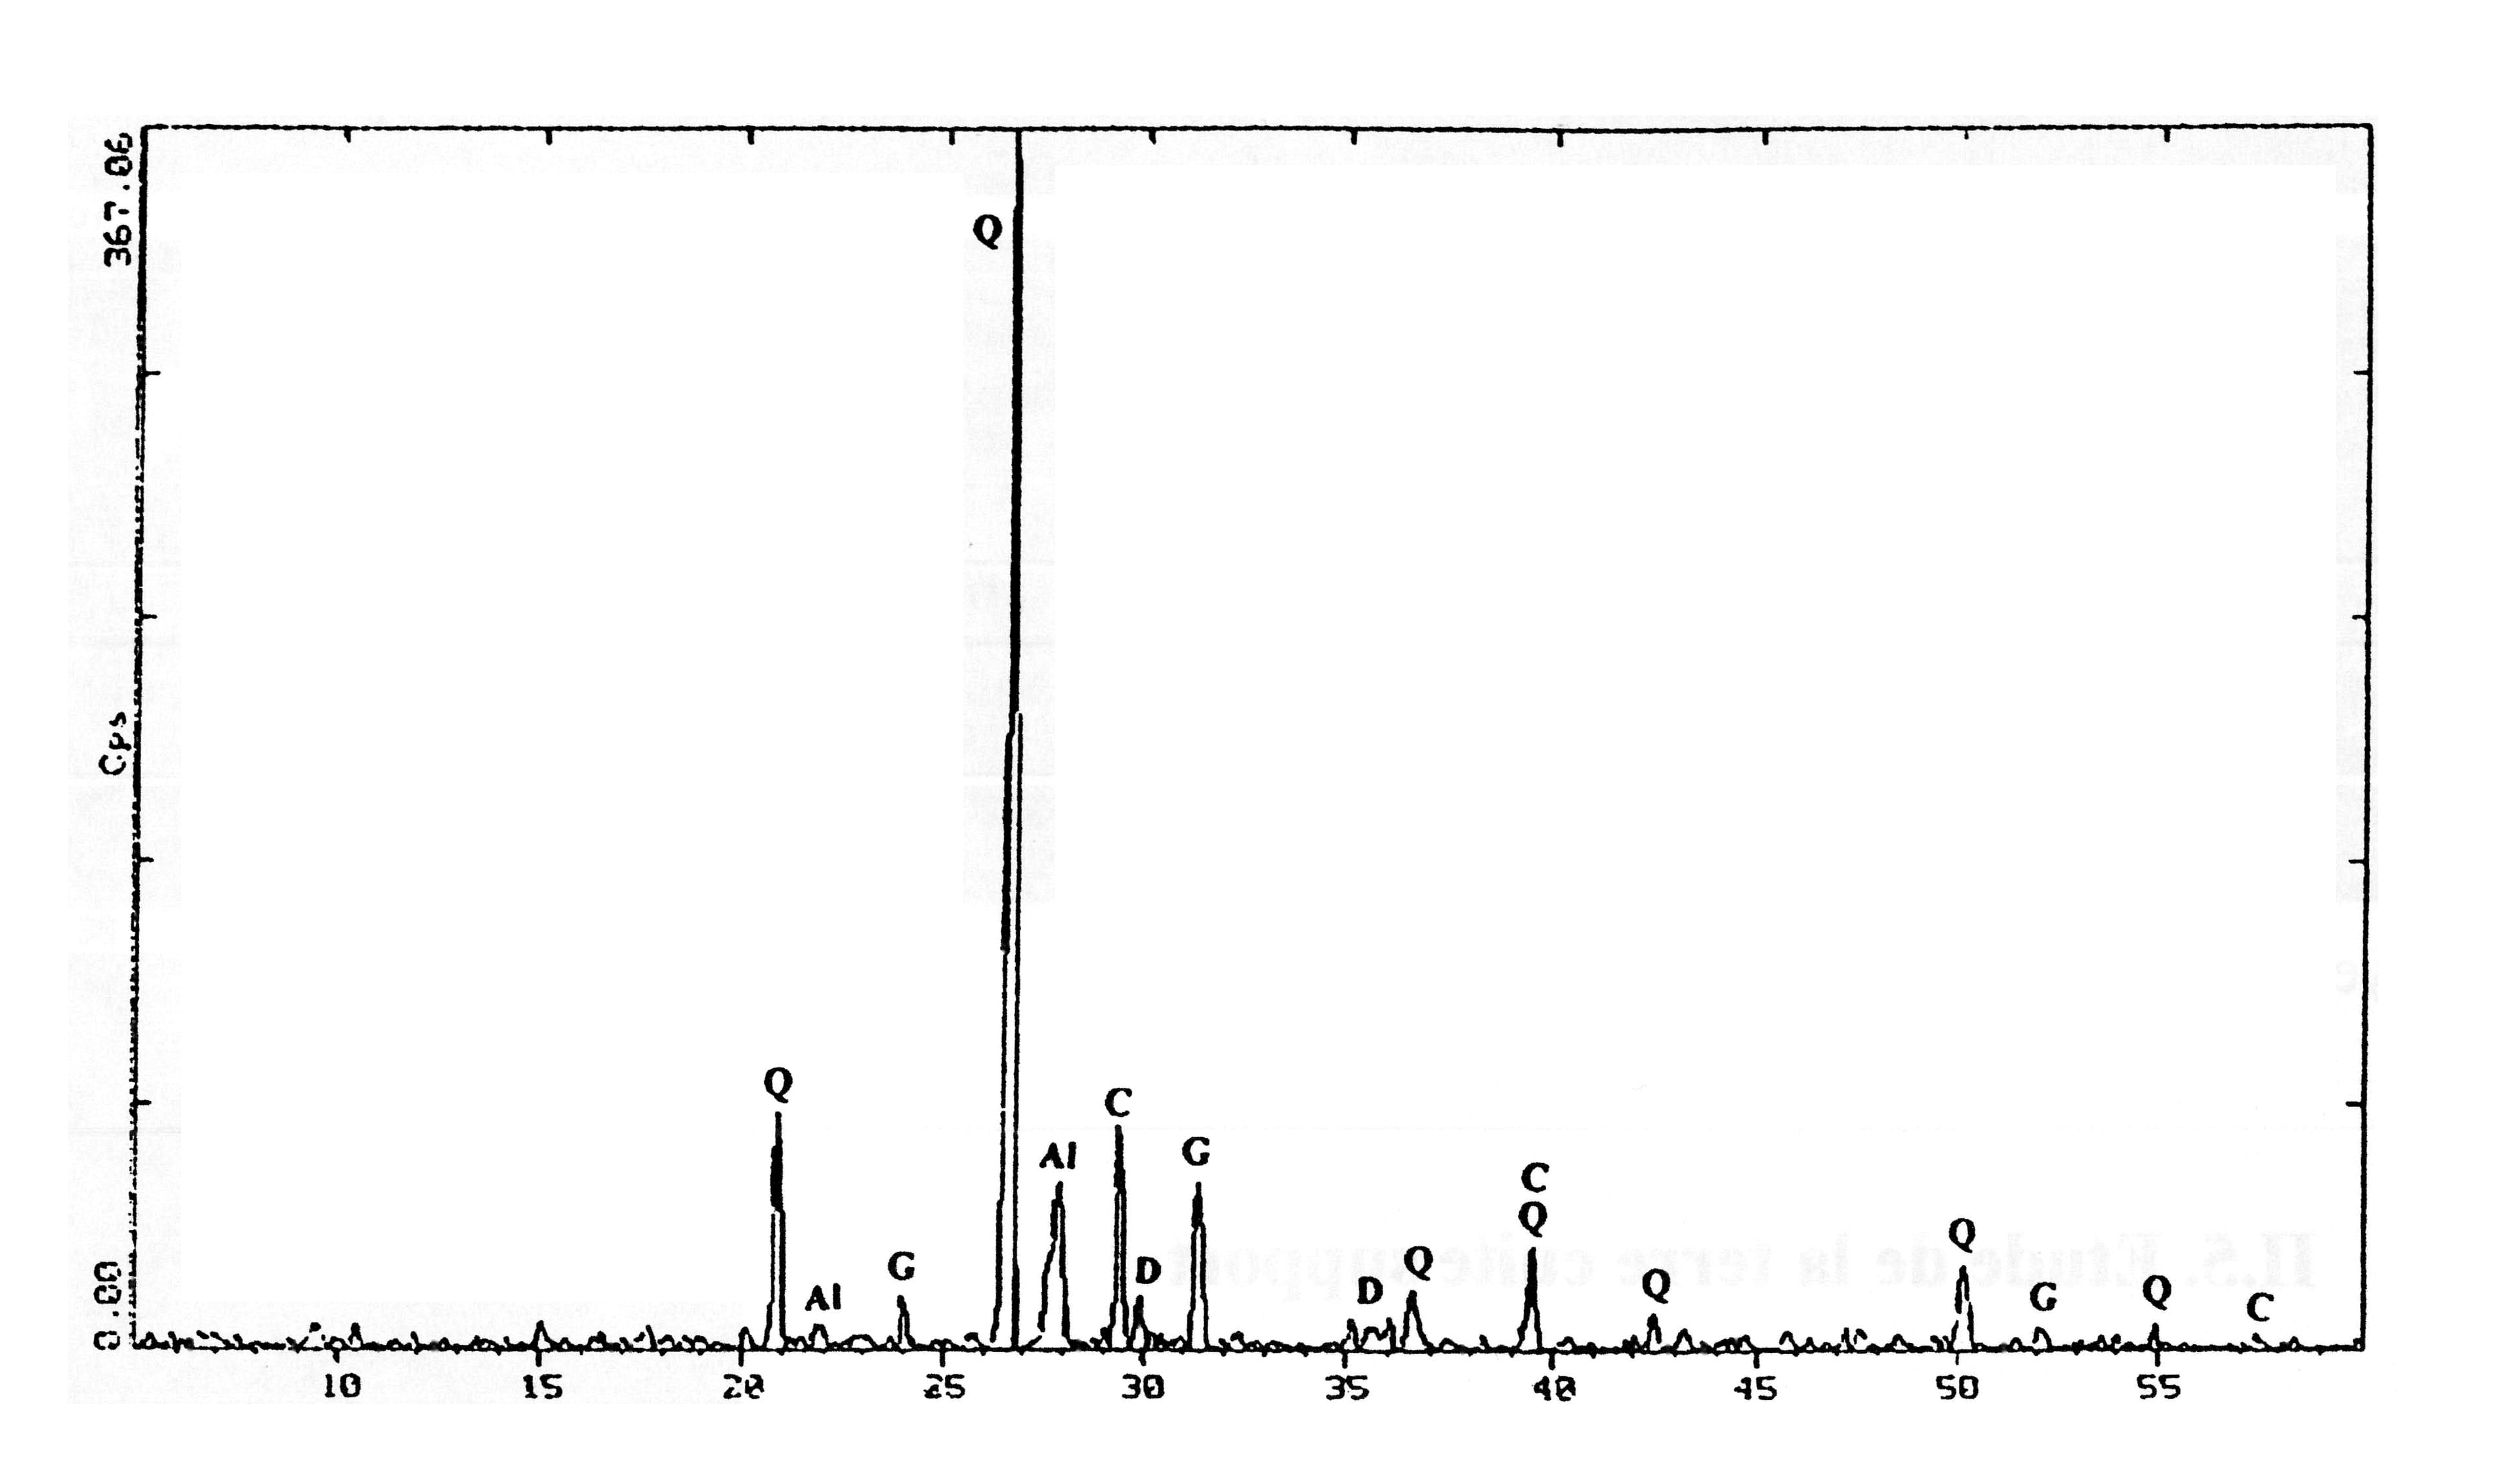
\includegraphics[width=\textwidth]{PaM_BDX6529_DX}
  \caption[\bdx{6529}\ -- Diffraction de \RX sur poudre 
           de la terre cuite]
          {\legendeB.
           \DX[D] sur poudre de la terre cuite. 
           Mise en évidence de la présence de quartz (Q), 
           calcite (C), albite (Al), gehlénite (G), diopside (D).}
  \label{DRX:6529}
\end{figure}


\section{Sur la présence et l'identification de cristaux de 
         dévitrification}
%----------------------------------------------------------------------

On distingue, dans la zone d'interface terre cuite-glaçure, des 
cristaux de forme aciculaire (\fref{MEB:6529_img_cx}). Ce sont 
des cristaux de dévitrification qui se développent pendant le 
refroidissement lent du matériau, à partir de germes se formant à 
haute température. Des analyses ponctuelles (\tref{compelem:6529_cx}) 
ont montré qu'il s'agit d'alumino-silicates mixtes de potassium, de 
calcium et de plomb que l'on peut appeler des \frquote{feldspaths de 
plomb}.


\begin{figure}[htb]
  \fakeimg{MEB img cx (fig 38)}
  \caption[\bdx{6529}\ -- Image en mode \ERD, 
           cristaux de dévitrification de forme aciculaire]
          {\legendeB.
           Observation au \MEB, image en mode \ERD. 
           Cristaux de dévitrification de forme aciculaire. La barre 
           d'échelle mesure \SI{20}{\um} (\zone{70x55}{\um}).}
  \label{MEB:6529_img_cx}
\end{figure}


\begin{table}[hbt]
  \caption[\bdx{6529}\ -- Analyse quantitative par \EDS, 
           composition élémentaire des cristaux de dévitrification]
          {\legendeB. Analyse quantitative par \EDS. 
           Composition élémentaire des cristaux de dévitrification 
           par analyses ponctuelles (\SI{1}{\um\squared}) (\PMO).}
  \label{compelem:6529_cx}
  \begin{cartotab}
      \cartolgn{SiO2}{54.61}{6.48}  &
      \cartolgn{CaO}{3.51}{1.64}    &
      \cartolgn{Al2O3}{11.80}{2.82} &
      \cartolgn{MgO}{0.28}{0.13}
    \tabularnewline
      \cartolgn{Na2O}{1.06}{0.13}  &
      \cartolgn{K2O}{9.44}{2.19}   &
      \cartolgn{Fe2O3}{2.09}{0.32} &
      \cartolgn{PbO}{16.83}{10.17}
    \tabularnewline
      \cartolgnnd{SnO2} &
      \cartolgnnd{CuO}  &
      \cartolgnnd{CoO}  &
      \cartolgnnd{MnO}
    \tabularnewline
      \cartolgnnd{Cr2O3} &
      \cartolgnnd{ZnO}   &
      \cartolgnnd{Sb2O3} &
      \cartolgn{TiO2}{0.14}{0.09}
    \tabularnewline
      \cartolgnnd{S}            &
      \cartolgnnd{P2O5}         &
      \cartolgn{Cl}{0.24}{0.15} &
      \cartolgnnd{As2O3}
    \tabularnewline
  \end{cartotab}
\end{table}


\section{Étude des altérations de la glaçure}
%----------------------------------------------------------------------

Aucune figure d'altération n'a été mise en évidence dans la glaçure, 
ni visuellement, ni en \MEB[ie] (MEB).


\section{Bilan}
%----------------------------------------------------------------------

Cet échantillon est donc une pièce de céramique portant une glaçure 
plombifère dont la coloration bleue est due au \ch{Co^2+} en 
atmosphère de cuisson oxydante et légèrement opacifiée à l'étain pour 
rendre la couleur plus veloutée et masquer la terre cuite rougeâtre.

Son support de terre cuite est de type calcique. Sa coloration 
rougeâtre est due à la présence de \ch{Fe^3+} en atmosphère de 
cuisson oxydante.

Sa composition \cristallo (quartz, calcite, albite, diopside, 
gehlénite) laisse penser qu'elle a été cuite à une température 
de l'ordre de \SIrange[range-phrase=\ à\ ]{850}{900}{\degC}.

À l'interface glaçure-terre cuite, on distingue un large liseré 
continu présentant une luminescence jaune, associé à la présence de 
cristaux de dévitrification identifiés comme des alumino-silicates 
mixtes de potassium, de calcium et de plomb (ou \frquote{feldspaths 
de plomb}). Le développement important de cette zone laisse penser à
une application de la glaçure sur la terre crue.

La glaçure ne présente pas de figure d'altération d'origine chimique 
mais une usure mécanique de surface.

%!TEX root = MemoireZelliges.tex

\chapter{Étude physique d'un zellige noir (\bdx{6530})}
%======================================================================

\section{Description -- État de surface}
%----------------------------------------------------------------------

Cet échantillon, de forme parallélépipédique (\fref{dessin:6530}), est 
une pièce de céramique glaçurée de couleur  noire. Il provient du \PaM 
(\siecle{17}) de Meknès.

\begin{itemize}
  \item \DimText : \SI{30x30x21}{\mm}
  \item \emph{Masse} : \SI{20.0}{\g}
\end{itemize}

\begin{figure}[htb]
  \begin{minipage}[t]{0.5\textwidth}
    \centerfloat
    \vspace*{0pt}
    % Dessin de l'échantillon : Vue de dessus
    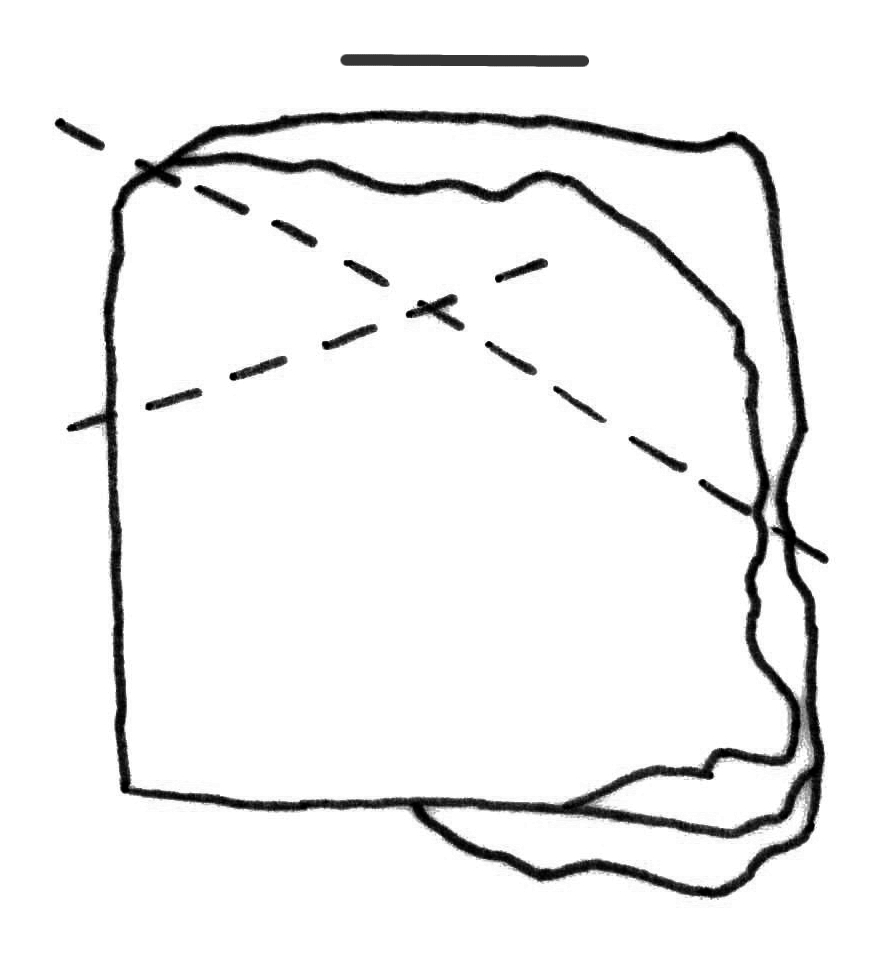
\includegraphics[scale=1]{PaM_BDX6530_dessus}
    \subcaption{Vue de dessus \label{dessin:6530_dessus}}
  \end{minipage}%
  \quad%
  \begin{minipage}[t]{0.5\textwidth}
    \centerfloat
    \vspace*{0pt}
    % Dessin de l'échantillon : Lame
    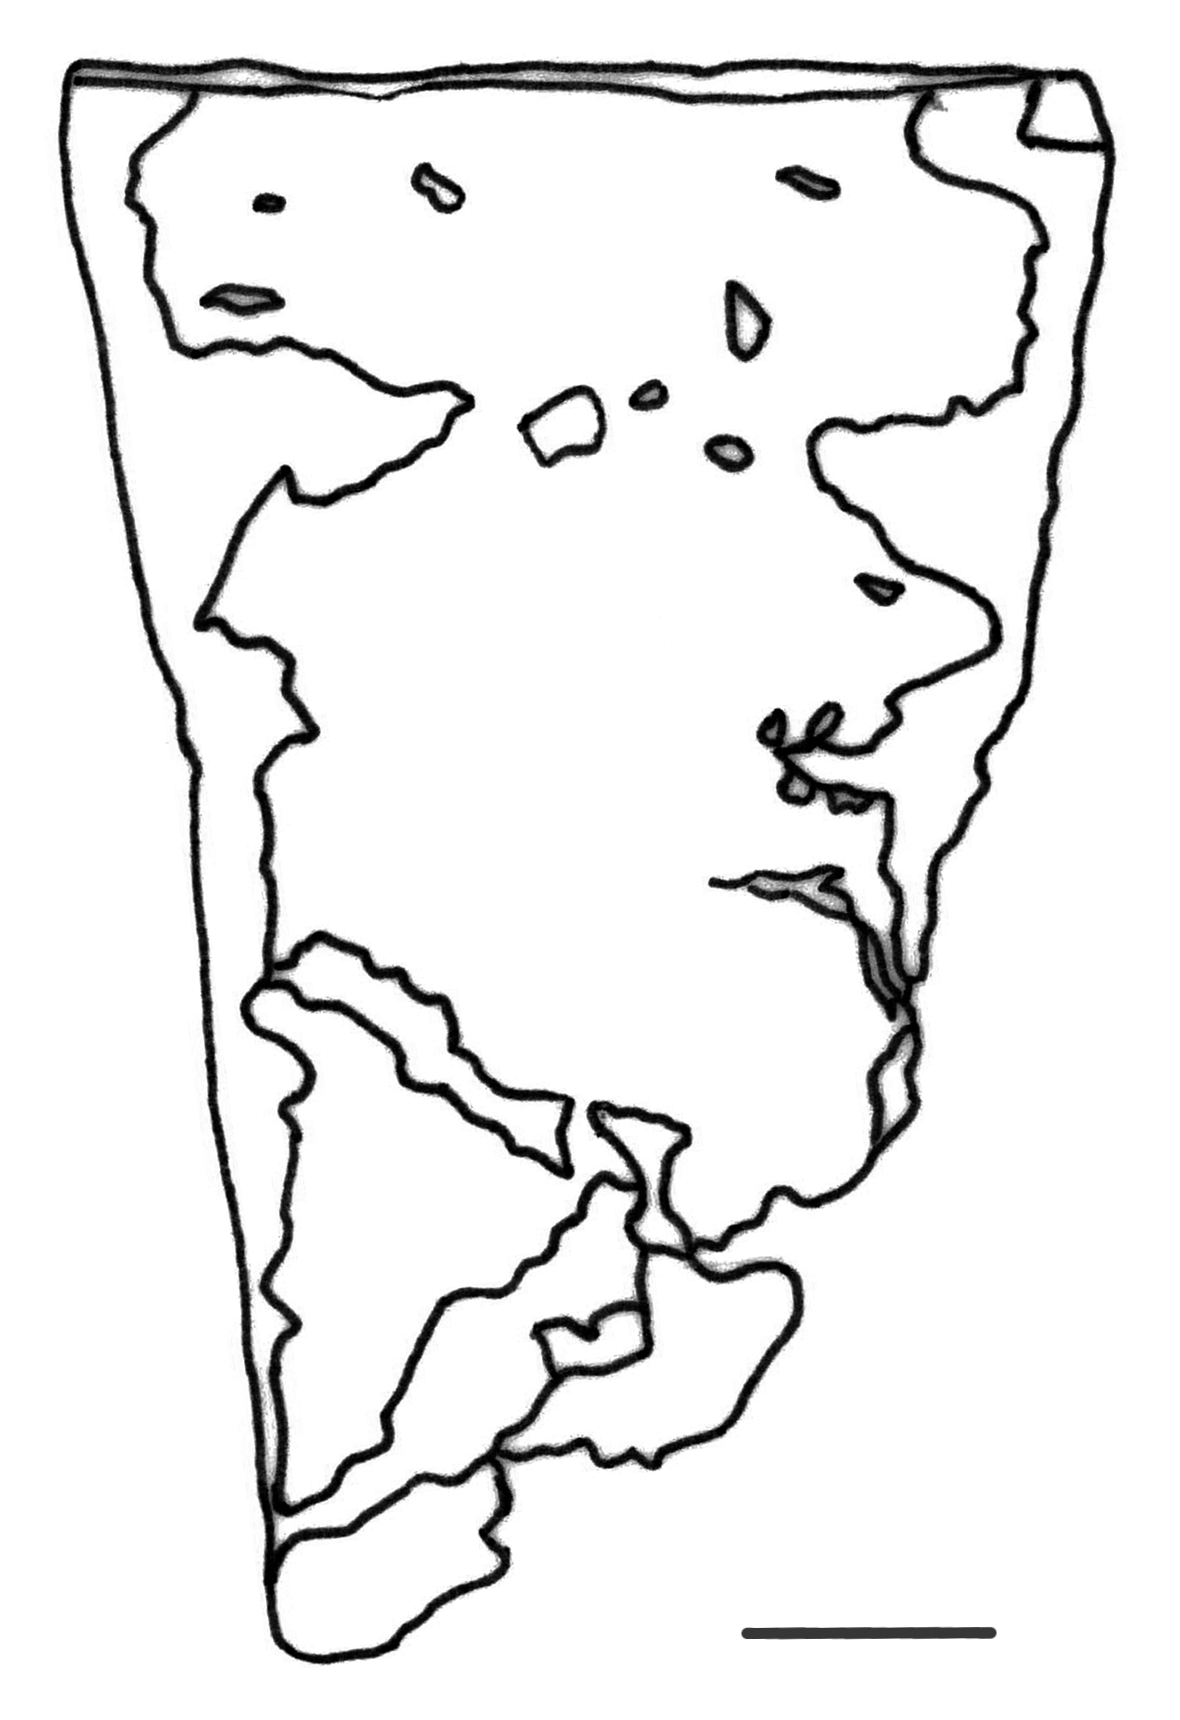
\includegraphics[scale=1]{PaM_BDX6530_lame}
    \subcaption{Lame étudiée \label{dessin:6530_lame}}
  \end{minipage}

  \bigskip

  \begin{minipage}[t]{0.5\textwidth}
    \centerfloat
    \vspace*{0pt}
    % Dessin de l'échantillon : Coupe
    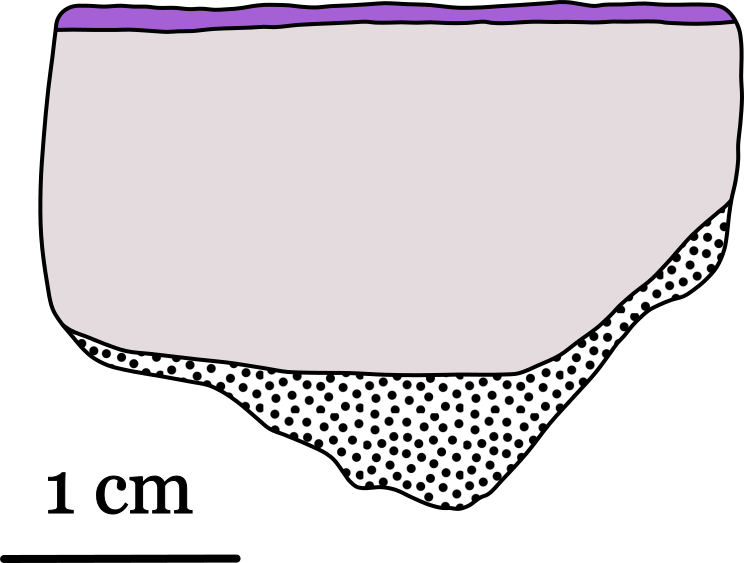
\includegraphics[scale=1]{PaM_BDX6530_coupe}
    \subcaption{Vue en coupe \label{dessin:6530_coupe}}
  \end{minipage}%
  \quad%
  \begin{minipage}[t]{0.5\textwidth}
    \vspace*{0pt}
    Légende :

    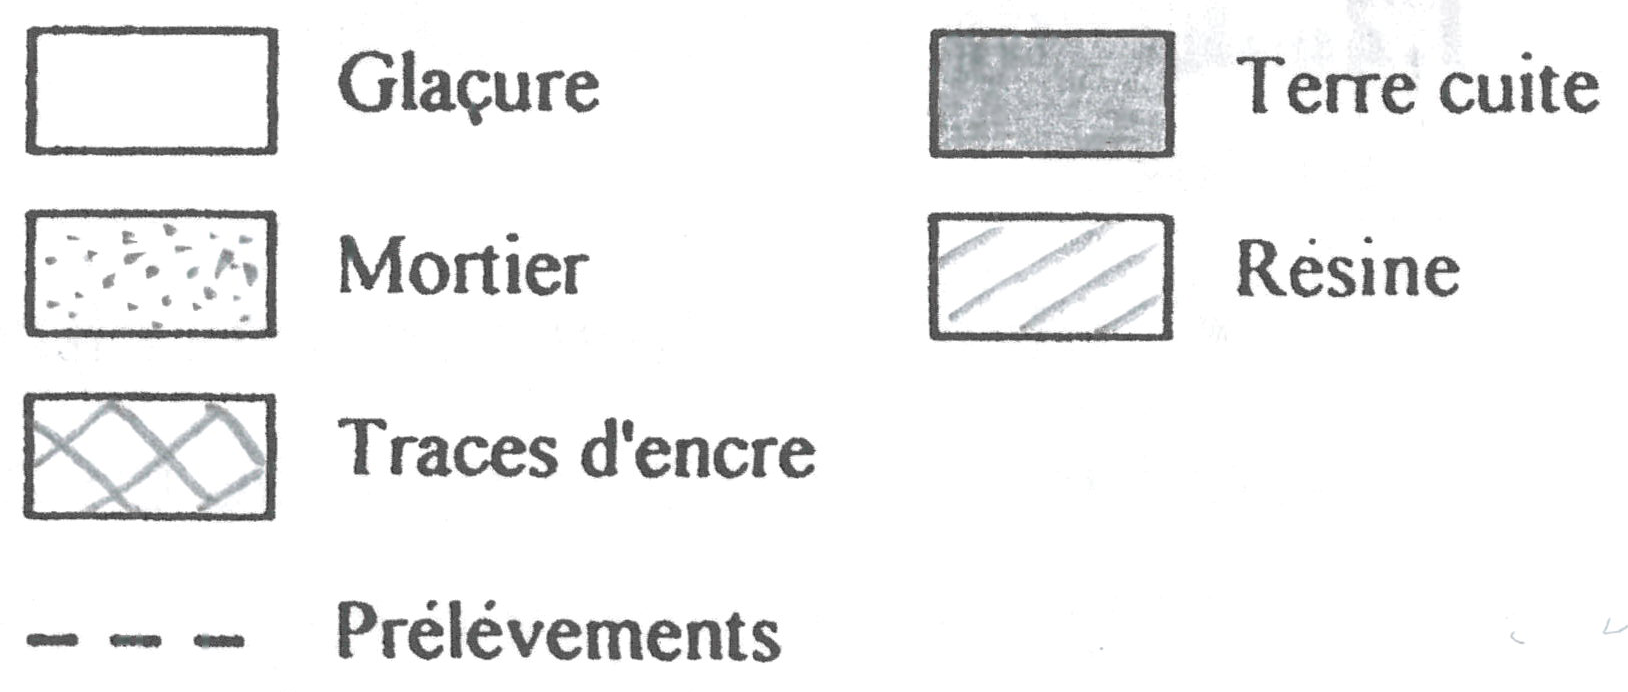
\includegraphics[scale=1]{dessin_legende}
    % \begin{itemize}
    %   \item Terre cuite
    %   \item Glaçure
    %   \item Résine
    %   \item Mortier
    %   \item Traces d'encre
    %   \item Prélévements
    % \end{itemize}
  \end{minipage}
  \caption{\legendeB 
           a : vue de dessus, b : vue en coupe, c : lame étudiée.}
  \label{dessin:6530}
\end{figure}

L'observation de la surface de la glaçure (\fref{surf:6530}) montre 
qu'elle contient des bulles, des picots, présente des rayures. On peut 
aussi y remarquer des petits cristaux en forme de baguettes.

Le support de terre cuite est de couleur rosé, de granulométrie fine, 
peu poreux et contient de nombreuses inclusions de tailles et de 
couleurs variées.

\begin{figure}[htb]
  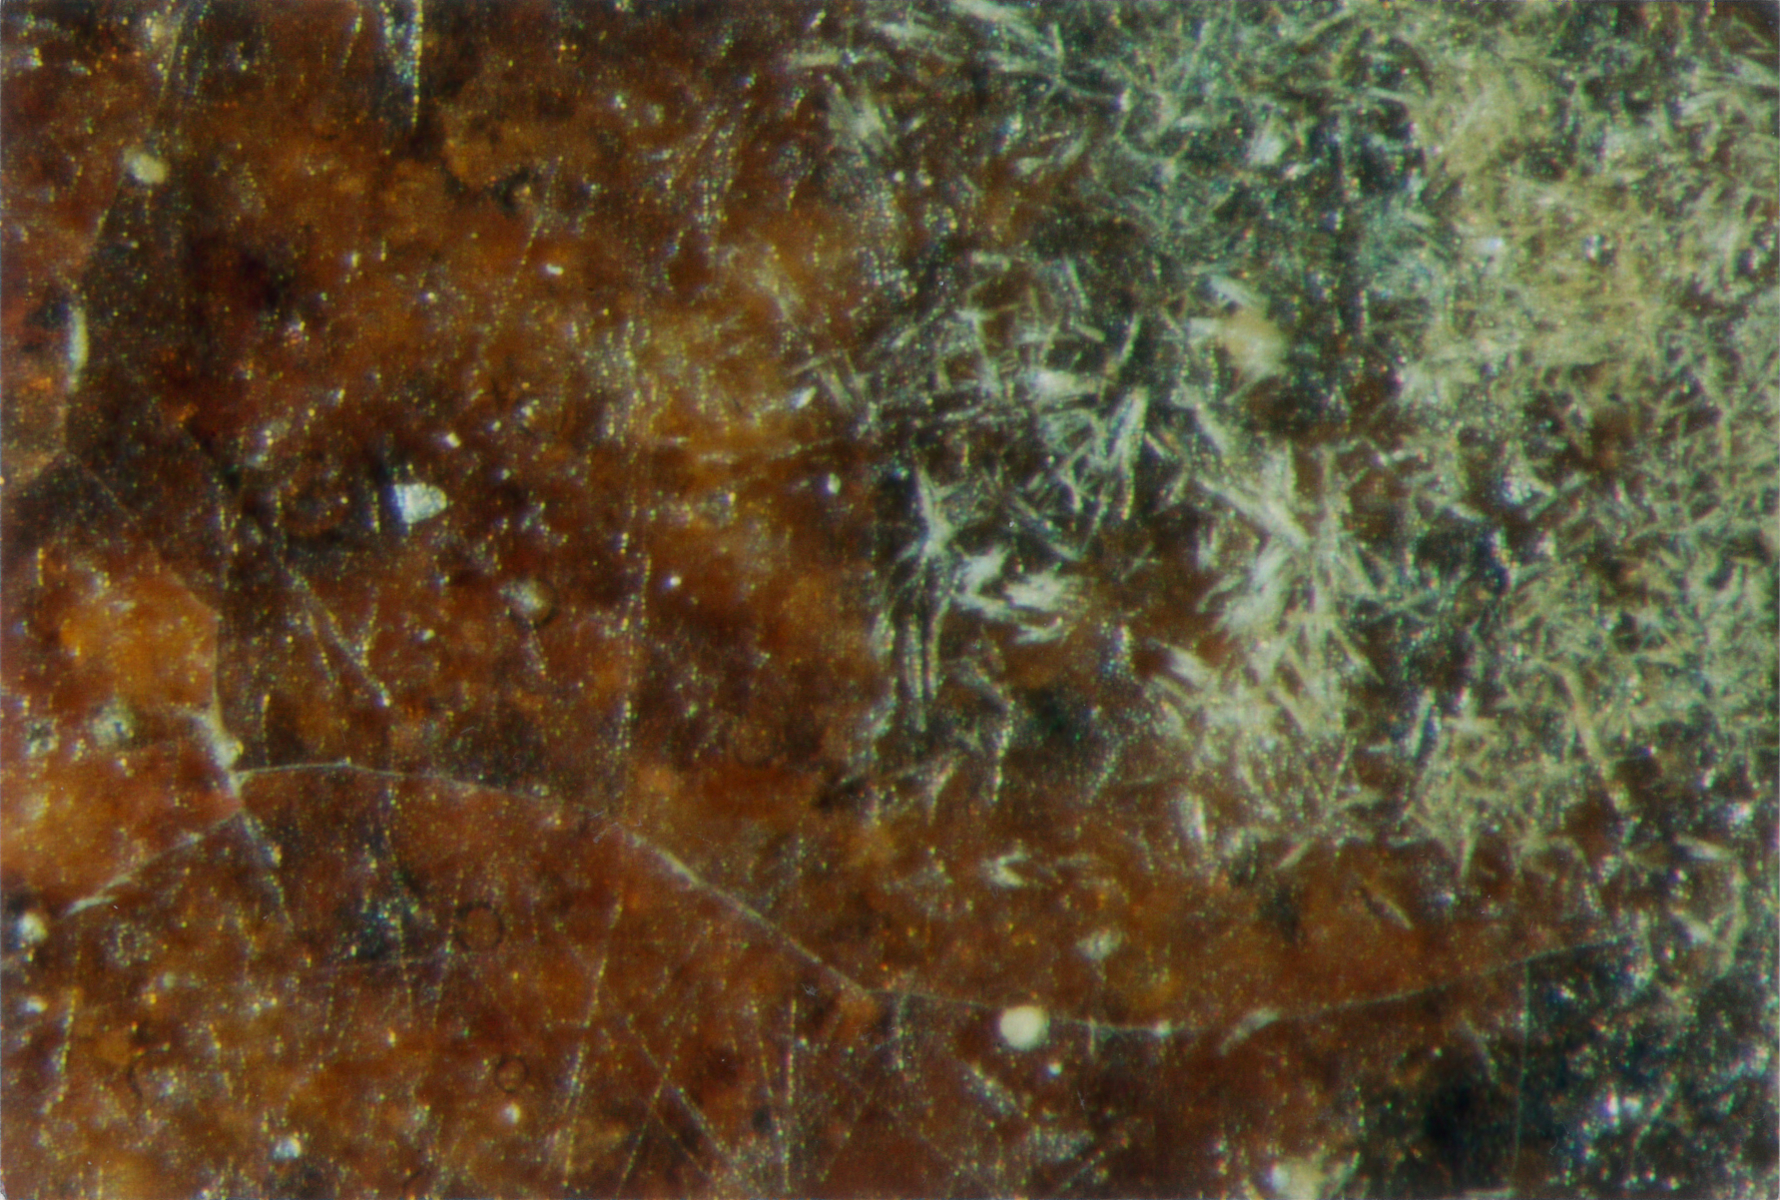
\includegraphics[width=\textwidth]{PaM_BDX6530_Surf}
  \caption{\legendeC 
           État de surface de la glaçure (Gr=\num{40}, \zone{\sim3.3x2.4}{\mm}). Elle contient des 
           bulles, des picots et présente des rayures.}
  \label{surf:6530}
\end{figure}


\section{Étude de la couleur}
%----------------------------------------------------------------------

\subsection{Identification des ions chromogènes}
%~~~~~~~~~~~~~~~~~~~~~~~~~~~~~~~~~~~~~~~~~~~~~~~~~~~~~~~~~~~~~~~~~~~~~~
\begin{figure}[htb]
  \begin{plotspectre}
    \addplot [thick, Indigo] 
       table [x=lambda, y=6530gla] {\gladata} ;
    \addplot [thick, FireBrick] 
       table [x=lambda, y=6530tc] {\tcdata} ;
  \end{plotspectre}
  \caption{\legendeC 
           Spectres d'\AO en mode réflexion diffuse de la glaçure et de la terre cuite. Le spectre présente une forte absorption dans tout le domaine visible (\SIrange{400}{700}{\nm}). Il se compose en fait d'une superposition de bandes d'absorption.}
  \label{spectre:6530}
\end{figure}

Le spectre d'\AO en mode réflexion diffuse de la glaçure (\fref{spectre:6530}) présente une forte absorption dans l'ensemble du domaine du visible avec toutefois une transmission un peu plus élevée à partir de \SI{550}{\nm}.

On ne distingue pas de bande d'absorption particulière. Le spectre est 
en fait constitué d'une superposition de bandes d'absorption plus ou 
mois larges et plus ou moins intenses.

La glaçure étant transparente, nous avons également enregistré le spectre d'\AO de la terre cuite support. Celui-ci présente une bande d'absorption à \SI{440}{\nm} qui correspond au \ce{Fe^3+} \autocite{Lajarte_1979}. La bande à \SI{550}{\nm} n'a pu être attribuée.

\subsection{Mesure physique de la couleur}
%~~~~~~~~~~~~~~~~~~~~~~~~~~~~~~~~~~~~~~~~~~~~~~~~~~~~~~~~~~~~~~~~~~~~~~
\begin{table}
  \begin{chrotab}
      \chrolgna{Glaçure}{594.39}{8.88}
               {6.505}{0.338}{0.335}
               {30.652}{4.036}{2.934} &
      \chrolgnb{orange très foncé}{Orange}{585}{600}
               {\footcite{Kelly_1976}}
    \tabularnewline
      \chrolgna{Terre cuite}{579.70}{23.30}
               {47.348}{0.359}{0.366}
               {74.412}{3.957}{18.143} &
      \chrolgnb{jaune orange clair}{Jaune-Orange}{580}{585}
               {\footcite{Kelly_1976}}
    \tabularnewline
  \end{chrotab}
  \caption{\legendeC 
           Coordonnées chromatiques dans les systèmes \Yxy et \Lab 
           et longueur d'onde dominante (illuminant D65, \ang{2},
           \SIrange{400}{700}{\nm}).}
  \label{saotab:6530}
  \footnotetext{\autocite{Kelly_1976}}
\end{table}

\begin{figure}[htb]
  \newcommand{\samplename}{6530gla}
  \newcommand{\samplecolor}{Indigo}
  \begin{minipage}[t]{0.37\paperwidth}
    \begin{plotYxy}
      \plotYxyPaV ;
      \plotYxyIlluminant ;
      \plotYxySample{\samplename}{\samplecolor} ;
      \plotYxyLigne{\samplename} ;
      \plotYxyAnnot{\samplename}{south west} ;
    \end{plotYxy}
    \subcaption{espace \trichro \Yxy. La longueur d'onde 
                dominante de la glaçure est de \SI{594.380}{\nm} 
                et correspond au domaine du orange.}
  \end{minipage}%
  \qquad%
  \begin{minipage}[t]{0.37\paperwidth}
    \begin{plotLab}
      \plotLabSample{\samplename}{\samplecolor} ;
    \end{plotLab}
    \subcaption{espace \trichro \Lab.}
  \end{minipage}%
  \caption[\bdx{6530}\ -- Espaces \trichros]
          {\legendeC Analyse chromamétrique de la glaçure.}
  \label{colorfig:6530}
\end{figure}

Les spectres d'\AO de la glaçure et de la terre cuite ont permis de calculer les coordonnées chromatiques correspondant aux espaces \Yxy et \Lab. La longueur d'onde dominante de la glaçure est de \SI{594.39}{\nm} (\tref{saotab:6530}), elle appartient au domaine des orange. La pureté d'excitation indique une couleur très peu saturée et la réflectance $Y$ est celle d'une couleur très foncée. Ce que l'on prend au premier abord pour un noir est en fait un orange très foncé, un noir. La longueur d'onde dominante de la terre cuite (\SI{579.70}{\nm}) se place dans le domaine du jaune-orange. Sa réflectance est assez élevée, la couleur est donc assez claire. La \fref{colorfig:6530} montre la localisation des cordonnées chromatiques de la glaçure noire dans les espaces \Yxy et \Lab.


\section{Étude de la texture de la glaçure et de la terre cuite}
%----------------------------------------------------------------------

\subsection{Observation en lumière naturelle}
%~~~~~~~~~~~~~~~~~~~~~~~~~~~~~~~~~~~~~~~~~~~~~~~~~~~~~~~~~~~~~~~~~~~~~~
\begin{figure}[htb]
  \begin{minipage}[t]{0.4\textwidth}
    \fakeimg{lum. nat.}
    \subcaption{Lumière naturelle \label{texture:6530_LN}}
  \end{minipage}
  \begin{minipage}[t]{0.4\textwidth}
    \fakeimg{Cathodo}
    \subcaption{\CL \label{texture:6530_CL}}
  \end{minipage}
  \caption[\bdx{6530}\ -- Observation de la texture en section]
          {\legendeC 
           Observation de la texture en section sur une surface de 
           \SI{2.6x1.9}{\mm}.}
  \label{texture:6530}
\end{figure}

L'examen en section en lumière naturelle de l'ensemble terre 
cuite/glaçure (\fref{texture:6530_LN}), montre que la glaçure est 
colorée dans la masse et qu'elle adhère bien au support de terre cuite.

Cette dernière contient diverses inclusions de faibles dimensions,
noires, rouges, blanches.

\subsection{Observation en \CL}
%~~~~~~~~~~~~~~~~~~~~~~~~~~~~~~~~~~~~~~~~~~~~~~~~~~~~~~~~~~~~~~~~~~~~~~
La glaçure n'est pas luminescente (\fref{texture:6530_CL}).

La terre cuite présente une luminescence mauve sur laquelle se 
détachent des luminescences ponctuelles rouges et bleues.

On n'observe aucune luminescence à l'interface glaçure/terre cuite.

Les quelques points jaunes que l'on peut remarquer dans la terre cuite 
et à la surface de la glaçure sont des résidus de la suspension 
diamantée utilisée pour le polissage de la lame.

\subsection{Observation en \MEB[ie]}
%~~~~~~~~~~~~~~~~~~~~~~~~~~~~~~~~~~~~~~~~~~~~~~~~~~~~~~~~~~~~~~~~~~~~~~
La glaçure a une épaisseur moyenne de \SI{170}{\um} et contient 
des bulles (\fref{MEB:6530_img}). On distingue des cristaux de 
forme aciculaire dans sa masse et d'autres cristaux à l'interface 
glaçure/terre cuite.

\begin{figure}[htb]
  \fakeimg{Texture au MEB, retrodiff (fig 44)}
  \caption[\bdx{6530}\ -- Observation de la texture au \MEB, 
           en mode \ERD. Ensemble glaçure/terre cuite]
          {\legendeC
           Observation de la texture au \MEB, en mode \ERD. 
           Ensemble glaçure/terre cuite. La barre d'échelle mesure 
           \SI{200}{\um} (\zone{550x440}{\um}).}
  \label{MEB:6530_img}
\end{figure}

Une \carto de \RX de l'ensemble terre cuite/glaçure (\fref{MEB:6530_carto_tcgla}) met en évidence la présence de manganèse et de plomb dans la glaçure. Elle est en revanche plus pauvre en calcium, aluminium et potassium que la terre cuite. Les cristaux de forme aciculaires se développant dans la masse de la glaçure semblent riches en calcium et manganèse mais dépourvus de plomb.

\begin{figure}[htb]
  \fakeimg{Texture au MEB, carto tc/gla (fig 45)}
  \caption[\bdx{6530}\ -- Observation de la texture au \MEB, \carto de \RX de l'ensemble glaçure/terre cuite]
          {\legendeC
           Observation de la texture au \MEB, \carto de \RX de l'ensemble glaçure/terre cuite (Gr=200, \zone{550x440}{\um}).}
  \label{MEB:6530_carto_tcgla}
\end{figure}

L'interface terre cuite/glaçure présente une forte concentration en 
potassium. Son faible développement semble indiquer des interactions 
faibles entre ces deux matériaux et l'on peut donc envisager 
l'hypothèse de l'application du mélange glaçurant sur une terre crue.

La terre cuite contient des inclusions identifiées par \carto de \RX (\fref{MEB:6530_carto_tc}) comme des quartz et des aluminosilicates potassiques.

\begin{figure}[htb]
  \fakeimg{Texture au MEB, carto tc (fig 46)}
  \caption[\bdx{6530}\ -- Observation de la texture au \MEB, \carto de \RX de la terre cuite]
          {\legendeC
           Observation de la texture au \MEB, \carto de \RX de la terre cuite (Gr=150, \zone{730x600}{\um}). La terre cuite contient des inclusions de quartz et d'aluminosilicates potassiques.}
  \label{MEB:6530_carto_tc}
\end{figure}


\section{Composition élémentaire de la glaçure}
%----------------------------------------------------------------------

\begin{table}
  \begin{cartotab}
      \cartolgn{SiO2}{46.37}{0.83} &
      \cartolgn{CaO}{5.92}{0.36}   &
      \cartolgn{Al2O3}{3.97}{0.93} &
      \cartolgn{MgO}{0.99}{0.14}
    \tabularnewline
      \cartolgn{Na2O}{0.40}{0.07}  &
      \cartolgn{K2O}{3.17}{0.61}   &
      \cartolgn{Fe2O3}{2.09}{0.10} &
      \cartolgn{PbO}{32.27}{0.67}
    \tabularnewline
      \cartolgnnd{SnO2} &
      \cartolgnnd{CuO}  &
      \cartolgnnd{CoO}  &
      \cartolgn{MnO}{4.29}{0.34}
    \tabularnewline
      \cartolgnnd{Cr2O3} &
      \cartolgnnd{ZnO}   &
      \cartolgnnd{Sb2O3} &
      \cartolgn{TiO2}{0.24}{0.04}
    \tabularnewline 
      \cartolgn{S}{0.14}{0.06}  &
      \cartolgnnd{P2O5}         &
      \cartolgn{Cl}{0.14}{0.04} &
      \cartolgnnd{As2O3}
    \tabularnewline
  \end{cartotab}
  \caption[\bdx{6530}\ -- Analyse quantitative par \EDS, composition élémentaire de la 
           glaçure]
          {\legendeC Analyse quantitative par \EDS. Composition élémentaire de la glaçure 
           noire sur une surface de \SI{108x88}{\um} (\PMO).}
  \label{compelem:6530_gla}
\end{table}

La glaçure est plombifère (\SI{32.27}{\percent} de \ce{PbO}) et non 
opacifiée. Elle est colorée par le \ce{Mn^3+} (\SI{4.29}{\percent} 
de \ce{MnO}) en cuisson oxydante. Cet élément, qui présente une 
absorption vers \SI{500}{\nm}, donne en général une couleur variant 
du rose au violacé. Cependant, la glaçure contient également du fer 
(\SI{2.09}{\percent} de \ce{Fe2O3}), sous la forme \ce{Fe^3+}. C'est 
ce dernier, dont les bandes d'absorption se situent dans le bleu 
(\SIlist{380;440}{\nm}), qui modifie la couleur pour donner un orange 
très foncé \autocite{Lajarte_1979}.


\section{Étude de la terre cuite support}
%----------------------------------------------------------------------

\subsection{Composition élémentaire}
%~~~~~~~~~~~~~~~~~~~~~~~~~~~~~~~~~~~~~~~~~~~~~~~~~~~~~~~~~~~~~~~~~~~~~~
\begin{table}
  \begin{cartotab}
      \cartolgn{SiO2}{53.57}{1.17}  &
      \cartolgn{CaO}{17.88}{0.58}   &
      \cartolgn{Al2O3}{14.01}{0.40} &
      \cartolgn{MgO}{3.25}{0.05}
    \tabularnewline
      \cartolgn{Na2O}{0.58}{0.03}  &
      \cartolgn{K2O}{1.91}{0.20}   &
      \cartolgn{Fe2O3}{7.20}{0.50} &
      \cartolgnnd{PbO}
    \tabularnewline
      \cartolgnnd{SnO2} &
      \cartolgnnd{CuO}  &
      \cartolgnnd{CoO}  &
      \cartolgnnd{MnO}
    \tabularnewline
      \cartolgnnd{Cr2O3} &
      \cartolgnnd{ZnO} &
      \cartolgnnd{Sb2O3} &
      \cartolgn{TiO2}{0.83}{0.08}
    \tabularnewline 
      \cartolgn{S}{0.27}{0.03}    &
      \cartolgn{P2O5}{0.45}{0.05} &
      \cartolgn{Cl}{0.05}{0.01}   &
      \cartolgnnd{As2O3}
   \tabularnewline
  \end{cartotab}
  \caption[\bdx{6530}\ -- Analyse quantitative par \EDS, composition élémentaire de la 
           glaçure]
          {\legendeC Analyse quantitative par \EDS. Composition élémentaire de la terre 
           cuite sur une surface de \SI{108x88}{\um} (\PMO).}
  \label{compelem:6530_tc}
\end{table}

La terre cuite est riche en calcium (\tref{compelem:6530_tc}). Sa 
coloration ocre rose est due au \ce{Fe^3+} en atmosphère de cuisson 
oxydante \autocite{Echallier_1984}.

\subsection{Composition \cristallo}
%~~~~~~~~~~~~~~~~~~~~~~~~~~~~~~~~~~~~~~~~~~~~~~~~~~~~~~~~~~~~~~~~~~~~~~
\begin{figure}[htb]
  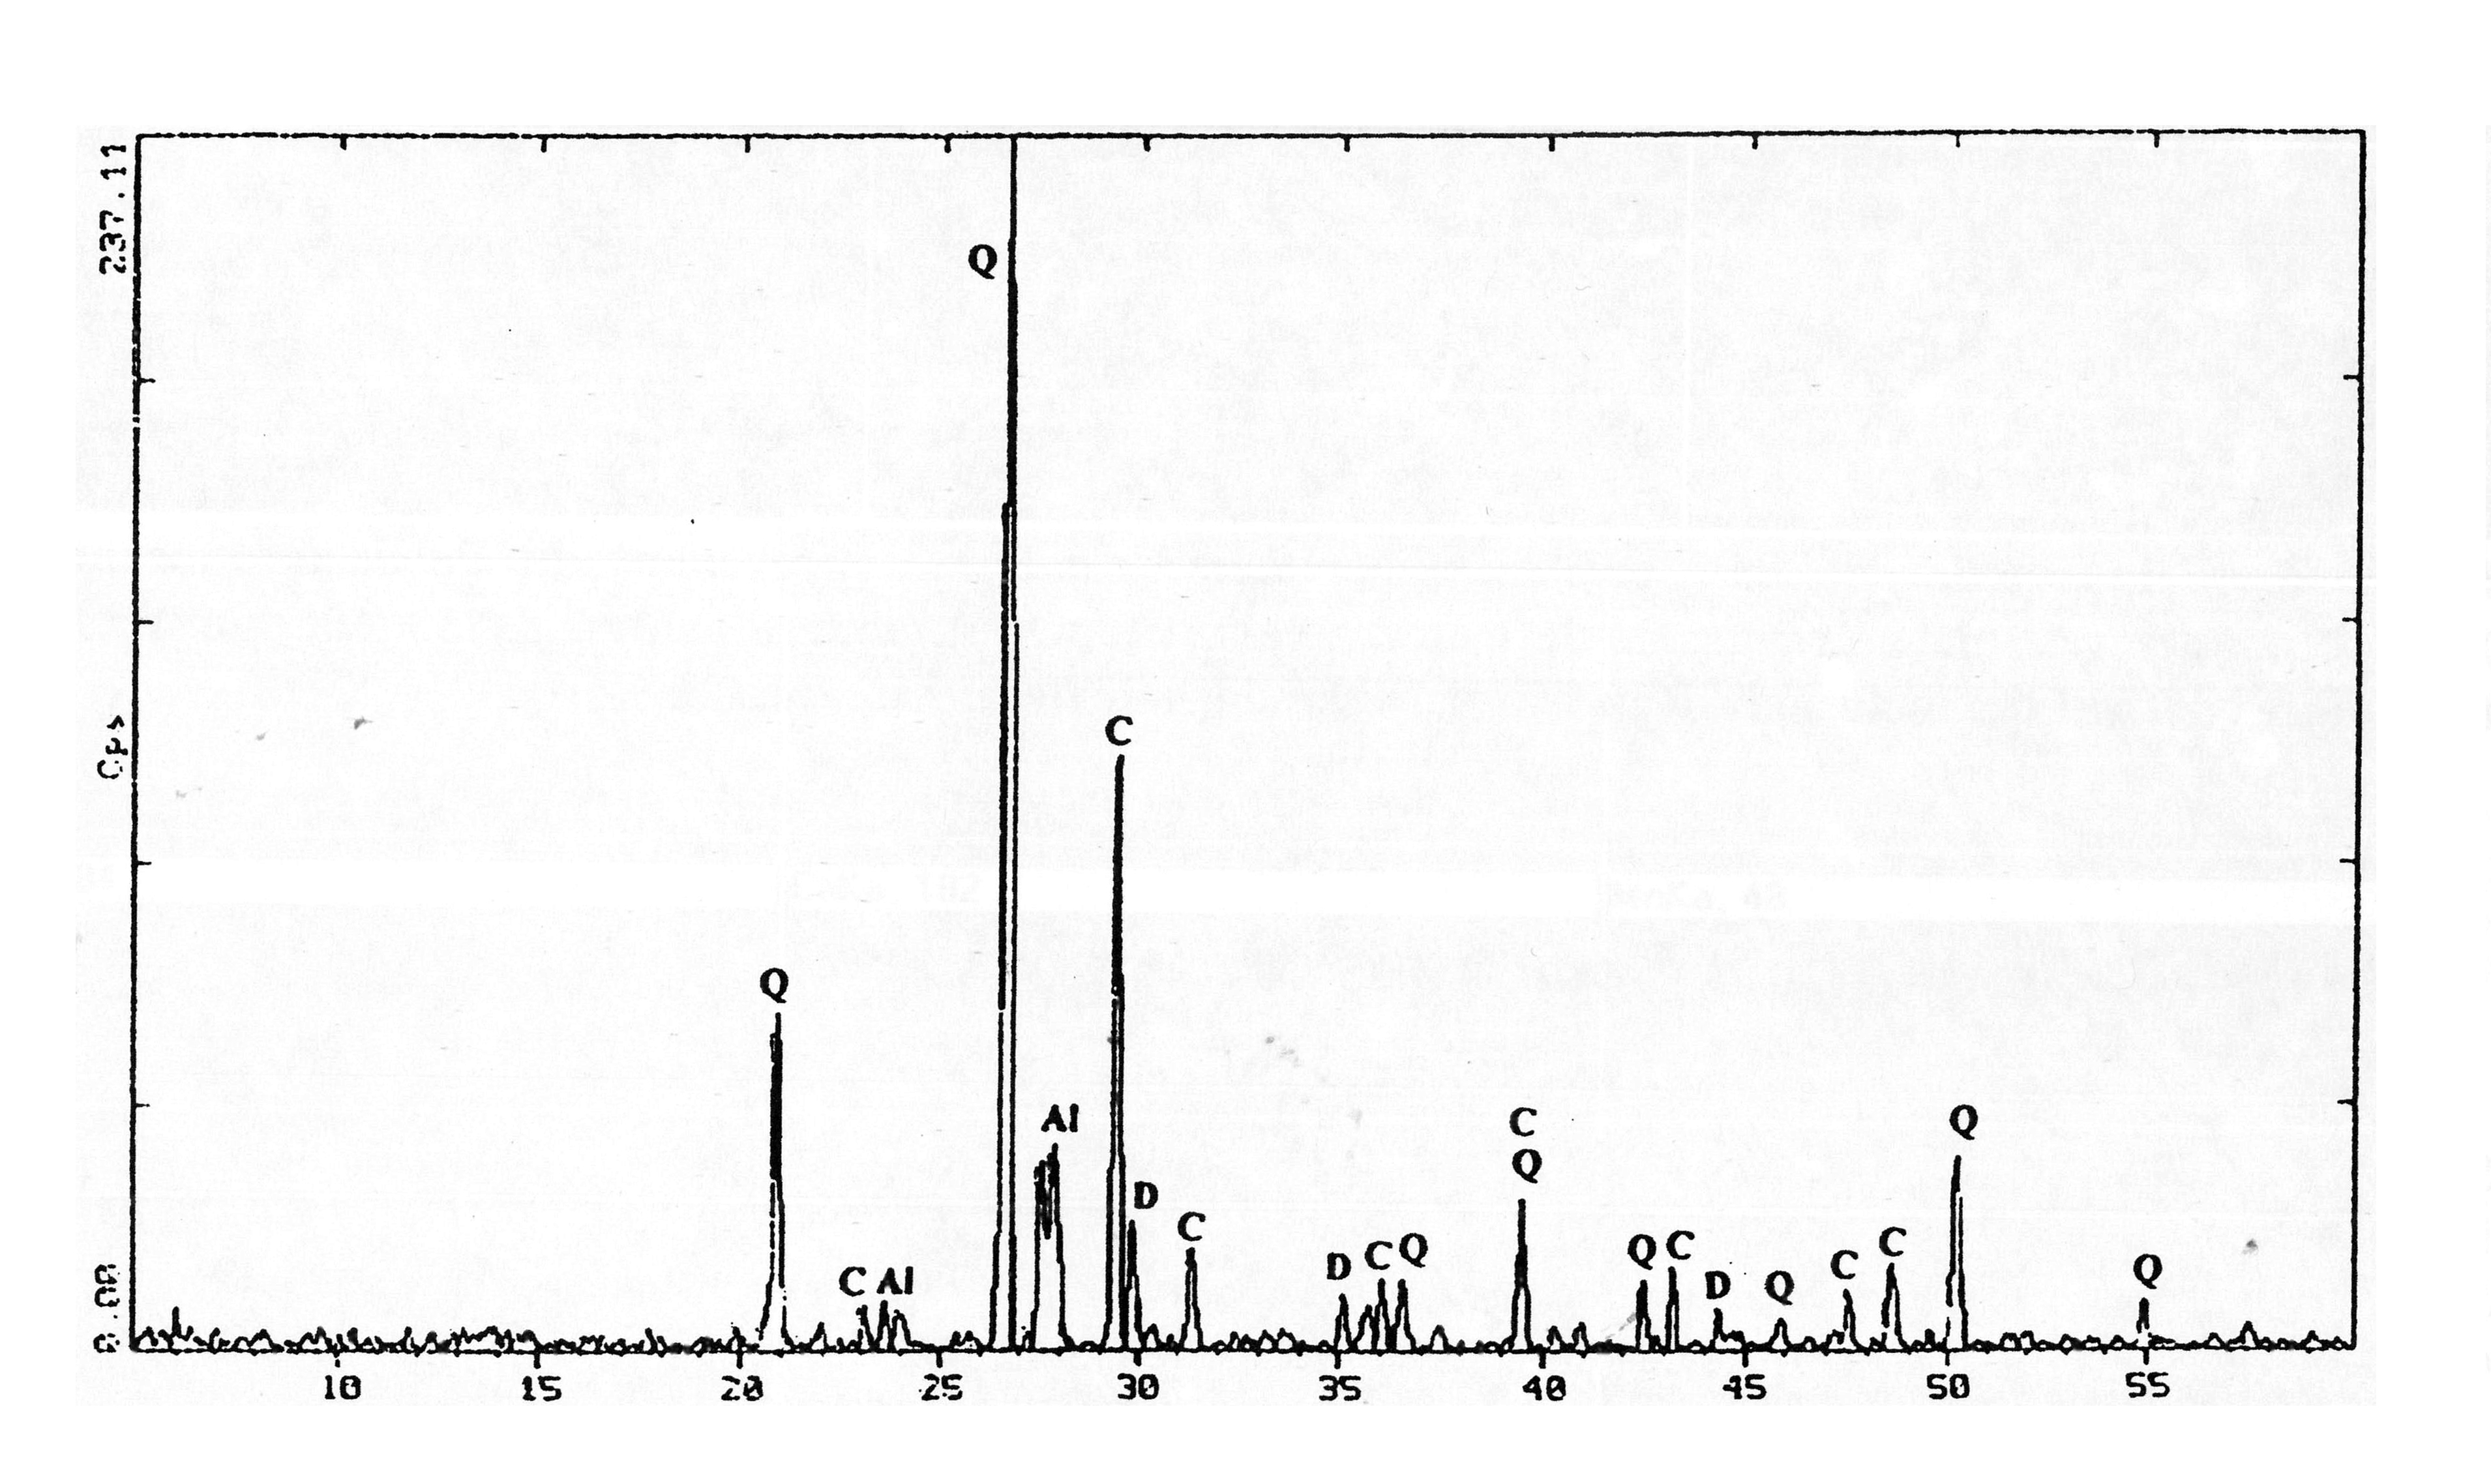
\includegraphics[width=\textwidth]{PaM_BDX6530_DX}
  \caption[\bdx{6530}\ -- \DX sur poudre de la terre cuite]
          {\legendeC 
           \DX sur poudre de la terre cuite. 
           Mise en évidence de la présence de quartz (Q), calcite (C), 
           albite (Al), diopside (D).}
  \label{DRX:6530}
\end{figure}

Le principal composé cristallisé mis en évidence par \DX sur poudre (\fref{DRX:6530}) est le quartz (\ce{SiO2}). La terre cuite contient également de la calcite (\ce{CaCO3}), responsable des luminescences rouges détectées en \CL. L'albite (\ce{NaAlSi3O8}) et le diopside (\ce{CaMg(SiO3)2}) sont également détectés.

La présence simultanée d'albite et du diopside, une phase haute 
température, laisse supposer que la température maximale de cuisson 
de la céramique a été de l'ordre de \SIrange{850}{900}{\degC}.


\section{Sur la présence et l'identification de cristaux de 
         dévitrification}
%----------------------------------------------------------------------

\subsection{Cristaux se développant dans la masse de la glaçure}
%~~~~~~~~~~~~~~~~~~~~~~~~~~~~~~~~~~~~~~~~~~~~~~~~~~~~~~~~~~~~~~~~~~~~~~
Ces cristaux aciculaires (\fref{MEB:6530_img_cxgla}) ont été 
identifiés par cartogarphie de \RX (\fref{MEB:6530_carto_cxgla}) et 
par des analyses ponctuelles (\tref{compelem:6530_cxgla}).

\begin{table}
  \begin{cartotab}
      \cartolgn{SiO2}{51.64}{0.75} &
      \cartolgn{CaO}{21.25}{2.08}  &
      \cartolgn{Al2O3}{1.95}{0.46} &
      \cartolgn{MgO}{2.83}{0.36}
    \tabularnewline
      \cartolgn{Na2O}{0.19}{0.07} &
      \cartolgn{K2O}{1.30}{0.32}  &
      \cartolgnnd{Fe2O3}          &
      \cartolgn{PbO}{7.97}{1.01}
    \tabularnewline
      \cartolgnnd{SnO2} &
      \cartolgnnd{CuO}  &
      \cartolgnnd{CoO}  &
      \cartolgn{MnO}{12.50}{0.64}
    \tabularnewline
      \cartolgnnd{Cr2O3} &
      \cartolgnnd{ZnO}   &
      \cartolgnnd{Sb2O3} &
      \cartolgnnd{TiO2}
    \tabularnewline
      \cartolgn{S}{0.23}{0.05} &
      \cartolgnnd{P2O5}        &
      \cartolgnnd{Cl}          &
      \cartolgnnd{As2O3}
    \tabularnewline
  \end{cartotab}
  \caption[\bdx{6530}\ -- Analyse quantitative par \EDS, composition élémentaire des 
           cristaux se développant dans la glaçure]
          {\legendeA Analyse quantitative par \EDS. Composition élémentaire des cristaux 
           se développant dans la glaçure par analyses ponctuelles 
           (\SI{1}{\um\squared}) (\PMO).}
  \label{compelem:6530_cxgla}
\end{table}

\begin{figure}[htb]
  \fakeimg{Carto RX cristaux glaçure (fig 48)}
  \caption[\bdx{6530}\ -- \carto de \RX des cristaux se développant dans la glaçure]
          {\legendeC 
           \carto de \RX des cristaux se développant dans la glaçure (Gr=2000, \zone{55x45}{\um}). Ces cristaux sont riches en calcium et manganèse.}
  \label{MEB:6530_carto_cxgla}
\end{figure}

Ce sont des silicates calciques de manganèse et de plomb. Leurs formes 
indiquent qu'il s'agit de cristaux de néoformation.

\begin{figure}[htb]
  \fakeimg{6530ER92 (fig 49)}
  \caption[\bdx{6530}\ -- Image en mode \ERD, cristaux aciculaires 
           se développant dans la masse de la glaçure]
          {\legendeC 
           Image en mode \ERD. Cristaux aciculaires se développant 
           dans la masse de la glaçure. La barre d'échelle mesure 
           \SI{10}{\um} (\zone{135x30}{\um}).}
  \label{MEB:6530_img_cxgla}
\end{figure}

\subsection{Cristaux se développant à l'interface}
%~~~~~~~~~~~~~~~~~~~~~~~~~~~~~~~~~~~~~~~~~~~~~~~~~~~~~~~~~~~~~~~~~~~~~~
Il s'agit de cristaux de dévitrification, de forme aciculaire, qui se 
développent pendant le refroidissement lent de la glaçure à partir de 
germes formés à haute température.

Nous avons réalisé des analyses ponctuelles pour en déterminer la 
composition élémentaire (\tref{compelem:6530_cx}).

\begin{table}
  \begin{cartotab}
      \cartolgn{SiO2}{55.47}{3.96}  &
      \cartolgn{CaO}{8.44}{2.15}    &
      \cartolgn{Al2O3}{16.57}{2.43} &
      \cartolgn{MgO}{2.26}{0.69}
    \tabularnewline
      \cartolgn{Na2O}{0.86}{0.34}  &
      \cartolgn{K2O}{6.39}{1.60}   &
      \cartolgn{Fe2O3}{5.07}{1.71} &
      \cartolgn{PbO}{3.59}{0.99}
    \tabularnewline
      \cartolgnnd{SnO2} &
      \cartolgnnd{CuO}  &
      \cartolgnnd{CoO}  &
      \cartolgn{MnO}{0.97}{0.23}
    \tabularnewline
      \cartolgnnd{Cr2O3} &
      \cartolgnnd{ZnO}   &
      \cartolgnnd{Sb2O3} &
      \cartolgn{TiO2}{0.39}{0.06}
    \tabularnewline
      \cartolgnnd{S}    &
      \cartolgnnd{P2O5} &
      \cartolgnnd{Cl}   &
      \cartolgnnd{As2O3}
    \tabularnewline
  \end{cartotab}
  \caption[\bdx{6530}\ -- Analyse quantitative par \EDS, composition élémentaire des 
           cristaux de dévitrification]
          {\legendeC Analyse quantitative par \EDS. Composition élémentaire des 
           cristaux de dévitrification par analyses ponctuelles
          (\SI{1}{\um\squared}) (\PMO).}
  \label{compelem:6530_cx}
\end{table}

Ces cristaux sont des aluminosilicates calco-potassiques. Ils 
contiennent également du fer.


\section{Étude des altérations de la glaçure}
%----------------------------------------------------------------------

Aucune figure d'altération n'a été mise en évidence dans la glaçure, 
ni visuellement, ni en \MEB[ie] (MEB).


\section{Bilan}
%----------------------------------------------------------------------

Cet échantillon est donc une pièce de céramique portant une glaçure 
plombifère dont la coloration \frquote{noire} est due au \ce{Mn^3+} 
associé au \ce{Fe^3+} en atmosphère de cuisson oxydante.

Son support de terre cuite est de type calcique. Sa coloration ocre-
rose est due à la présence de \ce{Fe^3+} en atmosphère de cuisson 
oxydante.

Sa composition \cristallo (quartz, calcite, albite, diopside) laisse penser qu'elle a été cuite à une température de l'ordre de \SIrange[range-phrase=\ à\ ]{850}{900}{\degC}.

À l'interface glaçure-terre cuite, on n'observe pas de luminescence. 
Cependant, cette zone renferme des cristaux de dévitrification 
identifiés comme des des aluminosilicates calco-potassiques contenant 
également du fer. Le faible développement de cette zone laisse 
envisager l'application du mélange glaçurant sur une terre cuite.

On note aussi la présence d'un autre type de cristaux de 
dévitrification dans la masse de la glaçure : des silicates calciques 
de manganèse et de plomb.

La glaçure ne présente pas de figure d'altération d'origine chimique 
mais une usure mécanique de surface.

%!TEX root = MemoireZelliges_simple.tex

\chapter{Étude physique d'un zellige miel (\bdx{6531})}
%======================================================================

\section{Description -- État de surface}
%----------------------------------------------------------------------

Cet échantillon, de forme parallélépipédique, est une pièce de 
céramique chanfreinée, comportant une glaçure miel 
(\fref{dessin:6531}). Il provient du \PaM (\siecle{xvii}) de Meknès.

\begin{itemize}
  \item \DimText : \SI{50x50x25}{\mm}
  \item \emph{Masse} : \SI{83.5}{\g}
\end{itemize}


\begin{figure}[htb]
  \begin{minipage}[t]{0.5\textwidth}
    \centerfloat
    \vspace*{0pt}
    % \fakeimg{Dessin de l'échantillon : Vue de dessus}
    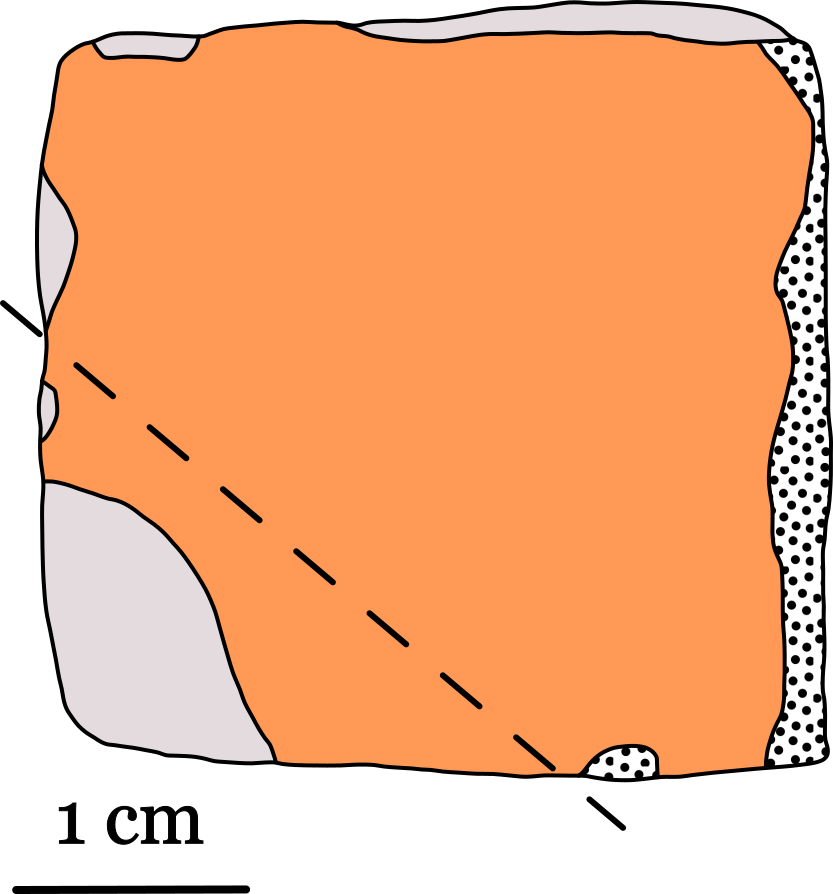
\includegraphics[scale=1]{PaM_BDX6531_dessus}
    \subcaption{Vue de dessus \label{dessin:6531_dessus}}
  \end{minipage}%
  \quad%
  \begin{minipage}[t]{0.5\textwidth}
    \centerfloat
    \vspace*{0pt}
    % \fakeimg{Dessin de l'échantillon : Lame}
    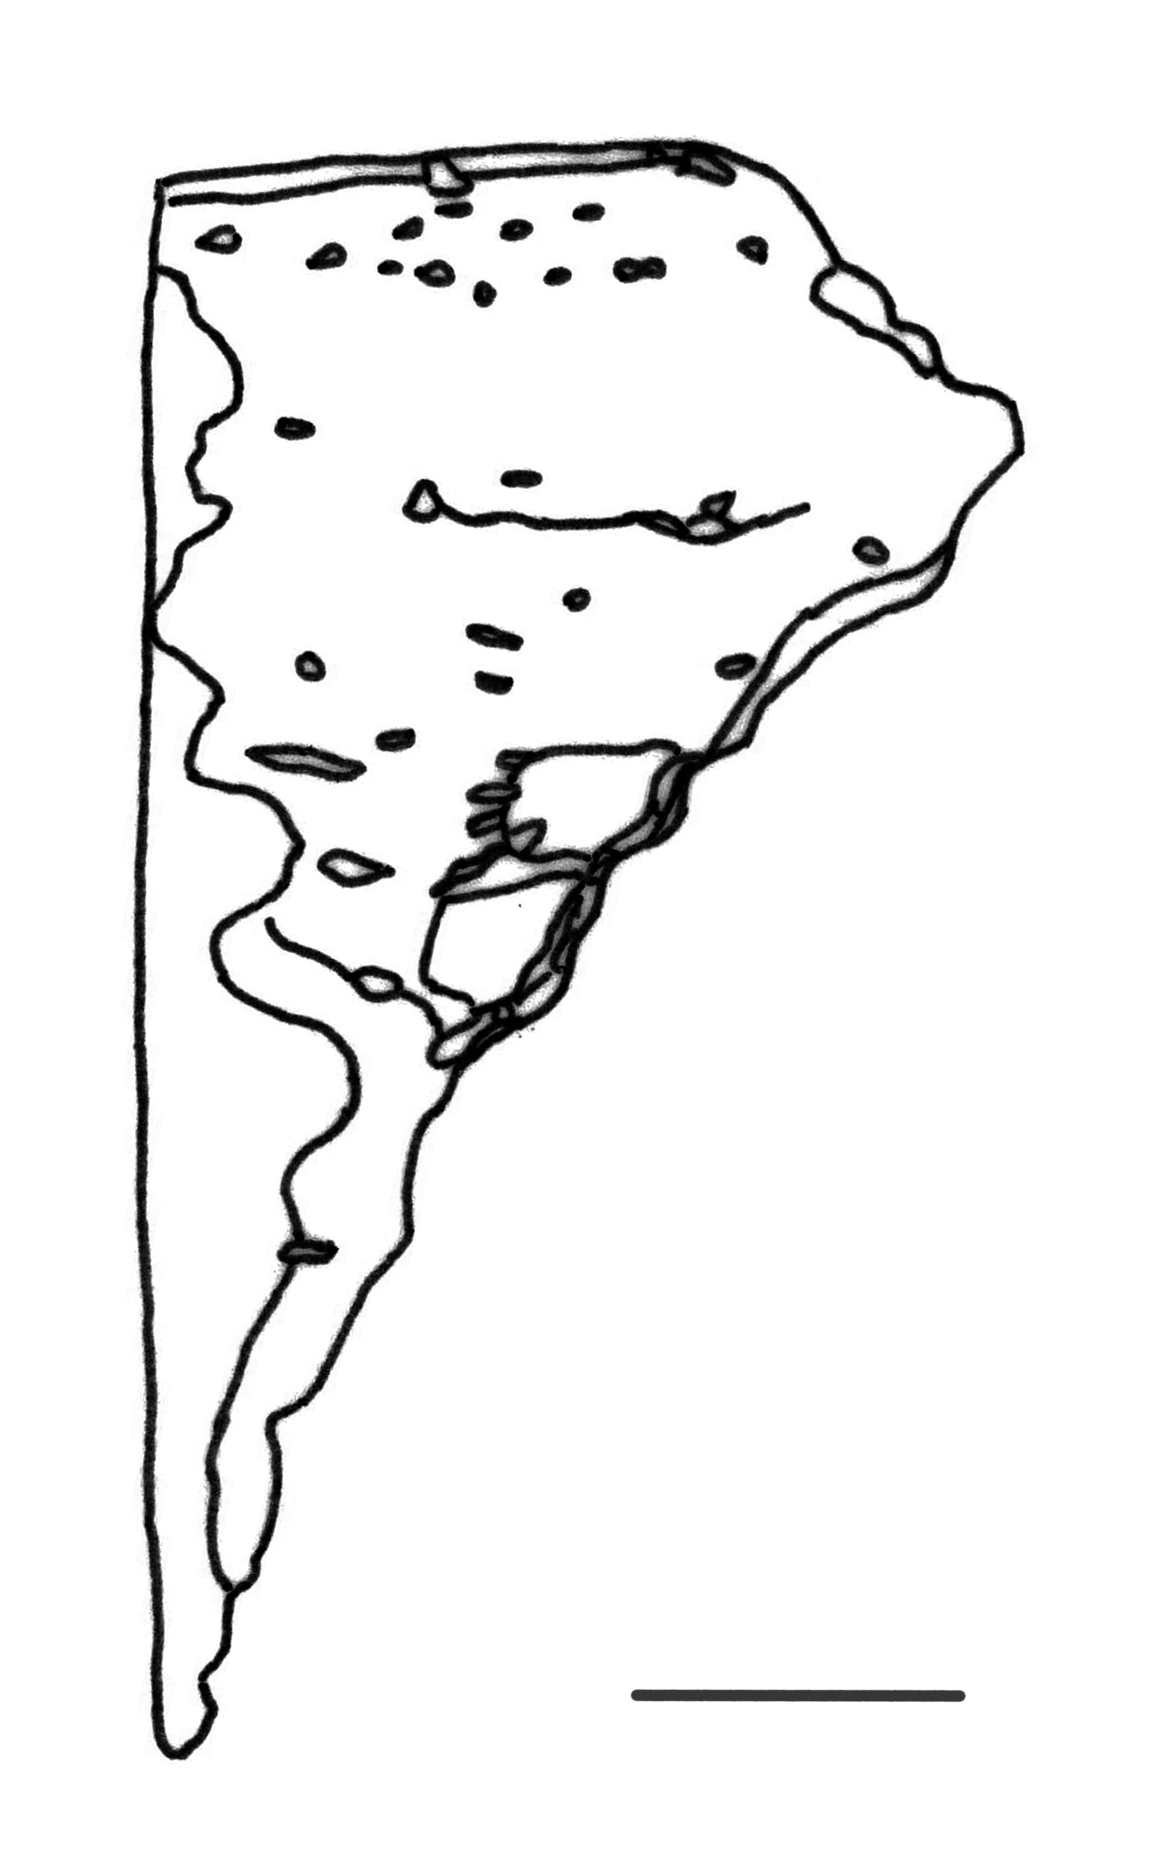
\includegraphics[scale=1]{PaM_BDX6531_lame}
    \subcaption{Lame étudiée \label{dessin:6531_lame}}
  \end{minipage}

  \bigskip

  \begin{minipage}[t]{0.5\textwidth}
    \centerfloat
    \vspace*{0pt}
    % \fakeimg{Dessin de l'échantillon : Coupe}
    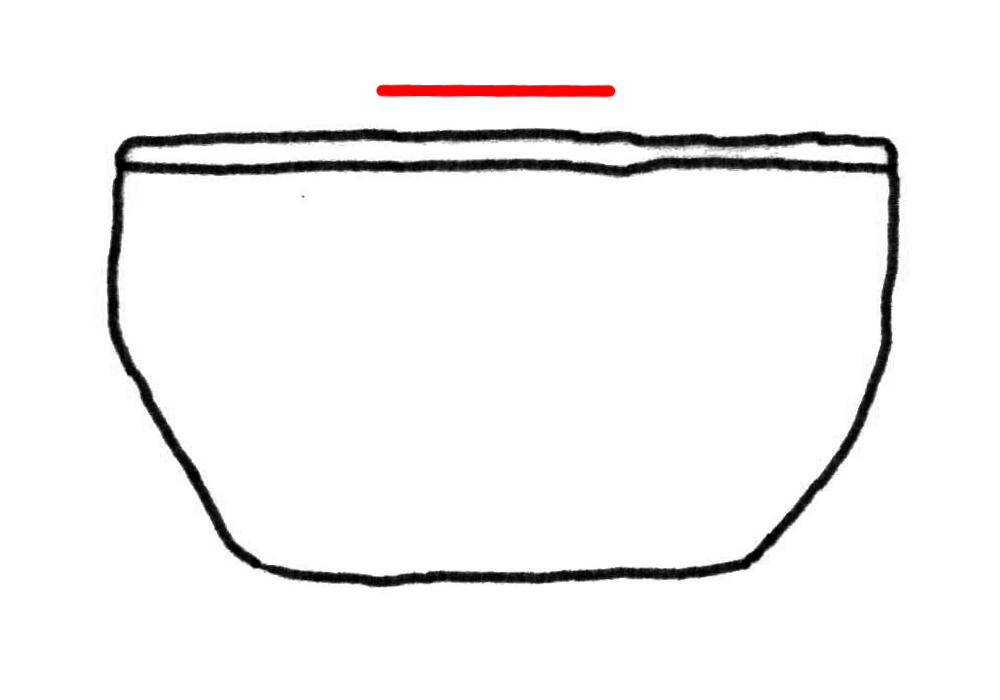
\includegraphics[scale=1]{PaM_BDX6531_coupe}
    \subcaption{Vue en coupe \label{dessin:6531_coupe}}
  \end{minipage}%
  \quad%
  \begin{minipage}[t]{0.5\textwidth}
    \vspace*{0pt}
    Légende :

    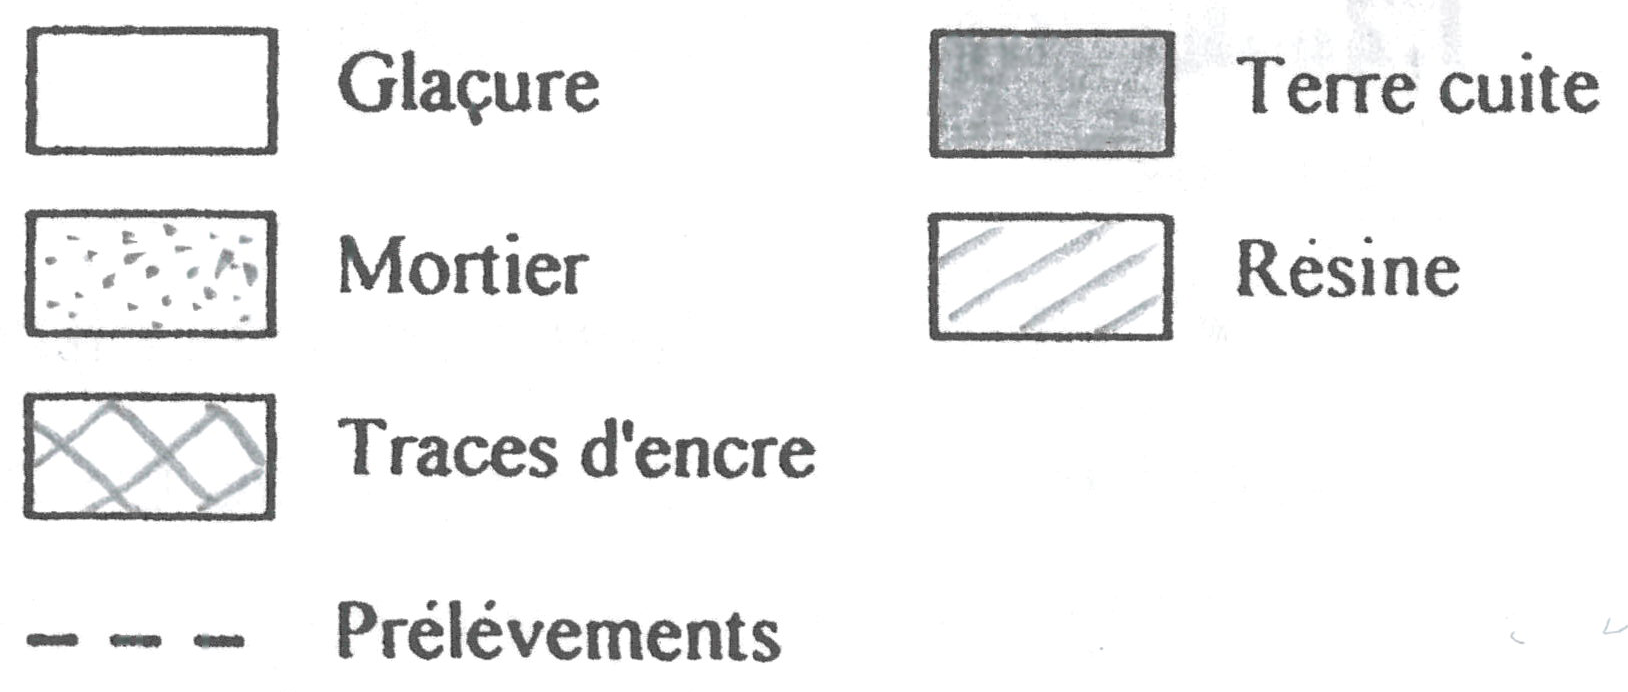
\includegraphics[scale=1]{dessin_legende}
    % \begin{itemize}
    %   \item Terre cuite
    %   \item Glaçure
    %   \item Résine
    %   \item Mortier
    %   \item Traces d'encre
    %   \item Prélévements
    % \end{itemize}
  \end{minipage}
  \caption{\legendeD}
  \label{dessin:6531}
\end{figure}

L'observation de la surface de la glaçure (\fref{surf:6531}) montre 
qu'elle contient des bulles, des picots et des cristaux non fondus.

Le support de terre cuite est de couleur ocre rosé, de granulométrie
fine, assez poreux et contient de nombreuses inclusions de tailles et
de couleurs variées.

\begin{figure}[htb]
  \includegraphics[width=\textwidth]{PaM_BDX6531_surf}
  \caption{\legendeD 
           État de surface de la glaçure (Gr=30, \zone{\sim4.3x3.2}{\mm}). Elle contient des bulles, des 
           picots et des cristaux non fondus.}
  \label{surf:6531}
\end{figure}


\section{Étude de la couleur}
%----------------------------------------------------------------------

\subsection{Identification des ions chromogènes}
%~~~~~~~~~~~~~~~~~~~~~~~~~~~~~~~~~~~~~~~~~~~~~~~~~~~~~~~~~~~~~~~~~~~~~~
\begin{figure}[htb]
  \begin{plotspectre}
    \addplot [thick, Orange] 
       table [x=lambda, y=6531gla] {\gladata} ;
    \addplot [thick, FireBrick] 
       table [x=lambda, y=6531tc] {\tcdata} ;
  \end{plotspectre}
  \caption{\legendeD 
           Spectres d'\AO en mode réflexion diffuse de la glaçure et de la terre cuite. La glaçure présente des absorptions vers \SIlist{380;440}{\nm}, correspondant au \ce{Fe^3+}.}
  \label{spectre:6531}
\end{figure}

Le spectre d'\AO en mode réflexion diffuse de la glaçure (\fref{spectre:6531}) présente une forte absorption à \SI{370}{\nm} et un épaulement à \SI{440}{\nm} attribuables au \ce{Fe^3+}. La terre cuite présente des épaulements à \SIlist{380;440}{\nm}, probablement attribuables au \ce{Fe^3+} ainsi qu'une bande d'absorption vers \SI{550}{\nm} qui n'a pu être attribuée.

\subsection{Mesure physique de la couleur}
%~~~~~~~~~~~~~~~~~~~~~~~~~~~~~~~~~~~~~~~~~~~~~~~~~~~~~~~~~~~~~~~~~~~~~~
Le \tref{saotab:6531} regroupe les coordonnées chromatiques, correspondant aux espaces \Yxy et \Lab, calculées à partir des spectres d'\AO de la glaçure et de la terre cuite.

La longueur d'onde dominante de la glaçure (\SI{579.24}{\nm}) 
correspond au domaine du jaune \autocite{Kelly_1976}. la couleur de 
la glaçure est foncée (réflectance $Y=\num{22.955}$) et assez saturée 
($P_e=\SI{43.65}{\percent}$). La \tref{saotab:6531} montre la 
localisation des coordonnées chromatiques de la glaçure dans les 
espaces \Yxy et \Lab. La couleur de la terre cuite se situe dans le 
domaine du jaune orange. Elle est assez claire, étant donnée sa 
réflectance ($Y=\num{38.927}$).

\begin{table}
  \begin{saotab}
      \saolgna{Glaçure}{579.24}{43.65}
              {22.955}{0.398}{0.400}
              {55.026}{4.617}{27.619} &
      \saolgnb{jaune foncé}{Jaune}{575}{580}{\footnotemark{}}
    \tabularnewline
      \saolgna{Terre cuite}{583.07}{27.15}
              {38.927}{0.372}{0.366}
              {68.698}{8.231}{19.231} &
      \saolgnb{jaune orange clair}{Jaune-Orange}{580}{585}
              {\footnotemark{}}
    \tabularnewline
  \end{saotab}
  \caption{\legendeD 
           Coordonnées chromatiques dans les systèmes \Yxy et \Lab 
           et longueur d'onde dominante (illuminant D65, \ang{2},
           \SIrange{400}{700}{\nm}).}
  \label{saotab:6531}
\end{table}
\footnotetext{\autocite{Kelly_1976}}
\footnotetext{\autocite{Kelly_1976}}

\begin{figure}[htb]
  \newcommand{\samplename}{6531gla}
  \newcommand{\samplecolor}{Orange}
  \begin{minipage}[t]{0.37\paperwidth}
    \begin{plotYxy}
      \plotYxyPaV ;
      \plotYxyIlluminant ;
      \plotYxySample{\samplename}{\samplecolor} ;
      \plotYxyLigne{\samplename} ;
      \plotYxyAnnot{\samplename}{south west} ;
    \end{plotYxy}
    \subcaption{espace \trichro \Yxy. La longueur d'onde 
                dominante de la glaçure est de \SI{594.38}{\nm} 
                et correspond au domaine des oranges.}
  \end{minipage}%
  \qquad%
  \begin{minipage}[t]{0.37\paperwidth}
    \begin{plotLab}
      \plotLabSample{\samplename}{\samplecolor} ;
    \end{plotLab}
    \subcaption{espace \trichro \Lab.}
  \end{minipage}%
  \caption[\bdx{6531}\ -- Espaces \trichro s]
          {\legendeD Analyse chromamétrique de la glaçure.}
  \label{colorfig:6531}
\end{figure}


\section{Étude de la texture de la glaçure et de la terre cuite sur 
         une section polie}
%----------------------------------------------------------------------

\subsection{Observation en lumière naturelle}
%~~~~~~~~~~~~~~~~~~~~~~~~~~~~~~~~~~~~~~~~~~~~~~~~~~~~~~~~~~~~~~~~~~~~~~
\begin{figure}[htb]
  \begin{minipage}[t]{0.4\textwidth}
    \fakeimg{lum. nat.}
    \subcaption{Lumière naturelle \label{texture:6531_LN}}
  \end{minipage}
  \begin{minipage}[t]{0.4\textwidth}
    \fakeimg{Cathodo}
    \subcaption{\CL \label{texture:6531_CL}}
  \end{minipage}
  \caption[\bdx{6531}\ -- Observation de la texture en section]
          {\legendeD 
           Observation de la texture en section sur une surface de 
           \SI{2.6x1.9}{\mm}.}
  \label{texture:6531}
\end{figure}

L'examen en section montre que la glaçure est transparente 
(\fref{texture:6531_LN}), colorée dans la masse et qu'elle 
adhère bien au support céramique. Ce dernier contient de nombreuses 
inclusions de faibles dimensions et de couleurs variées.

\subsection{Observation en \CL}
%~~~~~~~~~~~~~~~~~~~~~~~~~~~~~~~~~~~~~~~~~~~~~~~~~~~~~~~~~~~~~~~~~~~~~~
La glaçure n'est pas luminescente (\fref{texture:6531_CL}). 
On y observe des luminescences ponctuelles mauves.

La terre cuite présente une luminescence mauve à rose ainsi que 
quelques luminescences ponctuelles rouges et bleues.

On peut remarquer à l'interface glaçure/terre cuite des luminescences 
ponctuelles jaunes.

\subsection{Observation en \MEB[ie]}
%~~~~~~~~~~~~~~~~~~~~~~~~~~~~~~~~~~~~~~~~~~~~~~~~~~~~~~~~~~~~~~~~~~~~~~
La glaçure a une épaisseur moyenne de \SI{200}{\um}. Elle contient 
des cristaux non fondus de quartz (\ce{SiO2}), dont la dimension peut 
aller jusqu'à \SI{100}{\um}. Ils correspondent aux émissions 
ponctuelles mauves détectées en \CL (\fref{MEB:6531_img}).

\begin{figure}[htb]
  \fakeimg{Texture au MEB, retrodiff (fig 55)}
  \caption[\bdx{6531}\ -- Observation de la texture au \MEB, 
           en mode \ERD. Ensemble glaçure/terre cuite]
          {\legendeD 
           Observation de la texture au \MEB, en mode \ERD. 
           Ensemble glaçure/terre cuite. La barre d'échelle mesure 
           \SI{200}{\um} (\zone{680x550}{\um}).}
  \label{MEB:6531_img}
\end{figure}

Une \carto de \RX de l'ensemble glaçure-terre cuite (\fref{MEB:6531_carto_tcgla}) montre la présence de cristaux non fondus de quartz (\ce{SiO2}) dans la glaçure.

On observe très ponctuellement, à l'interface glaçure/terre cuite, la 
formation de cristaux de dévitrification de très petite taille. Cette 
zone semble assez riche en potassium et contient du plomb 
(\fref{MEB:6531_carto_tcgla}).

Le faible développement de cette zone d'interface laisse supposer des 
interactions faibles entre glaçure et terre cuite. L'hypothèse la plus 
probable est donc celle de l'application de la glaçure sur la terre 
cuite.

\begin{figure}[htb]
  \fakeimg{Texture au MEB, carto tc/gla (fig 56)}
  \caption[\bdx{6531}\ -- Observation de la texture au \MEB, \carto de \RX de l'ensemble glaçure/terre cuite]
          {\legendeD 
           Observation de la texture au \MEB, \carto de \RX de l'ensemble glaçure/terre cuite (Gr=140, \zone{770x625}{\um}).}
  \label{MEB:6531_carto_tcgla}
\end{figure}

\begin{figure}[htb]
  \fakeimg{Texture au MEB, carto tc (fig 57)}
  \caption[\bdx{6531}\ -- Observation de la texture au \MEB, \carto de \RX de la terre cuite]
          {\legendeD 
           Observation de la texture au \MEB, \carto de \RX de la terre cuite (Gr=140, \zone{770x625}{\um}).}
  \label{MEB:6531_carto_tc}
\end{figure}

La terre cuite contient des inclusions de quartz (\ce{SiO2}), 
d'alumino-silicates potassiques ainsi que des grains d'oxydes ou de 
carbonates de calcium (\fref{MEB:6531_carto_tc}).


\section{Composition élémentaire de la glaçure}
%----------------------------------------------------------------------

\begin{table}
  \begin{cartotab}
      \cartolgn{SiO2}{39.00}{1.27} &
      \cartolgn{CaO}{2.67}{0.20}   &
      \cartolgn{Al2O3}{1.04}{0.11} &
      \cartolgn{MgO}{0.39}{0.11}
    \tabularnewline
      \cartolgn{Na2O}{0.75}{0.08}  &
      \cartolgn{K2O}{1.45}{0.08}   &
      \cartolgn{Fe2O3}{3.95}{0.43} &
      \cartolgn{PbO}{50.34}{0.98}
    \tabularnewline
      \cartolgnnd{SnO2} &
      \cartolgnnd{CuO}  &
      \cartolgnnd{CoO}  &
      \cartolgnnd{MnO}
    \tabularnewline
      \cartolgnnd{Cr2O3} &
      \cartolgnnd{ZnO}   &
      \cartolgnnd{Sb2O3} &
      \cartolgn{TiO2}{0.19}{0.02}
    \tabularnewline
      \cartolgnnd{S}            &
      \cartolgnnd{P2O5}         &
      \cartolgn{Cl}{0.20}{0.09} &
      \cartolgnnd{As2O3}
    \tabularnewline
  \end{cartotab}

  \caption[\bdx{6531}\ -- Analyse quantitative par \EDS, composition élémentaire de la 
           glaçure]
          {\legendeD Analyse quantitative par \EDS. Composition élémentaire de la glaçure 
           miel sur une surface de \SI{54x44}{\um} (\PMO).}
  \label{compelem:6531_gla}
\end{table}

Il s'agit d'une glaçure plombifère non opacifiée 
(\tref{compelem:6531_gla}). C'est le fer, sous la forme~\ce{Fe^3+}, 
qui lui donne sa coloration miel.


\section{Étude de la terre cuite support}
%----------------------------------------------------------------------

\subsection{Composition élémentaire}
%~~~~~~~~~~~~~~~~~~~~~~~~~~~~~~~~~~~~~~~~~~~~~~~~~~~~~~~~~~~~~~~~~~~~~~
\begin{table}
  \begin{cartotab}
      \cartolgn{SiO2}{60.58}{4.99}  &
      \cartolgn{CaO}{17.68}{1.82}   &
      \cartolgn{Al2O3}{10.93}{1.68} &
      \cartolgn{MgO}{2.33}{0.17}
    \tabularnewline
      \cartolgn{Na2O}{0.45}{0.09}  &
      \cartolgn{K2O}{1.46}{0.25}   &
      \cartolgn{Fe2O3}{5.65}{1.00} &
      \cartolgnnd{PbO}
    \tabularnewline
      \cartolgnnd{SnO2} &
      \cartolgnnd{CuO}  &
      \cartolgnnd{CoO}  &
      \cartolgnnd{MnO}
    \tabularnewline
      \cartolgnnd{Cr2O3} &
      \cartolgnnd{ZnO}   &
      \cartolgnnd{Sb2O3} &
      \cartolgn{TiO2}{0.60}{0.09}
    \tabularnewline
      \cartolgn{S}{0.33}{0.03} &
      \cartolgnnd{P2O5}        &
      \cartolgnnd{Cl}          &
      \cartolgnnd{As2O3}
    \tabularnewline
  \end{cartotab}
  \caption[\bdx{6531}\ -- Analyse quantitative par \EDS, composition élémentaire de la terre cuite]
          {\legendeD Analyse quantitative par \EDS. Composition élémentaire de la terre cuite sur une surface de \SI{1080x876}{\um} (\PMO).}
  \label{compelem:6531_tc}
\end{table}

La terre cuite est riche en calcium (\tref{compelem:6531_tc}). C'est 
le \ce{Fe^3+} en atmosphère de cuisson oxydante qui lui donne sa 
coloration ocre rosé \autocite{Echallier_1984}.

\subsection{Composition \cristallo}
%~~~~~~~~~~~~~~~~~~~~~~~~~~~~~~~~~~~~~~~~~~~~~~~~~~~~~~~~~~~~~~~~~~~~~~
\begin{figure}[htb]
  \includegraphics[width=\textwidth]{PaM_BDX6531_DX}
  \caption[\bdx{6531}\ -- \DX sur poudre de la terre cuite]
          {\legendeA 
           \DX sur poudre de la terre cuite. 
           Mise en évidence de la présence de quartz (Q), calcite (C), 
           albite (Al), gehlénite (G), anorthite (A).}
  \label{DRX:6531}
\end{figure}

Le principal composé cristallisé mis en évidence par \DX sur poudre (\fref{DRX:6531}) est le quartz (\ce{SiO2}). On relève également la présence, à des teneurs plus faibles, de calcite (\ce{CaCO3}) pouvant correspondre aux émissions rouges détectées en \CL, de gehlénite (\ce{Ca2Al2SiO7}) et, probablement d'albite (\ce{NaAlSi3O8}) et d'anorthite (\ce{CaAl2Si2O8}). La très faible intensité des raies de ces derniers en rend l'indexation incertaine. Les feldspaths calciques peuvent être responsables des émissions bleues détectées en \CL.

La gehlénite et l'anorthite sont deux phases se développant à 
haute température. Leur présence laisse supposer que la température 
de cuisson de la pâte céramique a atteint 
\SIrange[range-phrase=\ à\ ]{850}{900}{\degC} \autocite{Peters_1978}.


\section{Sur la présence et l'identification de cristaux de 
         dévitrification}
%----------------------------------------------------------------------

On distingue, dans la zone d'interface terre cuite/glaçure, des 
cristaux de forme aciculaire. Ce sont des cristaux de dévitrification 
dont la composition élémentaire n'a pu être déterminée étant données 
leurs faibles dimensions.


\section{Étude des altérations de la glaçure}
%----------------------------------------------------------------------

Aucune figure d'altération n'a été mise en évidence dans la glaçure, 
ni visuellement, ni en \MEB[ie] (MEB).


\section{Bilan}
%----------------------------------------------------------------------

Cet échantillon est donc une pièce de céramique portant une glaçure 
plombifère dont la coloration miel est due au \ce{Fe^3+} en atmosphère 
de cuisson oxydante.

Son support de terre cuite est de type calcique. Sa coloration 
ocre-rose est due à la présence de \ce{Fe^3+} en atmosphère de 
cuisson oxydante.

Sa composition \cristallo (quartz, calcite, albite, gehlénite, anorthite) laisse penser qu'elle a été cuite à une température de l'ordre de \SIrange[range-phrase=\ à\ ]{850}{900}{\degC}.

À l'interface glaçure-terre cuite, on distingue des luminescences 
ponctuelles jaunes, associées à la présence de cristaux de 
dévitrification dont les faibles dimensions n'ont pas permis de 
déterminés la composition élémentaire. Le faible développement de 
cette zone laisse envisager l'application du mélange glaçurant sur 
une terre cuite.

La glaçure ne présente pas de figure d'altération d'origine chimique 
mais une usure mécanique de surface.

%!TEX root = MemoireZelliges_simple.tex

\chapter{Étude physique d'un zellige blanc (\bdx{6532})}
%======================================================================

\section{Description -- État de surface}
%----------------------------------------------------------------------

Cet échantillon (\fref{dessin:6532}), de forme parallélépipédique, 
est une pièce de céramique glaçurée de couleur blanche. Il provient 
du \PaM (\siecle{xvii}) de Meknès. Il est chamfreiné. Les traces 
d'encre violacée résultent de l'indexation de l'échantillon au Maroc.

\begin{itemize}
  \item \DimText : \SI{55x50x20}{\mm}
  \item \emph{Masse} : \SI{76.0}{\g}
\end{itemize}


\begin{figure}[htb]
  \begin{minipage}[t]{0.5\textwidth}
    \centerfloat
    \vspace*{0pt}
    % \fakeimg{Dessin de l'échantillon : Vue de dessus}
    \includegraphics[scale=1]{PaM_BDX6532_dessus}
    \subcaption{Vue de dessus \label{dessin:6532_dessus}}
  \end{minipage}%
  \quad%
  \begin{minipage}[t]{0.5\textwidth}
    \centerfloat
    \vspace*{0pt}
    % \fakeimg{Dessin de l'échantillon : Lame}
    \includegraphics[scale=1]{PaM_BDX6532_lame}
    \subcaption{Lame étudiée \label{dessin:6532_lame}}
  \end{minipage}

  \bigskip

  \begin{minipage}[t]{0.5\textwidth}
    \centerfloat
    \vspace*{0pt}
    % \fakeimg{Dessin de l'échantillon : Coupe}
    \includegraphics[scale=1]{PaM_BDX6532_coupe}
    \subcaption{Vue en coupe \label{dessin:6532_coupe}}
  \end{minipage}%
  \quad%
  \begin{minipage}[t]{0.5\textwidth}
    \vspace*{0pt}
    Légende :

    \includegraphics[scale=1]{dessin_legende}
    % \begin{itemize}
    %   \item Terre cuite
    %   \item Glaçure
    %   \item Résine
    %   \item Mortier
    %   \item Traces d'encre
    %   \item Prélévements
    % \end{itemize}
  \end{minipage}
  \caption{\legendeE}
  \label{dessin:6532}
\end{figure}

L'observation de la surface de la glaçure (\fref{surf:6532}) montre 
qu'elle contient des bulles, des picots, présente des rayures et 
contient des cristaux non fondus.

Le support de terre cuite est de couleur rosé, de granulométrie 
fine, peu poreux et contient de nombreuses inclusions de tailles 
et de couleurs variées.

\begin{figure}[htb]
  \includegraphics[width=\textwidth]{PaM_BDX6532_Surf}
  \caption{\legendeE 
           État de surface de la glaçure (Gr=30, \zone{\sim4.3x3.2}{\mm}). Elle contient des bulles, des 
           picots, des cristaux non fondus et présente des rayures.}
  \label{surf:6532}
\end{figure}


\section{Étude de la couleur}
%----------------------------------------------------------------------

\subsection{Identification des ions chromogènes}
%~~~~~~~~~~~~~~~~~~~~~~~~~~~~~~~~~~~~~~~~~~~~~~~~~~~~~~~~~~~~~~~~~~~~~~
\begin{figure}[htb]
  \begin{plotspectre}
    \addplot [thick, LightGoldenrod] 
       table [x=lambda, y=6532gla] {\gladata} ;
    \addplot [thick, FireBrick] 
       table [x=lambda, y=6532tc] {\tcdata} ;
  \end{plotspectre}
  \caption{\legendeE 
           Spectre d'\AO en mode réflexion diffuse de la glaçure. Le spectre ne présente pas de bande d'absorption particulière dans le visible et ne permet donc pas l'identification d'éléments chromogènes particuliers.}
  \label{spectre:6532}
\end{figure}

Le spectre d'\AO en mode réflexion diffuse de la glaçure (\fref{spectre:6532}) montre une absorption faible dans l'ensemble du domaine du visible et ne permet pas l'identification d'éventuels éléments chromogènes.

\subsection{Mesure physique de la couleur}
%~~~~~~~~~~~~~~~~~~~~~~~~~~~~~~~~~~~~~~~~~~~~~~~~~~~~~~~~~~~~~~~~~~~~~~
Les coordonnées \trichro s correspondant aux espaces \Yxy et \Lab ont été calculées pour la glaçure et de la terre cuite, à partir de leurs spectres d'\AO (\tref{saotab:6532}). La longueur d'onde dominante de la glaçure ($\lambda_D=\SI{575.30}{\nm}$) correspond au domaine du jaune \autocite{Kelly_1976} et la pureté d'excitation indique une couleur peu saturée ($P_e=\SI{13.84}{\percent}$). L'apparence blanche de la glaçure est due à sa forte réflectance ($Y=\num{50.011}$).

La \fref{colorfig:6532} montre la localisation des coordonnées 
chromatiques de la glaçure dans les espaces \Yxy et \Lab.

La longueur d'onde dominante ($\lambda_D=\SI{581.15}{\nm}$) de la 
terre cuite correspond au jaune orange \autocite{Kelly_1976}. La 
pureté d'excitation est assez faible ($P_e=\SI{24.58}{\percent}$) 
et la réflectance assez élevée ($Y=\num{35.676}$), on peut donc 
parler d'une couleur claire.

\begin{table}
  \begin{chrotab}
      \chrolgna{Glaçure}{575.30}{13.84}
               {50.011}{0.336}{0.355}
               {76.076}{-0.635}{11.486} &
      \chrolgnb{Jaune clair}{Jaune}{575}{580}{\footnotemark{}}
    \tabularnewline
      \chrolgna{Terre cuite}{581.15}{24.58}
               {35.676}{0.370}{0.370}
               {66.272}{5.871}{19.355} &
      \chrolgnb{jaune orange clair}{jaune orange}{580}{585}
               {\footnotemark{}}
    \tabularnewline
  \end{chrotab}
  \caption{\legendeE 
           Coordonnées chromatiques dans les systèmes \Yxy et \Lab 
           et longueur d'onde dominante (illuminant D65, \ang{2},
           \SIrange{400}{700}{\nm}).}
  \label{saotab:6532}
\end{table}
\footnotetext{\autocite{Kelly_1976}}
\footnotetext{\autocite{Kelly_1976}}

\begin{figure}[htb]
  \newcommand{\samplename}{6532gla}
  \newcommand{\samplecolor}{LightGoldenrod}
  \begin{minipage}[t]{0.37\paperwidth}
    \begin{plotYxy}
      \plotYxyPaV ;
      \plotYxyIlluminant ;
      \plotYxySample{\samplename}{\samplecolor} ;
      \plotYxyLigne{\samplename} ;
      \plotYxyAnnot{\samplename}{south west} ;
    \end{plotYxy}
    \subcaption{espace \trichro \Yxy. La longueur d'onde 
                dominante de la glaçure est de \SI{575.300}{\nm}. 
                Elle est dans le domaine du jaune, la couleur est 
                assez peu saturée.}
  \end{minipage}%
  \qquad%
  \begin{minipage}[t]{0.37\paperwidth}
    \begin{plotLab}
      \plotLabSample{\samplename}{\samplecolor} ;
    \end{plotLab}
    \subcaption{espace \trichro \Lab. Le point représentatif de 
                la couleur de la glaçure est sur la ligne du jaune.}
  \end{minipage}%
  \caption[\bdx{6532}\ -- Espaces \trichro s]
          {\legendeE Analyse chromamétrique de la glaçure.}
  \label{colorfig:6532}
\end{figure}


\section{Étude de la texture de la glaçure et de la terre cuite sur 
         une section polie}
%----------------------------------------------------------------------

\subsection{Observation en lumière naturelle}
%~~~~~~~~~~~~~~~~~~~~~~~~~~~~~~~~~~~~~~~~~~~~~~~~~~~~~~~~~~~~~~~~~~~~~~
\begin{figure}[htb]
  \begin{minipage}[t]{0.4\textwidth}
    \fakeimg{lum. nat.}
    \subcaption{Lumière naturelle \label{texture:6532_LN}}
  \end{minipage}
  \begin{minipage}[t]{0.4\textwidth}
    \fakeimg{Cathodo}
    \subcaption{\CL \label{texture:6532_CL}}
  \end{minipage}
  \caption{\legendeE 
           Observation de la texture en section sur une surface de 
           \SI{2.6x1.9}{\mm}.}
  \label{texture:6532}
\end{figure}

L'examen en section (\fref{texture:6532_LN}) montre que la 
glaçure est opaque, colorée dans la masse et qu'elle adhère bien au 
support céramique. La terre cuite contient de nombreuses inclusions 
de tailles et de couleurs diverses, réparties de manière homogène.

La limite entre la glaçure et la terre cuite semble très nette.

\subsection{Observation en \CL}

La glaçure n'est pas luminescente (\fref{texture:6532_CL}). 
Cependant, on observe à sa surface des luminescences mauve.

La terre cuite présente une luminescence à dominante mauve ainsi que 
des luminescences ponctuelles rouges et bleues se répartissant de 
manière homogène dans tout le matériau.

On ne distingue aucune luminescence à l'interface terre cuite-glaçure.

\subsection{Observation en \MEB[ie]}
%~~~~~~~~~~~~~~~~~~~~~~~~~~~~~~~~~~~~~~~~~~~~~~~~~~~~~~~~~~~~~~~~~~~~~~
La glaçure (\fref{MEB:6532_img}) a une épaisseur moyenne de \SI{260}{\um}. Elle contient des bulles et des cristaux non fondus, identifiés comme des quartz par \carto de \RX (\fref{MEB:6532_carto_tcgla}) et analyses ponctuelles par \spectro de \RX.

\begin{figure}[htb]
  \fakeimg{Texture au MEB, retrodiff}
  \caption{\legendeE 
           Observation de la texture au \MEB, en mode \ERD. 
           Ensemble glaçure/terre cuite. La barre d'échelle mesure 
           \SI{200}{\um} (\zone{500x400}{\um}).}
  \label{MEB:6532_img}
\end{figure}

On remarque également des cristaux de quartz non fondus formant un liseré continu à la surface de la glaçure. Ils sont responsables de la luminescence mauve détectée dans cette zone en \CL.

En \carto de \RX (\fref{MEB:6532_carto_tcgla}), on distingue la répartition homogène de l'étain, sous forme de grains de cassitérite (\ce{SnO2}), dans toute la glaçure.

Des grains de quartz de faible granulométrie (\SI{\sim10}{\um}) ont pu être ajoutés au mélange glaçurant en même temps que la cassitérite. On peut penser qu'ils participent à l'opacification de la glaçure par un effet de diffusion de la lumière.

\begin{figure}[htb]
  \fakeimg{Texture au MEB, carto tc/gla}
  \caption{\legendeE 
           Observation de la texture au \MEB, \carto de \RX de l'ensemble glaçure/terre cuite (Gr=190, \zone{580x475}{\um}).}
  \label{MEB:6532_carto_tcgla}
\end{figure}

\begin{figure}[htb]
  \fakeimg{Texture au MEB, carto tc}
  \caption{\legendeE 
           Observation de la texture au \MEB, en mode \ERD. 
           Zone d'interface. La barre d'échelle mesure \SI{50}{\um} 
           (\zone{185x175}{\um}).}
  \label{MEB:6532_img_int}
\end{figure}

À l'interface glaçure-terre cuite (\fref{MEB:6532_img_int}), on 
distingue des cristaux de néoformation de forme aciculaire.

La terre cuite (\fref{MEB:6532_carto_tc}) contient des inclusions de 
quartz (\ce{SiO2}) et d'alumino-silicates calco-potassiques.

\begin{figure}[htb]
  Texture au MEB, carto tc (fig 25)
  \caption{\legendeE 
           Observation de la texture au \MEB, \carto de \RX de la terre cuite (Gr=140, \zone{785x640}{\um}).}
  \label{MEB:6532_carto_tc}
\end{figure}


\section{Composition élémentaire de la glaçure}
%----------------------------------------------------------------------

Le \tref{compelem:6532_gla} présente la composition élémentaire de 
la glaçure blanche obtenue par \EDS.

Il s'agit d'une glaçure plombifère (\SI{47.88}{\percent} de \ce{PbO}) 
opacifiée à l'étain (\SI{5.19}{\percent} de \ce{SnO2}). La très faible 
teneur en fer (\SI{0.90}{\percent} de \ce{Fe2O3}) ne suffit pas à 
colorer la glaçure.

\begin{table}
  \begin{cartotab}
      \cartolgn{SiO2}{38.59}{1.43} &
      \cartolgn{CaO}{3.77}{0.06}   &
      \cartolgn{Al2O3}{1.65}{0.15} &
      \cartolgn{MgO}{0.60}{0.04}
    \tabularnewline
      \cartolgn{Na2O}{0.28}{0.04}  &
      \cartolgn{K2O}{0.94}{0.06}   &
      \cartolgn{Fe2O3}{0.90}{0.13} &
      \cartolgn{PbO}{47.88}{1.43}
    \tabularnewline
      \cartolgn{SnO2}{5.19}{0.43} &
      \cartolgnnd{CuO}            &
      \cartolgnnd{CoO}            &
      \cartolgnnd{MnO}
    \tabularnewline
      \cartolgnnd{Cr2O3}          &
      \cartolgnnd{ZnO}            &
      \cartolgnnd{Sb2O3}          &
      \cartolgnnd{TiO2}
    \tabularnewline
      \cartolgnnd{S}              &
      \cartolgnnd{P2O5}           &
      \cartolgn{Cl}{0.22}{0.08}   &
      \cartolgnnd{As2O5}
    \tabularnewline
  \end{cartotab}
  \caption{\legendeE 
           Analyse quantitative par \EDS. Composition élémentaire de la glaçure blanche sur une surface de \SI{108x88}{\um} (\PMO).}
  \label{compelem:6532_gla}
\end{table}


\section{Étude de la terre cuite support}
%----------------------------------------------------------------------

\subsection{Composition élémentaire}
%~~~~~~~~~~~~~~~~~~~~~~~~~~~~~~~~~~~~~~~~~~~~~~~~~~~~~~~~~~~~~~~~~~~~~~
\begin{table}
  \begin{cartotab}
      \cartolgn{SiO2}{51.96}{1.62} &
      \cartolgn{CaO}{19.46}{0.96} &
      \cartolgn{Al2O3}{14.03}{0.61} &
      \cartolgn{MgO}{3.47}{0.27}
    \tabularnewline
      \cartolgn{Na2O}{0.53}{0.05} &
      \cartolgn{K2O}{1.43}{0.16} &
      \cartolgn{Fe2O3}{7.52}{0.36} &
      \cartolgnnd{PbO}
    \tabularnewline
      \cartolgnnd{SnO2} &
      \cartolgnnd{CuO} &
      \cartolgnnd{CoO} &
      \cartolgnnd{MnO}
    \tabularnewline
      \cartolgnnd{Cr2O3} &
      \cartolgnnd{ZnO} &
      \cartolgnnd{Sb2O3} &
      \cartolgn{TiO2}{0.81}{0.10}
    \tabularnewline
      \cartolgn{S}{0.15}{0.03} &
      \cartolgn{P2O5}{0.57}{0.23} &
      \cartolgn{Cl}{0.06}{0.02} &
      \cartolgnnd{As2O5}
    \tabularnewline
  \end{cartotab}
  \caption{\legendeE Analyse quantitative par \EDS. Composition élémentaire de la terre 
           cuite sur une surface de \SI{2160x1752}{\um} (\PMO).}
  \label{compelem:6532_tc}
\end{table}

La terre cuite (\tref{compelem:6532_tc}) est riche en calcium. 
Sa coloration ocre rosé est due au \ce{Fe^3+} (\SI{7.52}{\percent} 
de \ce{Fe2O3}) en atmosphère de cuisson oxydante 
\autocite{Echallier_1984}. Ici encore, c'est l'excès de fer, non 
piégé dans les phases haute température, qui colore la terre cuite.

\subsection{Composition \cristallo}
%~~~~~~~~~~~~~~~~~~~~~~~~~~~~~~~~~~~~~~~~~~~~~~~~~~~~~~~~~~~~~~~~~~~~~~
Le principal composé cristallisé mis en évidence par \DX sur poudre (\fref{DRX:6528}) est le quartz (\ce{SiO2}), responsable 
de la luminescence mauve de la terre cuite. On relève également la
présence, à des teneurs plus faibles, de calcite (\ce{CaCO3}) pouvant 
correspondre aux émissions rouges détectées en \CL, d'anorthite 
(\ce{CaAl2Si2O8}), de diopside alumineux 
(\ce{Ca(Mg{,}Al)(Si{,}Al)2O6}) et de gehlénite (\ce{Ca2Al2SiO7}). 
Ces trois derniers cristaux peuvent être responsables des émissions 
bleues détectées en \CL.

La présence d'anorthite, de diopside alumineux et de gehlénite, 
trois phases se développant à haute température, laisse penser que 
la température de cuisson maximale de la céramique se situe autour 
de \SIrange[range-phrase=\ à\ ]{900}{950}{\degC}.

\begin{figure}[htb]
  \includegraphics[width=\textwidth]{PaM_BDX6532_DX}
  \caption{\legendeE 
           \DX sur poudre de la terre cuite. 
           Mise en évidence de la présence de quartz (Q), calcite (C), 
           gehlénite (G), anorthite (A), diopside (D).}
  \label{DRX:6532}
\end{figure}


\section{Sur la présence et l'identification de cristaux de 
         dévitrification}
%----------------------------------------------------------------------

On distingue, dans la zone d'interface terre cuite/glaçure, des cristaux de forme aciculaire. Ce sont des cristaux de dévitrification croissant pendant le refroidissement lent de la glaçure à partir de germes formés à haute température. Des analyses ponctuelles par \EDS ont montré (\tref{compelem:6532_cx}) que ces cristaux sont des alumino-silicates de calcium et de plomb.

\begin{table}
  \begin{cartotab}
      \cartolgn{SiO2}{39.64}{3.68} &
      \cartolgn{CaO}{5.85}{0.63}   &
      \cartolgn{Al2O3}{4.02}{0.61} &
      \cartolgn{MgO}{0.80}{0.28}
    \tabularnewline
      \cartolgn{Na2O}{0.25}{0.10}  &
      \cartolgn{K2O}{1.07}{0.09}   &
      \cartolgn{Fe2O3}{1.83}{0.16} &
      \cartolgn{PbO}{43.92}{4.89}
    \tabularnewline
      \cartolgn{SnO2}{2.14}{1.39} &
      \cartolgnnd{CuO}            &
      \cartolgnnd{CoO}            &
      \cartolgnnd{MnO}
    \tabularnewline
      \cartolgnnd{Cr2O3} &
      \cartolgnnd{ZnO}   &
      \cartolgnnd{Sb2O3} &
      \cartolgn{TiO2}{0.24}{0.07}
    \tabularnewline
      \cartolgnnd{S}            &
      \cartolgnnd{P2O5}         &
      \cartolgn{Cl}{0.24}{0.11} &
      \cartolgnnd{As2O3}
    \tabularnewline
  \end{cartotab}
  \caption{\legendeE Analyse quantitative par \EDS. Composition élémentaire des cristaux 
           de dévitrification par analyses ponctuelles 
           (\SI{1}{\um\squared}) (\PMO).}
  \label{compelem:6532_cx}
\end{table}


\section{Étude des altérations de la glaçure}
%----------------------------------------------------------------------

Aucune figure d'altération n'a été mise en évidence dans la glaçure, 
ni visuellement, ni en \MEB[ie] (MEB).


\section{Bilan}
%----------------------------------------------------------------------

Cet échantillon est donc une pièce de céramique portant une glaçure 
plombifère dont la coloration blanche est due à une opacification à 
l'étain. La présence de fins cristaux non fondus de quartz à sa 
surface participe aussi à cette opacification.

Son support de terre cuite est de type calcique. Sa coloration 
ocre-rose est due à la présence de \ce{Fe^3+} en atmosphère de 
cuisson oxydante.

Sa composition \cristallo (quartz, calcite, diopside, gehlénite, anorthite) laisse penser qu'elle a été cuite à une température de l'ordre de \SIrange[range-phrase=\ à\ ]{900}{950}{\degC}.

À l'interface glaçure-terre cuite, on n'observe pas de luminescence. 
Cependant, cette zone renferme des cristaux de dévitrification 
identifiés comme des des alumino-silicates de calcium et de plomb. 
Le faible développement de cette zone laisse envisager l'application 
du mélange glaçurant sur une terre cuite.

La glaçure ne présente pas de figure d'altération d'origine chimique 
mais une usure mécanique de surface.

\part{Bilan et perspectives}
%!TEX root = MemoireZelliges_simple.tex

\chapter{Bilan}
%======================================================================

\section{Comparaison entre les cinq zelliges étudiés}
%----------------------------------------------------------------------

\subsection{Description -- Texture}
%~~~~~~~~~~~~~~~~~~~~~~~~~~~~~~~~~~~~~~~~~~~~~~~~~~~~~~~~~~~~~~~~~~~~~~
On peut distinguer deux groupes distincts d'échantillons : d'une part, le zellige bleu, \frquote{pavé} servant à cerner le décor, et d'autre part les quatre zelliges vert, miel, noir et blanc, éléments du décor à proprement parler.

Ils se différencient tout d'abord par leur taille : le zellige bleu est beaucoup plus grand et plus épais (\SI{\sim4}{\cm} d'épaisseur pour le bleu, \SI{\sim2}{\cm} pour les autres) que les autres. Son substrat de céramique est également beaucoup plus rouge que les quatre zelliges plus petits, que l'on qualifierait plutôt d'ocre rose.

Les glaçures des zelliges vert, miel, noir et blanc présentent toutes des cassures franches et bien nettes. En revanche, on peut remarquer des coulures du mélange glaçurant sur le support de céramique du zellige bleu, réparties de manière homogène sur ses quatre faces.

On peut donc supposer que, contrairement au quatre autres, le zellige bleu n'a pas subit de découpe après l'application du mélange glaçurant et sa cuisson. La répartition homogène des coulures semble même indiquer que, lors de cette cuisson, le zellige était posé à plat, face glaçurée vers le haut.

L'étude de la texture de l'ensemble terre cuite-glaçure en lumière naturelle et \CL confirme cette ségrégation entre le zellige bleu et les quatre autres. En effet, le support de céramique du zellige bleu contient de grosses inclusions blanches et rouges observables à l'{\oe}il nu ainsi que quelques porosités de grande taille, réparties aléatoirement dans toute sa masse. À la loupe binoculaire, la terre cuite paraît très fine. En revanche, les terres cuites des quatre autres zelliges ne contiennent pas d'inclusions visibles à l'{\oe}il nu et sont assez peu poreuses. C'est l'observation à la loupe binoculaire qui y révèle la présence de nombreuses inclusions de couleurs variées (rouges, blanches, noires) et de granulométrie très fine (\SI{\sim0.15}{\mm}) réparties de manière homogène. De plus, la limite entre la glaçure et la terre cuite est très nette pour les quatre \frquote{petits} zelliges alors qu'elle est floue pour le bleu. On peut même parler de \frquote{fusion} des deux matériaux.

En \CL, on voit qu'aucune des glaçures ne luminesce mais que certaines (blanche, bleue) contiennent des cristaux de quartz (\ce{SiO2}) luminesçant en mauve.

La terre cuite du zellige bleu présente une luminescence à dominante mauve. Les autres présentent également une luminescence à dominante mauve mais avec de nombreuses luminescences ponctuelles rouges et bleues. De plus, dans le cas du zellige bleu, il faut noter, à l'interface terre cuite-glaçure, un liseré large qui luminesce en jaune et qui correspond à une bande de terre cuite plus clair en lumière naturelle. Pour les autres, on ne détecte pas ou peu de luminescences dans la zone d'interface.

L'observation au \MEB a permis de montrer que les luminescences aux interfaces ont pour origine des cristaux de dévitrification (des alumino-silicates mixtes de potassium, calcium et plomb).

Le très fort développement de la zone d'interface glaçure-terre cuite du zellige bleu peut laisser supposer des interactions fortes entre ces deux matériaux et donc l'application du mélange glaçurant sur une terre crue.

Dans les quatre autres zelliges, on trouve également des cristaux de dévitrification qui sont, selon ??? (199?), caractéristiques de l'application du mélange glaçurant sur une terre crue. Cependant les re-créations faites au laboratoire par Loïc~\bsc{Portelette} (1999, DESS) sont en contradiction avec ces résultats. De plus, le faible développement de l'interface semble indiquer peu d'interactions entre ces deux matériaux et donc, plutôt application du mélange glaçurant sur une terre cuite.

\subsection{Compositions élémentaires des glaçures}
%~~~~~~~~~~~~~~~~~~~~~~~~~~~~~~~~~~~~~~~~~~~~~~~~~~~~~~~~~~~~~~~~~~~~~~
\begin{figure}
  \begin{tikzpicture}
    \pgfplotstableread{\datadir/SpectroRX/PaM_BDX_SRX_gla.dat}
                      {\gladata}
    \pgfplotstablesort[sort key={bilan}]{\glasorted}{\gladata}

    \begin{axis}[
      bilan,
      ybar=0pt, bar width=5pt,
      title=Glaçures, title style={at={(0.33,0.85)}},
      ylabel=\PMO,
      x filter/.code={
        \pgfplotstablegetelem{\coordindex}{bilan}\of{\glasorted}
        \ifnumless{\pgfplotsretval}{99}{%
          %
        }{%
          \def\pgfmathresult{}
        }
      },
      xtick={0, ..., 10},
      xticklabels={
        \ce{SiO2},
        \ce{CaO},
        \ce{MgO},
        \ce{Na2O},
        \ce{K2O},
        \ce{Al2O3},
        \ce{PbO},
        \ce{SnO2},
        \ce{Fe2O3},
        \ce{CuO},
        \ce{MnO}
      },
    ]
      \addplot [fill=PaleGreen] 
         table [x expr=\coordindex, y=6528val, y error=6528err] 
         {\glasorted} ;
      \addlegendentry{Zellige vert}
      \addplot [fill=PowderBlue] 
         table [x expr=\coordindex, y=6529val, y error=6529err] 
         {\glasorted} ;
      \addlegendentry{Zellige bleu}
      \addplot [fill=Indigo] 
         table [x expr=\coordindex, y=6530val, y error=6530err] 
         {\glasorted} ;
      \addlegendentry{Zellige noir}
      \addplot [fill=Orange] 
         table [x expr=\coordindex, y=6531val, y error=6531err] 
         {\glasorted} ;
      \addlegendentry{Zellige miel}
      \addplot [fill=LightGoldenrod] 
         table [x expr=\coordindex, y=6532val, y error=6532err] 
         {\glasorted} ;
      \addlegendentry{Zellige blanc}
    \end{axis}

  \end{tikzpicture}
  \caption{\legendeAll 
           Compositions élémentaires des glaçures par \EDS. Toutes les glaçures sont plombifères. La glaçure verte est colorée par le \ce{Cu^2+}, la glaçure noire par le \ce{Mn^3+} et \ce{Fe^3+}, la glaçure miel par le \ce{Fe^3+}, la glaçure bleue est colorée par le \ce{Co^2+} et légèrement opacifiée à l'étain, la glaçure blanche est opacifiée à l'étain.}
  \label{plot:compo_gla}
\end{figure}

La \fref{plot:compo_gla} montre les compositions élémentaires de l'ensemble des glaçures. On peut constater qu'elles sont toutes plombifères. Elles ont donc été cuites en atmosphère oxydante car une cuisson réductrice aurait eu pour effet de noircir la glaçure. Les éléments chromogènes utilisés sont très classiques : le cobalt, sous la forme \ce{Co^2+} (comme le montre la \SAO), colore la glaçure bleue, associé à un peu d'étain pour adoucir la couleur et masquer la terre cuite rouge ; la coloration verte est due au cuivre dans l'état d'oxydation~II (montré par \SAO) ; le \ce{Mn^3+} associé au \ce{Fe^3+} donne sa coloration \frquote{orange foncé} à la glaçure noire ; la glaçure blanche est opacifiée par l'étain présent sous forme de cassitérite (\ce{SnO2}) et probablement par les fins cristaux de quartz non fondus présents à sa surface.

Il est intéressant de noter la plus faible teneur en plomb de la glaçure noire. Cela suppose qu'elle a été cuite à une température plus élevée que les autres.

La glaçure bleue ne contient quasiment pas d'oxyde d'aluminium, connu pour augmenter la viscosité du mélange glaçurant. Cela pourrait expliquer la position, à plat, de l'échantillon pendant la cuisson de ce mélange. En effet, si l'échantillon avait été placé debout \incise{comme c'est souvent le cas pour gagner de la place} le mélange glaçurant n'aurait probablement pas pu adhérer au support de céramique et aurait coulé.

\subsection{Compositions élémentaires des terres cuites}
%~~~~~~~~~~~~~~~~~~~~~~~~~~~~~~~~~~~~~~~~~~~~~~~~~~~~~~~~~~~~~~~~~~~~~~
\begin{figure}[htb]
  \begin{tikzpicture}
    \pgfplotstableread{\datadir/SpectroRX/PaM_BDX_SRX_tc.dat}%
                      {\tcdata}
    \pgfplotstablesort[sort key={bilan}]{\tcsorted}{\tcdata}

    \begin{axis}[
      bilan,
      ybar=0pt, bar width=5pt,
      title=Terres cuites, title style={at={(0.5,0.85)}},
      ylabel=\PMO,
      x filter/.code={
        \pgfplotstablegetelem{\coordindex}{bilan}\of{\tcsorted}
        \ifnumless{\pgfplotsretval}{99}{%
          %
        }{%
          \def\pgfmathresult{}
        }
      },
      xtick={0, ..., 8},
      xticklabels={
        \ce{SiO2},
        \ce{CaO},
        \ce{MgO},
        \ce{Na2O},
        \ce{K2O},
        \ce{Al2O3},
        \ce{Fe2O3},
        \ce{TiO2},
      },
    ]
      \addplot [fill=PaleGreen] 
         table [x expr=\coordindex, y=6528val, y error=6528err] 
         {\tcsorted} ;
      \addlegendentry{Zellige vert}
      \addplot [fill=PowderBlue] 
         table [x expr=\coordindex, y=6529val, y error=6529err] 
         {\tcsorted} ;
      \addlegendentry{Zellige bleu}
      \addplot [fill=Indigo] 
         table [x expr=\coordindex, y=6530val, y error=6530err] 
         {\tcsorted} ;
      \addlegendentry{Zellige noir}
      \addplot [fill=Orange] 
         table [x expr=\coordindex, y=6531val, y error=6531err] 
         {\tcsorted} ;
      \addlegendentry{Zellige miel}
      \addplot [fill=LightGoldenrod] 
         table [x expr=\coordindex, y=6532val, y error=6532err] 
         {\tcsorted} ;
      \addlegendentry{Zellige blanc}
    \end{axis}

  \end{tikzpicture}

  \caption{\legendeAll 
           Compositions élémentaires des terres cuites par 
           \EDS. Les terres 
           cuites sont très homogènes : elles sont de type calcique 
           et colorées par le fer en cuisson oxydante.}
  \label{plot:compo_tc}
\end{figure}

On peut constater sur la \fref{plot:compo_tc} que toutes les terres 
cuites sont de type calcique et que leur coloration rouge à ocre rose 
est due au fer présent sous la forme \ce{Fe^3+} en atmosphère de 
cuisson oxydante. C'est en fait le fer en excès, non piégé par les 
phases haute température dont le développement est favorisé par la 
présence de calcium.

L'homogénéité de composition des terres cuites peut apparaître comme 
contradictoire avec les différences de texture observées en lumière 
naturelle, \CL et \MEB[ie]. On peut émettre l'hypothèse que tous les 
échantillons ont été préparés à partir de la même matière première 
qui aurait subit une préparation différente selon l'emploi qui en est 
fait. Pour le zellige bleu, qui n'est pas un élément de décor mais une 
pièce utilisée pour le cerner, l'argile aurait subit une préparation 
assez sommaire. En revanche, l'argile utilisée pour fabriquer les 
éléments de décor aurait pu subir une décantation pour éliminer les 
inclusions les plus grosses (qui fragiliseraient le matériau lors de 
sa découpe) et, éventuellement, l'ajout d'un dégraissant minéral pour 
ajuster la plasticité du matériau aux besoins de l'artisan.

La teneur en fer est à peu près la même pour tous les échantillons, 
la différence de couleur entre le zellige bleu et les quatre autres 
pourrait s'expliquer par une atmosphère de cuisson légèrement plus 
oxydante pour le zellige bleu.

\subsection{Compositions \cristallo s des terres cuites}
%~~~~~~~~~~~~~~~~~~~~~~~~~~~~~~~~~~~~~~~~~~~~~~~~~~~~~~~~~~~~~~~~~~~~~~
Le \tref{tab:cristallo} présente les compositions \cristallo s des terres cuites des cinq échantillons. Toutes contiennent majoritairement du quartz, ainsi que de la calcite et diverses phases haute température (diopside, gehlénite, anorthite). On note également, pour les zelliges bleu, noir et miel, la présence d'albite.

Cette dernière disparaît vers \SI{850}{\degC}. Son association avec des phases haute température laisse penser que ces échantillons ont été cuits à une température de l'ordre de \SIrange[range-phrase=\ à\ ]{850}{900}{\degC}. Les zelliges vert et blanc auraient été cuits à une température légèrement plus élevée, de l'ordre de \SIrange[range-phrase=\ à\ ]{900}{950}{\degC}.


\begin{table}[htb]
  \sisetup{
    range-phrase = -
  }
  \centerfloat
  \noindent\begin{tabularx}{\textwidth}{X*{5}{M{1.7cm}}}
      ~ & \textbf{Zellige vert} & \textbf{Zellige bleu} & 
          \textbf{Zellige noir} & \textbf{Zellige miel} & 
          \textbf{Zellige blanc}
    \tabularnewline
    \otoprule
      \textbf{Quartz} (\ce{SiO2}) & 
      \blackstar & \blackstar & \blackstar & \blackstar & \blackstar
    \tabularnewline
    % \midrule
      \textbf{Calcite} (\ce{CaCO3}) & 
      \blackstar & \blackstar & \blackstar & \blackstar & \blackstar
    \tabularnewline
    % \midrule
      \textbf{Albite} &
       ~         & \bluestar  & \bluestar  & \bluestar  & ~
    \tabularnewline
    % \midrule
      \textbf{Diopside} &
      \blackstar & \blackstar & \blackstar & ~          & \blackstar
    \tabularnewline
    % \midrule
      \textbf{Gehlénite} &
      \blackstar & \blackstar & ~          & \blackstar & \blackstar
    \tabularnewline
    % \midrule
      \textbf{Anorthite} &
      \blackstar & ~          & ~          & \blackstar & \blackstar
    \tabularnewline
    % \midrule
      \textbf{Température de \mbox{cuisson} associée} (\si{\degC}) & 
      \numrange{900}{950} & \numrange{850}{900} & 
      \numrange{850}{900} & \numrange{850}{900} & 
      \numrange{900}{950}
    \tabularnewline
    \bottomrule
\end{tabularx}
\caption{\legendeAll 
         Compositions \cristallo s des terres cuites.}
\label{tab:cristallo}
\end{table}

\subsection{Étude de l'altération}
%~~~~~~~~~~~~~~~~~~~~~~~~~~~~~~~~~~~~~~~~~~~~~~~~~~~~~~~~~~~~~~~~~~~~~~
Nous n'avons détectées de figures d'altération chimique, que ce soit 
en lumière naturelle ou en \MEB[ie], dans aucun des cinq échantillons 
étudiés. En revanche, les cinq échantillons présentent une plus ou 
moins prononcée usure mécanique de surface.


\section{Proposition d'un protocole technologique}
%----------------------------------------------------------------------

L'ensemble de ces données nous a permis de proposer des hypothèses 
quant aux techniques de fabrications des zelliges. Il y aurait en fait 
deux techniques différentes selon l'utilisation de l'échantillon. Ces 
techniques sont résumées dans la \fref{fig:protocole}.

Dans le cas des pièces de grandes dimensions telles que le zellige 
bleu, utilisées pour cerner le décor, le potier procéderait au moulage 
d'un \frquote{pavé} parallélépipédique (de l'ordre de \SI{4}{\cm} 
d'épaisseur) à partir d'une argile préparé de manière assez sommaire. 
Il appliquerait ensuite sur ce support le mélange glaçurant et 
l'ensemble serait enfin soumis à une cuisson en atmosphère oxydante 
à une une température de l'ordre de
\SIrange[range-phrase=\ à\ ]{900}{950}{\degC}.

La même pâte argileuse subirait une préparation plus élaborée pour la 
mise en {\oe}uvre des éléments du décor, avec décantation et ajout de 
dégraissant minéral. De grand carreaux sont ensuite moulés et 
subissent peut-être une première cuisson oxydante à 
\SIrange[range-phrase=\ à\ ]{850}{900}{\degC}. Le mélange glaçurant 
est ensuite appliqué et l'ensemble est alors soumis à une deuxième (ou 
première) cuisson oxydante. Le maître-artisan peut ensuite procéder à 
la découpe des formes voulues et à leur assemblage.


\begin{figure}[p]
  \large
  \begin{tikzpicture}[yscale=-1]
    \tikzset{
      every node/.style = {
        draw, rectangle, rounded corners, 
        font           = \smaller, 
        inner sep      = 1ex, 
        minimum height = 1cm, 
        minimum width  = 3.5cm,
        text width     = 3.5cm,
        align          = center
      },
      red/.style = {
        fill = gray!50!red!20, 
        minimum height = 1cm, 
        minimum width  = 9cm,
        text width     = 9cm,
      },
      blanc/.style = {
        minimum height = 1cm, 
        minimum width  = 1.4cm,
        text width     = 1.4cm,
      },
      bleu/.style = {
        fill = PowderBlue, 
        % fill = gray!50!blue!20, 
      },
      autre/.style = {
        fill = PaleGreen, 
        % fill = gray!50!green!20, 
      },
      flech/.style = {
        thick,
        ->,
        >=stealth,
      }
    }

    % \draw [help lines] (-8, 0) grid ( 8, 18) ;

    \node [red] (A) at ( 0.00, 0.00) 
          {Pâte argileuse calcique riche en fer} ;

    \node [blanc] (B0) at (-6.00, 1.00) 
          {Zellige bleu} ;
    \node [bleu]  (B1) at (-4.00,  3.00) 
          {Préparation sommaire} ;
    \node [bleu]  (B2) at (-4.00,  5.50) 
          {Moulage du pavé\\{\smaller(\SI{75x60x40}{\mm})}} ;
    \node [bleu]  (B4) at (-4.00,  8.50) 
          {Application du\\mélange glaçurant} ;
    \node [bleu]  (B5) at (-4.00, 11.00) 
          {Cuisson oxydante\\
           {\smaller(\SIrange[range-phrase=-]{900}{950}{\degC})}} ;

    \node [blanc] (C0) at ( 6.00,  1.00) 
          {Autres Zelliges} ;
    \node [autre] (C1) at ( 4.00,  3.00) 
          {Préparation élaborée\\
           {\smaller(décantation -- ajout de dégraissant)}} ;
    \node [autre] (C2) at ( 4.00,  5.50) 
          {Moulage de carreaux\\{\smaller(épaisseur : \SI{20}{\mm})}} ;
    \node [autre] (C3) at ( 6.50,  7.00) 
          {Cuisson oxydante ?\\
           {\smaller(\SIrange[range-phrase=-]{850}{950}{\degC})}} ;
    \node [autre] (C4) at ( 4.00,  8.50) 
          {Application du\\mélange glaçurant} ;
    \node [autre] (C5) at ( 4.00, 11.00) 
          {Cuisson oxydante} ;
    \node [autre] (C6) at ( 4.00, 13.50) 
          {Découpe des pièces} ;

    \node [red] (Z) at ( 0.00, 16.50) 
          {Assemblage du panneau de zelliges} ;

    \draw [flech] (A.200) to [out=90, in=-90] (B1.north) ;
    \draw [flech] (B1) -- (B2) ;
    \draw [flech] (B2) -- (B4) ;
    \draw [flech] (B4) -- (B5) ;
    \draw [flech] (B5.south) to [out=90, in=-90] (Z.160) ;

    \draw [flech] (A.-20) to [out=90, in=-90] (C1.north) ;
    \draw [flech] (C1) -- (C2) ;
    \draw [flech, dashed] (C2) -- (C4) ;
    \draw [flech] (C4) -- (C5) ;
    \draw [flech] (C5) -- (C6) ;
    \draw [flech] (C6.south) to [out=90, in=-90] (Z.20) ;
  \end{tikzpicture}
  \caption{Deux techniques de fabrications des zelliges à partir d'une 
           même argile calcique riche en fer. L'argile est préparée de 
           manière plus ou moins élaborée selon l'usage qu'il en est 
           fait.}
  \label{fig:protocole}
\end{figure}


\chapter{Perspectives}
%======================================================================

Notre étude a permis d'obtenir de nombreux indices sur les techniques 
de fabrication des zelliges de Meknès. Cependant, il reste encore des 
questions sans réponse (notamment, la question de l'application du 
mélange glaçurant sur terre crue ou cuite) et nos hypothèses doivent 
être vérifiées.

Il serait donc intéressant, pour valider ou infirmer notre proposition 
sur les techniques de fabrication des zelliges, de procéder à des 
essais de re-création en collaboration avec des céramistes et en 
utilisant des fours proches de ceux du \siecle{xvii} et des matières 
premières disponibles dans la région de Meknès.

Une étude comparative avec les échantillons de zelliges de Meknès 
datant du \siecle{xiv} étudiés cette année par Richard~\bsc{Cheret}, 
pourrait permettre d'obtenir des données sur l'évolution historique 
des techniques de fabrication de ce matériau. Il est nécessaire, pour 
cela, d'élargir l’échantillonnage à du matériel s'intercalant entre 
le \sclnum{xiv} et le \siecle{xvii} pour compléter cet 
\frquote{historique}.

Enfin, le deuxième volet de notre problématique de départ concernait 
l'altération des panneaux de zelliges qui se détachent en partie. Or, 
notre étude a montré que les zelliges eux-mêmes ne sont pas du tout 
altérés et ont bien résisté au temps. Il est donc nécessaire d'étudier 
les mortiers liant les pièces entre elles et permettant de maintenir 
le panneau au mur, puisque ce sont certainement eux qui sont 
responsables de ces dégradations.


\appendix
% \appendixpage

% \phantomsection
% \addcontentsline{toc}{book}{\appendixpagename}
% \book*{\appendixpagename}

\backmatter
\newpage
\listoffigures
\listoftables

\nocite{*}
\printbibliography[heading=memoir,title=Bibliographie]

\begin{tabular}{*{34}{c}}
    BDX\,\no & Nature & Photo & Dessin & DX & 
    Photo & Mavica & Num. & 
    Image & $\micro$fluo\,X & 
    \SI{77}{\kelvin} & l.onde & Image & 
    \SI{77}{\kelvin} & l.onde & Photo & Mavica & Num. &
    Spectro gamma & Chroma & ATD & Absorp optique & PL & 
    \SI{20}{\degC} & l.onde & Photo & 
    OSL & IRSL & \ce{He} &
    \SI{77}{\kelvin} & \SI{20}{\degC} & 
    \SI{77}{\kelvin} & \SI{20}{\degC} & Raman
  \tabularnewline
    6528 & céram. gla. & \texttimes & \texttimes & \texttimes & 
     & \texttimes & & 
    \texttimes & \texttimes & 
     & & & 
     & & \texttimes & &
     & & & \texttimes & & 
     & & & & & & & & & &
  \tabularnewline
    6529 & céram. gla. & \texttimes & \texttimes & \texttimes & 
     & \texttimes & & 
    \texttimes & \texttimes & 
     & & & 
     & & \texttimes & &
     & & & \texttimes & & 
     & & & & & & & & & &
  \tabularnewline
    6530 & céram. gla. & \texttimes & \texttimes & \texttimes & 
     & \texttimes & & 
    \texttimes & \texttimes & 
     & & & 
     & & \texttimes & &
     & & & \texttimes & & 
     & & & & & & & & & &
  \tabularnewline
    6531 & céram. gla. & \texttimes & \texttimes & \texttimes & 
     & \texttimes & & 
    \texttimes & \texttimes & 
     & & & 
     & & \texttimes & &
     & & & \texttimes & & 
     & & & & & & & & & &
  \tabularnewline
    6532 & céram. gla. & \texttimes & \texttimes & \texttimes & 
     & \texttimes & & 
    \texttimes & \texttimes & 
     & & & 
     & & \texttimes & &
     & & & \texttimes & & 
     & & & & & & & & & &
  \tabularnewline


\end{tabular}

\cleardoublepage
\pagestyle{empty}
~\newpage
%!TEX root = MemoireZelliges.tex

{
\large
\noindent\SL

\noindent DESS Méthodes Physiques Appliquées à l'Archéologie et à la 
Muséographie -- Juin 2000

\vfill

\begin{center}
\bfseries\Large
Programme PACT ARCHI-MED Glaçures -- II

\vspace*{-0.75\baselineskip}

\rule{.5\textwidth}{1pt}

\bigskip

\MakeUppercase{Contribution à la réhabilitation architecturale du 
\PaM, Meknès, Maroc, \siecle{17}}

\bigskip

Recherche des caractéristiques physiques de zelliges de pavement
\end{center}

\vfill

Le travail présenté ici s'intègre dans le cadre du programme 
\emph{PACT ARCHI-MED Glaçures} qui a pour but l'étude de la céramique 
glaçurée architecturale du monde méditerranéen. Cette étude porte sur 
cinq échantillons de zelliges (bleu, vert, miel, noir et blanc) 
provenant du \PaM de Meknès, \siecle{17}.

L'étude de la texture en section, en lumière naturelle et en \CL, 
a permis de mettre en évidence deux groupes d'échantillons se 
distinguant par la couleur de leur support céramique, la granulométrie 
des inclusions et la présence ou l'absence de liseré luminescent à 
l'interface glaçure/terre cuite : d'une part les zelliges vert, miel, 
noir et blanc, d'autre part, le zellige bleu, de plus grandes 
dimensions que les autres, avec un support céramique plus rouge, 
contenant des inclusions plus grossières. L'imagerie en \MEB[ie] donne 
accès à la microtexture des échantillons et permet de corréler un 
liseré qui luminesce en jaune en \CL à la présence de cristaux de 
dévitrification dans la zone d'interface terre cuite/glaçure.

L'analyse quantitative en \EDS montre la grande homogénéité des 
matériaux, tant des glaçures plombifères, que des terres cuites de 
type calcique, et permet de détecter la présence d'étain, utilisé 
comme opacifiant dans deux des cinq glaçures (blanche et bleue).

La présence de phases cristallines de haute température dans 
les terres cuites, détectées en \DX sur poudre peut donner des 
indications quant aux températures de cuisson atteintes, entre 
\SIrange[range-phrase=\ et\ ]{850}{950}{\degC}.

La \SAO nous a permis de déterminer les éléments chromogènes utilisés 
pour colorer les glaçures (bleue : \ch{Co^2+} ; verte : \ch{Cu^2+} 
dans une glaçure plombifère ; miel : \ch{Fe^3+} ; noire : \ch{Mn^3+}) 
et la \CHRO donne une définition objective de ces couleurs.

L'ensemble de ces données nous a permis de proposer l'hypothèse de 
deux techniques de fabrication différentes, selon la destination du 
zellige, à partir d'une même matière première : une technique assez 
simple pour les zelliges de grande taille cernant le décor, une 
technique plus élaborée pour les zelliges moins épais formant le 
décor à proprement parler.

\vfill

\begin{motsclef}
   zellige, céramique glaçurée, architecture, Maroc, Meknès, 
   \PaM, \siecle{17}, patrimoine culturel, méthodes physiques 
   de caractérisation
\end{motsclef}
}


%%%%%%%%%%%%%%%%%%%%%%%%%%%%%%%%%%%%%%%%%%%%%%%%%%%%%%%%%%%%%%%%%%%%%%%
\end{document}
